about 8000 lines

% This project is on overleaf. This is the official source file.
% git clone https://git.overleaf.com/3043593rdpwxd (initial step)
% to update:
% rm -v -r ./auto/
% git add .
% git commit
% git push

% this is for github, which is no longer used
% git remote add origin https://github.com/evaristegalois/pbr.git
% git push -u origin master

\documentclass[phd,12pt,oneside]{ubcthesis}
% (global-set-key [f7] 'hide-body)
% (global-set-key [f8] 'show-all)
% (global-set-key [f11] 'hide-sublevels)
\usepackage{october}
\title{Information Theory and Partial Belief Reasoning}
\author{Stefan Hermann Lukits}
\begin{document}
% \setpagewiselinenumbers
% \modulolinenumbers[5]
% \linenumbers

\frontmatter
\maketitle
\begin{abstract}
% Reflect changes to this abstract in curriculumvitae.odt
  The dissertation investigates the nature of partial beliefs and
  norms governing their use. One widely accepted (though not
  uncontested) norm for partial belief change is Bayesian
  conditionalization. Information theory provides a far-reaching
  generalization of Bayesian conditionalization and gives it a
  foundation in an intuition that pays attention principally to
  information contained in probability distributions and information
  gained with new evidence. 

  This generalization has fallen out of favour with contemporary
  epistemologists. They prefer an eclectic approach which sometimes
  conflicts with norms based on information theory, particularly the
  entropy principles of information theory. The principle of maximum
  entropy mandates a rational agent to hold minimally informative
  partial beliefs given certain background constraints; the principle
  of minimum cross-entropy mandates a rational agent to update partial
  beliefs at minimal information gain consistent with the new
  evidence. The thesis shows that information theory generalizes
  Bayesian norms and does not conflict with them. 

  It also shows that the norms of information theory can only be
  defended when the agent entertains sharp credences. Many
  contemporary Bayesians permit indeterminate credal states for
  rational agents, which is incompatible with the norms of information
  theory. The thesis then defends two claims: (1) the partial beliefs
  that a rational agent holds are formally expressed by sharp
  credences; and (2) when a rational agent updates these partial
  beliefs in the light of new evidence, the norms used are based on
  and in agreement with information theory. 

  In the thesis, I defuse a collection of counter-examples that have
  been marshaled against entropy principles. More importantly,
  building on previous work by others and expanding it, I provide a
  coherent and comprehensive theory of the use of information theory
  in formal epistemology. Information theory rivals probability theory
  in formal virtue, theoretical substance, and coherence across
  intuitions and case studies. My thesis demonstrates its significance
  in explaining the doxastic states of a rational agent and in
  providing the right kind of normativity for them.
\end{abstract}

\chapter{Preface}
\label{chp:aingiepo}

This dissertation is original, unpublished, independent work by the
author, with the exception of chapter~\ref{chp:eejiegei} (published in
\scite{7}{lukits15}{}) and chapter~\ref{chp:eeyijeen} (published in
\scite{7}{lukits14}{}).

\tableofcontents

\listoffigures
% \chapter{Acknowledgments}

% \chapter{Dedication}

\mainmatter

\chapter{Introduction}
\label{chp:cahxahmu}

\section{Information Theory and Probability Kinematics}
\label{sec:aineichu}

This thesis defends two claims: (1) the partial beliefs that a
rational agent entertains are formally expressed by sharp credences;
and (2) when a rational agent updates these partial beliefs in the
light of new evidence, the norms used are based on and in agreement
with information theory. 

A Bayesian framework for partial beliefs is assumed throughout. I will
not explicitly argue for this framework, although the overall
integrity of my claims hopefully serves to support the Bayesian
approach to epistemology, especially the rules governing belief
change. Some say that the Bayesian approach conflicts with information
theory. I will show that there is no such conflict. The account that I
defend is a specific version of Bayesian epistemology. The major task
of this thesis is therefore to convince a Bayesian that a consistent
application of the principles and intuitions leading to the Bayesian
approach will lead to the acceptance of norms which are based on or in
agreement with information theory.

If an agent's belief state is representable by a probability
distribution (or density), then Bayesians advocate formal and
normative guidelines for changing it in the light of new evidence.
Richard Jeffrey calls the investigation of these guidelines
\qnull{probability kinematics} (see \scite{7}{jeffrey65}{}). Standard
conditioning is the updating procedure considered by Bayesians to be
objective and generally valid. The $\mid$ operator (probabilistic
conditioning) provides a unique posterior probability distribution (or
density) which accords with both basic probability axioms and
intuitions about desired properties of updated probabilities.

Although almost all the claims, examples, and formal methods presented
in the following pertain to discrete and finite probability
distributions, there are usually equivalent things to be said for
distributions over infinite event spaces and for continuous
probability densities. Sometimes this requires some mathematical
manoeuvering (as is the case for the Shannon entropy), sometimes it
requires no more than substitution of an integral sign for a sum sign.
I will exclusively refer to probability distributions, but many of the
claims can be extended to suit the continuous or infinite case.

Bayesian probability kinematics requires a prior probability
distribution to precede any meaningful evaluation of evidence and
considers standard conditioning to be mandatory for a rational agent
when she forms her posterior probabilities, just in case her evidence
is expressible in a form which makes standard conditioning an option.
There are various situations, such as the \emph{Judy Benjamin} problem
or the \emph{Brandeis Dice} problem (see {\xample}~\ref{ex:brandeis}),
in which standard conditioning does not appear to be an option
(although some make the case that it is, so this point needs to be
established independently). Therefore the question arises whether
there is room for a more general updating method, whose justification
will entail a justification of standard conditioning, but not be
entailed by it.

E.T. Jaynes has suggested a unified updating procedure which
generalizes standard conditioning called the principle of maximum
entropy, or \textsc{pme} for short. \textsc{pme} additionally to
Bayesian probability kinematics uses information theory to develop
updating methods which keep the entropy of probability distributions
high (in the synchronic case) and their cross-entropy low (in the
diachronic case). 

\textsc{pme} is based on a subjective interpretation of probabilities,
where probabilities represent the degree of uncertainty, or the lack
of information, of the agent holding these probabilities. In this
interpretation, probabilities do not represent frequencies or
objective probabilities, although there are models of how subjective
probabilities relate to them. \textsc{pme} enjoys a wide range of
applications in science (for summaries see
\scite{8}{shorejohnson80}{26}; \scite{7}{buck91}{};
\scite{7}{karmeshu03}{}; \scite{8}{debbahmueller05}{1668}; and
\scite{8}{klir06}{95}). Most Bayesians reject the notion that
\textsc{pme} enjoys the same level of justification as standard
conditioning and maintain that there are cases in which it delivers
results which a rational agent should not, or is not required to,
accept.

Note that we distinguish between separate problems: on the one hand,
there may be objective methods of determining probabilities prior to
any evidence or observation (call these \qnull{absolutely} prior
probabilities), for example from some type of principle of
indifference; on the other hand, there may be objective methods of
determining posterior probabilities from given prior probabilities
(which themselves could be posterior probabilities in a previous
instance of updating, call these \qnull{relatively} prior
probabilities) in case standard conditioning does not apply.

Another way to distinguish between absolutely prior distributions and
relatively prior distributions is to use Arnold Zellner's
\qnull{antedata} and \qnull{postdata} nomenclature (see
\scite{7}{zellner88}{}). My work is concerned with a logic of belief
change, not with objectivism or convergence, although \textsc{pme} has
been used to defend objectivism, notably by Jaynes himself (more about
this in section~\ref{sec:kishooyi}).

Formal epistemologists widely concur that \textsc{pme} is beset with
too many conceptual problems and counterexamples to yield a generally
valid objective updating procedure. Against the tide of this
agreement, I am mounting a defence of \textsc{pme} as a viable
candidate for a generally valid, objective updating procedure. This
defence also identifies problems with \textsc{pme}, especially in
chapter~\ref{chp:gahrihoo}, but I consider these problems to be
surmountable. \textsc{pme} is unmatched by other updating procedures
in its wide applicability, integration with other disciplines, and
formal power (see chapter~\ref{chp:gahrihoo} for a comparison with the
geometry of reason). Giving up on it means giving up on generality
overall and settling with piecemeal approaches and a patchwork of ad
hoc solutions to cases.
% Casuistry, or the full employment theorem, as I will call it, is the
% main opponent of this thesis.

Many of the portrayals of \textsc{pme}'s failings are flawed and
motivated by a desire to demonstrate that the labour of the
epistemologist in interpreting probability kinematics on a
case-by-case basis is indispensable. This \qnull{full employment
  theorem} of probability kinematicsis widely promulgated by textbooks
and passed on to students as expert consensus. There is a formally
proven equivalent for the full employment theorem in computer science:

\begin{quotex}
  \textbf{Full Employment Theorem} No algorithm can optimally perform
  a particular task done by some class of professionals.
\end{quotex}

The theorem ensures that a variety of tasks in computer science is
performed by programs whose optimization is on principle an open
question. There cannot be a proof that a particular program executes a
task optimally. The theorem secures employment for computer
programmers, for example in developing search engines, spam filters,
or virus detection. Rudolf Carnap discusses the \qeins{impossibility of an
automatic inductive procedure} (see \scite{8}{carnap62}{192--199})
making explicit reference to Alan Turing, who is behind the full
employment theorem in computer science. 

Teddy Seidenfeld makes the case that the appeal of \textsc{pme} is for
particular cases with a view to pragmatic advantages, but that the
general theory needs to recognize the problems and maintain a watchful
eye, given specific cases, which formalism produces the best results:

\begin{quotex}
  A pragmatic appeal to successful applications of the MAXENT
  formalism cannot be dismissed lightly. The objections that I raise
  in this paper are general. Whether (and if so, how) the researchers
  who apply MAXENT avoid these difficulties remains an open question.
  Perhaps, by appealing to extra, discipline-specific assumptions they
  find ways to resolve conflicts within MAXENT theory. A case-by-case
  examination is called for. \scite{3}{seidenfeld86}{262}
\end{quotex}

This is echoed by Richard Bradley, who determines that much
\qeins{will depend on the judgmental skills of the agent, typically
  acquired not in the inductive logic class but by subject specific
  training} \scite{2}{bradley05}{349}.

By contrast, \textsc{pme} combines a powerful and simple idea
(update your probabilities in accordance with constraints revealed by
the evidence without gaining more information than necessary) with a
sophisticated formal theory to confirm that the powerful and simple
idea reliably works. Where there is a residue of inconsistency between
epistemic intuitions and information theory, there is hope for deeper
explanations. The proof of this kind of pudding, of course, is in the
eating, and so we will have a very detailed look at what these
inconsistencies and their solutions may be.

\section{Counterexamples and Conceptual Problems}
\label{sec:ooveisha}

Although the role of \textsc{pme} in probability kinematics as a whole
will be the scope of my work, I will pay particular attention to a
problem which has stymied its acceptance by epistemologists: updating
or conditioning on conditionals. Two counterexamples, Bas van
Fraasen's \emph{Judy Benjamin} and Carl Wagner's \emph{Linguist}
problem, are specifically based on updating given an observation
expressed as a conditional and on \textsc{pme}'s alleged failure to
update on such observations in keeping with epistemic intuitions.

\begin{quotex}
  \beispiel{Deadpool}\label{ex:deadpool} My 14-year-old
  wants to watch the movie \textsc{Deadpool}. We, the parents,
  disapprove. He argues that his friend James may be allowed to watch
  the movie. James' parents are friends with us. They have decided to
  watch the movie alone first in order to assess if it is appropriate
  for a 14-year-old. We ask them to share their assessment with us.
  Let Sherry be representative for us and Charles for James' parents.
  If Charles gives a positive report (movie is appropriate for
  14-year-olds), then in my son's assessment the movie is appropriate
  for 14-year-olds. In Sherry's assessment, however, the movie remains
  inappropriate and Charles' reputation as assessor is compromised.
\end{quotex}

In this example, my son is epistemically entrenched that Charles is a
trustworthy assessor; Sherry is epistemically entrenched that
\emph{Deadpool} is inappropriate for 14-year-olds. In terms of
probabilities, what the agent learns from a specification of $P(B|A)$
depends not only on the prior probabilities but also on the epistemic
entrenchment of the agent. Sometimes, the agent is so committed to $B$
that learning a high conditional probability dramatically lowers the
probability of $A$ but leaves the posterior for $B$ unscathed. By
contrast, another agent varies $P(B)$ with what they learn about
$P(B|A)$ instead of $P(A)$. More epistemically minded and less
personally relevant examples are in {\xamples}~\ref{ex:sundowners} and
\ref{ex:jewelry} on page~\pageref{page:oquohsae}. Igor Douven and
Jan-Willem Romeijn propose that Hellinger's distance measure is the
appropriate measure for epistemic entrenchment, so that an agent is
not committed to falling on one or the other side of the extremes, but
could also be epistemically leaning in one or the other direction (see
\scite{8}{douvenromeijn09}{12ff}).

Epistemic entrenchment is problematic for \textsc{pme} because
\textsc{pme} has no mechanism for it. As will become clear in
chapter~\ref{chp:eeyijeen}, \textsc{pme} chooses a middling
distribution between the extremes of epistemic entrenchment---this
will be interpreted as problematic because in the Judy Benjamin case
the intuition supposedly is one-sided with respect to epistemic
entrenchment. Epistemic entrenchment updates on conditionals by
assuming a second tier of commitment to propositions beneath the
primary tier of quantitative degrees of uncertainty of belief such as
probabilities (or other ways of representing uncertainty, such as
ranks). 
% For example, if I am confident that a coin is fair my epistemic
% entrenchment that the probability of heads on the next toss is $1/2$
% is much more pronounced (and resilient to countervailing evidence)
% than the epistemic entrenchment in the same belief if I have no
% information or confidence about the bias of the coin.

\textsc{pme} conceptualizes this second tier differently and is
consequently at odds with the voluminous recent literature on
epistemic entrenchment (for example Skyrms, who considers higher order
probabilities in \scite{8}{skyrms86}{238}; but also
\scite{8}{hempel45}{114}; \scite{7}{domotor80}{};
\scite{8}{earman92}{52}; \scite{8}{gillies00}{21}). This issue is
related to a dilemma that I develop in chapter~\ref{chp:eingeili} for
indeterminate credal states: they cannot perform the double task of
representing both epistemic uncertainty and all relevant features of
the evidence. The dilemma in this case, however, may be directed at
\textsc{pme}: can it keep track of both the prior probabilities and of
the epistemic entrenchments of the agent? If not, then I need higher
order probabilities or another way to record the entrenchments. My
line of argument emphasizes a strict dividing line between the
epistemic and the evidential. Epistemic states, such as epistemic
entrenchment, are not evidence and as such do not influence updating.
At most, they influence how the relatively prior probabilities are
generated. If the entrenchment is based on evidence, then that
evidence has its usual bearing on the posterior probabilities.
Higher-order probabilities are an attempt to locate more of the
updating action in the realm of epistemic states. \textsc{pme} 
resists the shifting of weight from the evidential to the epistemic,
just as it resists the full employment theorem. 

A large part of my project is to address and defend \textsc{pme}'s
performance with respect to conditionals, both conceptually and with a
view to threatening counterexamples. One issue that comes to the
forefront when addressing update on conditionals is whether a rational
agent has sharp credences. The rejection of indeterminate credal
states used to be Bayesian dogma, but recent years have seen a
substantial amount of work by Bayesians who defend and require
indeterminate credal states for rational agents. I will show, using
Wagner's counterexample to the \textsc{pme}, that it is indeed
inconsistent to embrace both the \textsc{pme} and an affirmative
attitude towards indeterminate credal states for rational agents.
Wagner's counterexample only works because he implicitly assumes
indeterminacy. For many contemporary Bayesians who accept
indeterminacy Wagner's argument is sound, even though it is
enthymematic. A defence of \textsc{pme} must include an independent
argument against indeterminacy, which I will provide in chapter
\ref{chp:eingeili}.

In summary, my thesis is that \textsc{pme} is defensible against all
counterexamples and conceptual issues raised so far as a generally
valid objective updating method in probability kinematics.
\textsc{pme} operates on the basis of an astonishingly simple
principle of ampliative reasoning (ampliative in the sense that the
principle narrows the field of logical possibilities): when updating
your probabilities, waste no useful information and do not gain
information unless the evidence compels you to gain it (see
\scite{8}{jaynes88}{280}; van Fraassen
\scite{10}{fraassenetal86}{376}; \scite{8}{zellner88}{278}; and
\scite{8}{klir06}{356}). The astonishingly simple principle comes with
its own formal apparatus (not unlike probability theory itself):
Shannon's information entropy, the Kullback-Leibler divergence, the
use of Lagrange multipliers, and the sometimes intricate, sometimes
straightforward relationship between information and probability.

Once the counterexamples are out of the way, the more serious
conceptual issues loom. On the one hand, there are powerful conceptual
arguments affirming the special status of \textsc{pme}. Shore and
Johnston, who use the axiomatic strategy of Cox's theorem in
probability kinematics, show that relatively intuitive axioms only
leave us with \textsc{pme} to the exclusion of all other objective
updating methods. Van Fraassen, R.I.G. Hughes, and Gilbert Harman's
MUD method, for example, or their maximum transition probability
method from quantum mechanics both fulfill their five requirements
(see van Fraassen et al., \scite{10}{fraassenetal86}{}), but do not
fulfill Shore and Johnston's axioms. Neither does Uffink's more
general class of inference rules, which maximize the so-called
R{\'e}nyi entropies, but Uffink argues that Shore and Johnston's
axioms rest on unreasonably strong assumptions (see
\scite{7}{uffink95}{}). Caticha and Giffin counter that Skilling's
method of induction (see \scite{7}{skilling88}{}) and Jaynes'
empirical results in statistical mechanics and thermodynamics imply
the uniqueness of Shannon's information entropy over rival entropies.

\textsc{pme} seamlessly generalizes standard conditioning and
Jeffrey's rule where they are applicable (see
\scite{7}{catichagiffin06}{}). It underlies the entropy concentration
phenomenon described in Jaynes' standard work \emph{Probability
  Theory: the Logic of Science}, which also contains a sustained
conceptual defence of \textsc{pme} and its underlying logical
interpretation of probabilities. Entropy concentration refers to the
unique property of the \textsc{pme} solution to have other
distributions which obey the affine constraint cluster around it. When
used to make predictions whose quality is measured by a logarithmic
score function, posterior probabilities provided by \textsc{pme}
result in minimax optimal decisions (see \scite{7}{topsoe79}{};
\scite{7}{walley91}{}; \scite{7}{grunwald00a}{}) so that by a
logarithmic scoring rule these posterior probabilities are in some
sense optimal.

Jeff Paris has investigated different belief functions (probabilities,
Dempster-Shafer, and truth-functional, see \scite{7}{paris06}{}) from
a mathematical perspective and come to the conclusion that given
certain assumptions about the constraints that experience normally
imposes (we will have to examine their relationship to the affine
constraints assumed by \textsc{pme}), if a belief function is a
probability function, only minimum cross entropy belief revision
satisfies a host of desiderata (continuity, equivalence, irrelevant
information, open-mindedness, renaming, obstinacy, relativization, and
independence) while competitors fail on multiple counts (see
\scite{7}{parisvencovska90}{}).

Belief revision literature, however, has in the last twenty years
turned its attention to the AGM paradigm (named after Carlos
Alchourr{\'o}n, Peter G{\"a}rdenfors, and David Makinson), which
operates on the basis of fallible beliefs and their logical
relationships. There are two different epistemic dimensions, to use
Henry Kyburg's expression: one where doxastic states are cashed out in
terms of fallible beliefs which move in and out of belief sets; and
another where \qnull{beliefs} are vague labels for a more deeply
rooted, graded notion of uncertainty.

Jeffrey with his radical probabilism pursues a project of
epistemological monism (see \scite{7}{jeffrey65}{}) which would reduce
beliefs to probabilities, while Spohn and Maher seek reconciliation
between the two dimensions, showing how fallible full beliefs are
epistemologically necessary and how the formal structure of the two
dimensions reveals many shared features so that in the end they have
more in common than what separates them (see \scite{8}{spohn12}{201}
and \scite{7}{maher93}{}).

My claim is that \textsc{pme} does not accept two levels of
epistemic commitment: the static and the dynamic. AGM belief revision
theory, Spohn's ranking functions, and epistemic entrenchments
according to Bradley, Douven, and Romeijn suppose that beneath our
credences (static probabilities), believers entertain a second set of
dynamic probabilities which are determinative of the kinematics once
doxastic states are subject to change. This view is inconsistent with
\textsc{pme}, and so I hold against it that \textsc{pme} can
only understand this second dynamic set of graded commitments as
information. Entrenchments are evidential, not epistemic. The fact
that a coin has been tossed a hundred times, so that now we consider
it to be a fair coin (rather than assigning a 50:50 probability to
heads and tails because we do not know any better), is information and
part of our evidence; it is not part of the epistemic state of a
rational agent, such as a belief or a probability function would be.

\section{Dissertation Outline}
\label{sec:cohwaefi}

Despite the potholes in the historical development of the
\textsc{pme}, on account of its unifying features, its simple and
intuitive foundations, and its formal success it deserves more
attention in the field of belief revision and probability kinematics.
\textsc{pme} is the single principle which can hold things together
over vast stretches of epistemological terrain (intuitions, formal
consistency, axiomatization, case management) and calls into question
the scholarly consensus that such a principle is not needed.

Making this case, I proceed as follows. In chapter~\ref{chp:gahrihoo},
I address the geometry of reason used by defenders of the epistemic
utility approach to Bayesian epistemology to justify the foundational
Bayesian tenets of probabilism and standard conditioning. The geometry
of reason is the view that the underlying topology for credence
functions is a metric space, on the basis of which axioms and theorems
of epistemic utility for partial beliefs are formulated. It implies
that Jeffrey conditioning, which is implied by \textsc{pme}, must cede
to an alternative form of conditioning. This alternative form of
conditioning fails a long list of plausible expectations and implies
unacceptable results in certain cases. 

One solution to this problem is to reject the geometry of reason and
accept information theory in its stead. Information theory comes fully
equipped with an axiomatic approach which covers probabilism, standard
conditioning, and Jeffrey conditioning. It is not based on an
underlying topology of a metric space, but uses non-commutative
divergences instead of a symmetric distance measure. I show that
information theory, despite great initial promise, also fails to
accommodate basic epistemic intuitions. The chapter, by bringing the
alternative of information theory to the forefront, does therefore not
clean up the mess but rather provides its initial cartography.

With information theory established as a candidate with both promise
and areas of concern, but superior to the geometry of reason, chapters
\ref{chp:eejiegei} and \ref{chp:eingeili} address the question of
indeterminate credal states. I begin with a problem that Wagner has
identified for \textsc{pme}, the \emph{Linguist} problem.
Chapter~\ref{chp:eejiegei} identifies the enthymematic nature of the
problem: it is not mentioned that one of its premises is the
acceptance of indeterminate credal states. Wagner's reasoning is
valid, therefore one must either accept the conclusion and reject
\textsc{pme}, or reject indeterminate credal states. I dedicate one
whole chapter, chapter~\ref{chp:eingeili}, to an independent defence
of mandatory sharp credences for rational agents, thereby rejecting
indeterminate credal states.

In chapter~\ref{chp:eejiegei}, the story goes as follows: when we come
to know a conditional, we cannot straightforwardly apply Jeffrey
conditioning to gain an updated probability distribution. Carl Wagner
has proposed a natural generalization of Jeffrey conditioning to
accommodate this case (Wagner conditioning). The generalization rests
on an ad hoc but plausible intuition (W). Wagner shows how
\textsc{pme} disagrees with intuition (W) and therefore considers
\textsc{pme} to be undermined. Chapter~\ref{chp:eejiegei} presents a
natural generalization of Wagner conditioning which is derived from
\textsc{pme} and implied by it. \textsc{pme} is therefore not only
consistent with (W), it seamlessly and elegantly generalizes it (just
as it generalizes standard conditioning and Jeffrey conditioning).

Wagner's inconsistency result for (W) and \textsc{pme} is instructive.
It rests on the assumption (I) that the credences of a rational agent
may be indeterminate. While many Bayesians now hold (I) it is
difficult to articulate \textsc{pme} on its basis because to date
there is no satisfactory proposal how to measure indeterminate
probability distributions in terms of information theory.\tbd{insert
  Klir material} Most, if not all, advocates of \textsc{pme} resist
(I). If they did not they would be vulnerable to Wagner's
inconsistency result. Wagner has therefore not, as he believes,
undermined \textsc{pme} but only demonstrated that advocates of
\textsc{pme} must accept that rational agents have sharp credences.
Majern{\'\i}k shows that \textsc{pme} provides unique and plausible
marginal probabilities, given conditional probabilities. The obverse
problem posed in chapter~\ref{chp:eejiegei} is whether \textsc{pme}
also provides such conditional probabilities, given certain marginal
probabilities. The theorem developed to solve the obverse
Majern{\'\i}k problem demonstrates that in the special case introduced
by Wagner \textsc{pme} does not contradict (W) (which subsequently I
also call Jeffrey's Updating Principle or  \textsc{jup}), but elegantly
generalizes it and offers a more integrated approach to probability
updating.

In chapter~\ref{chp:eeyijeen}, I address a counterexample that
opponents of objective methods to determine updated probabilities
prominently cite to undermine the generality of \textsc{pme}. This
problem, van Fraassen's \emph{Judy Benjamin} case, is frequently used
as the knock-down argument against \textsc{pme}. Chapter
\ref{chp:eeyijeen} shows that an intuitive approach to Judy Benjamin's
case supports \textsc{pme}. This is surprising because based on
independence assumptions the anticipated result is that it would
support the opponents. It also demonstrates that opponents improperly
apply independence assumptions to the problem. Chapter
\ref{chp:eeyijeen} also addresses the issue of epistemic entrenchment
at length.

\chapter{The Principle of Maximum Entropy}
\label{chp:ohjafaex}

\section{Inductive Logic}
\label{sec:kishooyi}

David Hume poses one of the fundamental questions for the philosophy
of science, the problem of induction. There is no deductive
justification that induction works, as the observations which serve as
a basis for inductive inference are not sufficient to make an argument
for the inductive conclusion deductively valid. An inductive
justification would beg the question. The late 19th and the 20th
century brings us two responses to the problem of induction relevant
to our project: (i) Bayesian epistemology and the subjective
interpretation of probability focuses attention on uncertainty and
beliefs of agents, rather than measuring frequencies or hypothesizing
about objective probabilities in the world, and on decision problems
(John Maynard Keynes, Harold Jeffreys, Bruno de Finetti, Frank Ramsey;
against, for example, R.A. Fisher and Karl Popper). (ii) Philosophers
of science argue that some difficult-to-nail-down principle
(indifference, simplicity, laziness, symmetry, entropy) justify
entertaining certain hypotheses more seriously than others, even
though more than one of them may be compatible with experience (Ernst
Mach, Carnap).

Two pioneers of Bayesian epistemology and subjectivism are Harold
Jeffreys (see \scite{7}{jeffreys31}{}, and \scite{7}{jeffreys39}{})
and Bruno de Finetti (see de Finetti, \scite{10}{definetti31}{} and
\scite{10}{definetti37}{}). They personify a divide in the camp of
subjectivists about probabilities. While de Finetti insists that any
probability distribution could be rational for an agent to hold as
long as it obeys the axioms of probability theory, Jeffreys considers
probability theory to be an inductive logic with rules, resembling the
rules of deductive logic, about the choice of prior and posterior
probabilities. While both agree on subjectivism in the sense that
probabilities reflect an agent's uncertainty (or, in Jeffreys' case,
more properly a lack of information), they disagree on the
subjectivist versus objectivist interpretation of how these
probabilities are chosen by a rational agent (or, in Jeffreys' case,
more properly by the rules of an inductive logic---as even maximally
rational agents may not be able to implement them). The logical
interpretation of probabilities begis with John Maynard Keynes (see
\scite{7}{keynes21}{}), but soon turns into a fringe position with
Harold Jeffreys (for example \scite{7}{jeffreys31}{}) and E.T. Jaynes
(for example \scite{7}{jaynesbretthorst03}{}) as advocates who are
standardly invoked for refutation.

The problem in part is that the logical interpretation cannot get off
the ground with plausible rules about how to choose absolutely prior
probabilities. No one is able to overcome the problem of
transformation invariance for the principle of indifference (consider
Bertrand's paradox, see \scite{8}{paris06}{71f}), not even E.T. Jaynes
(for his attempts see \scite{7}{jaynes73}{}; for a critical response
see \scite{8}{howsonurbach06}{285} and \scite{8}{gillies00}{48}).

One especially intractable problem for the principle of indifference
is Ludwig von Mises' water/wine paradox:

\begin{quotex}
  \beispiel{The Water/Wine Paradox}\label{ex:waterwine} There is a
  certain quantity of liquid. All that we know about the liquid is
  that it is composed entirely of wine and water and that the ratio of
  wine to water is between 1/3 and 3. What is the probability that the
  ratio of wine to water is less than or equal to 2?
\end{quotex}

There are two ways to answer this question which are inconsistent with
each other (see \scite{8}{mises64}{161}). According to van Fraassen,
{\xample} \ref{ex:waterwine} shows why we should \qeins{regard it as
  clearly settled now that probability is not uniquely assignable on
  the basis of a principle of indifference} (van Fraassen,
\scite{10}{fraassen89}{292}). Van Fraassen goes on to claim that the
paradox signals the ultimate defeat of the principle of indifference,
nullifying the Pyrrhic victory won by Poincar{\'e} and Jaynes in
solving other Bertrand paradoxes (see \scite{8}{mikkelson04}{137}).
Donald Gillies calls von Mises' paradox a \qeins{severe, perhaps in
  itself fatal, blow} to Keynes' logical theory of probability (see
\scite{8}{gillies00}{43}). De Finetti's subjectivism is an elegant
solution to this problem and marginalizes the logical theory.

While Jaynes throws up his hands over von Mises' paradox, despite the
success he lands addressing Bertrand's paradox (see
\scite{7}{jaynes73}{}), Jeffrey Mikkelson has recently suggested a
promising solution to von Mises' paradox (see
\scite{7}{mikkelson04}{}). There may still be hope for an objectivist
approach to absolutely prior probabilities. Nevertheless, my thesis
remains agnostic about this problem. The domain of my project is
probability kinematics. Relatively prior probabilities are assumed,
and their priority only refers to the fact that they are prior to the
posterior probabilities (one may call these distributions or densities
antedata and postdata rather than prior and posterior, to avoid
confusion) and not necessarily prior to earlier evidence.

This raises a conceptual problem: why would anybody be interested in a
defence of objectivism in probability kinematics when the sense is
that objectivism has failed about absolutely prior probabilities? My
intuition is in line with Keynes, who maintains that all probabilities
are conditional: \qeins{No proposition is in itself either probable or
  improbable, just as no place can be intrinsically distant; and the
  probability of the same statement varies with the evidence
  presented, which is, as it were, its origin of reference} (see
\scite{7}{keynes09}{}, chapter~1).\tbd{see conditionals first in
  collator}

The problem of absolutely prior probabilities is therefore moot, and
it becomes clear that \qnull{objectivism} is not really what we are
advocating. Jaynes, who is initially interested in objectivism about
absolutely prior probabilities as well, seems to have come around to
this position when in his last work \emph{Probability Theory: The
  Logic of Science} he formally introduces probabilities as
conditional probabilities (and later asserts that \qeins{one man's
  prior probability is another man's posterior probability,} see
\scite{8}{jaynesbretthorst03}{89}). Prior probabilities in this
dissertation are forever anterior, never original, as Roland Barthes
puts it poetically in \qeins{The Death of the Author.} Alan H{\'a}jek
also considers probability the primitive notion and unconditional
probability the derivative notion in \scite{7}{hajek03}{}, citing a
list of supporters on page 315.

The claim that all information-sharing minds ought to distribute their
belief in the same way could be called Donkin's objectivism after the
19th century mathematician William Fishburn Donkin (see
\scite{8}{zabell05}{23}). The logic of induction in this dissertation
resists Donkin's objectivism and only provides rules for how to
proceed from one probability distribution to another, given certain
evidence. It is a logic without initial point (compare it perhaps to
coordinate-free synthetic geometry with its affine spaces). Just as in
deductive logic, we may come to a tentative and voluntary agreement on
a set of rules and presuppositions and then go part of the way
together (for a more systematic analogy between deductive inference
and probabilistic inference see \scite{8}{walley91}{485}; see also
\scite{8}{kaplan10}{43}, for an interesting take on this; as well as
\scite{7}{huttegger15}{}, for a more systematic reconciliation project
between objectivism and resistance to Donkin's austere version of
objectivism). L.J. Savage insists in his \emph{Foundations of
  Statistics} that \qeins{the criteria incorporated in the
  personalistic view do not guarantee agreement on all questions among
  all honest and freely communicating people, even in principle}
\scite{3}{savage54}{67}. My defence of \textsc{pme} is not
inconsistent with this principle.

Another paradigm case for objectivity is Carnap's conventionalism in
geometry. A subjectivist interpretation of probability, which both the
more strictly subjectivist probability theorists (such as de Finetti)
endorse as well as those who advocate the logical interpretation of
probability---call both of these schools together the Bayesian
school---sideline the frequentist's question about which
probability/frequency corresponds to the real world as the
conventionalist sidelines the metaphysician's question about which
geometry corresponds to the real world. The logical interpretation
goes further along with the conventionalist in attending to what is
reasonable to believe given certain formal rules that we accept even
if we have no Archimedean leverage point to start.

Bayesian probability kinematics rests on the idea that there are not
only static norms about the probabilities of a rational agent, but
also dynamic norms. The rational agent is not only constrained by the
probability axioms, but also by standard conditioning as she adapts
her probabilities to incoming evidence. Paul Teller presents a
diachronic Dutch-book argument for standard conditioning (see
\scite{7}{teller73}{}; \scite{7}{teller76}{}), akin to de Finetti's
more widely accepted synchronic Dutch-book argument (for detractors of
the synchronic Dutch-book argument see \scite{7}{seidenfeldetal90}{};
\scite{8}{foley93}{{\S}4.4}; and more recently
\scite{7}{rowbottom07}{}; for a defence see \scite{7}{skyrms87a}{}).
Brad Armendt expands Teller's argument for Jeffrey conditioning (see
\scite{7}{armendt80}{}). In contrast to the synchronic argument,
however, there is considerable opposition to the diachronic Dutch-book
argument (see \scite{7}{hacking67}{}; \scite{7}{levi87}{}; and
\scite{7}{maher92}{}). Colin Howson and Peter Urbach make the argument
that standard conditioning as a diachronic norm of updating is
inconsistent (see \scite{8}{howsonurbach06}{81f}).

An alternate route to justifying subjective degrees of belief and
their probabilistic nature is to use Ramsey's approach of providing a
representation theorem. Representation theorems make rationality
assumptions for preferences such as transitivity (the standard
reference work is still \scite{7}{sen71}{}) and derive from them a
probability and a utility function which are unique up to acceptable
transformations. Ramsey only furnishes a sketch of how this can be
done. The first fully formed representation theorem is by Leonard
Savage (see \scite{7}{savage54}{}); but soon Jeffrey notes that its
assumptions are too strong. Based on mathematical work by Ethan Bolker
(see \scite{7}{bolker66}{}; and a summary for philosophers in
\scite{7}{bolker67}{}), Jeffrey provides a representation theorem with
weaker assumptions (in \scite{7}{jeffrey78}{}). Since then,
representation theorems have proliferated (there is, for example, a
representation theorem for an acceptance-based belief function in
\scite{7}{maher93}{}, and one for decision theory in
\scite{7}{joyce99}{}). They are formally more complex than Dutch-book
arguments, but well worth the effort because they make less
controversial assumptions.

Despite the success among epistemologists of de Finetti's more
strictly subjectivist viewpoint, which is suspicious towards the
claims of objectivity on part of the logical interpretation (with
which, confusingly, de Finetti shares an overall subjectivist
interpretation of probability as a measure of an agent's uncertainty,
lack of information, or partial belief), the logical interpretation
still commands intuitive appeal, internal consistency, and formal
substance.\tbd{Paul's Comment: ``Something missing here: you need to
  bring the discussion back to the logical interpretation. Are you
  suggesting that we might offer either a DB argument or a
  representation theorem argument for PME? This might also answer my
  question about why there is more hope for PME kinematics than for
  PME as fixing ultimate priors.''}

\section{Information Theory and the Principle of Maximum Entropy}
\label{sec:ieghosha}

When Jaynes introduces \textsc{pme} (see \scite{7}{jaynes57a}{};
\scite{10}{jaynes57b}{}), he is less indebted to the philosophy of
science project of giving an account of semantic information (as in
\scite{7}{carnapbarhillel52}{}; \scite{10}{carnapbarhillel53}{}) than
to Claude Shannon's mathematical theory of information and
communication. Shannon identifies information entropy with a numerical
measure of a probability distribution fulfilling certain requirements
(for example, that the measure is additive over independent sources of
uncertainty). The focus is not on what information is but how we can
formalize an axiomatized measure. Entropy stands for the uncertainty
that is still contained in information (certainty is characterized by
zero entropy).

Shannon introduces information entropy in 1948 (see
\scite{7}{shannon01}{}), based on work done by Norbert Wiener
connecting probability theory to information theory (see
\scite{7}{wiener39}{}). Jaynes also traces his work back to Ludwig
Boltzmann and Josiah Gibbs, who build the mathematical foundation of
information entropy by investigating entropy in statistical mechanics
(see \scite{7}{boltzmann77}{}; \scite{7}{gibbs02}{}).

For the further development of \textsc{pme} in probability
kinematics it is important to refer to the work of Richard Jeffrey,
who establishes the discipline (see \scite{7}{jeffrey65}{}), and
Solomon Kullback, who provides the mathematical foundations of minimum
cross-entropy (see \scite{7}{kullback59}{}). In probability
kinematics, contrasted with standard conditioning, evidence is
uncertain (for example, the ball drawn from an urn may have been
observed only briefly and under poor lighting conditions).

Jeffrey addresses many of the conceptual problems attending
probability kinematics by providing a much improved representation
theorem, thereby creating a tight connection between preference theory
and its relatively plausible axiomatic foundation and a probabilistic
view of \qnull{beliefs.} Jeffrey and Isaac Levi's (see
\scite{7}{levi67}{}) debates on partial belief and acceptance, which
Jeffrey considered to be as opposed to each other as Dracula and
Wolfman (see \scite{7}{jeffrey70}{}), set the stage for two
\qnull{epistemological dimensions} (Henry Kyburg's term, see
\scite{8}{kyburg95}{343}), which will occupy us in detail and towards
which I will take a more conciliatory approach, as far as their
opposition or mutual exclusion is concerned.

Kullback's divergence relationship between probability distributions
makes possible a smooth transition from synchronic arguments about
absolutely prior probabilities to diachronic argument about
probability kinematics (this transition is much more troublesome from
the synchronic Dutch-book argument to the diachronic Dutch-book
argument; for the information-theoretic virtues of the
Kullback-Leibler divergence see \scite{7}{kullbackleibler51}{};
\scite{8}{seidenfeld86}{262ff}; \scite{8}{guiasu77}{308ff}).

Jaynes' project of probability as a logic of science is orginally
conceived to provide objective absolutely prior probabilities by using
\textsc{pme}, rather than to provide objective posterior
probabilities, given relatively prior probabilities. It is, however,
easy to turn \textsc{pme} into a method of probability kinematics
using the Kullback-Leibler divergence. Jaynes presents this method in
1978 at an MIT conference under the title \qeins{Where Do We Stand on
  Maximum Entropy?} (see \scite{7}{jaynes78}{}), where he explains
the \emph{Brandeis} problem and demonstrates the use of Lagrange
multipliers in probability kinematics.

Ariel Caticha and Adom Giffin have recently demonstrated, using
Lagrange multipliers, that \textsc{pme} seamlessly generalizes
standard conditioning (see \scite{7}{catichagiffin06}{}). Many others,
however, think that in one way or another \textsc{pme} is
inconsistent with standard conditioning, to the detriment of
\textsc{pme} (see \scite{8}{seidenfeld79}{432f};
\scite{7}{shimony85}{}; van Fraassen, \scite{10}{fraassen93}{288ff};
\scite{8}{uffink95}{14}; and \scite{8}{howsonurbach06}{278}); Jon
Williamson believes so, too, but to the detriment of standard
conditioning (see \scite{7}{williamson11}{}).

Arnold Zellner, however, proves that standard conditioning as a
diachronic updating rule (Bayes' theorem) is the \qeins{optimal
  information processing rule} \scite{2}{zellner88}{278}, also using
Lagrange multipliers (Jaynes already has this hunch in
\scite{8}{jaynes88}{280}; see also \scite{8}{fraassenetal86}{376}).
Standard conditioning is neither inefficient (using a suitable
information metric), diminishing the output information compared to
the input information, nor does it add extraneous information. This is
just the simple conceptual idea behind \textsc{pme}, although
\textsc{pme} only requires optimality, not full efficiency. Full
efficiency implies optimality, therefore standard conditioning
fulfills \textsc{pme}.

Once \textsc{pme} is formally well-defined and its scope
established (for the latter, Imre Csisz{\'a}r's work on affine
constraints is important, see \scite{7}{csiszar67}{}), its virtues
come to the foreground. While Richard Cox (see \scite{7}{cox46}{}) and
E.T. Jaynes defend the idea of probability as a formal system of
logic, John Shore and Rodney Johnson provide the necessary detail to
establish the uniqueness of \textsc{pme} in meeting intuitively
compelling axioms (see \scite{7}{shorejohnson80}{}).

\section{Criticism}
\label{sec:iejikoov}

\subsection{Early Criticism}
\label{subsec:phopheil}

By then, however, an avalanche of criticism against \textsc{pme} as an
objective updating method been launched. Papers by Abner Shimony (see
\scite{7}{friedmanshimony71}{}; \scite{7}{diasshimony81}{};
\scite{7}{shimony93}{}) convince Brian Skyrms that \textsc{pme} and
its objectivism are not tenable (see \scite{7}{skyrms85}{},
\scite{10}{skyrms86}{}, and \scite{10}{skyrms87}{}). Bas van
Fraassen's \emph{Judy Benjamin} problem (see van Fraassen,
\scite{10}{fraassen81}{}) deals another blow to \textsc{pme} in the
literature, motivating Joseph Halpern (who already has reservations
against Cox's theorem, see \scite{7}{halpern99}{}) to reject it in his
textbook on uncertainty (see \scite{7}{halpern03}{}).

Teddy Seidenfeld runs his own campaign against objective updating
methods in articles such as \qeins{Why I Am Not an Objective Bayesian}
(see \scite{7}{seidenfeld79}{}; \scite{10}{seidenfeld86}{}), while Jos
Uffink takes issue with Shore and Johnson, casting doubt on the
uniqueness claims of \textsc{pme} (see \scite{7}{uffink95}{};
\scite{10}{uffink96}{}). Carl Wagner introduces a counterexample to
\textsc{pme} (see \scite{7}{wagner92}{}), again, as in the \emph{Judy
Benjamin} counterexample (but in much greater generality), involving
conditioning on conditionals.

\subsection{Late Criticism}
\label{subsec:zaibahyi}

In 2003, Halpern renews his attack against \textsc{pme} with the help
of Peter Gr{\"u}nwald and the concept of \qnull{coarsening at random,}
which according to the authors demonstrates that the \textsc{pme}
\qeins{essentially never gives the right results} (see
\scite{8}{gruenwaldhalpern03}{243}). In 2009, Douven and Romeijn write
an article on the \emph{Judy Benjamin} problem (see
\scite{7}{douvenromeijn09}{}) in which they ask probing questions
about the compatibility of objective updating methods with epistemic
entrenchment.

Malcolm Forster and Elliott Sober's attack on Bayesian epistemology
using Akaike's Information Criterion is articulated in the 1990s (see
\scite{7}{forstersober94}{}) but reverberates well into the next
decade (Howson and Urbach call the authors the \qnull{scourges of
  Bayesianism}). Because the attack concerns Bayesian methodology as a
whole, it is not within our purview to defend \textsc{pme} against
it (for a defence of Bayesianism see
\scite{8}{howsonurbach06}{292ff}), but it deserves mention for its
direct reference to information as a criterion for inference and
provides an interesting point of comparison for maximum entropy.

Another criticism which affects both the weaker Bayesian claim for
standard conditioning and the stronger \textsc{pme} is its purported
excessive apriorism, i.e.\ the concern that the agent can never really
move away from beliefs once formed---and that those beliefs always
need to be fully formed all the time! It can be found as early as 1945
in Carl Hempel (see \scite{8}{hempel45}{107}) and is vigorously raised
again as late as 2005 by James Joyce (see \scite{8}{joyce05}{170f};
for a critic of the Bayesian position in this context see
\scite{8}{walley91}{334}). In \emph{Bayes or Bust?,} excessive
apriorism (among other things) leads John Earman to his famous
position of being a Bayesian only on Mondays, Wednesdays, and Fridays
(see \scite{8}{earman92}{1}; for the detailed criticism
\scite{8}{earman92}{139f}).

Gillies has similar reservations (see \scite{8}{gillies00}{81; 84} and
also for a pertinent quote by de Finetti see
\scite{8}{gillies00}{57}), while Seidenfeld militates against
objective Bayesianism in 1979 using excessive apriorism (we owe the
term to him, see \scite{8}{seidenfeld79}{414}). Again, because the
charge is directed at Bayesians more generally, we do not need to
address it, but mention it because \textsc{pme} may have resources
at its disposal that the more general Bayesian position lacks (for
this position, see \scite{7}{williamson11}{}).

\section{Acceptance versus Probabilistic Belief}
\label{sec:iephahce}

Epistemic entrenchment figures prominently in the AGM literature on
belief revision (for one of its founding documents see
\scite{7}{agm85}{}) and is based on two levels of uncertainty about a
proposition: its static inclusion in belief sets on the one hand, and
its dynamic behaviour under belief revision on the other hand. It is
one thing, for example, to think that the probability of a coin
landing heads is 1/2 and consider it fair because you have observed
one hundred tosses of it, or to think that the probability of a coin
landing heads is 1/2 because you know nothing about it. In the former
scenario, your belief that $P(X=H)=0.5$ is more entrenched.

Wolfgang Spohn provides an excellent overview of the interplay between
Bayesian probability theory, AGM belief revision, and ranking
functions (see \scite{7}{spohn12}{}). The extent to which \textsc{pme}
is compatible with epistemic entrenchment and a distinction between
the static and the dynamic level will be a major topic of my
investigation. At first glance, \textsc{pme} and epistemic
entrenchment are at odds, because \textsc{pme} operates without
recourse to a second epistemic layer behind probabilities expressing
uncertainty. Our conclusion is that the content of this layer is
expressible in terms of evidence and is not epistemic.

For a long time, there is unease between defenders of partial belief
(such as Richard Jeffrey) and defenders of full (and usually
defeasible or fallible) belief (such as Isaac Levi). This issue is
viewed more pragmatically beginning in the 1990s with Patrick Maher's
\emph{Betting on Theories} (see \scite{7}{maher93}{}) and Wolfgang
Spohn's work in several articles (later summarized in
\scite{7}{spohn12}{}). Both authors seek to downplay the contradictory
nature of these two approaches and emphasize how both are necessary
and able to inform each other.

Maher argues that representation theorems are superior to Dutch-book
arguments in justifying Bayesian methodology, but then distinguishes
between practical utility and cognitive utility. Whereas probabilism
is appropriate in the arena of acting, based on practical utility,
acceptance is appropriate in the arena of asserting, based on
cognitive utility. Maher then provides his own representation theorem
with respect to cognitive utility, underlining the resemblance in
structure between the probabilistic and the acceptance-based approach.

In a similar vein, Spohn demonstrates the structural similarities
between the two approaches using ranking theory for the
acceptance-based approach. Together with the formal methods of the AGM
paradigm, ranking theory delivers results that are astonishingly
analogous to the already well-formulated results of Bayesian
epistemology. Maher and Spohn put us on the right track of
reconciliation between the two epistemological dimensions, and I hope
to contribute to it by showing that \textsc{pme} can be coherently
coordinated with this reconciliation. This will only be possible if we
clarify the relation that \textsc{pme} has to epistemic
entrenchment and how it conditions on conditionals, because on a
surface level the two are difficult to accommodate to each other.

\section{Proposal}
\label{sec:maifeida}

My interpretation of \textsc{pme} is an intermediate position
between what I would call Jaynes' Laplacean idealism, where evidence
logically prescribes unique and determinate probability distributions
to be held by rational agents; and a softened version of Bayesianism
exemplified by, for example, Richard Jeffrey and James Joyce (for the
latter see \scite{7}{joyce05}{}). 

I side with Jaynes in so far as I am committed to determinate prior
probabilities, whether they are absolute or relative. Once a rational
agent considers a well-defined event space, the agent is able to
assign fixed numerical probabilities to it (this ability is logical,
not practical---in practice, the assignment may not be computationally
feasible). Because I consider this process to be contingent on
previous commitments (there is no objectivity in choosing absolutely
prior probabilities, if there is such a thing as an absolutely prior
probability) and the interpretation of evidence, both of which
introduce elements of subjectivity, I part ways with Jaynes about
objectivity.

\qnull{Humanly faced} Bayesians such as Jeffrey or Joyce claim that
rational agents typically lack determinate subjective probabilities
and that their opinions are characterized by imprecise credal states
in response to unspecific and equivocal evidence. There is a
difference, however, between (1) appreciating the imprecision in
interpreting observations and, in the context of probability updating,
casting them into appropriate mathematical constraints for updated
probability distributions, and (2) bringing to bear formal methods to
probability updating which require numerically precise priors. The
same is true for using calculus with imprecise measurements. The
inevitable imprecision in our measurements does not attenuate the
logic of using real analysis to come to conclusions about the volume
of a barrel or the area of a elliptical flower bed. My project will
seek to articulate these distinctions more explicitly.

My project therefore promotes what I would call Laplacean realism,
contrasting it with Jaynes' Laplacean idealism (Sandy Zabell uses the
less complimentary term \qeins{right-wing totalitarianism} for Jaynes'
position, see \scite{8}{zabell05}{28}), but also distinguishing it
from contemporary softened versions of Bayesianism such as Joyce's or
Jeffrey's (Zabell's corresponding term is \qeins{left-wing dadaists,}
although he does not apply it to Bayesians). What is distinctive about
my approach to Bayesianism is the high value I assign to the role that
information theory plays within it. My contention is that information
theory, much like Jaynes intended it, provides a logic for belief
revision. Almost all epistemologists, who are Bayesians, currently
have severe doubts that information theory can deliver on this
promise, not to mention their doubts about the logical nature of
belief revision (see for example Zabell's repeated charge that
advocates of logical probability have never successfully addressed
Ramsey's \qeins{simple criticism} about how to apply observations to
the logical relations of probabilities, see for example
\scite{8}{zabell05}{25}).

One way in which these doubts can be addressed is by referring them to
the more general debate about the relationship between mathematics and
the world. The relationship between probabilities and the events to
which they are assigned is not unlike the relationship between the
real numbers we assign to the things we measure and calculate and
their properties in the physical world. As unsatisfying as our
understanding of the relationship between formal apparatus and
physical reality may be, the power, elegance, and internal consistency
of the formal methods is rarely in dispute. Information theory is one
such apparatus, probability theory is another. In contemporary
epistemology, their relationship is held to be at best informative of
each other. Whenever there are conceptual problems or counterintuitive
examples, the two come apart. I consider the relationship to be more
substantial than currently assumed.

There have been promising and mathematically sophisticated attempts to
define probability theory in terms of information theory (see for
example \scite{7}{ingardenurbanik62}{}; \scite{7}{kolmogorov68}{};
\scite{7}{kampe67}{}---for a detractor who calls information theory a
\qeins{chapter of the general theory of probability} see
\scite{7}{khinchin57}{}). While interesting, making information theory
or probability theory derivative of the other is not my project. What
is at the core of my project is the idea that information theory
delivers the unique and across the board successful candidate for an
objective updating mechanism in probability kinematics. This idea is
unpopular in the literature, but the arguments on which the literature
relies are not robust, neither in quantity nor in quality.

Carnap advises pragmatic flexibility with respect to inductive
methods, although he presents only a one-dimensional parameter system
of inductive methods which curbs the flexibility. On the one hand,
Dias and Shimony report that Carnap's $\lambda$-continuum of inductive
methods is consistent with \textsc{pme} only if $\lambda=\infty$ (see
\scite{7}{diasshimony81}{}). This choice of inductive method is
unacceptable even to Carnap, albeit allowed by the parameter system,
because it gives no weight to experience (see
\scite{8}{carnap52}{37ff}). On the other hand, Jaynes makes the case
that \textsc{pme} entails Laplace's Rule of Succession ($\lambda=2$)
and thus occupies a comfortable middle position between giving all
weight to experience ($\lambda=0$, for the problems of this position
see \scite{8}{carnap52}{40ff}) or none at all ($\lambda=\infty$).
While Carnap's parameter system of inductive methods rests on
problematic assumptions, I surmise that Dias and Shimony's assignment
of $\lambda$, given \textsc{pme}, is erroneous, and that Jaynes'
assignment is better justified (for literature see the next
paragraph). Since this is an old debate, I will not resurrect it here.

In order to defend my position, I need to address three important
counterexamples which at first glance discredit \textsc{pme}:
Shimony's Lagrange multiplier problem, van Fraassen's \emph{Judy
  Benjamin} case, and Wagner's \emph{Linguist}. For the latter two, I
am confident that we can make a persuasive case for \textsc{pme},
based on formal features of these problems which favour \textsc{pme}
on closer examination. For the former (Shimony), Jaynes has written a
spirited rebuttal: \qeins{This brings us, obviously, to the matter of
  Shimony. I am not a participant, but, like other readers, only a
  bewildered onlooker in the spectacle of his epic struggles with
  himself} \scite{3}{jaynes85}{134}. According to Jaynes, errors in
Shimony's argument have been pointed out five times (see
\scite{7}{hobson72}{}; \scite{7}{tribusmotroni72}{};
\scite{7}{gagehestenes73}{}; \scite{7}{jaynes78}{};
\scite{7}{cyranski79}{}). This does not, however, keep Brian Skyrms,
Jos Uffink, and Teddy Seidenfeld from referring again to Shimony's
argument in rejecting \textsc{pme} in the 1980s.

As mentioned before, Jeffrey with his radical probabilism pursues a
project of epistemological monism (see \scite{7}{jeffrey65}{}) which
would reduce beliefs to probabilities, while Spohn and Maher seek
reconciliation between the two dimensions, showing how fallible full
beliefs are epistemologically necessary and how the formal structure
of the two dimensions reveals many shared features so that in the end
they have more in common than what separates them (see
\scite{8}{spohn12}{201} and \scite{7}{maher93}{}).

In the end, our project is not about the semantics of doxastic states.
We do not argue the eliminativism of beliefs in favour of
probabilities; on the contrary, the belief revision literature has
opened an important door for inquiry in the Bayesian dimension with
its concept of epistemic entrenchment. This is a good example for the
kind of cross-fertilization between the two different dimensions that
Spohn has in mind, mostly in terms of formal analogies and with little
worry about semantics, important as they may be. Maher provides
similar parallels between the two dimensions, also with an emphasis on
formal relationships, in terms of representation theorems. Pioneering
papers in probabilistic versions of epistemic entrenchment are recent
(see \scite{7}{bradley05}{}; \scite{7}{douvenromeijn09}{}).

The guiding idea behind epistemic entrenchment is that once an agent
is apprised of a conditional (indicative or material), she has a
choice of either adjusting her credence in the antecedent or the
consequent (or both). Often, the credence in the antecedent remains
constant and only the credence in the consequent is adjusted (Bradley
calls this \qnull{Adams conditioning}). Douven and Romeijn give an
example where the opposite is plausible and the credence in the
consequent is left constant (see \scite{8}{douvenromeijn09}{12}).
Douven and Romeijn speculate that an agent can theoretically take any
position in between, and they use Hellinger's distance to represent
these intermediary positions formally (see
\scite{8}{douvenromeijn09}{14}).

Bradley, Douven, and Romeijn use a notion frequently used and
introduced by the AGM literature to capture formally analogous
structures in probability theory. The question is how compatible the
use of epistemic entrenchment in probabilistic belief revision
(probability kinematics) is with \textsc{pme}. \textsc{pme} appears to
assign probability distributions to events without any heed to
epistemic entrenchment. The \emph{Judy Benjamin} problem is a case in
point. \textsc{pme}'s posterior probabilities are somewhere in between
the possible epistemic entrenchments, as though mediating between
them, but they affix themselves to a determinate position (which in
some quarters raises worries analogous to excessive apriorism).

Epistemologists are generally agreed that \textsc{pme} is not needed
because they expect pragmatic latitude in addressing questions of
belief revision. Similar to how scientists subjectively choose
absolutely prior probabilities, the full employment theorem gives
epistemologists access to a wide array of updating methods. As there
is already widespread consensus that objectivism has died on the
operating table of absolutely prior probabilities, nobody sees any
reason to prolong the dead patient's life on the sickbed of
probability kinematics. The problem with this position is that the
wide array of updating methods systematically leads to solutions which
contradict the principle that one should use relevant information and
not gain unwarranted information.

Often, independence assumptions sneak in through the back door where
they are indefensible. Well-posed problems are dismissed as ambiguous
(e.g.\ the \emph{Judy Benjamin} problem), while problems that are
overdetermined may be treated as open to a whole host of solutions
because they are deemed underdetermined (e.g.\ von Mises' water and
wine paradox). Ad hoc updating methods proliferate which can often be
subsumed under \textsc{pme} with little mathematical effort (e.g.\
Wagner's \emph{Linguist} problem).

Worst of all, epistemologists suffer from the mistaken perception that
they will always be indispensable to the scientist's and the quotidien
reasoner's quest for proper belief revision in the face of new
evidence. I call this perception \qnull{full employment,} so named
after a theorem in computer science, where it can be formally proven
that no computer program can write all necessary computer programs
without the assistance of a computer scientist. Formal epistemologists
would like to be in the same position with respect to probability
updating. I maintain that information theory provides all the
necessary tools to update probabilities effectively, universally, and
consistently.

\chapter{Changing Partial Beliefs Using Information Theory}
\label{chp:oohoodee}

\section{The Model}
\label{sec:ipepheez}

First we distinguish between full beliefs and partial beliefs. A full
belief formal epistemology, such as in \scite{7}{spohn12}{}, provides
an account of what it means for an agent to accept a proposition
$X$, how this acceptance is quantitatively related to other beliefs,
as for example in ranking theory, and how it changes with new
evidence. Partial belief formal epistemology provides this account
using a function that assigns to some propositions a non-negative real
number representing partial belief. 

In this dissertation, I am limiting myself to finite outcome spaces
and finite propositional languages. Let $\Omega$ be a final outcome
space with $|\Omega|=n$. Since $\Omega$ is finite, there is no issue
with ill-behaved power sets and no need to use a $\sigma$-algebra
instead, so let $\mathcal{S}$ be the power set of $\Omega$. A partial
belief function $B$ has as its domain a subset $S\subseteq\mathcal{S}$
and as its range the non-negative real numbers. Assuming probabilism,
$B$ has the following properties: (P1) $B(\Omega)=1$; and (P2) if
$\Omega=-(X\cap{}Y)$ then $B(X\cup{}Y)=B(X)+B(Y)$. Dempster-Shafer
belief functions are an alternative to probabilistic belief functions
(see \scite{7}{dempster67}{}). Since I will almost exclusively talk
about probabilistic belief functions from now on, I will use the
mathematical notation $P$ instead of $B$. Instead of sets, I will
sometimes apply $P$ to propositions, assuming an isomorphism between
the outcome space and a corresponding propositional language for which
the proposition $\tilde{X}\vee{}\tilde{Y}$ corresponds to the set
$X\cup{}Y$, the proposition $\tilde{X}\wedge{}\tilde{Y}$ corresponds
to the set $X\cap{}Y$, and the proposition $\urcorner\tilde{X}$
corresponds to $-X$, the complement of $X$.

There are special probabilistic partial belief functions $P_{Y}$
called conditional probability functions which have the additional property
that $P_{Y}(Y)=1$. We usually write $P_{Y}(X)=P(X|Y)$. For Bayesians,

\begin{equation}
  \label{eq:juchaure}
  P(X|Y)=\frac{P(X\cap{}Y)}{P(Y)}.
\end{equation}

{\noindent}Bayes' formula is a direct consequence of (\ref{eq:juchaure}),

\begin{equation}
  \label{eq:aegoopei}
  P(Y|X)=\frac{P(X|Y)P(Y)}{P(X)}.
\end{equation}

{\noindent}I am not concerned here with absolutely prior beliefs, so for the rest
of this dissertation the assumption is that there is a belief function
$P$, wherever it may have come from, and that our interest is focused
on how to update it to a belief function $P'$, given some intervening
evidential input. For this evidential input, I restrict myself to
the consideration of constraints in the form 

\begin{equation}
  \label{eq:ahghaega}
  \sum_{i=1}^{n}c_{ij}P(X_{i})=b_{j}
\end{equation}

{\noindent}for an $n\times{}k$ coefficient matrix $C=(c_{ij})$ and a
$k$-dimensional vector $b$. I will give a few examples first and then
explain why constraints in this form are called affine constraints and
why non-affine constraints would introduce problems which are wise to
bracket for the moment.

The best-known example for an affine constraint is standard
conditioning. In subsection~\ref{subsec:vidiedoo},
{\xample}~\ref{ex:holmes} tells the story of a criminal case in which
Sherlock Holmes' probability distribution over three people is

\begin{equation}
  \label{eq:aelioshi}
P(E_{1})=1/3,P(E_{2})=1/2,P(E_{3})=1/6
\end{equation}

{\noindent}where $E_{1}$ is the proposition that the first person
committed the crime. Let us say Holmes finds out that the third person
did not commit the crime. The updating of $P(E_{1})$ and $P(E_{2})$ in
light of $P(E_{3})=0$ is called standard conditioning. Holmes evidence
in this case is $k=1,b_{1}=0$ and

\begin{equation}
  \label{eq:uphaicho}
  C=\left(
  \begin{array}{c}
    0 \\
    0 \\
    1 \\
  \end{array}\right)
\end{equation}

Another well-known example for an affine constraint different from
standard conditioning is a Jeffrey-type updating scenario. If Holmes'
first person is male and the other two persons are female, then Holmes
may find out that the probability of the culprit being male is $1/2$
after holding the relatively prior probabilities in
(\ref{eq:aelioshi}). He needs to change $P(E_{1})=1/3$ to
$P'(E_{1})=1/2$. In the language of (\ref{eq:ahghaega}), his evidence
is $k=1,b_{1}=0.5$ and

\begin{equation}
  \label{eq:eifohgee}
  C=\left(
  \begin{array}{c}
    1 \\
    0 \\
    0 \\
  \end{array}\right)
\end{equation}

A third example of an affine constraint, different from both standard
and Jeffrey-type updating scenarios, is illustrated by Jaynes'
\emph{Brandeis Dice} problem introduced in his 1962 Brandeis lectures.

\begin{quotex}
  \beispiel{Brandeis Dice}\label{ex:brandeis} When a die is rolled,
  the number of spots up can have any value $i$ in $1\leq{}i\leq{}6$.
  Suppose a die has been rolled many times and we are told only that
  the average number of spots up was not $3.5$ as we might expect from
  an \qnull{honest} die but $4.5$. Given this information, and nothing
  else, what probability should we assign to $i$ spots on the next
  roll? (See \scite{8}{jaynes89}{243}.)
\end{quotex}

{\noindent}Jaynes considers the constraint in this case to be the mean value
constraint

\begin{equation}
  \label{eq:thiebaiw}
  \sum_{i=1}^{6}iP(X_{i})=4.5
\end{equation}

{\noindent}where $X_{i}$ is the proposition that $i$ spots will be up on the next
roll. In the language of (\ref{eq:ahghaega}), the evidence is
$k=1,b_{1}=4.5$ and

\begin{equation}
  \label{eq:thaethae}
  C=(1,2,3,4,5,6)^{\intercal}.
\end{equation}

The disjunctive normal form theorem in logic guarantees that any
proposition in our finite propositional language is expressible by a
conjunction of atomic propositions (corresponding to an atomic outcome
$\omega\in\Omega$) and their negations. Consequently, any
probabilistic belief function $P$ is determined by its values
$P(\omega)$ on the atoms of the outcome space (see
\scite{8}{paris06}{13}). This means that every probabilistic belief
function is uniquely represented by a point on the $n-1$-dimensional
simplex $\mathbb{S}^{n-1}\subset\mathbb{R}^{n}$ in the following way:
if $P(\omega_{i})=x_{i}$ for $i=1,\ldots,n$ then this probabilistic
belief function corresponds to $X=(x_{1},\ldots,x_{n})$ in
$\mathbb{R}^{n}$ with 

\begin{equation}
  \label{eq:aidodaek}
  \sum_{i=1}^{n}x_{i}=1.
\end{equation}

{\noindent}(\ref{eq:aidodaek}) is the identifying characteristic for points on
the simplex $\mathbb{S}^{n-1}$. Statisticians usually want to model
these cases using parameters. For finite outcome spaces, the model has
$n-1$ parameters, for example $x_{2},\ldots,x_{n}$. $x_{1}$ is then
determined to be

\begin{equation}
  \label{eq:poojaesu}
  x_{1}=1-\sum_{i=2}^{n}x_{i}.
\end{equation}

{\noindent}The statistical model, an affine constraint, and an
interesting ambivalence in updating methods is illustrated in
{\igure}s~\ref{fig:finmod} and~\ref{fig:finmoe}.

\begin{figure}[ht!]
    \begin{minipage}[h]{.7\linewidth}
      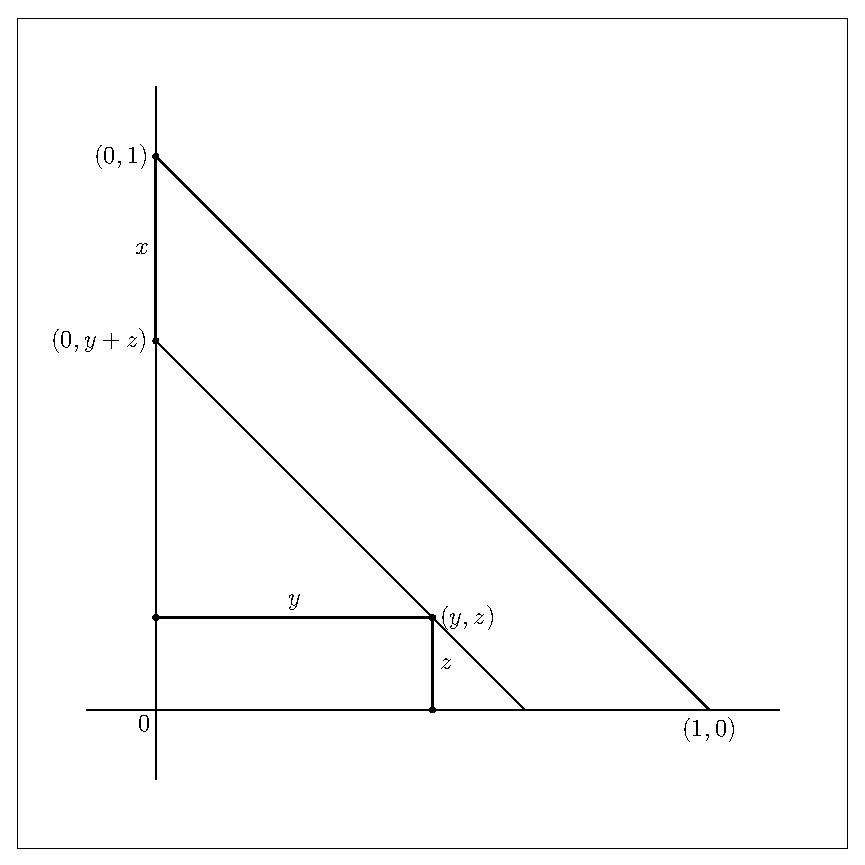
\includegraphics[width=\textwidth]{finmod.eps}
      \caption{\footnotesize The statistical model of the
        2-dimensional simplex $\mathbb{S}^{2}$. $y$ and $z$ are the
        parameters, whereas $x$ is fully determined by $y$ and $z$.
        $x,y,z$ represent the probabilities
        $P(X_{1}),P(X_{2}),P(X_{3})$ on an outcome space
        $\Omega=\{\omega_{1},\omega_{2},\omega_{3}\}$, where $X_{i}$
        is the proposition corresponding to the atomic outcome
        $\omega_{i}$. The point $(y,z)$ corresponds to the numbers in
        {\xample}~\ref{ex:holmes}.}
      \label{fig:finmod}
    \end{minipage}
\end{figure}

\begin{figure}[ht!]
    \begin{minipage}[h]{.7\linewidth}
      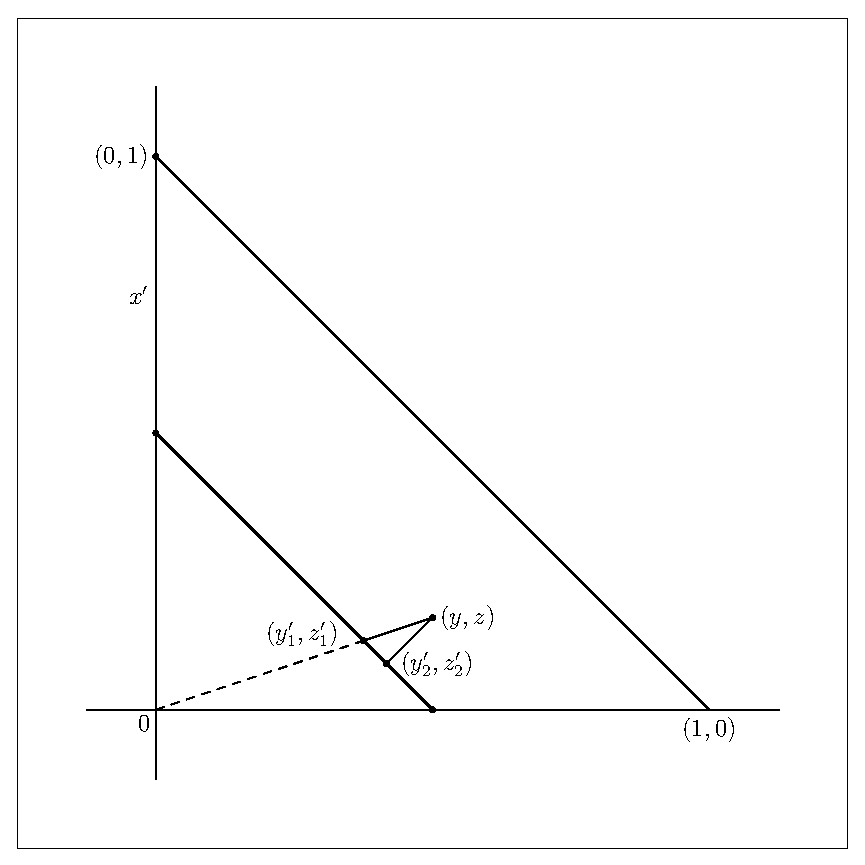
\includegraphics[width=\textwidth]{finmoe.eps}
      \caption{\footnotesize Illustration of an affine constraint.
        This is a Jeffrey-type updating scenario. While $x=1/3$ as in
        {\igure}~\ref{fig:finmod}, the updated $x'=1/2$. These are
        again the numbers of {\xample}~\ref{ex:holmes}. There appear
        to be two plausible ways to update $(y,z)$ to $(y',z')$. One
        way, which we will call Jeffrey conditioning, follows the line
        to the origin of the coordinate system. It accords with our
        intuition that as $x'\rightarrow{}1$, the updated $(y',z')$ is
        continuous with standard conditioning. The other way, which in
        chapter~\ref{chp:gahrihoo} I will call LP conditioning, uses
        the shortest geometric distance from $(y,z)$ to determine
        $(y',z')$. This case is illustrated in three dimensions (not
        using statistical parameters) in
        {\igure}~\ref{fig:threepoints}. One of the main points of this
        dissertation is that the ambivalence between updating methods
        can be resolved by using cross-entropy rather than Euclidean
        distance. Jeffrey conditioning gives us the updated
        probability distribution which minimally diverges from the
        relatively prior probability distribution in terms of
        cross-entropy.}
      \label{fig:finmoe}
    \end{minipage}
\end{figure}

As long as constraints of the form (\ref{eq:ahghaega}) are consistent,
they identify a subset of the simplex $\mathbb{S}^{n-1}$ which is an
affine subset. That is why we call them affine constraints. The affine
nature of the subset guarantees that the subset is closed and convex
(see \scite{8}{paris06}{66}). 

\begin{quotex}
  \beispiel{More Than One Half}\label{ex:ailehooc} A coin for which I
  have excellent evidence that it is fair is about to be flipped. My
  prior probability that the coin will land tails is $0.5$. A demon,
  whom I inductively know to be reliable about the future chances of
  events, tells me that on the next flip the probability for tails is
  greater than $0.5$ (see \scite{8}{landeswilliamson13}{3557}). 
\end{quotex}

If the constraint is non-affine, as in {\xample}~\ref{ex:ailehooc}, we
have no such guarantees. This causes problems largely orthogonal to
more important epistemic issues, contra Landes and Williamson, who use
this issue to stick the label of irrationality to \textsc{pme} in an
otherwise solid defence of \textsc{pme} (for more detail on affine
constraints see \scite{7}{csiszar67}{}; \scite{8}{williams80}{137};
\scite{8}{howsonfranklin94}{456}; \scite{8}{uffink96}{7};
\scite{8}{paris06}{66}; \scite{8}{debbahmueller05}{1673};
\scite{8}{williamson11}{5}; and Paul Penfield's lecture notes
\texttt{http://www-mtl.mit.edu/Courses/6.050/2013/notes},
section~9.4). 

Note that some epistemologists defend a position which requires all
affine constraints to be solved by standard conditioning (for example
Jan van Campenhout and Thomas Cover, who consider \textsc{pme} a
special case of Bayes' Theorem, see \scite{11}{campenhoutcover81}{};
\scite{7}{skyrms85}{}, which van Fraassen considers \qeins{the most
  sensitive treatment so far} in his \scite{10}{fraassen93}{313};
\scite{8}{skyrms86}{237}; \scite{8}{howsonfranklin94}{461}; and
\scite{7}{grovehalpern97}{}, making this case for the \emph{Judy
  Benjamin} problem treated in chapter~\ref{chp:eeyijeen} below).

An affine constraint makes it possible to find points in the subset
that are minimally distant from the point corresponding to the prior
probability distribution. Naively, we might use the Euclidean distance
to determine the minimally distant point (for example in
\scite{7}{joyce98}{}; or \scite{7}{leitgebpettigrew10i}{}).
Chapter~\ref{chp:gahrihoo} shows that such a procedure would put us at
odds with a host of reasonable intuitions. In the next subsection, I
am providing a sketch for a different approach: information theory.

\section{Information Theory}
\label{sec:oxiequei}

\subsection{Shannon Entropy}
\label{subsec:thahcubu}

Information theory is rooted in the consideration of communication
over noisy channels. Since most channels transmit information with
errors, before Shannon the prevailing thought was that in order to
reduce the probability of error, redundancy needed to be increased. No
pain, no gain. Shannon's noisy-channel coding theorem proves this
intuition to be false. Information can be communicated over a noisy
channel at a non-zero rate with arbitrarily small error probability.
The maximum rate for which this is possible is called the capacity of
the channel (see \scite{8}{mackay03}{14f}).

To prove this remarkable result and calculate the capacity of a
channel, Shannon needs a measure of entropy for a probability
distribution. Consider the written English language and its
distribution of Latin letters: the letter E occurs 9.1\% of the time,
whereas the letter P only occurs 1.9\% of the time. There is a certain
inefficiency in coding a message by giving as much space to symbols
that contain less information than others. The P contains more
information than an E, and in general consonants contain more
information than vowels. Codes in which there are fewer of these
inefficiencies have higher entropy. Entropy is therefore based on the
probability distribution of the code symbols. 

Let $X_{n}$ be an ensemble $(x,\mathcal{A}_{X_{n}},P_{X_{n}})$
($P_{X_{n}}$ will be abbreviated $P_{n}$ in the following), where $x$
is the outcome of a random variable, $P_{n}$ is the probability
distribution, and the outcome set $\mathcal{A}_{X_{n}}$ is an alphabet
with $n$ letters. We want a measure of entropy that has the following
properties (see \scite{7}{khinchin57}{}, for these axioms; I gleaned
them from \scite{8}{guiasu77}{9}):

\begin{enumerate}[(K1)]
\item For any $n$, the function
  $H_{n}(P_{n}(x_{1}),\ldots,P_{n}(x_{n}))$ is a continuous and
  symmetric function with respect to all of its arguments.
\item For every $n$, we have
  $H_{n+1}(P_{n}(x_{1}),\ldots,P_{n}(x_{n}),0)=H_{n}(P_{n}(x_{1}),\ldots,P_{n}(x_{n}))$.
\item For every $n$, we have the inequality
  $H_{n}(P_{n}(x_{1}),\ldots,P_{n}(x_{n}))\leq{}H_{n}(1/n,\dots,1/n)$.
\item If the conditions in (\ref{eq:oupiahel}) hold for $\pi_{kl}$, the consequent in
  (\ref{eq:oothaedo}) is true.
\end{enumerate}

{\noindent}For K4, the conditions are

\begin{equation}
  \label{eq:oupiahel}
  \pi_{kl}\geq{}0,\sum_{k=1}^{n}\sum_{l=1}^{m_{k}}\pi_{kl}=1,P_{n}(x_{k})=\sum_{l=1}^{m_{k}}\pi_{kl},M=\sum_{k=1}^{n}m_{k}
\end{equation}

{\noindent}and the consequent is

\begin{equation}
  \label{eq:oothaedo}
  \begin{array}{l}
    \displaystyle H_{nM}(\pi_{11},\ldots,\pi_{nm_{n}})= \\
    \displaystyle H_{n}(P_{n}(x_{1}),\ldots,P_{n}(x_{n}))+\sum_{k=1}^{n}P_{n}(x_{k})H_{m_{k}}\left(\frac{\pi_{k1}}{P_{n}(x_{k})},\ldots,\frac{\pi_{km_{k}}}{P_{n}(x_{k})}\right). \\
  \end{array}
\end{equation}

K1--3 are self-explanatory. K4 requires that the entropy of a product
code is obtained by adding the entropy of one component to the entropy
of the other component conditioned by the first one. Given Khinchin's
axioms, theorem 1.1 in Silviu Guia{\c{s}}u's book proves that 

\begin{equation}
  \label{eq:kualiaku}
  H_{n}(P_{n}(x_{1}),\ldots,P_{n}(x_{n}))=-c\sum_{k=1}^{n}P_{n}(x_{k})\log{}P_{n}(x_{n})
\end{equation}

{\noindent}Leaving off the subscript $n$ (which is predetermined by the
cardinality of the alphabet) and taking $c=1$, 

\begin{equation}
  \label{eq:oowoongu}
  H(P(x_{1}),\ldots,P(x_{n}))=-\sum_{k=1}^{n}P(x_{k})\log{}P(x_{n})
\end{equation}

{\noindent}is called the Shannon entropy (see \scite{7}{shannon48}{}).

\subsection{Kullback-Leibler Divergence}
\label{subsec:sihaivei}

I could use the Shannon entropy as a first pass to isolate a
probability distribution from a candidate set determined by an affine
constraint.

\begin{quotex}
  \textsc{original pme} A rational agent accepts the probability
  distribution as her partial beliefs which is maximal in terms of
  Shannon entropy while according with evidential constraints.
\end{quotex}

{\noindent}The problem with \textsc{original pme} is that it does not
take into account a relatively prior probability distribution and is
therefore inconsistent with the former of the two basic commitments of
Bayesians: the partial beliefs of a rational agent (i) depend on a
prior probability and (ii) are obtained by standard conditioning if
applicable. Like the likelihood principle, \textsc{original pme} does
not make reference to a prior probability and is therefore unsuitable
from a Bayesian point of view.

In order to fix this, we need the concept of cross-entropy. Whereas
maximizing the Shannon entropy gives us the most efficient code given
a set of constraints (if they are affine constraints, this code will
be uniquely distributed), minimizing cross-entropy gives us the code
with respect to which the relatively prior probability distribution is
most efficient. Cross-entropy measures how much information is lost
when a message is coded using a code optimized for the relatively
prior probability distribution rather than the \qnull{true} posterior
distribution. When I pick a posterior probability distribution
according to the principle of minimum cross-entropy or \emph{Infomin},
I pick the probability distribution that accords with my constraints
and makes the relatively prior distribution look as efficient as
possible. This is analogous to Bayesian conditionalization, where I
choose a posterior probability distribution which strikes a balance
between respecting the prior and respecting the new evidence.

To implement \emph{Infomin}, I need a measure for cross-entropy.
Again, as in K1--4, I first formulate a set of desiderata for this
function that maps two probability distributions $P_{n}$ and $Q_{n}$
to the set of real numbers. A caveat here: the cross-entropy is
conceptualized as a divergence of $P_{n}$ from $Q_{n}$ so that in the
logic of updating $Q_{n}$ is the relatively prior probability
distribution and $P_{n}$ is the posterior. I shall use the generic
label $D(P_{n},Q_{n})$ for this measure in the desiderata. I shall
also sometimes write
$D(P_{n}(x_{1}),\ldots,P_{n}(x_{n});Q_{n}(x_{1}),\ldots,Q_{n}(x_{n}))$
for $D(P_{n},Q_{n})$. This time, I gleaned the desiderata from
\scite{8}{paris06}{121}; the original proof is in
\scite{7}{kullbackleibler51}{}.

\begin{enumerate}[(KL1)]
\item For each $n$, $D(P_{n},Q_{n})$ is continuous, provided that
  $Q(x_{i})\neq{}0$ if $P(x_{i})\neq{}0$.
\item For $0<n\leq{}n_{0}$,
  $D(1/n,\ldots,1/n,0,\ldots,0;1/n_{0},\ldots,1/n_{0}))$ is strictly
  decreasing in $n$ and increasing in $n_{0}$ and is $0$ if $n=n_{0}$.
\item Provided that $Q(x_{i})\neq{}0$ if $P(x_{i})\neq{}0$, and given
  a permutation $\sigma$ of $(1,\ldots,n)$, the consequent
  (\ref{eq:eengaiya}) holds.
\item If the conditions in (\ref{eq:oupiahel}) hold for $\pi_{kl}$ and
  analogous conditions hold for $\varrho_{kl}$ (replace $P$ by $Q$),
  then the consequent in (\ref{eq:adeedaht}) is true, provided that
  $\varrho_{kl}\neq{}0$ if $\pi_{kl}\neq{}0$.
\end{enumerate}

{\noindent}For KL3, the consequent is

\begin{equation}
  \label{eq:eengaiya}
  \begin{array}{l}
    \displaystyle
    D(P_{n}(x_{1}),\ldots,P_{n}(x_{n});Q_{n}(x_{1}),\ldots,Q_{n}(x_{n}))= \\
    D(P_{n}(x_{\sigma(1)}),\ldots,P_{n}(x_{\sigma(n)});Q_{n}(x_{\sigma(1)}),\ldots,Q_{n}(x_{\sigma(n)})) \\
  \end{array}
\end{equation}

{\noindent}For KL4, the consequent is

\begin{equation}
  \label{eq:adeedaht}
  \begin{array}{l}
    \displaystyle D(\pi_{11},\ldots,\pi_{nm_{n}};\varrho_{11},\ldots,\varrho_{nm_{n}})= \\
    \displaystyle D(P_{n}(x_{1}),\ldots,P_{n}(x_{n});Q_{n}(x_{1}),\ldots,Q_{n}(x_{n}))+ \\
    \displaystyle \sum_{k=1}^{n}P_{n}(x_{k})D\left(\frac{\pi_{k1}}{P_{n}(x_{k})},\ldots,\frac{\pi_{km_{k}}}{P_{n}(x_{k})};\frac{\varrho_{k1}}{P_{n}(x_{k})},\ldots,\frac{\varrho_{km_{k}}}{P_{n}(x_{k})}\right). \\
  \end{array}
\end{equation}

{\noindent}These desiderata give us the solution

\begin{equation}
  \label{eq:enuamich}
  D(P_{n},Q_{n})=c\sum_{i=1}^{n}P_{n}(x_{i})\log\frac{P_{n}(x_{i})}{Q_{n}(x_{i})}
\end{equation}

{\noindent}which is fulfilled by the Kullback-Leibler divergence $D_{\mbox{\tiny
    KL}}$, again setting $c=1$,

\begin{equation}
  \label{eq:xaingouw}
  D_{\mbox{\tiny KL}}(P_{n},Q_{n})=\sum_{i=1}^{n}P_{n}(x_{i})\log\frac{P_{n}(x_{i})}{Q_{n}(x_{i})}.
\end{equation}

Now let us work on a more useful definition of \textsc{pme}. To
standard Bayesian commitments, \textsc{pme} adds

\begin{quotex}
  Update relatively prior distributions under formalized constraints
  in accordance with information theory and a commitment to keep the
  entropy maximal, if constraints are synchronic, and the
  cross-entropy minimal, if they are diachronic.
\end{quotex}

{\noindent}This corresponds to the intuition that we ought not to gain
information where the additional information is not warranted by the
evidence. Some want to drive a wedge between the synchronic rule to
keep the entropy maximal (\textsc{pme}) and the diachronic rule to
keep the cross-entropy minimal (\emph{Infomin}) (for this objection
see \scite{8}{walley91}{270f}). Here is a brief excursion to dispel
this worry.

\begin{quotex}
  \beispiel{Piecemeal Learning}\label{ex:piecemeal} Consider a bag
  with blue, red, and green tokens. You know that ($C'$) at least 50\%
  of the tokens are blue. Then you learn that ($C''$) at most 20\% of
  the tokens are red.
\end{quotex}

The synchronic norm, on the one hand, ignores the diachronic dimension
and prescribes the probability distribution which has the maximum
entropy and obeys both ($C'$) and ($C''$). The three-dimensional
vector containing the probabilities for blue, red, and green is
$(\frac{1}{2},\frac{1}{5},\frac{3}{10})$. The diachronic norm, on the
other hand, processes ($C'$) and ($C''$) sequentially, taking in its
second step $(\frac{1}{2},\frac{1}{4},\frac{1}{4})$ as its prior
probability distribution and then diachronically updating to
$(\frac{8}{15},\frac{1}{5},\frac{4}{15})$.

The information provided in a problem calling for the synchronic norm
and the information provided in a problem calling for the diachronic
norm is different, as temporal relations and their implications for
dependence between variables clearly matter. In
{\xample}~\ref{ex:piecemeal}, we might have relevantly received
information ($C''$) before ($C'$) (\qnull{before} may be understood
logically rather than temporally) so that \emph{Infomin} updates in
its last step $(\frac{2}{5},\frac{1}{5},\frac{2}{5})$ to
$(\frac{1}{2},\frac{1}{6},\frac{1}{3})$. Even if ($C'$) and ($C''$)
are received in a definite order, the problem may be phrased in a way
that indicates independence between the two constraints. In this case,
the synchronic norm is the appropriate norm to use. \emph{Infomin}
does not assume such independence and therefore processes the two
pieces of information separately. Disagreement arises when
observations are interpreted differently, not because \textsc{pme} and
\emph{Infomin} are inconsistent with each other. 

The fault line for commutativity is actually located between standard
conditioning (which is always commutative) and Jeffrey conditioning
(which is sometimes non-commutative). Huttegger explains:

\begin{quotex}
  This has caused some concerns as to whether probability kinematics
  is a rational way to update beliefs (\scite{7}{doering99}{};
  \scite{7}{lange00}{}; and \scite{7}{kelly08}{}). I agree with Wagner
  and Joyce that these concerns are misguided (see
  \scite{7}{wagner02}{}; and \scite{7}{joyce10ii}{}). As Joyce points
  out, probability kinematics is non-commutative exactly when it
  should be; namely, when belief revision destroys information
  obtained in previous updates. \scite{3}{huttegger15}{628}
\end{quotex}

{\noindent}In the following, I will assume that \textsc{pme} and
\emph{Infomin} are compatible and part of the toolkit at the disposal
of \textsc{pme}.

The first question to ask is if \textsc{pme} is compatible with the
Bayesian commitment to standard conditioning. The answer is yes.
Better yet, \textsc{pme} also agrees with Jeffrey's extension to
standard conditioning, now commonly called Jeffrey conditioning.

A proof that \textsc{pme} generalizes standard conditioning is in
\scite{7}{williams80}{}. A proof that \textsc{pme} generalizes Jeffrey
conditioning is in \scite{7}{jeffrey65}{}. I will give my own simple
proofs here that are more in keeping with the notation in the body of
the dissertation. An interested reader can also apply these proofs to
show that \textsc{pme} generalizes Wagner conditioning, but not
without simplifications that compromise mathematical rigour. The more
rigorous proof for the generalization of Wagner conditioning is in
section~\ref{sec:uodeigei}.

I assume finite (and therefore discrete) probability distributions.
For countable and continuous probability distributions, the reasoning
is largely analogous (for an introduction to continuous entropy see
\scite{8}{guiasu77}{16ff}; for an example of how to do a proof of this
section for continuous probability densities see
\scite{7}{catichagiffin06}{}, and \scite{7}{jaynes78}{}; for a proof
that the stationary points of the Lagrange function are indeed the
desired extrema see \scite{8}{zubarevetal74}{55}, and
\scite{8}{coverthomas06}{410}; for the pioneer of the method applied
in this section see \scite{8}{jaynes78}{241ff}). Before I address
standard conditioning in subsection~\ref{subsec:yeequika} and 
Jeffrey conditioning in subsection~\ref{subsec:ukotooje}, I will
present Jaynes method in the next subsection.

\subsection{Jaynes' Constraint Rule}
\label{subsec:choiwohk}

This subsection provides a concise but comprehensive summary of
Jaynes' constraint rule not easily obtainable in the literature.
Jaynes applied it to the \emph{Brandeis Dice} Problem (see
\scite{8}{jaynes89}{243}, and {\xample}~\ref{ex:brandeis}), but does
not give a mathematical justification.

Let $f$ be a probability distribution on a finite space
$x_{1},\ldots,x_{m}$ that fulfills the constraint 
\begin{equation}
  \label{eq:constraint}
\sum_{i=1}^{m}r(x_{i})f(x_{i})=\alpha.
\end{equation}

{\noindent}An affine constraint can always be expressed by assigning a value to
the expectation of a probability distribution (see
\scite{7}{hobson71}{}), as in (\ref{eq:ahghaega}). In Judy Benjamin's
case (see chapter~\ref{chp:eeyijeen}), for example, let
$r(x_{1})=0, r(x_{2})=1-{\qvu}, r(x_{3})=-{\qvu}\mbox{ and }\alpha=0$.
Because $f$ is a probability distribution it fulfills
\begin{equation}
  \label{eq:unity}
\sum_{i=1}^{m}f(x_{i})=1
\end{equation}

{\noindent}We want to maximize Shannon's entropy, given the constraints
({\ref{eq:constraint}}) and ({\ref{eq:unity}}),
\begin{equation}
  \label{eq:entropy}
-\sum_{i=1}^{m}f(x_{i})\ln(x_{i})
\end{equation}

{\noindent}We use Lagrange multipliers to define the functional
\begin{equation}
  \label{eq:functional}
J(f)=-\sum_{i=1}^{m}f(x_{i})\ln{}f(x_{i})+\lambda_{0}\sum_{i=1}^{m}f(x_{i})+\lambda_{1}\sum_{i=1}^{m}r(x_{i})f(x_{i})
\end{equation}
{\noindent}and differentiate it with respect to $f(x_{i})$
\begin{equation}
  \label{eq:funder}
\frac{\partial{}J}{\partial{}f(x_{i})}=-\ln(f(x_{i}))-1+\lambda_{0}+\lambda_{1}r(x_{i})
\end{equation}

{\noindent}Set ({\ref{eq:funder}}) to $0$ to find the necessary condition to
maximize ({\ref{eq:entropy}})
\begin{equation}
  \label{eq:coverthomas}
g(x_{i})=e^{\lambda_{0}-1+\lambda_{1}r(x_{i})}
\end{equation}

{\noindent}This is the Gibbs distribution. We still need to do two things: (a)
show that the entropy of $g$ is maximal, and (b) show how to find
$\lambda_{0}$ and $\lambda_{1}$. (a) is shown in Theorem 12.1.1 in
Cover and Thomas \scite{1}{coverthomas06}{} and there is no reason to
copy it here. 

For (b), let
\begin{equation}
  \label{eq:l1}
\lambda_{1}=-\beta
\end{equation}
\begin{equation}
  \label{eq:zet}
Z(\beta)=\sum_{i=1}^{m}e^{-\beta{}r(x_{i})}
\end{equation}
\begin{equation}
  \label{eq:l0}
\lambda_{0}=1-\ln(Z(\beta))
\end{equation}

{\noindent}To find $\lambda_{0}$ and $\lambda_{1}$ we introduce the constraint
\begin{equation}
  \label{eq:logcon}
-\frac{\partial}{\partial{}\beta}\ln(Z(\beta))=\alpha
\end{equation}

To see how this constraint gives us $\lambda_{0}$ and $\lambda_{1}$,
Jaynes' solution of the \emph{Brandeis Dice} Problem is a helpful
example. We are, however, interested in a general proof that this
choice of $\lambda_{0}$ and $\lambda_{1}$ gives us the probability
distribution maximizing the entropy. That $g$ so defined maximizes the
entropy is shown in (a). We need to make sure, however, that with this
choice of $\lambda_{0}$ and $\lambda_{1}$ the constraints
({\ref{eq:constraint}}) and ({\ref{eq:unity}}) are also fulfilled.

First, we show

\begin{equation}
  \label{eq:unishow}
  \begin{array}{l}
\displaystyle \sum_{i=1}^{m}g(x_{i})=\sum_{i=1}^{m}e^{\lambda_{0}-1+\lambda_{1}r(x_{i})}=e^{\lambda_{0}-1}\sum_{i=1}^{m}e^{\lambda_{1}r(x_{i})}= \\
\displaystyle e^{-\ln(Z(\beta))}Z(\beta)=1 \\
  \end{array}
\end{equation}

{\noindent}Then, we show, by differentiating $\ln(Z(\beta))$ using the
substitution $x=e^{-\beta}$

\begin{equation}
  \label{eq:feicoxai}
  \begin{array}{l}
\displaystyle \alpha=-\frac{\partial}{\partial{}\beta}\ln(Z(\beta))=-\frac{1}{\sum_{i=1}^{m}x^{r(x_{i})}}\left(\sum_{i=1}^{m}r(x_{i})x^{r(x_{i})-1}\right)(-x)= \\
\displaystyle \frac{\sum_{i=1}^{m}r(x_{i})x^{r(x_{i})}}{\sum_{i=1}^{m}x^{r(x_{i})}} \\
  \end{array}
\end{equation}

{\noindent}And, finally,

\begin{equation}
  \label{eq:ayohgeix}
  \begin{array}{l}
\displaystyle \sum_{i=1}^{m}r(x_{i})g(x_{i})=\sum_{i=1}^{m}r(x_{i})e^{\lambda_{0}-1+\lambda_{1}r(x_{1})}=e^{\lambda_{0}-1}\sum_{i=1}^{m}r(x_{i})e^{\lambda_{1}r(x_{1})}= \\
\displaystyle e^{\lambda_{0}-1}\sum_{i=1}^{m}r(x_{i})x^{r(x_{i})}=\alpha{}e^{\lambda_{0}-1}\sum_{i=1}^{m}x^{r(x_{i})}=\alpha{}e^{\lambda_{0}-1}\sum_{i=1}^{m}e^{-\beta{}r(x_{i})}= \\
\displaystyle \alpha{}Z(\beta)e^{\lambda_{0}-1}=\alpha{}Z(\beta))e^{-\ln(Z(\beta))}=\alpha. \\
  \end{array}
\end{equation}

{\noindent}Anticipating chapter~\ref{chp:eeyijeen}, filling in the
variables from Judy Benjamin's scenario gives us result
({\ref{eq:vmax}}). The lambdas are:

\begin{equation}
  \label{eq:diquefuc}
\lambda_{0}=1-\ln\left(\sum_{i=1}^{m}e^{\lambda_{1}r(x_{i})}\right)\hspace{.3in}
\lambda_{1}=\ln{}{\qvu}-\ln(1-{\qvu})\notag
\end{equation}

A proof with similar intentions as this subsection can be found in
Paul Penfield's lecture notes
\texttt{http://www-mtl.mit.edu/Courses/6.050/2013/notes},
subsection~9.6.3.

\subsection{Standard Conditioning}
\label{subsec:yeequika}

Let $y_{i}$ (all $y_{i}\neq{}0$) be a finite relatively prior
probability distribution summing to $1$, $i\in{}I$. Let $\hat{y}_{i}$
be the posterior probability distribution derived from standard
conditioning with $\hat{y}_{i}=0$ for all $i\in{}I'$ and
$\hat{y}_{i}\neq{}0$ for all $i\in{}I''$, $I'\cup{}I''=I$. $I'$ and
$I''$ specify the standard event observation. Standard conditioning
requires that

\begin{equation}
  \label{eq:sc}
  \hat{y}_{i}=\frac{y_{i}}{\sum_{k\in{}I''}y_{k}}.
\end{equation}

{\noindent}To solve this problem using \textsc{pme}, we want to minimize the
cross-entropy with the constraint that the non-zero $\hat{y}_{i}$ sum to
$1$. The Lagrange function is (writing in vector form
$\hat{y}=(\hat{y}_{i})_{i\in{}I''}$)

\begin{equation}
  \label{eq:sclag}
  \Lambda(\hat{y},\lambda)=\sum_{i\in{}I''}\hat{y}_{i}\ln\frac{\hat{y}_{i}}{y_{i}}+\lambda\left(1-\sum_{i\in{}I''}\hat{y}_{i}\right).
\end{equation}

{\noindent}Differentiating the Lagrange function with respect to $\hat{y}_{i}$ and
setting the result to zero gives us

\begin{equation}
  \label{eq:sc1}
  \hat{y}_{i}=y_{i}e^{\lambda-1}
\end{equation}

{\noindent}with $\lambda$ normalized to

\begin{equation}
  \label{eq:sc2}
  \lambda=-1+\ln{}\sum_{i\in{}I''}y_{i}.
\end{equation}

{\noindent}(\ref{eq:sc}) follows immediately. \textsc{pme} generalizes standard conditioning.

\subsection{Jeffrey Conditioning}
\label{subsec:ukotooje}

For this subsection, I am using a special notation that I develop in
section~\ref{sec:uodeigei}. Even though thematically this subsection
belongs here, it depends on understanding the notation introduced in
chapter~\ref{chp:eejiegei}. The reader may want to skip this
subsection and return to it later. The conclusion stands that
\textsc{pme} generalizes Jeffrey conditioning. 

Let $\theta_{i},i=1,\ldots,n$ and $\omega_{j},j=1,\ldots,m$ be finite
partitions of the event space with the joint prior probability matrix
$(y_{ij})$ (all $y_{ij}\neq{}0$). Let $\kappa$ be defined as in
section~\ref{sec:uodeigei}, with (\ref{eq:m1}) true (remember that in
section~\ref{sec:uodeigei}, (\ref{eq:m1}) is no longer required). Let
$P$ be the relatively prior probability distribution and $\hat{P}$ the
posterior probability distribution.

Let $\hat{y}_{ij}$ be the posterior probability distribution derived
from Jeffrey conditioning with

\begin{equation}
  \label{eq:jc1}
  \sum_{i=1}^{n}\hat{y}_{ij}=\hat{P}(\omega_{j})\mbox{ for all }j=1,\ldots,m
\end{equation}

{\noindent}Jeffrey conditioning requires that for all $i=1,\ldots,n$

\begin{equation}
  \label{eq:jc2}
  \hat{P}(\theta_{i})=\sum_{j=1}^{m}P(\theta_{i}|\omega_{j})\hat{P}(\omega_{j})=\sum_{j=1}^{m}\frac{y_{ij}}{P(\omega_{j})}\hat{P}(\omega_{j})
\end{equation}

{\noindent}Using \textsc{pme} to get the posterior distribution
$(\hat{y}_{ij})$, the Lagrange function is (writing in vector form
$\hat{y}=(x_{11},\ldots,x_{n1},\ldots,x_{nm})^{\top}$ and
$\lambda=(\lambda_{1},\ldots,\lambda_{m})^{\top}$)

\begin{equation}
  \label{eq:jclag}
  \Lambda(\hat{y},\lambda)=\sum_{i=1}^{n}\sum_{j=1}^{m}\hat{y}_{ij}\ln\frac{\hat{y}_{ij}}{y_{ij}}+\sum_{j=1}^{m}\lambda_{j}\left(\hat{P}(\omega_{j})-\sum_{i=1}^{n}\hat{y}_{ij}\right).
\end{equation}

{\noindent}Consequently,

\begin{equation}
  \label{eq:jc4}
  \hat{y}_{ij}=y_{ij}e^{\lambda_{j}-1}
\end{equation}

{\noindent}with the Lagrangian parameters $\lambda_{j}$ normalized by

\begin{equation}
  \label{eq:jc5}
  \sum_{i=1}^{n}y_{ij}e^{\lambda_{j}-1}=\hat{P}(\omega_{j})
\end{equation}

{\noindent}(\ref{eq:jc2}) follows immediately. \textsc{pme}
generalizes Jeffrey conditioning.

\section{Pragmatic, Axiomatic, and Epistemic Justification}
\label{sec:vichaina}

\subsection{Three Approaches}
\label{subsec:eiphethe}

There are various ways in which an explanatory theory of a rational
agent's partial beliefs can be justified. The rational agent is a
relevant idealization, relevant in the sense that there may be a
different explanatory theory of an effective human reasoner's partial
beliefs. The rational agent models an inductive logic, not dissimilar
to the inference relationships that model deductive logic and may also
be relevant idealizations of effective human deductive reasoning.

In this dissertation, I am assuming that a rational agent already has
quantitative partial beliefs (also called credences) about certain
propositions and that she reasons as a Bayesian, i.e.\ her credences
are probabilistic (obey Kolmogorov's axioms) and she updates them
using standard conditioning whenever standard conditioning is
applicable. This assumption is controversial. There are a few places
in this dissertation where I provide some justification for them, but
the focus is the next step once the Bayesian elements are already in
place. 

I defend the thesis that (i) rational agents have sharp credences and
(ii) update them in accordance with norms based on and in agreement
with information theory. Neither the sharp credences nor the
information update is a necessary feature of recent Bayesian
epistemology. On the contrary, when I defend my claims, I anecdotally
find that most Bayesians prefer indeterminate credal states and an
eclectic approach to updating. This section is less concerned with a
defence of my claims than with the question of what a defence would
need to do in order to be successful. Partial belief epistemologists
have varying preferences about what justifies their theories. 

For ease of exposition, I am condensing them to three major
approaches: the psychological, the formal, and the philosophical. My
hope is that a defence of (i) and (ii) succeeds on all three levels.
Since all three approaches have explanatory virtue, one would also
hope that they converge and settle on compatible solutions to the
question of which partial beliefs rational agents entertain.
(J{\"u}rgen Landes and Jon Williamson similarly show how three norms
converge in justifying \textsc{pme}: a probability norm, a calibration
norm, and an equivocation norm, see \scite{7}{landeswilliamson13}{}.)
Information theory and its virtues across all three levels support
this convergence.

Here is a more detailed description of what I mean by the
psychological, the formal, and the philosophical approach, which I
cash out as providing pragmatic, axiomatic, and epistemic
justification for the partial beliefs of a rational agent.

\subsection{The Psychological Approach}
\label{subsec:oopiasee}

The psychological approach justifies partial beliefs by highlighting
their pragmatic virtues. Frank Ramsey and Bruno de Finetti were the
first to substantiate this approach (see \scite{7}{ramsey26}{}; and de
Finetti \scite{11}{definetti31}{}). A system of partial beliefs
corresponds to a willingness to make decisions in the light of these
beliefs, most helpfully to purchase a bet on a proposition $p$ costing
\$$x$ with a return of \$$1$ if the proposition turns out to be true
and no return if the proposition turns out to be false.

Both synchronic and diachronic Dutch-book arguments demonstrate the
constraints that rational agents have with respect to their partial
beliefs lest they fall prey to arbitrage opportunities. The most vocal
critics of the synchronic argument are Colin Howson and Peter Urbach
(loc.\ cit., but see also \scite{8}{earman92}{38f}). The diachronic
arguments, however, are significantly more controversial and less
supported in the literature than the synchronic arguments originally
formulated by de Finetti (for the diachronic argument supporting
standard conditioning see \scite{7}{armendt80}{}; and
\scite{7}{lewis99}{}; for criticism see
\scite{8}{howsonfranklin94}{458}). Jon Williamson, interestingly,
thinks that the diachronic argument fails because it supports Bayesian
conditionalization \emph{against} \textsc{pme}, with which it is
incompatible and to which it must cede (see
\scite{7}{williamson11}{}). The idea that Bayesian conditionalization
and \textsc{pme} conflict can be found in other places as well (see
\scite{8}{seidenfeld79}{432f}; \scite{7}{shimony85}{};
\scite{8}{fraassen93}{288ff}; \scite{8}{uffink95}{14};
\scite{8}{howsonurbach06}{278}; and
\scite{8}{neapolitanjiang14}{4012}), but the usual interpretation is
that the conflict undermines \textsc{pme}.

\subsection{The Formal Approach}
\label{subsec:ahghuato}

The formal approach justifies partial beliefs by providing an
axiomatic system which coheres with intuitions we have about partial
beliefs and limits the partial belief functions fulfilling the formal
constraints. The pioneer of this method is Richard Cox in his landmark
article \qeins{Probability, Frequency and Reasonable Expectation.} The
idea is simple and can be surprisingly powerful: formalize reasonable
expectations and apply them to yield unique solutions, so that for
example only partial beliefs fulfilling Bayesian requirements also
fulfill the reasonable expectations. The idea is controversial,
especially when it leads to unique solutions.

It is often possible to weaken the assumptions such that families of
solutions, rather than unique solutions, fulfill the axioms. This is
the case for Carnap's con\-ti\-nuum of inductive methods (see
\scite{7}{carnap52}{}) and the R{\'e}nyi entropy, which generalizes
Shannon's entropy and yields families of credence functions fulfilling
maximum entropy requirements (see \scite{7}{uffink95}{}, who
criticizes and weakens the assumptions of \scite{7}{shorejohnson80}{},
a paradigmatic example for the formal approach supporting
\textsc{pme}; and \scite{7}{huisman14}{}, who uses this idea to solve
the \emph{Judy Benjamin} problem in chapter~\ref{chp:eeyijeen} with
indeterminate credal states).

There is a sense in which both the psychological and the philosophical
approach are formal approaches as well, starting with a set of axioms
and identifying the credence functions that fulfill them. I am setting
the formal approach aside when it appears that the uniqueness result
is kept in mind as a trajectory in formulating the axioms. Often,
there is resistance to such a manipulation of the initial conditions
in order to achieve the final result of uniqueness (see the above
weakening of the axioms). The formal approach, however, considers
uniqueness itself a desired outcome with justificatory force. There is
something at least interesting about the set of axioms that gives us a
unique solution, even though each axiom still needs to pass the
rigorous test of plausibility compared to its alternatives. 

For Ramsey and de Finetti, the salient axiom is invulnerability to
arbitrage opportunities and does decidedly not yield uniqueness.
Subjective probabilities can range wildly between rational agents, as
long as they adhere to the laws of probability. Bas van Fraassen
argues that calibration requirements mandate the use of standard
conditioning once a relatively prior probability distribution is in
place (see van Fraassen, \scite{11}{fraassen89}{}). The calibration
requirement is both psychological and formal in the sense that it is
based on pragmatic considerations about an agent's psychology and
behaviour, especially her need to have beliefs and states of the world
calibrated, but also on a formal apparatus that gives us a unique
result for conditioning on new information. Joyce provides the
philosophical counterpart (see \scite{7}{joyce98}{}), where the
salient axiom is gradational accuracy (which is philosophical rather
than psychological in its nature) and again standard conditioning
follows as the uniquely mandated updating method fulfilling the axiom.

In a Jeffrey-type updating scenario, where standard conditioning
cannot be applied, there are similar attempts to isolate a unique
updating method. This method is usually Jeffrey conditioning, for
which there are dynamic coherence arguments (see
\scite{7}{armendt80}{}; \scite{7}{goldstein83}{}; and
\scite{7}{skyrms86}{}), met with critical resistance in the literature
(see \scite{7}{levi87}{}; \scite{7}{christensen99}{};
\scite{7}{talbott91}{}; \scite{7}{maher92}{}; and
\scite{7}{howsonurbach06}{}). Remarkably, Joyce's norm of gradational
accuracy mandates a different unique updating method in Jeffrey-type
updating scenarios, LP conditioning (see
\scite{7}{leitgebpettigrew10ii}{}). I will look at this anomaly in
great detail in chapter~\ref{chp:gahrihoo}.

Sometimes neither standard conditioning nor Jeffrey conditioning can
be applied, even though the constraint is affine. In this case, we can
develop a justification of \textsc{pme} using the axiomatic approach
(see \scite{7}{shorejohnson80}{}; \scite{7}{tikochinskyetal84}{}; and
\scite{7}{skilling88}{}). Criticism of \textsc{pme} focuses either on
the strength of the assumptions (and weakening them, as in
\scite{7}{uffink96}{}) or on deductive implications of the axioms that
are inconsistent with epistemic intuitions we have about particular
cases (the paradigm case is the \emph{Judy Benjamin} problem, see van
Fraassen, \scite{11}{fraassen81}{}). 

The following quotes illustrate the skepticism entertained by many
about \textsc{pme} as a general updating procedure for affine
constraints:

\begin{quotex}
  There has been considerable interest recently in maximum entropy
  methods, especially in the philosophical literature. Example 5.1
  suggests that any claims to the effect that maximum-entropy revision
  is the only correct route to probability revision should be viewed
  with considerable caution because of its strong dependence on the
  measure of closeness being used. \scite{3}{diaconiszabell82}{829}
\end{quotex}

\begin{quotex}
  It will come as no surprise to those who have studied the relation
  of \textsc{maxent} to conditionalization in a larger space that
  there are many strategies which conflict with \textsc{maxent} and
  yet satisfy these conditions for coherence. \scite{3}{skyrms86}{241}
\end{quotex}

\begin{quotex}
  None of the arguments for the PME, when regarded as a general method
  for generating precise probabilities, is at all compelling.
  \scite{3}{walley91}{271}
\end{quotex}

\begin{quotex}
  The fact that Jeffrey's rule coincides with \textsc{maxent} is
  simply a misleading fluke, put in its proper perspective by the
  natural generalization of Jeffrey conditionalization described in
  this paper. \scite{3}{wagner92}{255}
\end{quotex}

\begin{quotex}
  We saw that simple conditionalization is actually the rule enjoined
  by the principle of minimum information in such circumstances.
  Furthermore, not to use the rule of Bayesian conditionalization, but
  some other rule, like the principle of minimum information with a
  uniform prior and constraints in the form of expectation values,
  actually entails inconsistency, i.e.\ incoherence.
  \scite{3}{howsonfranklin94}{465}
\end{quotex}

\begin{quotex}
  Maximum entropy is also sometimes proposed as a method for solving
  inference problems \ldots I think it is a bad idea to use maximum
  entropy in this way; it can give very silly answers.
  \scite{3}{mackay03}{308}
\end{quotex}

\begin{quotex}
  Maximum entropy and relative entropy have proved quite successful in
  a number of applications, from physics to natural-language modeling.
  Unfortunately, they also exhibit some counterintuitive behavior on
  certain applications. Although they are valuable tools, they should
  be used with care. \scite{3}{halpern03}{110}
\end{quotex}

\begin{quotex}
  [\textsc{pme}] essentially never gives the right results {\ldots} it
  is likely to give highly misleading answers.
  \scite{3}{gruenwaldhalpern03}{243}
\end{quotex}

\begin{quotex}
  Given the other problematic features of conditionalization we
  pointed to in Chapter 3, we feel that in linking its fortunes to the
  principle of minimum information no real advance has been made in
  justifying its adoption as an independent Bayesian principle.
  \scite{3}{howsonurbach06}{287f}
\end{quotex}

\begin{quotex}
  It is notoriously difficult to defend general procedures for
  directly updating credences on constraints. \scite{3}{moss13}{7}
\end{quotex}

My dissertation disagrees with these assessments. The strength of the
axioms, which require a unique updated probability distribution that
is minimally informative with respect to the prior probability
distribution, is defensible and does not lead to incoherence.

\subsection{The Philosophical Approach}
\label{subsec:upuxaith}

The philosophical approach justifies partial beliefs by highlighting
epistemic virtues of partial beliefs, contrasted usually with
pragmatic virtues. The idea is that there is independent appeal in
having doxastic states that are as close as possible to the truth, no
matter what their pragmatic consequences are. The manifesto of this
approach is James Joyce's article \qeins{A Nonpragmatic Vindication of
  Probabilism.} In full belief epistemology, epistemic virtue consists
in the balance between believing as many truths and disbelieving as
many falsehoods as possible. A trade-off may be involved between
valuing a low error ratio and valuing a high number of beliefs (on
which one can act, for example, and be better safe than sorry, even
when the belief is false, see \scite{7}{stephens01}{}). 

The point of this approach, however, is that pragmatic considerations
take the back seat and give priority to a rational agent's desire to
get as close as possible to reflecting the state of the world in her
epistemic state. Joyce's \emph{Norm of Gradational Accuracy}, which
generalizes the full belief norm of accuracy to partial beliefs,
succeeds in affording us a system of requirements with substantial
epistemic implications, such as probabilism, Bayes' formula, perhaps a
principle of indifference, and other forms of conditioning (see
\scite{7}{greaveswallace06}{}; and \scite{7}{leitgebpettigrew10i}{}).

As different as the three approaches are, they intersect on a
significant amount of common terrain. Rational agents are subject to
norms in their partial beliefs because we have intuitions about
deficient partial beliefs. It is not the laws of logic which
circumscribe these norms. The disagreement is often how far we feel
compelled to go in our circumscription by intuition. If we go too far,
there is a danger of counter-examples to overly narrow norms or even
inconsistencies between the norms. Often, epistemologists feel that
one should only go as far as necessary, with an increasingly heavy
burden of proof as indeterminacies give way to determinate solutions.
If we do not go far enough, weak norms licence partial beliefs that
are counter-intuitive to some. Much of the debate centres around
striking an intuitively plausible balance between these two impulses.

This dissertation defends an approach to norms for the partial beliefs
of a rational agents that many find constricting. In scientific
practice, however, there may be an advantage to a relatively specific
normative theory of partial beliefs. The scientist does not need to
consult the philosopher on questions of updating procedures, for
example, if the simple intuitions of information theory reliably work
with their established formal methods. I will address this advantage
again when I talk about the full employment theorem (see
section~\ref{sec:shutepae}).

There are examples from the history of partial belief norms which
reflect the tension between the relatively liberal and relatively
conservative approach. Carnap's continuum of inductive methods, even
though as a continuum with variable lambda it pays homage to
liberalism (which E.T. Jaynes subsequently criticized by fixing
$\lambda=2$, see \scite{7}{jaynesbretthorst03}{}), meets resistance
primarily from those who consider Carnap's assumptions too strong and
his conclusions therefore too narrow. Bayesians are constantly
confronted with examples where standard conditioning is supposed to
give the wrong answer (see \scite{8}{howsonurbach06}{81}; or
\scite{7}{williamson11}{}).

As a last example and a conclusion to this section I want to quote
Wesley Salmon's criticism of de Finetti's subjectivism. De Finetti
famously defends all finite subjective probability distributions
adopted as partial beliefs as long as they obey Kolmogorov's axioms,
no matter how much they contradict our intuitions about some principle
of indifference. The problem for the conservative (Salmon, in this
case) is that this kind of widespread liberalism licences partial
beliefs that are difficult to stomach:

\begin{quotex}
  [If de Finetti is correct, then you] cannot be convicted of
  irrationality as long as you are willing to make the appropriate
  adjustments elsewhere in your system of beliefs. You can believe to
  degree 0.99 that the sun will not rise tomorrow. You can believe
  with equal conviction that hens will lay billiard balls. You can
  maintain with virtual certainty that a coin that has consistently
  come up heads three quarters of the time in 100 million trials is
  heavily biased for tails! There is no end to the plain absurdities
  that qualify as rational. It is not that the theory demands the
  acceptance of such foolishness, but it does tolerate it.\tbd{}
\end{quotex}

At the foundation of my work is the intuition that allowing violations
of information theory's principles saddles us with \qeins{absurdities
  that qualify as rational,} although these absurdities are often
everything but plain. Whether or not this intuition is defensible
rests on the confirmation and disconfirmation gleaned from
counter-examples, conceptual questions, and the integrity and power of
formal accounts.

\chapter{Asymmetry and the Geometry of Reason}
\label{chp:gahrihoo}

\section{Contours of a Problem}
\label{sec:teiyaefi}

In the early 1970s, the dominant models for similarity in the
psychological literature were all geometric in nature. Distance
measures capturing similarity and dissimilarity between concepts
obeyed minimality, symmetry, and the triangle inequality. Then Amos
Tversky wrote a compelling paper undermining the idea that a metric
topology is the best model (see \scite{7}{tversky77}{}). Tversky gave
both theoretical and empirical reasons why similarity between concepts
fulfills neither minimality, nor symmetry, nor the triangle inequality.
Geometry with its metric distance measures was in some ways not a
useful model of similarity. Tversky presented an alternative
set-theoretic account which accommodated intuitions that could not be
reconciled with a geometry of similarity.

The aim of this chapter is to help along a similar paradigm shift when
it comes to epistemic modeling of closeness or difference between
subjective probability distributions. The \qnull{geometry of reason}
(a term coined by Richard Pettigrew and Hannes Leitgeb, two of its
advocates) violates reasonable expectations for an acceptable model. A
non-metric alternative, information theory, fulfills many of these
expectations but violates others which are similarly intuitive.
Instead of presenting a third alternative which coheres better with
the list of expectations outlined in section~\ref{sec:ooyaekoo}, I
defend the view that while the violations of the geometry of reason
are irremediable, there is a promise in the wings that an advanced
formal account of information theory, using the theory of differential
manifolds, can explain information theory's violations of prima facie
reasonable expectations.

The geometry of reason refers to a view of epistemic utility in which
the underlying topology for credence functions (which may be
subjective probability distributions) on a finite number of events is
a metric space. The set of non-negative credences that an agent
assigns to the outcome of a die roll, for example, is isomorphic to
$\mathbb{R}_{\geq{}0}^{6}$. If the agent fulfills the requirements of
probabilism, the isomorphism is to the more narrow set $\mathbb{S}^5$,
the five-dimensional simplex for which

\begin{equation}
  \label{eq:simplex}
  p_{1}+p_{2}+p_{3}+p_{4}+p_{5}+p_{6}=1.
\end{equation}

% There are several possibilities to deal with these violations: (i)
% reject both the geometry of reason and information theory and provide
% a third alternative; (ii) save one of the two accounts by weakening
% the expectations and giving plausible explanations for these
% weakenings, perhaps by providing a more advanced formal account; (iii)
% provide an impossibility theorem that shows that no model can fulfill
% all expectations. The last possibility would favour some sort of
% pluralism. I am not aware of a third alternative to the geometry of
% reason and information theory and personally favour possibility (ii).
% The model to save is information theory and the advanced formal
% account is the theory of differential manifolds. The problems for the
% geometry of reason are irremediable. This paper, however, only reveals
% the seriousness and extent of the violations, not the possible
% solutions.

For the remainder of this paper I will assume probabilism and an
isomorphism between probability distributions $P$ on an outcome space
$\Omega$ with $|\Omega|=n$ and points
$p\in\mathbb{S}^{n-1}\subset\mathbb{R}^{n}$ having coordinates
$p_{i}=P(\omega_{i},i=1,\ldots,n$ and $\omega_{i}\in{}\Omega$. Since
the isomorphism is to a metric space, there is a distance relation
between credence functions which can be used to formulate axioms
relating credences to epistemic utility and to justify or to criticize
contentious positions such as Bayesian conditionalization, the
principle of indifference, other forms of conditioning, or probabilism
itself (see especially works cited below by James Joyce; Pettigrew and
Leitgeb; David Wallace and Hilary Greaves). For information theory, as
opposed to the geometry of reason, the underlying topology for
credence functions is not a metric space (see
figures~\ref{fig:contourslp} and \ref{fig:contoursrj} for
illustration).

\begin{figure}[ht!]
    \begin{minipage}[h]{.7\linewidth}
      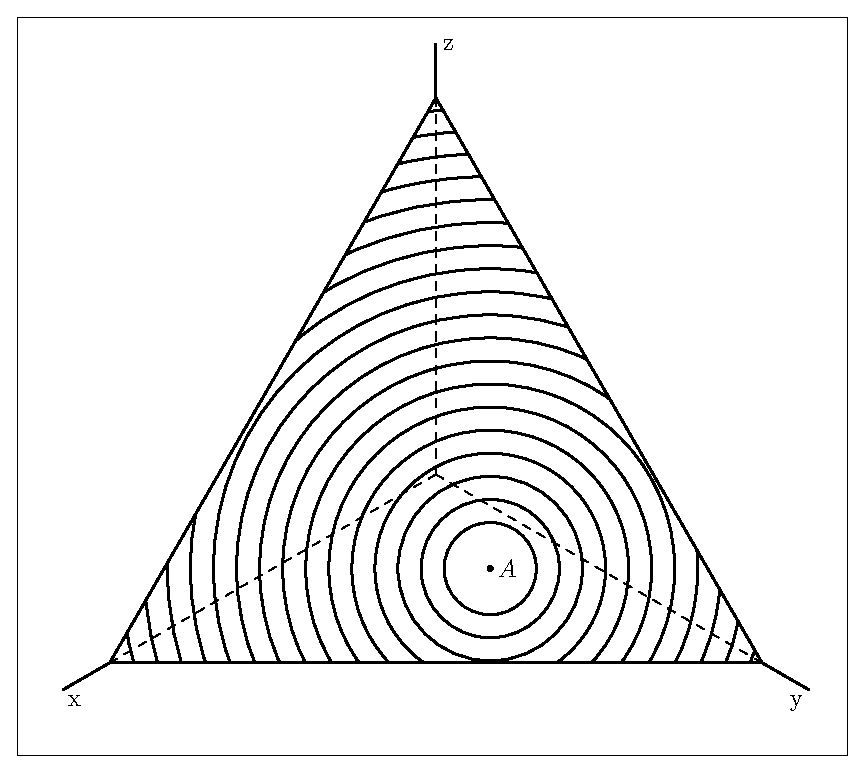
\includegraphics[width=\textwidth]{contourslp.eps}
      \caption{\footnotesize The simplex $\mathbb{S}^{2}$ in
        three-dimensional space $\mathbb{R}^{3}$ with contour lines
        corresponding to the geometry of reason around point $A$ in
        equation (\ref{eq:e6}). Points on the same contour line are
        equidistant from $A$ with respect to the Euclidean metric.
        Compare the contour lines here to figure
        \ref{fig:contoursrj}. Note that this diagram and all the
        following diagrams are frontal views of the simplex.}
      \label{fig:contourslp}
    \end{minipage}
\end{figure}

\begin{figure}[ht!]
    \begin{minipage}[h]{.7\linewidth}
      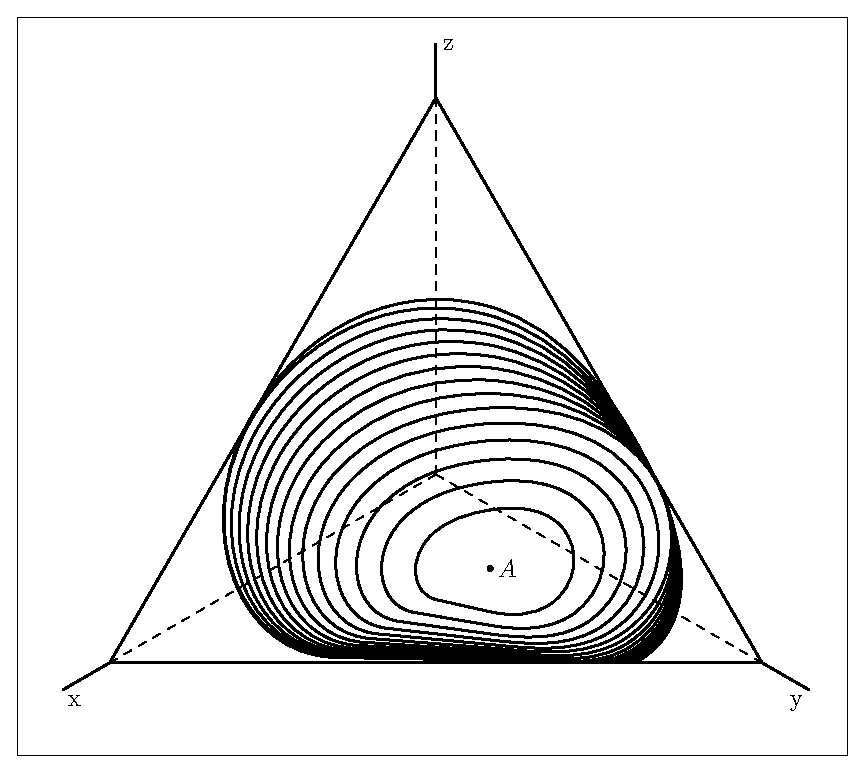
\includegraphics[width=\textwidth]{crj.eps}
      \caption{\footnotesize The simplex $\mathbb{S}^{2}$ with contour
        lines corresponding to information theory around point $A$ in
        equation (\ref{eq:e6}). Points on the same contour line are
        equidistant from $A$ with respect to the Kullback-Leibler
        divergence. The contrast to {\igure}~\ref{fig:contourslp} will
        become clear in much more detail in the body of the chapter.
        Note that the contour lines of the geometry of reason are
        insensitive to the boundaries of the simplex, while the
        contour lines of information theory reflect them. One of the
        main arguments in this chapter is that information theory
        respects epistemic intuitions we have about asymmetry:
        proximity to extreme beliefs with very high or very low
        probability influences the topology that is at the basis of
        updating.}
      \label{fig:contoursrj}
    \end{minipage}
\end{figure}

Epistemic utility in Bayesian epistemology has attracted some
attention in the past few years. Patrick Maher provides a compelling
acceptance-based account of epistemic utility (see
\scite{8}{maher93}{182--207}). Joyce, in \qeins{A Nonpragmatic
  Vindication of Probabilism,} defends probabilism supported by
partial-belief-based epistemic utility rather than the pragmatic
utility common in Dutch-book style arguments (see
\scite{7}{joyce98}{}). For Joyce, norms of gradational accuracy
characterize the epistemic utility approach to partial beliefs,
analogous to norms of truth for full beliefs.

Wallace and Greaves investigate epistemic utility functions along
\qnull{stability} lines and conclude that for everywhere stable
utility functions standard conditioning is optimal, while only
somewhere stable utility functions create problems for maximizing
expected epistemic utility norms (see \scite{7}{greaveswallace06}{};
and \scite{7}{pettigrew13}{}). Richard Pettigrew and Hannes Leitgeb
have published arguments that under certain assumptions probabilism
and standard conditioning (which together give epistemology a distinct
Bayesian flavour) minimize inaccuracy, thereby providing maximal
epistemic utility (see Leitgeb and Pettigrew,
\scite{11}{leitgebpettigrew10i}{} and
\scite{11}{leitgebpettigrew10ii}{}).

Leitgeb and Pettigrew show, given the geometry of reason and other
axioms inspired by Joyce (for example normality and dominance), that
in order to avoid epistemic dilemmas we must commit ourselves to a
Brier score measure of inaccuracy and subsequently to probabilism and
standard conditioning. The Brier score is the mean squared error of a
probabilistic forecast. For example, if we look at 100 days for which
the forecast was 30\% rain and the incidence of rain was 32 days, then
the Brier score is
\begin{equation}
  \label{eq:thahthoo}
  \frac{1}{N}\sum_{i=1}^{N}\left(f_{y}-o_{t}\right)=\frac{1}{100}\left(32\cdot{}(0.3-1)+68\cdot{}(0.3-0)\right)=0.218
\end{equation}
$0$ is a perfect match between forecast and reality in the sense that
the forecaster anticipates every instance of rain with a 100\%
forecast and every instance of no rain with a 0\% forecast.

Jeffrey conditioning (also called probability kinematics) is widely
considered to be a commonsense extension of standard conditioning. On
Leitgeb and Pettigrew's account, using the Brier score, it fails to
provide maximal epistemic utility. Another type of conditioning, which
we will call LP conditioning, takes the place of Jeffrey conditioning.
The failure of Jeffrey conditioning to minimize inaccuracy on the
basis of the geometry of reason casts, by reductio, doubt on the
geometry of reason.

I will show that LP conditioning, which the geometry of reason
entails, fails commonsense expectations that are reasonable to have
for the kind of updating scenario that LP conditioning addresses. To
relate probability distributions to each other geometrically, using
the isomorphism between the set of probability distributions on a
finite event space $W$ with $|W|=n$ and the $n-1$-dimensional simplex
$\mathbb{S}^{n-1}\subset\mathbb{R}^{n}$, is initially an arbitrary
move. Leitgeb and Pettigrew do little to substantiate a link between
the geometry of reason and epistemic utility on a conceptual level. It
is the formal success of the model that makes the geometry of reason
attractive, but the failure of LP conditioning to meet basic
expectations undermines this success.

The question then remains whether we have a plausible candidate to
supplant the geometry of reason. The answer is yes: information theory
provides us with a measure of closeness between probability
distributions on a finite event space that has more conceptual appeal
than the geometry of reason, especially with respect to epistemic
utility---it is intuitively correct to relate coming-to-knowledge to
exchange of information. More persuasive than intuition, however, is
the fact that information theory supports both standard conditioning
(see \scite{7}{williams80}{}) and the extension of standard
conditioning to Jeffrey conditioning (see
subsection~\ref{subsec:ukotooje}), an extension which is on the one
hand intuitive (see \scite{7}{wagner02}{}) and on the other hand
formally continuous with the standard conditioning which Leitgeb and
Pettigrew have worked so hard to vindicate nonpragmatically. LP
conditioning is not continuous with standard conditioning, which is
reflected in one of the expectations that LP conditioning fails to
meet.

\section{Epistemic Utility and the Geometry of Reason}
\label{sec:chuweiyo}

\subsection{Epistemic Utility for Partial Beliefs}
\label{subsec:oochihei}

There is more epistemic virtue for an agent in believing a truth
rather than not believing it and in not believing a falsehood rather
than believing it. Accuracy in full belief epistemology can be
measured by counting four sets, believed truths and falsehoods as well
as unbelieved truths and falsehoods, and somehow relating them to each
other such that epistemic virtue is rewarded and epistemic vice
penalized. Accuracy in partial belief epistemology must take a
different shape since as a \qnull{guess} all partial non-full beliefs
are off the mark so that they need to be appreciated as
\qnull{estimates} instead. Richard Jeffrey distinguishes between
guesses and estimates: a guess fails unless it is on target, whereas
an estimate succeeds depending on how close it is to the target.

The gradational accuracy needed for partial belief epistemology is
reminiscent of verisimilitude and its associated difficulties in the
philosophy of science (see \scite{7}{popper63}{};
\scite{7}{gemes07}{}; and \scite{7}{oddie13}{}). Both Joyce and
Leitgeb/Pettigrew propose axioms for a measure of gradational accuracy
for partial beliefs relying on the geometry of reason, i.e.\ the idea
of geometrical distance between distributions of partial belief
expressed in non-negative real numbers. In Joyce, a metric space for
probability distributions is adopted without much reflection. The
midpoint between two points, for example, which is freely used by
Joyce, assumes symmetry between the end points. The asymmetric
divergence measure that I propose as an alternative to the Euclidean
distance measure has no meaningful concept of a midpoint.

Leitgeb and Pettigrew muse about alternative geometries, especially
non-Euclidean ones. They suspect that these would be based on and in
the end reducible to Euclidean geometry but they do not entertain the
idea that they could drop the requirement of a metric topology
altogether (for the use of non-Euclidean geodesics in statistical
inference see \scite{7}{amari85}{}). Thomas Mormann explicitly warns
against the assumption that the metrics for a geometry of logic is
Euclidean by default, \qeins{All too often, we rely on geometric
  intuitions that are determined by Euclidean prejudices. The geometry
  of logic, however, does not fit the standard Euclidean metrical
  framework} (see \scite{8}{mormann05}{433}; also
\scite{7}{miller84}{}). Mormann concludes in his article
\qeins{Geometry of Logic and Truth Approximation,}

\begin{quotex}
  Logical structures come along with ready-made geometric structures
  that can be used for matters of truth approximation. Admittedly,
  these geometric structures differ from those we are accostumed [sic]
  with, namely, Euclidean ones. Hence, the geometry of logic is not
  Euclidean geometry. This result should not come as a big surprise.
  There is no reason to assume that the conceptual spaces we use for
  representing our theories and their relations have an Euclidean
  structure. On the contrary, this would appear to be an improbable
  coincidence. \scite{3}{mormann05}{453}
\end{quotex}

\subsection{Axioms for Epistemic Utility}
\label{subsec:eichaequ}

Leitgeb and Pettigrew present the following salient axioms (see
\scite{8}{leitgebpettigrew10i}{219}):

\begin{quotex}
  \textbf{Local Normality and Dominance}: If $I$ is a legitimate
  inaccuracy measure, then there is a strictly increasing function
  $f:\mathbb{R}^{+}_{0}\rightarrow\mathbb{R}^{+}_{0}$ such that, for
  any $A\in{}W$, $w\in{}W$, and $x\in\mathbb{R}^{+}_{0}$,
  \begin{equation}
    \label{eq:e4}
    I(A,w,x)=f\left(|\chi_{A}(w)-x|\right).
  \end{equation}
\end{quotex}

\begin{quotex}
  \textbf{Global Normality and Dominance}: If $G$ is a legitimate
  global inaccuracy measure, there is a strictly increasing function
  $g:\mathbb{R}^{+}_{0}\rightarrow\mathbb{R}^{+}_{0}$ such that, for
  all worlds $w$ and belief functions $b\in{}\mbox{Bel}(W)$,
  \begin{equation}
    \label{eq:e5}
  G(w,b)=g\left(\|w-b_{\mbox{{\tiny glo}}}\|\right).
  \end{equation}
\end{quotex}

Similarly to Joyce, these axioms are justified on the basis of
geometry, but this time more explicitly so:

\begin{quotex}
  Normality and Dominance [are] a consequence of taking seriously the
  talk of inaccuracy as \qnull{distance} from the truth, and [they
  endorse] the geometrical picture provided by Euclidean $n$-space as
  the correct clarification of this notion. As explained in section
  3.2, the assumption of this geometrical picture is one of the
  presuppositions of our account, and we do not have much to offer in
  its defense, except for stressing that we would be equally
  interested in studying the consequences of minimizing expected
  inaccuracy in a non-Euclidean framework. But without a doubt,
  starting with the Euclidean case is a natural thing to do.
\end{quotex}

Leitgeb and Pettigrew define two notions, local and global inaccuracy,
and show that one must adopt a Brier score to measure inaccuracy in
order to avoid epistemic dilemmas trying to minimize inaccuracy on
both measures. To give the reader an idea what this looks like in
detail and for purposes of later exposition, I want to provide some of
the formal apparatus. Let $W$ be a set of worlds and $A\subseteq{}W$ a
proposition. Then

\begin{equation}
  \label{eq:linacc}
  I:P(W)\times{}W\times{}\mathbb{R}^{+}_{0}\rightarrow\mathbb{R}^{+}_{0}
\end{equation}

{\noindent}is a measure of local inaccuracy such that $I(A,w,x)$
measures the inaccuracy of the degree of credence $x$ with respect to
$A$ at world $w$. Let $\mbox{Bel}(W)$ be the set of all belief
functions (what we have been calling distributions of partial belief).
Then

\begin{equation}
  \label{eq:ginacc}
  G:W\times\mbox{Bel}(W)\rightarrow\mathbb{R}^{+}_{0}
\end{equation}

{\noindent}is a measure of global inaccuracy of a belief function $b$
at a possible world $w$ such that $G(w,b)$ measures the inaccuracy of
a belief function $b$ at world $w$.

Axioms such as normality and dominance guarantee that the only
legitimate measure of inaccuracy are Brier scores if one wants to
avoid epistemic dilemmas where one receives conflicting advice from
the local and the global measures. For local inaccuracy measures, this
means that there is $\lambda\in\mathbb{R}^{+}$ such that

\begin{equation}
  \label{eq:e1}
  I(A,w,x)=\lambda\left(\chi_{A}(w)-x\right)^{2}
\end{equation}

{\noindent}where $\chi_{A}$ is the characteristic function of $A$. For global
inaccuracy measures, this means that there is $\mu\in\mathbb{R}^{+}$
such that

\begin{equation}
  \label{eq:e2}
  G(w,b)=\mu\|w-b\|^{2}
\end{equation}

where $w$ and $b$ are represented by vectors and $\|u-v\|$ is the
Euclidean distance

\begin{equation}
  \label{eq:e3}
  \sqrt{\sum_{i=1}^{n}\left(u_{i}-v_{i}\right)^{2}}.
\end{equation}

We use (\ref{eq:e1}) to define expected local inaccuracy of degree of
belief $x$ in proposition $A$ by the lights of belief function $b$,
with respect to local inaccuracy measure $I$, and over the set $E$ of
epistemically possible worlds as follows:

\begin{equation}
  \label{eq:eli}
  \mbox{LExp}_{b}(I,A,E,x)=\sum_{w\in{}E}b(\{w\})I(A,w,x)=\sum_{w\in{}E}b(\{w\})\lambda\left(\chi_{A}(w)-x\right)^{2}.
\end{equation}

We use (\ref{eq:e2}) to define expected global inaccuracy of belief
function $b'$ by the lights of belief function $b$, with respect to
global inaccuracy measure $G$, and over the set $E$ of epistemically
possible worlds as follows:

\begin{equation}
  \label{eq:egi}
  \mbox{GExp}_{b}(G,E,b')=\sum_{w\in{}E}b(\{w\})G(w,b')=\sum_{w\in{}E}b(\{w\})\mu\|w-b\|^{2}.
\end{equation}

To give a flavour of how attached the axioms are to the geometry of
reason, here are Joyce's axioms called Weak Convexity and Symmetry,
which he uses to justify probabilism. Note that in terms of notation
$I$ for Joyce is global and related to Leitgeb and Pettigrew's $G$ in
(\ref{eq:ginacc}) rather than $I$ in (\ref{eq:linacc}):

\begin{quotex}
\label{quot:weakconv}
  \textbf{Weak Convexity}: Let $m=(0.5b'+0.5b'')$ be the midpoint of the line
  segment between $b'$ and $b''$. If $I(b',\omega)=I(b'',\omega)$,
  then it will always be the case that $I(b',\omega)\geq{}I(m,\omega)$
  with identity only if $b'=b''$.
\end{quotex}

\begin{quotex}
\label{quot:symmetry}
  \textbf{Symmetry}: If $I(b',\omega)=I(b'',\omega)$, then for any
  $\lambda\in{}[0,1]$ one has\newline
  $I(\lambda{}b'+(1-\lambda)b'',\omega)=I((1-\lambda){}b'+\lambda{}b''),\omega)$.
\end{quotex}

Joyce advocates for these axioms in Euclidean terms, using
justifications such as \qeins{the change in belief involved in going
  from $b'$ to $b''$ has the same direction but a doubly greater
  magnitude than change involved in going from $b'$ to [the midpoint]
  $m$} (see \scite{8}{joyce98}{596}). In section
\ref{subsec:Asymmetry}, I will show that Weak Convexity holds, and
Symmetry does not hold, in \qnull{information geometry,} the topology
generated by the Kullback-Leibler divergence. The term information
geometry is due to Imre Csisz{\'a}r, who considers the
Kullback-Leibler divergence a non-commutative (asymmetric) analogue of
squared Euclidean distance and derives several results that are
intuitive information geometric counterparts of standard results in
Euclidean geometry (see chapter~3 of \scite{7}{csiszarshields04}{}).

\subsection{Expectations for Jeffrey-Type Updating Scenarios}
\label{subsec:vidiedoo}

Leitgeb and Pettigrew's work is continuous with Joyce's work, but
significantly goes beyond it. Joyce wants much weaker assumptions and
would be leery of expected inaccuracies (\ref{eq:eli}) and
(\ref{eq:egi}), as they might presuppose the probabilism that Joyce
wants to justify. Leitgeb and Pettigrew investigate not only whether
probabilism and standard conditioning follow from gradational accuracy
based on the geometry of reason, but also uniform distribution (their
term for the claim of objective Bayesians that there is some principle
of indifference for ignorance priors) and Jeffrey conditioning. They
show that uniform distribution requires additional axioms which are
much less plausible than the ones on the basis of which they derive
probabilism and standard conditioning (see
\scite{8}{leitgebpettigrew10ii}{250f}); and that Jeffrey conditioning
does not fulfill Joyce's Norm of Gradational Accuracy (see
\scite{8}{joyce98}{579}) and therefore violates the pursuit of
epistemic virtue. Leitgeb and Pettigrew provide us with an alternative
method of updating for Jeffrey-type updating scenarios, which I will
call LP conditioning.

\begin{quotex}
  \beispiel{Sherlock Holmes}\label{ex:holmes} Sherlock Holmes
  attributes the following probabilities to the propositions $E_{i}$
  that $k_{i}$ is the culprit in a crime:
  $P(E_{1})=1/3,P(E_{2})=1/2,P(E_{3})=1/6$, where $k_{1}$ is Mr.\ R.,
  $k_{2}$ is Ms.\ S., and $k_{3}$ is Ms.\ T. Then Holmes finds some
  evidence which convinces him that $P'(F^{*})=1/2$, where $F^{*}$ is
  the proposition that the culprit is male and $P$ is relatively prior
  to $P'$. What should be Holmes' updated probability that Ms.\ S. is
  the culprit?
\end{quotex}

% toodeloo
I will look at the recommendations of Jeffrey conditioning and LP
conditioning for {\xample} \ref{ex:holmes} in the next section. For
now note that LP conditioning violates all of the following plausible
expectations in List One\label{page:listone} for an amujus, an
\qnull{alternative method of updating for Jeffrey-type updating
  scenarios.} This is List One:

\begin{itemize}
\item \textsc{continuity} An amujus ought to be continuous with
  standard conditioning as a limiting case.
\item \textsc{regularity} An amujus ought not to assign a posterior
  probability of $0$ to an event which has a positive prior
  probability and about which the intervening evidence says nothing
  except that a strictly weaker event has a positive posterior
  probability.
\item \textsc{levinstein} An amujus ought not to give \qeins{extremely
    unattractive} results in a Levinstein scenario (see
  \scite{7}{levinstein12}{}, which not only articulates this failed
  expectation for LP conditioning, but also the previous two).
\item \textsc{invariance} An amujus ought to be partition invariant.
\item \textsc{expansibility} An amujus ought to be insensitive to an
  expansion of the event space by zero-probability events.
\item \textsc{confirmation} An amujus ought to align with intuitions
  we have about degrees of confirmation.
\item \textsc{horizon} An amujus ought to exhibit the horizon effect
  which makes probability distributions which are nearer to extreme
  probability distributions appear to be closer to each other than
  they really are.
\end{itemize}

Jeffrey conditioning and LP conditioning are both an amujus based on a
concept of quantitative difference between probability distributions
measured as a function on the isomorphic manifold (in our case, an
$n-1$-dimensional simplex). Evidence appears in the form of a
constraint on acceptable probability distributions and the closest
acceptable probability to the orginal (relatively prior) probability
distribution is chosen as its successor. Here is List
Two\label{page:listtwo}, a list of reasonable expectations one may
have toward this concept of quantitative difference (we call it a
distance function for the geometry of reason and a divergence for
information theory). Let $d(p,q)$ express this concept mathematically.

\begin{itemize}
\item \textsc{triangularity} The concept obeys the triangle
  inequality. If there is an intermediate probability distribution, it
  will not make the difference smaller: $d(p,r)\leq{}d(p,q)+d(q,r)$.
  Buying a pair of shoes is not going to be more expensive than buying
  the two shoes individually.
\item \textsc{collinear horizon} This expecation is just a more
  technical restatement of the \textsc{horizon} expectation in the
  previous list. If $p,p',q,q'$ are collinear with the centre of the
  simplex $m$ (whose coordinates are $m_{i}=1/n$ for all $i$) and an
  arbitrary but fixed boundary point $\xi\in\partial\mathbb{S}^{n-1}$
  and $p,p',q,q'$ are all between $m$ and $\xi$ with
  $\|p'-p\|=\|q'-q\|$ where $p$ is strictly closest to $m$, then
  $|d(p,p')|<|d(q,q')|$. For an illustration of this expectation see
  {\igure}~\ref{fig:conditions}. The absolute value is added as a
  feature to accommodate degree of confirmation functions in
  subsection~\ref{subsec:ooraisoh}, which may be negative.
\item \textsc{transitivity of asymmetry} An ordered pair $(p,q)$ of
  simplex points associated with probability distributions is
  asymmetrically negative, positive, or balanced, so either
  $d(p,q)-d(q,p)<0$ or $d(p,q)-d(q,p)>0$ or $d(p,q)-d(q,p)=0$. If
  $(p,q)$ and $(q,r)$ are asymmetrically positive, $(p,r)$ ought not
  to be asymmetrically negative. Think of a bicycle route map with
  different locations at varying altitudes. If it takes 20 minutes to
  get from $A$ to $B$ but only 15 minutes to get from $B$ to $A$ then
  $(A,B)$ is asymmetrically positive. If $(A,B)$ and $(B,C)$ are
  asymmetrically positive, then $(A,C)$ ought not to be asymmetrically
  negative.
\end{itemize}

\begin{figure}[ht!]
    \begin{minipage}[h]{.7\linewidth}
      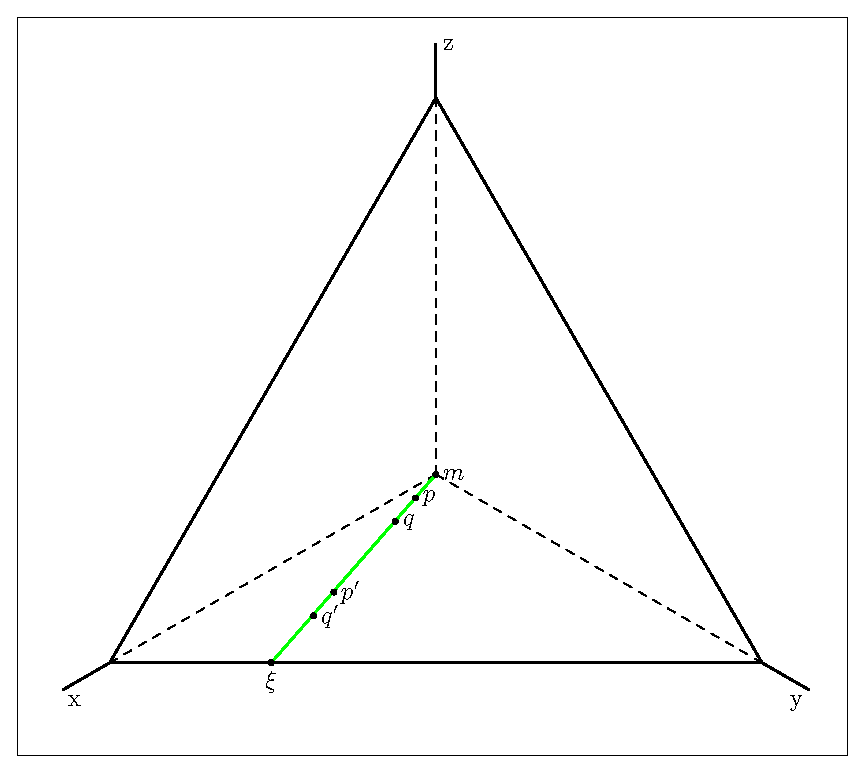
\includegraphics[width=\textwidth]{horeff.eps}
      \caption{\footnotesize An illustrations of conditions (i)--(iii)
        for \textsc{collinear horizon} in List Two. $p,p'$ and $q,q'$
        must be equidistant and collinear with $m$ and $\xi$. If
        $q,q'$ is more peripheral than $p,p'$, then \textsc{collinear
          horizon} requires that $|d(p,p')|<|d(q,q')|$.}
      \label{fig:conditions}
    \end{minipage}
\end{figure}

While the Kullback-Leibler divergence of information theory fulfills
all the expectations of List One, save \textsc{horizon}, it fails all
the expectations in List Two. Obversely, the Euclidean distance of the
geometry of reason fulfills all the expectations of List Two, save
\textsc{collinear horizon}, and fails all the expectations in List
One. Information theory has its own axiomatic approach to justifying
probabilism and standard conditioning (see
\scite{7}{shorejohnson80}{}). Information theory provides a
justification for Jeffrey conditioning and generalizes it (see
subsection~\ref{subsec:ukotooje}). All of these virtues stand in
contrast to the violations of the expectations in List Two. The rest
of this chapter fills in the details of these violations both for the
geometry of reason and information theory, with the conclusion that
the case for the geometry of reason is hopeless while the case for
information theory is now a major challenge for future research
projects.

\section{Geometry of Reason versus Information Theory}
\label{sec:shahseid}

Here is a simple example where the distance of geometry and the
divergence of information theory differ. With this difference in mind,
I will show how LP conditioning fails the expectations outlined in
List One (see page \pageref{page:listone}). Consider the following three
points in three-dimensional space:

\begin{equation}
  \label{eq:e6}
    a=\left(\frac{1}{3},\frac{1}{2},\frac{1}{6}\right) \hspace{.5in}
    b=\left(\frac{1}{2},\frac{3}{8},\frac{1}{8}\right)  \hspace{.5in}
    c=\left(\frac{1}{2},\frac{5}{12},\frac{1}{12}\right)
\end{equation}

All three are elements of the simplex $\mathbb{S}^{2}$: their
coordinates add up to $1$. Thus they represent probability
distributions $A,B,C$ over a partition of the event space into three
events. The Kullback-Leibler divergence and Euclidean distance give
different re\-commendations with respect to proximity. Note that the
Kullback-Leibler divergence defined in (\ref{eq:xaingouw}) is always
positive as a consequence of Gibbs' inequality, irrespective of
dimension, (see \scite{7}{mackay03}{}, sections 2.6 and 2.7). The
Euclidean distance $\|B-A\|$ is defined as in equation (\ref{eq:e3}).
What is remarkable about the three points in (\ref{eq:e6}) is that

\begin{equation}
  \label{eq:e8}
  \|C-A\|\approx{}0.204<\|B-A\|\approx{}0.212
\end{equation}

and

\begin{equation}
  \label{eq:e9}
  D_{\mbox{\tiny KL}}(B,A)\approx{}0.0589<D_{\mbox{\tiny KL}}(C,A)\approx{}0.069.
\end{equation}

{\noindent}Assuming the global inaccuracy measure presented in (\ref{eq:e2}) and
$E=W$ (all possible worlds are epistemically accessible),

\begin{equation}
  \label{eq:e8a}
  \mbox{GExp}_{A}(C)\approx{}0.653<\mbox{GExp}_{A}(B)\approx{}0.656.
\end{equation}

\begin{figure}[ht!]
    \begin{minipage}[h]{.7\linewidth}
      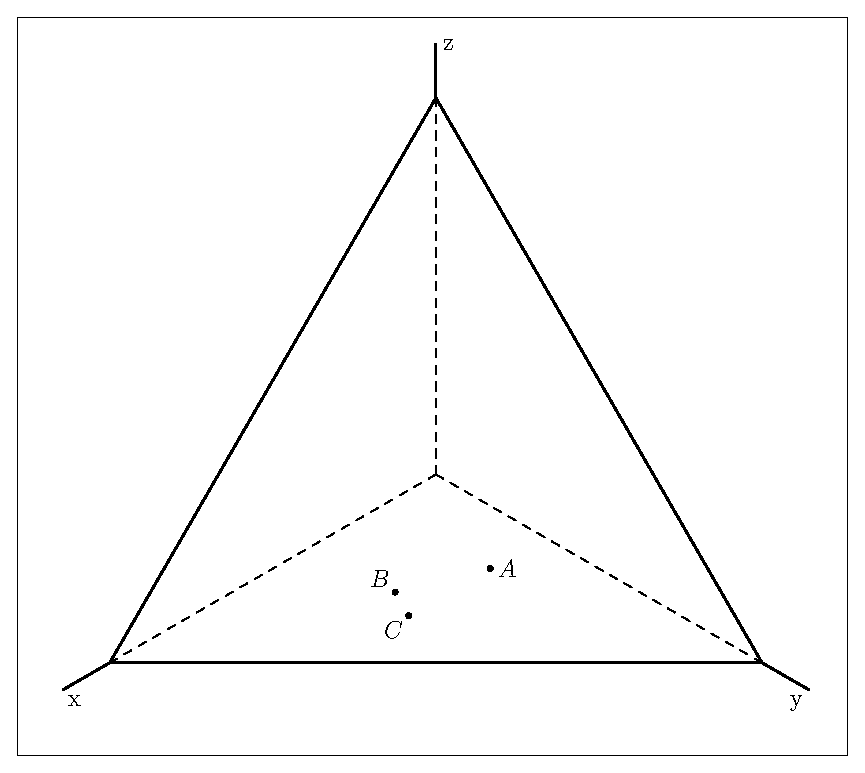
\includegraphics[width=\textwidth]{threepoints.eps}
      \caption{\footnotesize The simplex $\mathbb{S}^{2}$ in
        three-dimensional space $\mathbb{R}^{3}$ with points $a,b,c$
        as in equation (\ref{eq:e6}) representing probability
        distributions $A,B,C$. Note that geometrically speaking $C$ is
        closer to $A$ than $B$ is. Using the Kullback-Leibler
        divergence, however, $B$ is closer to $A$ than $C$ is. The
        same case modeled with statistical parameters is illustrated
        in {\igure}s~\ref{fig:finmod} and~\ref{fig:finmoe}.}
      \label{fig:threepoints}
    \end{minipage}
\end{figure}

Global inaccuracy reflects the Euclidean proximity relation, not the
re\-commendation of information theory. If $A$ corresponds to my prior
and my evidence is such that I must change the first coordinate to
$1/2$ (as in {\xample}~\ref{ex:holmes}) and nothing stronger, then
information theory via the Kullback-Leibler divergence re\-commends
the posterior corresponding to $B$; and the geometry of reason as
expounded in Leitgeb and Pettigrew recommends the posterior
corresponding to $C$. There are several things going on here that need
some explanation.

\subsection{Evaluating Partial Beliefs in Light of Others}
\label{subsec:aichavag}

We note that for Leitgeb and Pettigrew, expected global inaccuracy of
$b'$ is always evaluated by the lights of another partial belief
distribution $b$. This may sound counterintuitive. Should we not
evaluate $b'$ by its own lights? It is part of a larger Bayesian
commitment that partial belief distributions are not created ex
nihilo. They can also not be evaluated for inaccuracy ex nihilo.
Leitgeb and Pettigrew say very little about this, but it appears that
there is a deeper problem here with the flow of diachronic updating.
The classic Bayesian picture is one of moving from a relatively prior
probability distribution to a posterior distribution (distinguish
relatively prior probability distributions, which precede posterior
probability distributions in updating, from absolutely prior
probability distributions, which are ignorance priors in the sense
that they are not the resulting posteriors of previous updating). This
is nicely captured by standard conditioning, Bayes' formula, and
updating on the basis of information theory (Jeffrey conditioning,
principle of maximum entropy).

The geometry of reason and notions of accuracy based on it sit
uncomfortably with this idea of flow, as the suggestion is that
partial belief distributions are evaluated on their accuracy without
reference to prior probability distributions---why should the
accuracy or epistemic virtue of a posterior probability distribution
depend on a prior probability distribution which has already been
debunked by the evidence? I agree with Leitgeb and Pettigrew that
there is no alternative here but to evaluate the posterior by the
lights of the prior. Not doing so would saddle us with Carnap's
Straight Rule, where priors are dismissed as irrelevant (see
\scite{8}{carnap52}{40ff}). Yet we shall note that a justification of
evaluating a belief function's accuracy by the lights of another
belief function is a lot less persuasive than the way Bayesians and
information theory integrate prior distributions into forming
posterior distributions by virtue of an asymmetric flow of
information (see also \scite{7}{shogenji12}{}, who makes a strong case
for the influence of prior probabilities on epistemic justification).

\subsection{LP conditioning and Jeffrey Conditioning}
\label{subsec:meexughi}

I want to outline how Leitgeb and Pettigrew arrive at posterior
probability distributions in Jeffrey-type updating scenarios. I will
call their method LP conditioning.

\begin{quotex}
  \beispiel{Abstract Holmes}\label{ex:abstract} Consider a possibility
  space $W=E_{1}\cup{}E_{2}\cup{}E_{3}$ (the $E_{i}$ are sets of
  states which are pairwise disjoint and whose union is $W$) and a
  partition $\mathcal{F}$ of $W$ such that
  $\mathcal{F}=\{F^{*},F^{**}\}=\{E_{1},E_{2}\cup{}E_{3}\}$.
\end{quotex}

Let $P$ be the prior probability function on $W$ and $P'$ the
posterior. I will keep the notation informal to make this simple, not
mathematically precise. Jeffrey-type updating scenarios give us new
information on the posterior probabilities of partitions such as
$\mathcal{F}$. In {\xample} \ref{ex:abstract}, let

\begin{equation}
  \label{eq:priors}
  \begin{array}{rcl}
    P(E_{1})&=&1/3 \\
    P(E_{2})&=&1/2 \\
    P(E_{3})&=&1/6
  \end{array}
\end{equation}

{\noindent}and the new evidence constrain $P'$ such that
$P'(F^{*})=1/2=P'(F^{**})$.

Jeffrey conditioning works on the following intuition, which elsewhere
I have called Jeffrey's updating principle \textsc{jup} (see also
\scite{7}{wagner02}{}). The posterior probabilities
conditional on the partition elements equal the prior probabilities
conditional on the partition elements since we have no information in
the evidence that they should have changed. Hence,

\begin{align}
  \label{eq:jc}
  &P'_{\mbox{\tiny JC}}(E_{i})&=&P'(E_{i}|F^{*})P'(F^{*})+P'(E_{i}|F^{**})P'(F^{**})\notag \\
  &&=&P(E_{i}|F^{*})P'(F^{*})+P(E_{i}|F^{**})P'(F^{**})
\end{align}

Jeffrey conditioning is controversial (for an introduction to Jeffrey
conditioning see \scite{7}{jeffrey65}{}; for its statistical and
formal properties see \scite{7}{diaconiszabell82}{}; for a pragmatic
vindication of Jeffrey conditioning see \scite{7}{armendt80}{}, and
\scite{7}{skyrms86}{}; for criticism see
\scite{7}{howsonfranklin94}{}). Information theory, however, supports
Jeffrey conditioning. Leitgeb and Pettigrew show that Jeffrey
conditioning does not in general pick out the minimally inaccurate
posterior probability distribution. If the geometry of reason as
presented in Leitgeb and Pettigrew is sound, this would constitute a
powerful criticism of Jeffrey conditioning. Leitgeb and Pettigrew
introduce an alternative to Jeffrey conditioning, which we have called
LP conditioning. It proceeds as follows for {\xample} \ref{ex:abstract}
and in general provides the minimally inaccurate posterior probability
distribution in Jeffrey-type updating scenarios.

Solve the following two equations for $x$ and $y$:

\begin{equation}
  \label{eq:lpce}
  \begin{array}{rcl}
    P(E_{1})+x&=&P'(F^{*}) \\
    P(E_{2})+y+P(E_{3})+y&=&P'(F^{**})
  \end{array}
\end{equation}

{\noindent}and then set

\begin{equation}
  \label{eq:lpcf}
  \begin{array}{rcl}
    P'_{\mbox{\tiny LP}}(E_{1})&=&P(E_{1})+x \\
    P'_{\mbox{\tiny LP}}(E_{2})&=&P(E_{2})+y \\
    P'_{\mbox{\tiny LP}}(E_{3})&=&P(E_{3})+y
  \end{array}
\end{equation}

For the more formal and more general account see
\scite{8}{leitgebpettigrew10ii}{254}. The results for {\xample}
\ref{ex:abstract} are:

\begin{equation}
  \label{eq:lpcres}
  \begin{array}{rcl}
    P'_{\mbox{\tiny LP}}(E_{1})&=&1/2 \\
    P'_{\mbox{\tiny LP}}(E_{2})&=&5/12 \\
    P'_{\mbox{\tiny LP}}(E_{3})&=&1/12
  \end{array}
\end{equation}

{\noindent}Compare these results to the results of Jeffrey conditioning:

\begin{equation}
  \label{eq:jcres}
  \begin{array}{rcl}
    P'_{\mbox{\tiny JC}}(E_{1})&=&1/2 \\
    P'_{\mbox{\tiny JC}}(E_{2})&=&3/8 \\
    P'_{\mbox{\tiny JC}}(E_{3})&=&1/8
  \end{array}
\end{equation}

{\noindent}Note that (\ref{eq:priors}), (\ref{eq:jcres}), and (\ref{eq:lpcres})
correspond to $A,B,C$ in (\ref{eq:e6}). 

\subsection{Triangulating LP and Jeffrey Conditioning}
\label{subsec:ieseiwoh}

There is an interesting connection between LP conditioning and Jeffrey
conditioning as updating methods. Let $B$ be on the zero-sum line
between $A$ and $C$ if and only if

\begin{equation}
\label{eq:jooziphu}
d(A,C)=d(A,B)+d(B,C)
\end{equation}

{\noindent}where $d$ is the difference measure we are using, so $d(A,B)=\|B-A\|$
for the geometry of reason and $d(A,B)=D_{\mbox{\tiny KL}}(B,A)$ for
information geometry. For the geometry of reason (and Euclidean
geometry), the zero-sum line between two probability distributions is
just what we intuitively think of as a straight line: in Cartesian
coordinates, $B$ is on the zero-sum line strictly between $A$ and $C$
if and only if for some $\vartheta\in(0,1)$,
$b_{i}=\vartheta{}a_{i}+(1-\vartheta)c_{i}$ and $i=1,\ldots,n$.

What the zero-sum line looks like for information theory is
illustrated in {\igure}~\ref{fig:eugoohue}. The reason for the oddity is
that the Kullback-Leibler divergence does not obey
\textsc{triangularity}, an issue that we will address in detail in
subsection~\ref{subsec:triangularity}). Call $B$ a zero-sum point
between $A$ and $C$ if (\ref{eq:jooziphu}) holds true. For the
geometry of reason, the zero-sum points are simply the points on the
straight line between $A$ and $C$. For information geometry, the
zero-sum poins are the boundary points of the set where you can take a
shortcut by making a detour, i.e.\ all points for which
$d(A,B)+d(B,C)<d(A,C)$.

\begin{figure}[ht!]
    \begin{minipage}[h]{.7\linewidth}
      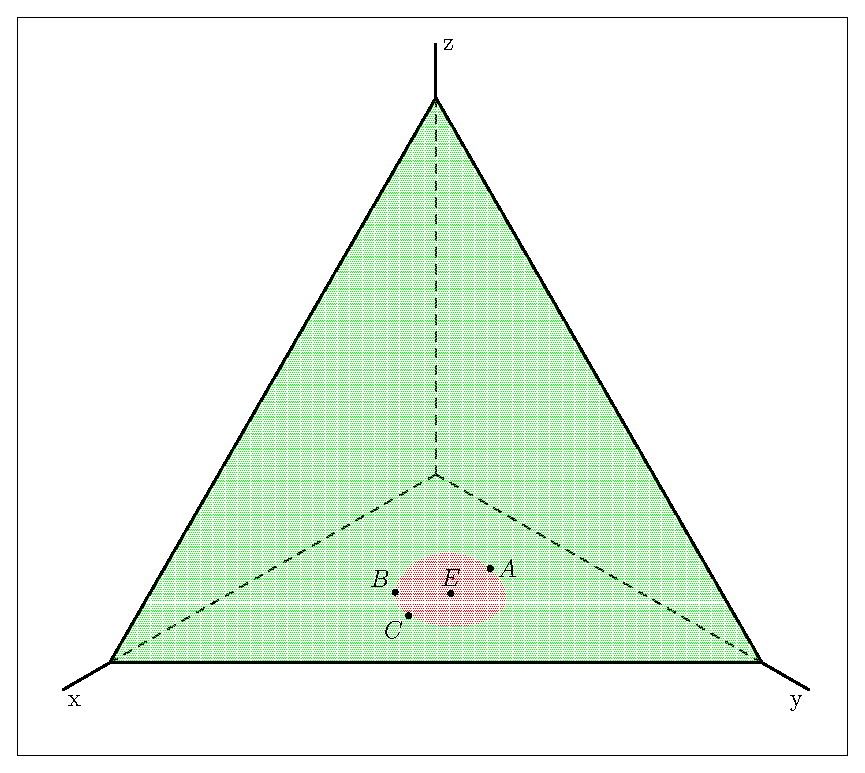
\includegraphics[width=\textwidth]{dreieck.eps}
      \caption{\footnotesize The zero-sum line between $A$ and $C$ is
        the boundary line between the green area, where the triangle
        inequality holds, and the red area, where the triangle
        inequality is violated. The posterior probability distribution
        $B$ recommended by Jeffrey conditioning always lies on the
        zero-sum line between the prior $A$ and the LP posterior $C$,
        as per equation (\ref{eq:ocidocho}). $E$ is the point in the
        red area where the triangle inequality is most efficiently
        violated.}
      \label{fig:eugoohue}
\end{minipage}
\end{figure}

Remarkably, if $A$ represents a relatively prior probability
distribution and $C$ the posterior probability distribution
recommended by LP conditioning, the posterior probability distribution
recommended by Jeffrey conditioning is always a zero-sum point with
respect to the Kullback-Leibler divergence:

\begin{equation}
  \label{eq:ocidocho}
  D_{\mbox{\tiny KL}}(C,A)=D_{\mbox{\tiny KL}}(B,A)+D_{\mbox{\tiny KL}}(C,B)
\end{equation}

Informationally speaking, if you go from $A$ to $C$, you can just as
well go from $A$ to $B$ and then from $B$ to $C$. This does not mean
that we can conceive of information geometry the way we would conceive
of non-Euclidean geometry, where it is also possible to travel faster
on what from a Euclidean perspective looks like a detour. For in
information geometry, you can travel faster on what from the
perspective of information theory (!) looks like a detour, i.e.\ the
triangle inequality does not hold. 

To prove equation (\ref{eq:ocidocho}) in the case $n=3$ (assuming that
LP conditioning does not \qnull{fall off the edge} as in case (b) in
\scite{8}{leitgebpettigrew10ii}{253}) note that all three points
(prior, point recommended by Jeffrey conditioning, point recommended
by LP conditioning) can be expressed using three variables:

\begin{equation}
  \label{eq:reejeiru}
  \begin{array}{rcl}
    A&=&\left(1-\alpha,\beta,\alpha-\beta\right) \\
     && \\
    B&=&\left(1-\gamma,\frac{\gamma\beta}{\alpha},\frac{\gamma(\alpha-\beta)}{\alpha}\right) \\
     && \\
    C&=&\left(1-\gamma,\beta+\frac{1}{2}(\gamma-\alpha),\alpha-\beta+\frac{1}{2}(\gamma-\alpha)\right)
  \end{array}
\end{equation}

The rest is basic algebra using the definition of the Kullback-Leibler
divergence in (\ref{eq:xaingouw}). To prove the claim for arbitrary
$n$ one simply generalizes (\ref{eq:reejeiru}). It is a handy
corollary of (\ref{eq:ocidocho}) that whenever $(A,B)$ and $(B,C)$
violate \textsc{transitivity of asymmetry} then

\begin{equation}
  \label{eq:saithain}
  D_{\mbox{\tiny KL}}(A,C)>D_{\mbox{\tiny KL}}(B,C)+D_{\mbox{\tiny KL}}(A,B)
\end{equation}

{\noindent}in violation of \textsc{triangularity}. This way we will not have to
go hunting for an example to demonstrate the violation of
\textsc{triangularity}. $A,B,C$ of (\ref{eq:e6}) fulfill all the
conditions for (\ref{eq:saithain}) and therefore violate
\textsc{triangularity}.

It is an interesting question to wonder which point $E$ violates the
triangle inequality most efficiently so that

\begin{equation}
  \label{eq:eaghaidu}
D_{\mbox{\tiny KL}}(E,C)+D_{\mbox{\tiny KL}}(A,E)  
\end{equation}

{\noindent}is minimal. Let $e=(e_{1},\ldots,e_{n})$ represent $E$ in
$\mathbb{S}^{n-1}$. Use the Lagrange Multiplier method to find the
Lagrangian

\begin{equation}
  \label{eq:eiweehee}
  \mathcal{L}(e,\lambda)=\sum_{i=1}^{n}e_{i}\log\frac{e_{i}}{a_{i}}+\sum_{i=1}^{n}c_{i}\log\frac{c_{i}}{e_{i}}+\lambda\left(\sum_{i=1}^{n}e_{i}-1\right)
\end{equation}

{\noindent}The Lagrange Multiplier method gives us

\begin{equation}
  \label{eq:nainguji}
  \frac{\partial\mathcal{L}}{\partial{}e_{k}}=\log\frac{e_{k}}{a_{k}}+1-\frac{r}{q}+\lambda=0\mbox{ for each }k=1,{\ldots},n.
\end{equation}

{\noindent}Manipulate this equation to yield

\begin{equation}
  \label{eq:ohjoogoh}
  \frac{c_{k}}{e_{k}}\exp\left(\frac{c_{k}}{e_{k}}\right)=\frac{c_{k}}{a_{k}}\exp(1+\lambda).
\end{equation}

{\noindent}To solve (\ref{eq:ohjoogoh}), use the Lambert W function

\begin{equation}
  \label{eq:ouquuzoh}
  e_{k}=\frac{c_{k}}{W\left(\frac{c_{k}}{a_{k}}\exp(1+\lambda)\right)}.
\end{equation}

{\noindent}Choose $\lambda$ to fulfill the constraint $\sum{}e_{i}=1$. The
result for the discrete case accords with Ovidiu Calin and Constantin
Udriste's result for the continuous case (see equation 4.7.9 in
\scite{8}{calinudriste14}{127}). Numerically, for $A$ and $C$ as
defined in equation (\ref{eq:e6}),

\begin{equation}
  \label{eq:aemaujei}
  E=(0.415,0.462,0.123).
\end{equation}

{\noindent}This is subtly different from the midpoint $m_{i}=0.5a_{i}+0.5c_{i}$
(if we were minimizing
$D_{\mbox{\tiny KL}}(A,E)+D_{\mbox{\tiny KL}}(C,E)$, the solution
would be the midpoint). I do not know whether $A,E,C$ are collinear
(see {\igure}~\ref{fig:eugoohue} for illustration).

\section{Expectations for the Geometry of Reason}
\label{sec:ooyaekoo}

This section provides more detail for the expectations in List One
(see page \pageref{page:listone}) and shows how LP conditioning
violates them.

\subsection{Continuity}
\label{subsec:thaoyahc}

LP conditioning violates \textsc{continuity} because standard
conditioning gives a different recommendation than a parallel sequence
of Jeffrey-type updating scenarios which get arbitrarily close to
standard event observation. This is especially troubling considering
how important the case for standard conditioning is to Leitgeb and
Pettigrew.

To illustrate a \textsc{continuity} violation, consider the case where
Sherlock Holmes reduces his credence that the culprit was male to
$\varepsilon_{n}=1/n$ for $n=4,5,\ldots$. The sequence
$\varepsilon_{n}$ is not meant to reflect a case where Sherlock Holmes
becomes successively more certain that the culprit was female. It is
meant to reflect countably many parallel scenarios which only differ
by the degree to which Sherlock Holmes is sure that the culprit was
female. These parallel scenarios give rise to a parallel sequence (as
opposed to a successive sequence) of updated probabilities
$P'_{\mbox{\tiny LP}}(F^{**})$ and another sequence of updated
probabilities $P'_{\mbox{\tiny JC}}(F^{**})$ ($F^{**}$ is the
proposition that the culprit is female). As $n\rightarrow\infty$, both
of these sequences go to one.

Straightforward conditionalization on the evidence that \qnull{the
  culprit is female} gives us 

\begin{equation}
  \label{eq:sherlockcontsc}
  \begin{array}{rcl}
  P'_{\mbox{\tiny SC}}(E_{1})&=&0\\
  P'_{\mbox{\tiny SC}}(E_{2})&=&3/4\\
  P'_{\mbox{\tiny SC}}(E_{3})&=&1/4.
\end{array}
\end{equation}

{\noindent}Letting $n\rightarrow\infty$ for Jeffrey conditioning yields

\begin{equation}
  \label{eq:sherlockcontjc}
  \begin{array}{rcccl}
  P'_{\mbox{\tiny JC}}(E_{1})&=&1/n&\rightarrow&0\\
  P'_{\mbox{\tiny JC}}(E_{2})&=&3(n-1)/4n&\rightarrow&3/4\\
  P'_{\mbox{\tiny JC}}(E_{3})&=&(n-1)/4n&\rightarrow&1/4,
\end{array}
\end{equation}

{\noindent}whereas letting $n\rightarrow\infty$ for LP conditioning yields

\begin{equation}
  \label{eq:sherlockcontlp}
  \begin{array}{rcccl}
  P'_{\mbox{\tiny LP}}(E_{1})&=&1/n&\rightarrow&0\\
  % this is mine, further down is Paul's 
  % P'_{\mbox{\tiny LP}}(E_{2})&=&(4n-1)/6n&\rightarrow&2/3\\
  % P'_{\mbox{\tiny LP}}(E_{3})&=&(2n-1)/6n&\rightarrow&1/3.
  P'_{\mbox{\tiny LP}}(E_{2})&=&(4n-3)/6n&\rightarrow&2/3\\
  P'_{\mbox{\tiny LP}}(E_{3})&=&(2n-5)/6n&\rightarrow&1/3.
\end{array}
\end{equation}

{\noindent}LP conditioning violates \textsc{continuity}.

\subsection{Regularity}
\label{subsec:shoedaic}

LP conditioning violates \textsc{regularity} because formerly positive
probabilities can be reduced to $0$ even though the new information in
the Jeffrey-type updating scenario makes no such requirements (as is
usually the case for standard conditioning). Ironically, Jeffrey-type
updating scenarios are meant to be a better reflection of real-life
updating because they avoid extreme probabilities. 

The violation becomes serious if we are already sympathetic to an
infor\-ma\-tion-based account: the amount of information required to
turn a non-extreme probability into one that is extreme ($0$ or $1$)
is infinite. Whereas the geometry of reason considers extreme
probabilities to be easily accessible by non-extreme probabilities
under new information (much like a marble rolling off a table or a
bowling ball heading for the gutter), information theory envisions
extreme probabilities more like an event horizon. The nearer you are
to the extreme probabilities, the more information you need to move
on. For an observer, the horizon is never reached.

\begin{quotex}
  \beispiel{Regularity Holmes}\label{ex:regularity} Everything is as
  in {\xample} \ref{ex:holmes}, except that Sherlock Holmes becomes
  confident to a degree of $2/3$ that Mr.\ R is the culprit and
  updates his relatively prior probability distribution in
  (\ref{eq:priors}).
\end{quotex}

{\noindent}Then his posterior probabilities look as follows:

\begin{equation}
  \label{eq:sherlockposteriorjcreg}
  \begin{array}{rcl}
  P'_{\mbox{\tiny JC}}(E_{1})&=&2/3\\
  P'_{\mbox{\tiny JC}}(E_{2})&=&1/4\\
  P'_{\mbox{\tiny JC}}(E_{3})&=&1/12
\end{array}
\end{equation}

\begin{equation}
  \label{eq:sherlockposteriorlpreg}
  \begin{array}{rcl}
  P'_{\mbox{\tiny LP}}(E_{1})&=&2/3\\
  P'_{\mbox{\tiny LP}}(E_{2})&=&1/3\\
  P'_{\mbox{\tiny LP}}(E_{3})&=&0
\end{array}
\end{equation}

{\noindent}With LP conditioning, Sherlock Holmes' subjective
probability that Ms.\ T is the culprit in {\xample}
\ref{ex:regularity} has been reduced to zero. No finite amount of
information could bring Ms.\ T back into consideration as a culprit in
this crime, and Sherlock Holmes should be willing to bet any amount of
money against a penny that she is not the culprit---even though his
evidence is nothing more than an increase in the probability that Mr.\
R is the culprit.

LP conditioning violates \textsc{regularity}.

\subsection{Levinstein}
\label{subsec:tohcahye}

LP conditioning violates \textsc{levinstein} because of \qeins{the
  potentially dramatic effect [LP conditioning] can have on the
  likelihood ratios between different propositions}
\scite{3}{levinstein12}{419}. Consider Benjamin Levinstein's example:

\begin{quotex}
  \beispiel{Levinstein's Ghost}\label{ex:levinstein} There is a car
  behind an opaque door, which you are almost sure is blue but which
  you know might be red. You are almost certain of materialism, but
  you admit that there's some minute possibility that ghosts exist.
  Now the opaque door is opened, and the lighting is fairly good. You
  are quite surprised at your sensory input: your new credence that
  the car is red is very high.
\end{quotex}

Jeffrey conditioning leads to no change in opinion about ghosts. Under
LP conditioning, however, seeing the car raises the probability that
there are ghosts to an astonishing 47\%, given Levinstein's reasonable
priors. Levinstein proposes a logarithmic inaccuracy measure as a
remedy to avoid violation of \textsc{levinstein}. As a special case of
applying a Levinstein-type logarithmic inaccuracy measure, information
theory does not violate \textsc{levinstein}.

\subsection{Invariance}
\label{subsec:afaisiug}

LP conditioning violates \textsc{invariance} because two agents who
have identical credences with respect to a partition of the event
space may disagree about this partition after LP conditioning, even
when the Jeffrey-type updating scenario provides no new information
about the more finely grained partitions on which the two agents
disagree. 

\begin{quotex}
  \beispiel{Jane Marple}\label{ex:marple} Jane Marple is on the same
  case as Sherlock Holmes in {\xample} \ref{ex:holmes} and arrives at
  the same relatively prior probability distribution as Sherlock
  Holmes (we will call Jane Marple's relatively prior probability
  distribution $Q$ and her posterior probability distribution $Q'$).
  Jane Marple, however, has a more finely grained probability
  assignment than Sherlock Holmes and distinguishes between the case
  where Ms.\ S went to boarding school with her, of which she has a
  vague memory, and the case where Ms.\ S did not and the vague memory
  is only about a fleeting resemblance of Ms.\ S with another boarding
  school mate. Whether or not Ms.\ S went to boarding school with Jane
  Marple is completely beside the point with respect to the crime, and
  Jane Marple considers the possibilities equiprobable whether or not
  Ms.\ S went to boarding school with her.
\end{quotex}

{\noindent}Let $E_{2}\equiv{}E_{2}^{*}\vee{}E_{2}^{**}$, where $E_{2}^{*}$ is the
proposition that Ms.\ S is the culprit and she went to boarding school
with Jane Marple and $E_{2}^{**}$ is the proposition that Ms.\ S is
the culprit and she did not go to boarding school with Jane Marple.
Then

\begin{equation}
  \label{eq:marpleprior}
  \begin{array}{rcl}
  Q(E_{1})&=&1/3\\
  Q(E_{2}^{*})&=&1/4\\
  Q(E_{2}^{**})&=&1/4\\
  Q(E_{3})&=&1/6.
\end{array}
\end{equation}

{\noindent}Now note that while Sherlock Holmes and Jane Marple agree on the
relevant facts of the criminal case (who is the culprit?) in their
posterior probabilities if they use Jeffrey conditioning,

\begin{equation}
  \label{eq:sherlockposteriorjc}
  \begin{array}{rcl}
  P'_{\mbox{\tiny JC}}(E_{1})&=&1/2\\
  P'_{\mbox{\tiny JC}}(E_{2})&=&3/8\\
  P'_{\mbox{\tiny JC}}(E_{3})&=&1/8
\end{array}
\end{equation}

\begin{equation}
  \label{eq:marpleposteriorjc}
  \begin{array}{rcl}
  Q'_{\mbox{\tiny JC}}(E_{1})&=&1/2\\
  Q'_{\mbox{\tiny JC}}(E_{2}^{*})&=&3/16\\
  Q'_{\mbox{\tiny JC}}(E_{2}^{**})&=&3/16\\
  Q'_{\mbox{\tiny JC}}(E_{3})&=&1/8
\end{array}
\end{equation}

{\noindent}they do not agree if they use LP conditioning,

\begin{equation}
  \label{eq:sherlockposteriorlp}
  \begin{array}{rcl}
  P'_{\mbox{\tiny LP}}(E_{1})&=&1/2\\
  P'_{\mbox{\tiny LP}}(E_{2})&=&5/12\\
  P'_{\mbox{\tiny LP}}(E_{3})&=&1/12
\end{array}
\end{equation}

\begin{equation}
  \label{eq:marpleposteriorlp}
  \begin{array}{rcl}
  Q'_{\mbox{\tiny LP}}(E_{1})&=&1/2\\
  Q'_{\mbox{\tiny LP}}(E_{2}^{*})&=&7/36\\
  Q'_{\mbox{\tiny LP}}(E_{2}^{**})&=&7/36\\
  Q'_{\mbox{\tiny LP}}(E_{3})&=&1/9.
\end{array}
\end{equation}

{\noindent}LP conditioning violates \textsc{invariance}.

\subsection{Expansibility}
\label{Expansibility}

One particular problem with the lack of invariance for LP conditioning
is how zero-probability events should be included in the list of prior
probabilities that determines the value of the posterior
probabilities. Consider

\begin{equation}
  \label{eq:reginvone}
  \begin{array}{rcl}
  P(X_{1})&=&0\\
  P(X_{2})&=&0.3\\
  P(X_{3})&=&0.6\\
  P(X_{4})&=&0.1\\
\end{array}
\end{equation}

{\noindent}That $P(X_{1})=0$ may be a consequence of standard conditioning in a
previous step. Now the agent learns that $P'(X_{3}\vee{}X_{4})=0.5$.
Should the agent update on the list presented in (\ref{eq:reginvone})
or on the following list:

\begin{equation}
  \label{eq:reginvtwo}
  \begin{array}{rcl}
  P(X_{2})&=&0.3\\
  P(X_{3})&=&0.6\\
  P(X_{4})&=&0.1\\
\end{array}
\end{equation}

{\noindent}Whether you update on (\ref{eq:reginvone}) or (\ref{eq:reginvtwo})
makes no difference to Jeffrey conditioning, but due to the lack of
invariance it makes a difference to LP conditioning, so the geometry
of reason needs to find a principled way to specify the appropriate
prior probabilities. The only non-arbitrary way to do this is either
to include or to exclude all zero probability events on the list. This
strategy, however, sounds ill-advised unless one signs on to a
stronger version of \textsc{regularity} and requires that only a fixed
set of events can have zero probabilities (such as logical
contradictions), but then the geometry of reason ends up in the
catch-22 of LP conditioning running afoul of \textsc{regularity}.

LP conditioning violates \textsc{expansibility}.

\subsection{Horizon}
\label{subsec:uurohkei}

\begin{quotex}
  \beispiel{Undergraduate Complaint}\label{ex:complaint} An
  undergraduate student complains to the department head that the
  professor will not reconsider an 89\% grade (which misses an A+ by
  one percent) when reconsideration was given to other students with a
  67\% grade (which misses a B- by one percent).
\end{quotex}

Intuitions may diverge, but the professor's reasoning is as follows.
To improve a 60\% paper by ten percent is easily accomplished: having
your roommate check your grammar, your spelling, and your line of
argument will sometimes do the trick. It is incomparably more
difficult to improve an 85\% paper by ten percent: it may take doing a
PhD to turn a student who writes the former into a student who writes
the latter. A maiore ad minus, the step from 89\% to 90\% is greater
than the step from 67\% to 68\%.

Another example for the horizon effect is George Schlesinger's
comparison between the risk of a commercial airplane crash and the
risk of a military glider landing in enemy territory.

\begin{quotex}
  \beispiel{Airplane Gliders}\label{ex:schlesinger} Compare two
  scenarios. In the first, an airplane which is considered safe
  (probability of crashing is $1/10^{9}$) goes through an
  inspection where a mechanical problem is found which increases
  the probability of a crash to $1/100$. In the second, military
  gliders land behind enemy lines, where their risk of perishing
  is 26\%. A slight change in weather pattern increases this risk
  to 27\%. \scite{3}{schlesinger95}{211}
\end{quotex}

For an interesting instance of the horizon effect in asymmetric
multi-dimen\-sional scaling see \scite{7}{chinoshiraiwa93}{}, section~3,
where Naohito Chino and Kenichi Shiraiwa describe as one of the
properties of their Hilbert space models of asymmetry how \qeins{the
  similarity between the pair of objects located far from the centroid
  of objects, say, the origin, is greater than that located near the
  origin, even if their distances are the same} (42).

I claim that an amujus ought to fulfill the requirements of the
horizon effect: it ought to be more difficult to update as
probabilities become more extreme (or less middling). I have
formalized this requirement in List Two (see page
\pageref{page:listtwo}). It is trivial that the geometry of reason
does not fulfill it. Information theory fails as well, which gives the
horizon effect its prominent place in both lists. The way information
theory fails, however, is quite different. Near the boundary of
$\mathbb{S}^{n-1}$, information theory reflects the horizon effect
just as our expectation requires. The problem is near the centre,
where some equidistant points are more divergent the closer they are
to the middle. I will give an example and more explanation in
subsection~\ref{subsec:colhor}.

In the next section, I will closely tie the issue of the horizon
effect to confirmation. The two main candidates for quantitative
measures of relevance confirmation disagree on precisely this issue.
Whether you, the reader, will accept the horizon requirement may
depend on what your view is on degree of confirmation theory.

\subsection{Confirmation}
\label{subsec:ooraisoh}

The geometry of reason thinks about the comparison of probability
distributions in terms of distance. Information theory thinks about
the comparison along the lines of information loss when one
distribution is used to encode a message rather than the other
distribution. One way to test these approaches is to ask how well they
align with a third approach to such a comparison: degree of
confirmation. Our main concern is the horizon effect of the previous
subsection. Which approaches to degree of confirmation theory reflect
it, and how do these approaches correspond to the disagreements
between information theory and the geometry of reason?

There is, of course, a relevant difference between the aims of the
epistemic utility approach to updating and the aims of degree of
confirmation theory. The former investigates norms to which a rational
agent conforms in her pursuit of epistemic virtue. The latter seeks to
establish qualitative and quantitative measures of impact that
evidence has on a hypothesis. Both, however, (I will restrict my
attention here to quantitative degree of confirmation theory) attend
to the probability of an event, which degree of confirmation theory
customarily calls $h$ for hypothesis, before and after the rational
agent processes another event, customarily called $e$ for evidence,
i.e.\ $x=P(h|k)$ and $y=P(h|e,k)$ ($k$ is background information).

For perspectives on the link between confirmation and information see
\scite{8}{shogenji12}{37f}; \scite{7}{crupitentori14}{}; and
\scite{7}{milne14}{}, section~4. Vincenzo Crupi and Katya Tentori
suggest that there is a \qeins{parallelism between confirmation and
  information search [which] can serve as a valuable heuristic for
  theoretical work} \scite{3}{crupitentori14}{89}. 

In degree of confirmation theory, incremental confirmation is
distinguished from absolute confirmation in the following sense. Let
$h$ be the presence of a very rare disease and $e$ a test result such
that $y>>x$ but $y<1-y$. Then, absolutely speaking, $e$ disconfirms
$h$ (for Rudolf Carnap, absolute confirmation involves sending $y$
above a threshold $r$ which must be greater than or equal to $0.5$).
Absolute confirmation is not the subject of this section. I will
exclusively discuss incremental confirmation (also called relevance
confirmation, just as absolute confirmation is sometimes called
firmness confirmation) where $y>x$ implies (incremental) confirmation,
$y<x$ implies (incremental) disconfirmation, and $y=x$ implies the
lack of both. The difference is illustrated in
{\igure}~\ref{fig:doconf}.

All proposed measures of quantitative, incremental degree of
confirmation considered here are a function of $x$ and $y$. Dependence
of incremental confirmation on only $x$ and $y$ is not trivial, as
$P(e|k)$ and $P(e|h,k)$ cannot be expressed using only $x$ and $y$
(for a case why dependence should be on only $x$ and $y$ see
\scite{8}{atkinson12}{50}, with an irrelevant conjunction argument;
and \scite{8}{milne14}{254}, with a continuity argument). David
Christensen's measure $P(h|e,k)-P(h|\urcorner{}e,k)$ (see
\scite{8}{christensen99}{449}) and Robert Nozick's
$P(e|h,k)-P(e|\urcorner{}h,k)$ (see \scite{8}{nozick81}{252}) are not
only dependent on $x$ and $y$, but also on $P(e|k)$, which makes them
vulnerable to Atkinson's and Milne's worries just cited.

Consider the following six contenders for a quantitative, incremental
degree of confirmation function, dependent on only $x$ and $y$. They
are based on, in a brief slogan, (i) difference of conditional
probabilities, (ii) ratio of conditional probabilities, (iii)
difference of odds, (iv) ratio of likelihoods, (v) Gaifman's treatment
of Hempel's raven paradox, and (vi) conservation of contrapositivity
and commutativity. Logarithms throughout this dissertation are assumed
to be the natural logarithm in order to facilitate easy
differentiation, although generally a particular choice of base
(greater than one) does not make a relevant difference.

% zahThe2a
\begin{equation}
  \label{eq:relevance}
  \begin{array}{lrcl}
    \mbox{(i) } & M_{P}(x,y)&=&y-x \\
                &&& \\
    \mbox{(ii) } & R_{P}(x,y)&=&\displaystyle\log\frac{y}{x} \\
                &&& \\
    \mbox{(iii) } & J_{P}(x,y)&=&\displaystyle\frac{y}{1-y}-\frac{x}{1-x} \\
                &&& \\
    \mbox{(iv) } & L_{P}(x,y)&=&\displaystyle\log\frac{y(1-x)}{x(1-y)} \\
                &&& \\
    \mbox{(v) } & G_{P}(x,y)&=&\displaystyle\log\frac{1-x}{1-y} \\
                &&& \\
    \mbox{(vi) } & Z_{P}(x,y)&=&\left\{
                                 \begin{array}{cl}
                                   \displaystyle\frac{y-x}{1-x}&\mbox{if }y\geq{}x \\
                                   \displaystyle\frac{y-x}{x}&\mbox{if }y<x
                                 \end{array}\right.
  \end{array}
\end{equation}

{\noindent}$M_{P}$ is defended by \scite{7}{carnap62}{}; \scite{7}{earman92}{};
\scite{7}{rosenkrantz94}{}. $R_{P}$ is defended by
\scite{7}{keynes21}{}; \scite{7}{milne96}{}; \scite{7}{shogenji12}{}.
$J_{P}$ is defended by \scite{7}{festa99}{}. $L_{P}$ is defended by
\scite{7}{good50}{}; \scite{7}{good83}{}, chapter~14;
\scite{7}{fitelson06}{}; \scite{7}{zalabardo09}{}. $G_{P}$ is defended
by \scite{8}{gaifman79}{120}, without the logarithm (I added it to
make $G_{P}$ more comparable to the other functions). $Z_{P}$ is
defended by \scite{7}{crupietal07}{}. For more literature supporting
the various measures consult footnote 1 in
\scite{8}{fitelson01}{S124}; and an older survey of options in
\scite{7}{kyburg83}{}.

To compare how these degree of confirmation measures align with the
concept of difference between probability distributions for the
purpose of updating it is best to look at derivatives as they reflect
the rate of change from the middle to the extremes. This is how we
capture the horizon effect requirement for two dimensions. One
important difference between degree of confirmation theory and
updating is that the former is concerned with a hypothesis and its
negation whereas the latter considers all sorts of domains for the
probability distribution (in this chapter, I have restricted myself to
a finite outcome space). As far as the analogy between degree of
confirmation theory on the one hand and updating on the other hand is
concerned, we only need to look at the two-dimensional case.

To discriminate between candidates (i)--(vi), I am setting up three
criteria (complementing many others in the literature). Let $D(x,y)$
be the generic expression for the degree of confirmation function.
Call this List Three\label{page:listthree}.

\begin{itemize}
\item \textsc{additivity} A theory can be confirmed piecemeal. Whether
  the evidence is split up into two or more components or left in one
  piece is irrelevant to the amount of confirmation it confers.
  Formally, $D(x,z)=D(x,y)+D(y,z)$. Note that this is not the usual
  triangle inequality because we are in two dimensions.
\item \textsc{skew-antisymmetry} It does not matter whether $h$ or
  $\urcorner{}h$ is in view. Confirmation and disconfirmation are
  commensurable. Formally, $D(x,y)=-D(1-x,1-y)$. A surprising number
  of candidates fail this requirement, and the requirement is not
  common in the literature (see, however, the second clause in Milne's
  fourth desideratum in \scite{10}{milne96}{21}). In defence of this
  requirement consider {\xample} \ref{ex:ieyohjah} below.
  $d_{1}>{}d_{2}$ may have a negative impact on the latter scientist's
  grant application, even though the inequality may solely be due to a
  failure to fulfill skew-antisymmetry.
\item \textsc{confirmation horizon} An account of degree of
  confirmation must exhibit the horizon effect as in List One and List
  Two, except more simply in two dimensions. Formally, the functions
  $\partial{}D_{\varepsilon}^{+}/\partial{}x$ must be strictly
  positive and the functions
  $\partial{}D_{\varepsilon}^{-}/\partial{}x$ must be strictly
  negative for all $\varepsilon\in{}(-1/2,1/2)$. These functions are
  defined in (\ref{eq:defdhpos}) and (\ref{eq:defdhneg}), and I prove
  in appendix \ref{app:horform} that the requirement to keep them
  strictly positive/neg\-ative is equivalent to the horizon effect as
  described formally in List Two (see page \pageref{page:listtwo}).
\end{itemize}

\begin{quotex}
  \beispiel{Grant Adjudication I}\label{ex:ieyohjah} Two scientists
  compete for grant money. Professor X presents an experiment
  conferring degree of confirmation $d_{1}$ on a hypothesis, if
  successful; Professor Y presents an experiment conferring degree of
  disconfirmation $-d_{2}$ on the negation of the same hypothesis, if
  unsuccessful. (For the relevance of quantitative confirmation
  measures to the evaluation of scientific projects see
  \scite{8}{salmon75}{11}.)
\end{quotex}

The functions for the horizon effect are defined as follows. Let
$\varepsilon\in{}(-1/2,1/2)$ be fixed. Recall that $D(x,y)$ is the
generic expression for a confirmation function measuring the degree of
confirmation that a posterior $y=P(h|e,k)$ bestows on a hypothesis for
which the prior is $x=P(h|k)$. $\varepsilon$ is the difference $y-x$.
For $\varepsilon>0$,

\begin{equation}
  \begin{array}{lrcl}
  D_{\varepsilon}^{-}:(0,\frac{1}{2}-\varepsilon)\rightarrow{}\mathbb{R} & D_{\varepsilon}^{-}(x)&=&|D(x,x+\varepsilon)| \\
  D_{\varepsilon}^{+}:(\frac{1}{2},1-\varepsilon)\rightarrow{}\mathbb{R} & D_{\varepsilon}^{+}(x)&=&|D(x,x+\varepsilon)| \\
  \end{array}
  \label{eq:defdhpos}
\end{equation}

{\noindent}For $\varepsilon<0$,

\begin{equation}
  \begin{array}{lrcl}
  D_{\varepsilon}^{-}:(-\varepsilon,\frac{1}{2})\rightarrow{}\mathbb{R} & D_{\varepsilon}^{-}(x)&=&|D(x,x+\varepsilon)| \\
  D_{\varepsilon}^{+}:(\frac{1}{2}-\varepsilon,1)\rightarrow{}\mathbb{R} & D_{\varepsilon}^{+}(x)&=&|D(x,x+\varepsilon)| \\
  \end{array}
  \label{eq:defdhneg}
\end{equation}

The rate of change for the different quantitative measures of degree
of confirmation can be observed in {\igure}~\ref{fig:doconf}. The pass
and fail verdicts in the table below are evident from
{\igure}~\ref{fig:doconf} and the table of derivatives provided in
appendix~\ref{app:horform}. Only $J_{P},L_{P}$ and $Z_{P}$ fulfill the
horizon requirement.

\begin{figure}[ht!]
    \begin{minipage}[h]{\linewidth}
      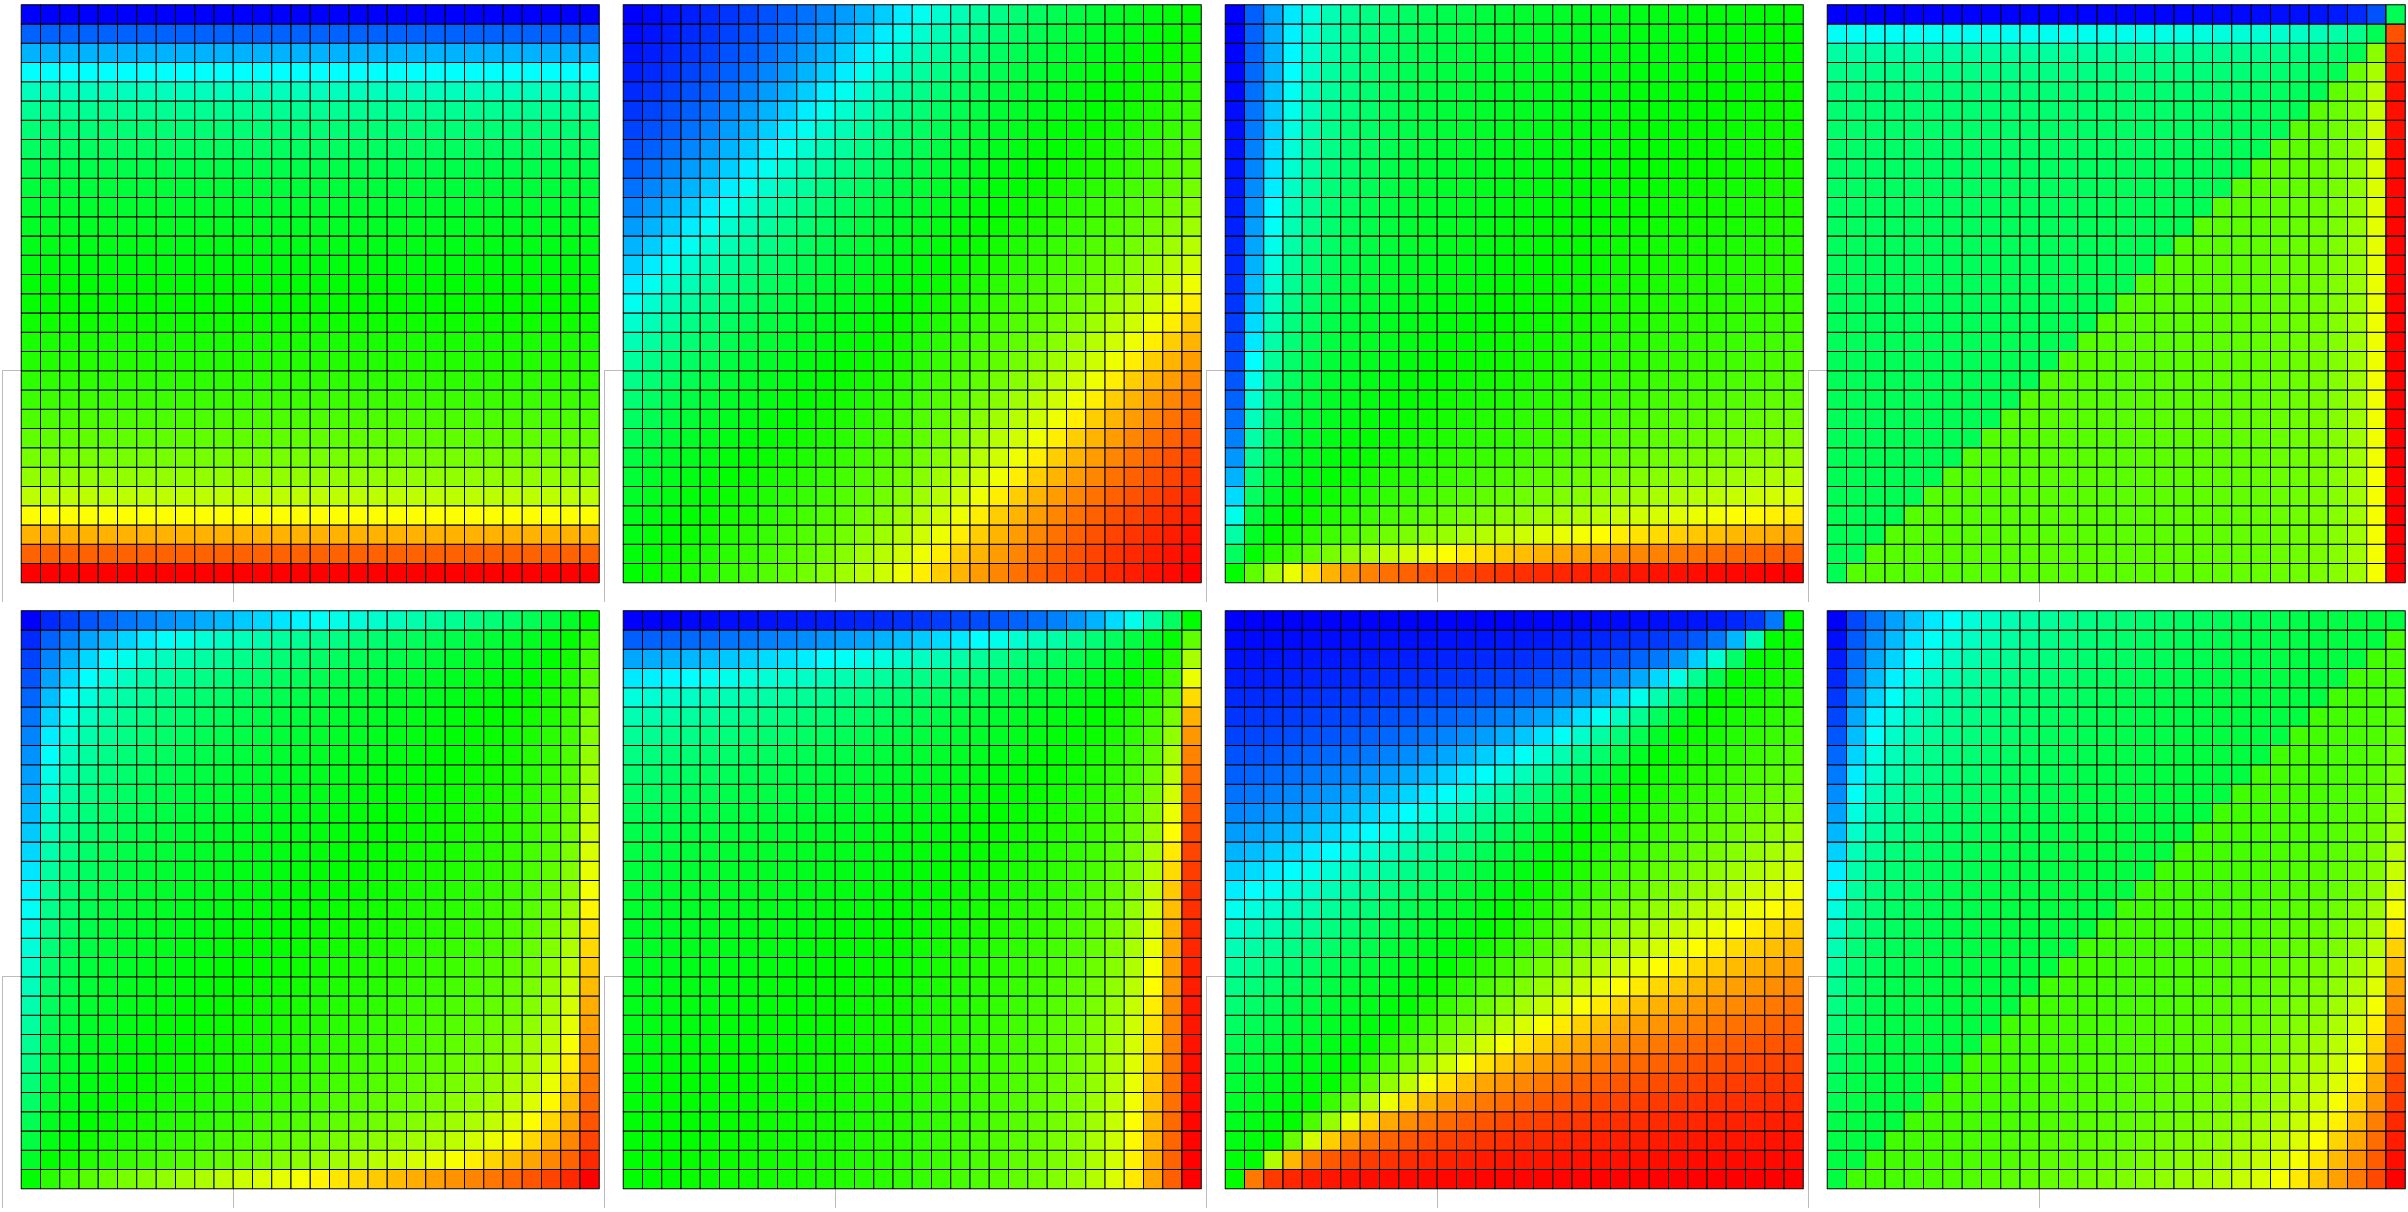
\includegraphics[width=\textwidth]{confirmation-FMRJLGZI.png}
      \caption{\footnotesize Illustration for the six degree of
        confirmation candidates plus Carnap's firmness confirmation
        and the Kullback-Leibler divergence. The top row, from left to
        right, illustrates FMRJ, the bottom row LGZI. \qnull{F} stands
        for Carnap's firmness confirmation measure
        $F_{P}(x,y)=\log(y/(1-y))$. \qnull{M} stands for candidate
        (i), $M_{P}(x,y)$ in (\ref{eq:relevance}), the other letters
        correspond to the other candidates (ii)-(v). \qnull{I} stands
        for the Kullback-Leibler divergence multiplied by the sign
        function of $y-x$ to mimic a quantitative measure of
        confirmation. For all the squares, the colour reflects the
        degree of confirmation with $x$ on the $x$-axis and $y$ on the
        $y$-axis, all between $0$ and $1$. The origin of the square's
        coordinate system is in the bottom left corner. Blue signifies
        strong confirmation, red signifies strong disconfirmation, and
        green signifies the scale between them. Perfect green is
        $x=y$. $G_{P}$ looks like it might pass the horizon
        requirement, but the derivative reveals that it fails
        \textsc{confirmation horizon} (see appendix
        \ref{app:horform}).}
      \label{fig:doconf}
\end{minipage}
\end{figure}

\begin{tabular}{|l|l|l|l|}\hline
  \emph{Candidate} & \emph{Triangularity} & \emph{Skew-Antisymmetry} & \emph{Confirmation Horizon} \\ \hline
  $M_{P}$ & pass & pass & fail \\ \hline
  $R_{P}$ & pass & fail & fail \\ \hline
  $J_{P}$ & pass & fail & pass \\ \hline
  $L_{P}$ & pass & pass & pass \\ \hline
  $G_{P}$ & pass & fail & fail \\ \hline
  $Z_{P}$ & fail & pass & pass \\ \hline
\end{tabular}

\medskip

The table makes clear that only $L_{P}$ passes all three tests. I am
not making a strong independent case for $L_{P}$ here, especially
against $M_{P}$, which is the most likely hero of the geometry of
reason. This has been done elsewhere (for example in
\scite{7}{schlesinger95}{}, where $L_{P}$ and $M_{P}$ are compared to
each other in their performance given some intuitive examples; Elliott
Sober presents the counterargument in \scite{7}{sober94}{}). The
argumentative force of this subsection appeals to those who are
already sympathetic to $L_{P}$. Adherents of $M_{P}$ will hopefully
find other items on List One (see page \pageref{page:listone})
persuasive and reject the geometry of reason, in which case they may
come back to this subsection and re-evaluate their commitment to
$M_{P}$.

\begin{quotex}
  \beispiel{Grant Adjudication II}\label{ex:idaboogi} Two scientists
  compete for grant money. Professor X presents an experiment that
  will increase the probability of a hypothesis from $98\%$ to $99\%$,
  if successful. Professor Y presents an experiment that will increase
  the probability of a hypothesis from $1\%$ to $2\%$, if successful.
\end{quotex}

All else being equal, Professor Y should receive the grant money. If
her experiment is more successful, it will arguably make more of a
difference. This example illustrates that the analogy between degree
of confirmation and updating remains tenuous, since for degree of
confirmation theory the consensus on intuitions is far inferior to the
updating case. If, for example, the confirmation function is
anti-symmetric and $D(x,y)-D(y,x)$ is zero (for $M_{P}$ and $L_{P}$,
for example), then together with skew-antisymmetry this means that
degree of confirmation is equal for Professor X and Professor Y.
Despite its three passes in the above table, $L_{P}$ fails here.

Based on Roberto Festa's $J_{P}$, Professor X's prospective degree of
confirmation is 5000 times larger than Professor Y's, but Festa in
particular insists \qeins{that there is no universally applicable
  $P$-incremental $c$-measure, and that the appropriateness of a
  $P$-incremental $c$-measure is highly context-dependent}
\scite{3}{festa99}{67}. $R_{P}$ and $Z_{P}$ appear to be sensitive to
{\xample} \ref{ex:idaboogi}. The Kullback-Leibler divergence gives us
the right result as well, where the degree of confirmation for going
from 1\% to 2\% is $3.91\cdot{}10^{-3}$ compared to
$3.12\cdot{}10^{-3}$ for going from 98\% to 99\%, but the
Kullback-Leibler divergence is not a serious degree of confirmation
candidate. It fulfills \textsc{skew-antisymmetry} and
\textsc{confirmation horizon}, but not \textsc{additivity} (see
subsection~\ref{subsec:triangularity}).

Intuitions easily diverge here. Christensen may be correct when he
says, \qeins{perhaps the controversy between difference and
  ratio-based positive relevance models of quantitative confirmation
  reflects a natural indeterminateness in the basic notion of
  \qnull{how much} one thing supports another}
\scite{3}{christensen99}{460}. Pluralists allow therefore for
\qeins{distinct, complementary notions of evidential support}
\scite{3}{hajekjoyce08}{123}. I am sym\-path\-etic towards this
indeterminateness in degree of confirmation theory, but not when it
comes to updating (see the full employment theorem in section
\ref{sec:shutepae}).

This subsection assumes that despite these problems with the strength
of the analogy, degree of confirmation and updating are sufficiently
similar to be helpful in associating options with each other and
letting the arguments in each other's favour and disfavour
cross-pollinate. As an aside, Christensen's $S$-support given by
evidence $E$ is stable over Jeffrey conditioning on
$[E,\urcorner{}E]$; LP-conditioning is not (see
\scite{8}{christensen99}{451}). This may serve as another argument
from degree of confirmation theory in favour of information theory
(which supports Jeffrey conditioning) against the geometry of reason
(which supports LP conditioning).

\section{Expectations for Information Theory}
\label{sec:expinfth}

Asymmetry is the central feature of the difference concept that
information theory proposes for the purpose of updating between finite
probability distributions. In information theory, the information loss
differs depending on whether one uses probability distribution $P$ to
encode a message distributed according to probability distribution
$Q$, or whether one uses probability distribution $Q$ to encode a
message distributed according to probability distribution $P$. This
asymmetry may very well carry over into the epistemic realm. Updating
from one probability distribution, for example, which has $P(X)=x>0$
to $P'(X)=0$ is common. It is called standard conditioning. Going in
the opposite direction, however, from $P(X)=0$ to $P'(X)=x'>0$ is
controversial and unusual.

The Kullback-Leibler divergence, which is the most promising concept
of difference for probability distributions in information theory and
the one which gives us Bayesian standard conditioning as well as
Jeffrey conditioning, is non-commutative and may provide the kind of
asymmetry required to reflect epistemic asymmetry. However, it also
violates \textsc{triangularity}, \textsc{collinear horizon}, and
\textsc{transitivity of asymmetry}. The task of this section is to
show how serious these violations are.

%}}}

\subsection{Triangularity}
\label{subsec:triangularity}

As mentioned at the end of subsection~\ref{subsec:ieseiwoh}, the three
points $A,B,C$ in (\ref{eq:e6}) violate \textsc{triangularity} as in
(\ref{eq:saithain}):

\begin{equation}
  \label{eq:yohliimo}
  D_{\mbox{\tiny KL}}(A,C)>D_{\mbox{\tiny KL}}(B,C)+D_{\mbox{\tiny KL}}(A,B).
\end{equation}

{\noindent}This is counterintuitive on a number of levels, some of which I have
already hinted at in illustration: taking a shortcut while making a
detour; buying a pair of shoes for more money than buying the shoes
individually. 

Information theory, however, does not only violate
\textsc{triangularity}. It violates it in a particularly egregious
way. Consider any distinct two points $x$ and $z$ on
$\mathbb{S}^{n-1}$ with coordinates $x_{i}$ and $z_{i}$
($1\leq{}i\leq{}n$). For simplicity, let us write
$\delta(x,z)=D_{\mbox{\tiny KL}}(z,x)$. Then, for any
$\vartheta\in{}(0,1)$ and an intermediate point $y$ with coordinates
$y_{i}=\vartheta{}x_{i}+(1-\vartheta)z_{i}$, the following inequality
holds true:

\begin{equation}
  \label{eq:aiphedau}
  \delta(x,z)>\delta\left(x,y\right)+\delta\left(y,z\right).
\end{equation}

{\noindent}I will prove this in a moment, but here is a disturbing consequence:
think about an ever more finely grained sequence of partitions
$y^{j}$, $j\in\mathbb{N}$, of the line segment from $x$ to $z$ with
$y^{jk}$ as dividing points. I will spare you defining these
partitions, but note that any dividing point $y^{j_{0}k}$ will also be a
dividing point in the more finely grained partitions $y^{jk}$ with
$j\geq{}j_{0}$. Then define the sequence

\begin{equation}
  \label{eq:queireiw}
  T_{j}=\sum_{k}\delta\left(y^{jk},y^{j(k+1)}\right)
\end{equation}

{\noindent}such that the sum has as many summands as there are dividing points
for $j$, plus one (for example, two dividing points divide the line
segment into three possibly unequal thirds). If $\delta$ were the
Euclidean distance norm, $T_{j}$ would be constant and would equal
$\|z-x\|$. Zeno's arrow moves happily along from $x$ to $z$, no matter
how many stops it makes on the way. Not so for information theory and
the Kullback-Leibler divergence. According to (\ref{eq:aiphedau}), any
stop along the way reduces the sum of divergences.

$T_{j}$ is a strictly decreasing sequence (does it go to zero? -- I do
not know, but if yes, it would add to the poignancy of this
violation). The more stops you make along the way, the closer you
bring together $x$ and $z$.

For the proof of (\ref{eq:aiphedau}), it is straightforward to see
that (\ref{eq:aiphedau}) is equivalent to

\begin{equation}
  \label{eq:eiquotoh}
  \sum_{i=1}^{n}(z_{i}-x_{i})\log\frac{\vartheta{}x_{i}+(1-\vartheta)z_{i}}{x_{i}}>0.
\end{equation}

{\noindent}Now we use the following trick. Expand the right hand side to

\begin{equation}
  \label{eq:xiechuth}
  \sum_{i=1}^{n}\left(z_{i}+\frac{\vartheta}{1-\vartheta}x_{i}-\frac{\vartheta}{1-\vartheta}x_{i}-x_{i}\right)\log\frac{\frac{1}{1-\vartheta}\left(\vartheta{}x_{i}+(1-\vartheta)z_{i}\right)}{\frac{1}{1-\vartheta}x_{i}}>0.
\end{equation}

{\noindent}(\ref{eq:xiechuth}) is clearly equivalent to (\ref{eq:eiquotoh}). It
is also equivalent to

\begin{equation}
  \label{eq:ohrohshi}
  \sum_{i=1}^{n}\left(z_{i}+\frac{\vartheta}{1-\vartheta}x_{i}\right)\log\frac{z_{i}+\frac{\vartheta}{1-\vartheta}x_{i}}{\frac{1}{1-\vartheta}x_{i}}+
  \sum_{i=1}^{n}\frac{1}{1-\vartheta}x_{i}\log\frac{\frac{1}{1-\vartheta}x_{i}}{z_{i}+\frac{\vartheta}{1-\vartheta}x_{i}}>0,
\end{equation}

{\noindent}which is true by Gibbs' inequality.
% (see \scite{7}{mackay03}{}, section~2.6 and 2.7). 

%{{{

\subsection{Collinear Horizon}
\label{subsec:colhor}

There are two intuitions at work that need to be balanced: on the one
hand, the geometry of reason is characterized by simplicity, and the
lack of curvature near extreme probabilities may be a price worth
paying; on the other hand, simple examples such as those adduced by
Schlesinger make a persuasive case for curvature.

Information theory is characterized by a very complicated
\qnull{semi-quasimetric} (the attribute \qnull{quasi} is due to its
non-commutativity, the attribute \qnull{semi} to its violation of the
triangle inequality). One of its initial appeals is that it performs
well with respect to the horizon requirement near the boundary of the
simplex, which is also the location of Schlesinger's examples. It is
not trivial, however, to articulate what the horizon requirement
really demands.

\textsc{collinear horizon} in List Two seeks to set up the requirement
as weakly as possible, only demanding that points collinear with the
centre exhibit the horizon effect. The hope is that continuity will
take care of the rest, since we want the horizon effect also for
probability distributions that are not collinear with the centre. Be
that as it may, the Kullback-Leibler divergence fails
\textsc{collinear horizon}. Here is a simple example.

\begin{equation}
  \label{eq:ubiesohx}
    p=\left(\frac{1}{5},\frac{2}{5},\frac{2}{5}\right) \hspace{.5in}
    p'=q=\left(\frac{1}{4},\frac{3}{8},\frac{3}{8}\right)  \hspace{.5in}
    q'=\left(\frac{3}{10},\frac{7}{20},\frac{7}{20}\right)
\end{equation}

{\noindent}The conditions of \textsc{collinear horizon} in List Two (see page
\pageref{page:listtwo}) are fulfilled. If $p$ represents $A$, $p'$ and
$q$ represent $B$, and $q'$ represents $C$, then note that
$\|b-a\|=\|c-b\|$ and $m,a,b,c$ are collinear. In violation of
\textsc{collinear horizon},

\begin{equation}
  \label{eq:eiloothu}
  D_{\mbox{\tiny KL}}(B,A)=7.3820\cdot{}10^{-3}>6.4015\cdot{}10^{-3}=D_{\mbox{\tiny KL}}(C,B).
\end{equation}

This violation of an expectation is not as serious as the violation of
\textsc{triangularity} or \textsc{transitivity of asymmetry}. Just as
there is still a reasonable disagreement about difference measures
(which do not exhibit the horizon effect) and ratio measures (which
do) in degree of confirmation theory, most of us will not have strong
intuitions about the adequacy of information theory based on its
violation of \textsc{collinear horizon}. One way in which I can
attenuate the independent appeal of this violation against information
theory is by making it parasitic on the asymmetry of information
theory.

{\Igure}~\ref{fig:eeghoomo} illustrates what I mean. Consider the
following two inequalities, where $M$ is represented by the centre
$m$ of the simplex with $m_{i}=1/n$ and $Y$ is an arbitrary
probability distribution with $X$ as the midpoint between $M$ and $Y$,
so $x_{i}=0.5(m_{i}+y_{i})$.

\begin{equation}
  \label{eq:dailoosu}
  \mbox{(i) }D_{\mbox{\tiny KL}}(Y,M)>D_{\mbox{\tiny KL}}(M,Y)\mbox{ and (ii) }D_{\mbox{\tiny KL}}(X,M)>D_{\mbox{\tiny KL}}(Y,X)
\end{equation}

{\noindent}In terms of coordinates, the inequalities reduce to

\begin{equation}
  \label{eq:iengaech}
\mbox{(i) }H(y)<\frac{1}{n}\sum\left(\log{}y_{i}\right)-\log\frac{1}{n^{2}}\mbox{ and}
\end{equation}

\begin{equation}
  \label{eq:feovaivo}
\mbox{(ii) }H(y)>\log\frac{4}{n}-\sum\left[\left(\frac{3}{2}y_{i}+\frac{1}{2n}\right)\log\left(y_{i}+\frac{1}{n}\right)\right].
\end{equation}

{\noindent}(i) is simply the case described in the next subsection for asymmetry
and illustrated on the bottom left of {\igure}~\ref{fig:concat}. (ii)
tells us how far from the midpoint we can go with a scenario where
$p=m,p'=q$ while violating \textsc{collinear horizon}. Clearly, as
illustrated in {\igure}~\ref{fig:eeghoomo}, there is a relationship
between asymmetry and \textsc{collinear horizon}. 

\begin{figure}[ht!]
    \begin{minipage}[h]{\linewidth}
      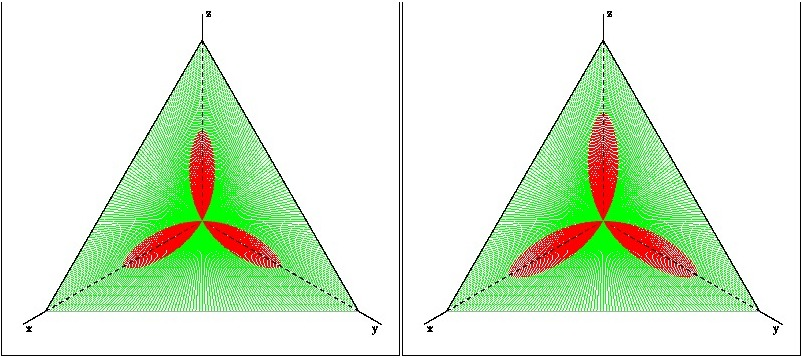
\includegraphics[width=\textwidth]{fleur-concat.png}
      \caption{\footnotesize These two diagrams illustrate
        inequalities (\ref{eq:iengaech}) and (\ref{eq:feovaivo}). The
        former displays all points in red which violate
        \textsc{collinear horizon}, measured from the centre. The
        latter displays points in different colours whose orientation
        of asymmetry differs, measured from the centre. The two red
        sets are not the same, but there appears to be a relationship,
        one that ultimately I suspect to be due to the more basic
        property of asymmetry.}
      \label{fig:eeghoomo}
    \end{minipage}
\end{figure}

The bitter aftertaste that remains with \textsc{collinear horizon} is
that it is opaque what motivates information theory not only to put
probability distributions farther apart near the periphery, as I would
expect, but also near the centre. I lack the epistemic intuition
reflected in the behaviour. The next subsection on asymmetry deals
with this lack of epistemic intuition writ large.

\subsection{Transitivity of Asymmetry}
\label{subsec:Asymmetry}

Recall Joyce's two axioms Weak Convexity and Symmetry (see page
\pageref{quot:weakconv}). The geometry of reason (certainly in its
Euclidean form) mandates Weak Convexity because the bisector of an
isosceles triangle is always shorter than the isosceles sides. Weak
Convexity, on the one hand, also holds for information theory (see
appendix~\ref{app:wcs} for a proof). Symmetry, on the
other hand, fails for information theory. Fortunately, although I do not
pursue this any further here, information theory arrives at many of
Joyce's results even without the violated axiom.

Asymmetry presents a problem for the geometry of reason as well as for
information theory. For the geometry of reason, the problem is akin to
\textsc{continuity}. For information theory, the problem is the
non-trivial nature of the asymmetries it induces, which somehow need
to be reconnected to epistemic justification. I will consider this
problem in a moment, but first I will have a look at the problem for
the geometry of reason.

Extreme probabilities are special and create asymmetries in updating:
moving in direction from certainty to uncertainty is asymmetrical to
moving in direction from uncertainty to certainty. Geometry of
reason's metric topology, however, allows for no asymmetries.

\begin{quotex}
  \beispiel{Extreme Asymmetry}\label{ex:extreme} Consider two cases
  where for case 1 the prior probabilities are $Y_{1}=(0.4,0.3,0.3)$
  and the posterior probabilities are $Y_{1}'=(0,0.5,0.5)$; for case 2
  the prior probabilities are reversed, so $Y_{2}=(0,0.5,0.5)$ and the
  posterior probabilities $Y_{2}'=(0.4,0.3,0.3)$.
\end{quotex}

{\noindent}Case 1 is a straightforward application of standard conditioning. Case
2 is more complicated: what does it take to raise a prior probability
of zero to a positive number? In terms of information theory, the
information required is infinite. Case 2 is also not compatible with
standard conditioning (at least not with what Alan H{\'a}jek calls the
ratio analysis of conditional probability, see \scite{7}{hajek03}{}).
The geometry of reason may want to solve this problem by signing on to
a version of regularity, but then it violates \textsc{regularity}.
Happy kids, clean house, sanity: the hapless homemaker must pick two.
The third remains elusive. Continuity, a consistent view of
regularity, and symmetry: the hapless geometer of reason cannot have
it all.

Now turn to the woes of the information theorist. Given the asymmetric
similarity measure of probability distributions that information
theory requires (the Kullback-Leibler divergence), a prior probability
distribution $P$ may be closer to a posterior probability distribution
$Q$ than $Q$ is to $P$ if their roles (prior-posterior) are reversed.
That is just what we would expect. The problem is that there is
another posterior probability distribution $R$ where the situation is
just the opposite: prior $P$ is further away from posterior $R$ than
prior $R$ is from posterior $P$. And whether a probability
distribution different from $P$ is of the $Q$-type or of the $R$-type
escapes any epistemic intuition.

For simplicity, let us consider probability distributions and their
associated credence functions on an event space with three atoms
$\Omega=\{\omega_{1},\omega_{2},\omega_{3}\}$. The simplex
$\mathbb{S}^{2}$ represents all of these probability distributions.
Every point $p$ in $\mathbb{S}^{2}$ representing a probability
distribution $P$ induces a partition on $\mathbb{S}^{2}$ into points
that are symmetric to $p$, positively skew-symmetric to $p$, and
negatively skew-symmetric to $p$ given the topology of information
theory.

In other words, if

\begin{equation}
  \label{eq:sksy}
  \Delta_{P}(P')=D_{\mbox{\tiny KL}}(P',P)-D_{\mbox{\tiny KL}}(P,P'),
\end{equation}

{\noindent}then, holding $P$ fixed, $\mathbb{S}^{2}$ is partitioned into three
regions, 

\begin{equation}
  \label{eq:sieruxis}
  \Delta^{-1}(\mathbb{R}_{>0})\hspace{.5in}\Delta^{-1}(\mathbb{R}_{<0})\hspace{.5in}\Delta^{-1}(\{0\})
\end{equation}

One could have a simple epistemic intuition such as \qnull{it takes
  less to update from a more uncertain probability distribution to a
  more certain probability distribution than the reverse direction,}
where the degree of certainty in a probability distribution is
measured by its entropy. This simple intuition accords with what we
said about extreme probabilities and it holds true for the asymmetric
distance measure defined by the Kullback-Leibler divergence in the
two-dimensional case where $\Omega$ has only two elements (see
appendix~\ref{app:asytwodims}).

In higher-dimensional cases, however, the tripartite partition
(\ref{eq:sieruxis}) is non-trivial---some probability distributions
are of the $Q$-type, some are of the $R$-type, and it is difficult to
think of an epistemic distinction between them that does not already
presuppose information theory. See {\igure}~\ref{fig:concat} for
graphical illustration of this point.

On any account of well-behaved and ill-behaved asymmetries, the
Kullback-Leibler divergence is ill-behaved. Of the four axioms as
listed by Ralph Kopperman for a distance measure $d$ (see
\scite{8}{kopperman88}{89}), the Kullback-Leibler divergence violates
both symmetry and triangularity, making it a \qnull{semi-quasimetric}:

\begin{enumerate}[(m1)]
\item $d(x,x)=0$
\item $d(x,z)\leq{}d(x,y)+d(y,z)$ (triangularity)
\item $d(x,y)=d(y,x)$ (symmetry)
\item $d(x,y)=0$ implies $x=y$ (separation)
\end{enumerate}

The Kullback-Leibler divergence not only violates symmetry and
triangularity, but also \textsc{transitivity of asymmetry}. For a
description of \textsc{transitivity of asymmetry} see List Two on page
\pageref{page:listtwo}. For an example of it, consider

\begin{equation}
  \label{eq:transviol}
    P_{1}=\left(\frac{1}{2},\frac{1}{4},\frac{1}{4}\right)  \hspace{.5in}
    P_{2}=\left(\frac{1}{3},\frac{1}{3},\frac{1}{3}\right) \hspace{.5in}
    P_{3}=\left(\frac{2}{5},\frac{2}{5},\frac{1}{5}\right)
\end{equation}

{\noindent}In the terminology of \textsc{transitivity of asymmetry} in List Two,
$(P_{1},P_{2})$ is asymmetrically positive, and so is $(P_{2},P_{3})$.
The reasonable expectation is that $(P_{1},P_{3})$ is asymmetrically
positive by transitivity, but for the example in (\ref{eq:transviol})
it is asymmetrically negative.

How counterintuitive this is (epistemically and otherwise) is
demonstrated by the fact that in MDS (the multi-dimensional scaling of
distance relationships) almost all asymmetric distance relationships
under consideration are asymmetrically transitive in this sense, for
examples see international trade in \scite{7}{chino78}{}; journal
citation in \scite{7}{coombs64}{}; car switch in
\scite{7}{harshmanetal82}{}; telephone calls in
\scite{7}{harshmanlundy84}{}; interaction or input-output flow in
migration, economic activity, and social mobility in
\scite{7}{coxonetal82}{}; flight time between two cities in
\scite{8}{gentleman06}{191}; mutual intelligibility between Swedish
and Danish in \scite{8}{vanommenetal13}{193}; Tobler's wind model in
\scite{7}{tobler75}{}; and the cyclist lovingly hand-sketched in
\scite{8}{kopperman88}{91}.

This \qnull{ill behaviour} of information theory begs for explanation,
or at least classification (it would help, for example, to know that
all reasonable non-commutative difference measures used for updating
are ill-behaved). Kopperman's objective is primarily to rescue
continuity, uniform continuity, Cauchy sequences, and limits for
topologies induced by difference measures which violate triangularity,
symmetry, and/or separation. Kopperman does not touch axiom (m1),
while in the psychological literature (see especially
\scite{7}{tversky77}{}) self-similarity is an important topic. This is
why an initially promising approach to asymmetric modeling in Hilbert
spaces by Chino (see \scite{7}{chino78}{}; \scite{7}{chino90}{};
\scite{7}{chinoshiraiwa93}{}; and \scite{7}{saburichino08}{}) will not
help us to distinguish well-behaved and ill-behaved asymmetries
between probability distributions. I am explaining the reasons in
appendix~\ref{app:eekiquom}.

The failure of Chino's modeling approach to make useful distinctions
among asymmetric distance measures between probability distributions
leads us to the more complex theory of information geometry and
differentiable manifolds. Both the results of Shun-ichi Amari (see
\scite{7}{amari85}{}; and \scite{7}{amarinagaoka00}{}) and Nikolai
Chentsov (see \scite{7}{chentsov82}{}) serve to highlight the special
properties of the Kullback-Leibler divergence, not without elevating
the discussion to a level of mathematical sophistication, however,
where it is difficult to retain the appeal to epistemic intuitions.
Information geometry considers probability distributions as
differentiable manifolds equipped with a Riemannian metric. This
metric, however, is Fisher's information metric, not the
Kullback-Leibler divergence, and it is defined on the tangent space of
the simplex representing finite-dimensional probability distributions.
There is a sense in which the Fisher information metric is the
derivative of the Kullback-Leibler divergence, and so the connection
to epistemic intuitions can be re-established.

For a future research project, it would be lovely either to see
information theory debunked in favour of an alternative geometry (this
chapter has demonstrated that this alternative will not be the geometry
of reason); or to see uniqueness results for the Kullback-Leibler
divergence to show that despite its ill behaviour the Kullback-Leibler
is the right asymmetric distance measure on which to base inference
and updating. Chentsov's theory of monotone invariance and Amari's
theory of $\alpha$-connections are potential candidates to provide
such results as well as an epistemic justification for information
theory.

Leitgeb and Pettigrew's reasoning to establish LP conditioning on the
basis of the geometry of reason is valid. Given the failure of LP
conditioning with respect to expectations in List One, it cannot be
sound. The premise to reject is the geometry of reason. A competing
approach, information theory, yields results that fulfill all of these
expectations except \textsc{horizon}. Information theory, however,
fails two other expectations identified in List Two---expectations
which the geometry of reason fulfills. We are left with loose ends and
ample opportunity for further work. The epistemic utility approach,
itself a relatively recent phenomenon, needs to come to a deeper
understanding of its relationship with information theory. It is an
open question, for example, if it is possible to provide a complete
axiomatization consistent with information theory to justify
probabilism, standard conditioning, and Jeffrey conditioning from an
epistemic utility approach as Shore and Johnston have done from a
pragmatic utility approach. It is also an open question, given the
results of this chapter, if there is hope reconciling information theory
with intuitions we have about epistemic utility and its attendant
quantitative concept of difference for partial beliefs.

\chapter{A Natural Generalization of Jeffrey Conditioning}
\label{chp:eejiegei}

\section{Two Generalizations}
\label{sec:euboonei}

Standard conditioning in Bayesian probability theory gives us a
relatively well-accepted tool to update on the observation of an
event. Jeffrey conditioning provides another tool which updates
probability distributions (or densities, from now on omitted) given
uncertain evidence. Jeffrey conditioning generalizes standard
conditioning. Evidence can be viewed as imposing a constraint on
acceptable probability distributions, often one with which the prior
probability distribution is inconsistent. If it is a conditional which
constitutes this constraint, standard conditioning and Jeffrey
conditioning do not always apply. Carl Wagner presents such a case
(see \scite{7}{wagner92}{}) together with a solution based on a
plausible intuition. We will call this intuition (W). Wagner's (W)
solution, or Wagner conditioning, in its turn generalizes Jeffrey
conditioning.

Twenty years earlier, E.T. Jaynes had already proposed a
generalization of Jeffrey conditioning, the principle of maximum
entropy \textsc{pme}. This generalization is more sweeping than
Wagner's and includes partial information cases (using the moment(s)
of a distribution as evidence), such as Bas van Fraassen's \emph{Judy
  Benjamin} problem and Jaynes' own \emph{Brandeis Dice} problem (see
{\xample}~\ref{ex:brandeis}). This chapter is concerned with a Wagner
type generalization of Jeffrey conditioning. For partial information
cases see chapter \ref{chp:eeyijeen}. Figure \ref{fig:aff} shows a
diagram of how these cases generalize.

Wagner investigates whether his generalization (W) agrees with
\textsc{pme}, finding that it does not. He then uses his method not
only to present a \qeins{natural generalization of Jeffrey
  conditioning} (see \scite{8}{wagner92}{250}), but also to deepen
criticism of \textsc{pme}. I will show that \textsc{pme} not only
generalizes Jeffrey conditioning (as is well known, for a formal proof
see \scite{7}{catichagiffin06}{}) but also Wagner conditioning.
Wagner's intuition (W) is plausible, and his method works. His
derivation of a disagreement with \textsc{pme}, however, is
conceptually more complex than he assumes. 

Below, we will show that \textsc{pme} and (W) are consistent given
(L). (L) is what I call the Laplacean principle which requires a
rational agent, besides other standard Bayesian commitments, to hold
sharp credences with respect to well-defined events under
consideration. (I), which is inconsistent with (L) and which some
Bayesians accept, allows a rational agent to have indeterminate or
imprecise credences (see \scite{7}{ellsberg61}{}; \scite{7}{levi85}{};
\scite{7}{walley91}{}; and \scite{7}{joyce10i}{}).

\medskip

\begin{tabular}{|c|c|c|c|c|l|}\hline
\textsc{pme} & (W) & (I) & (L) & & \\ \hline
$\bullet$ & $\bullet$ &  & & $\times$ & according to Wagner's article \\ \hline
$\bullet$ & $\bullet$ &  & & \checkmark & according to this article \\ \hline
& & $\bullet$ & $\bullet$ & $\times$ & disagree over permitting mushy credences \\ \hline
$\bullet$ & $\bullet$ & $\bullet$ & & $\times$ & formally shown in Wagner's article \\ \hline
$\bullet$ & $\bullet$ & & $\bullet$ & \checkmark & formally shown in this article \\ \hline 
\end{tabular}

\medskip

While Wagner is welcome to deny (L), my sense is that advocates of \textsc{pme}
usually accept it because they are already to the moderate right of
Sandy L. Zabell's spectrum between left-wing dadaists and right-wing
totalitarians (see \scite{8}{zabell05}{27}; Zabell's representative of
right-wing totalitarianism is E.T. Jaynes). If there were an advocate
of \textsc{pme} sympathetic to (I), Wagner's result would indeed force her to
choose. Wagner's criticism of \textsc{pme} is misplaced, however, since it
rests on a hidden assumption that someone who believes in \textsc{pme} would
tend not to hold. Wagner does not give an independent argument for
(I). This chapter shows how elegantly \textsc{pme} generalizes not only standard
conditioning and Jeffrey conditioning but also Wagner conditioning,
once we accept (L). In chapter \ref{chp:eingeili}, I provide
independent reasons why we should accept (L).

A tempered and differentiated account of \textsc{pme} (contrasted with
Jaynes' right-wing earlier version) is not only largely immune to
criticisms, but often illuminates the problems that the criticisms
pose (for example in the \emph{Judy Benjamin} case, see chapter
\ref{chp:eeyijeen}). This account rests on principles such as (L) and
a reasonable interpretation of what we mean by objectivity. To make
this more clear, and before we launch into the formalities of
generalizing Wagner conditioning by using \textsc{pme}, let us
articulate (L) and \textsc{pme}. (L) is what I call the Laplacean
principle and in addition to standard Bayesian commitments states that
a rational agent assigns a determinate precise probability to a
well-defined event under consideration (for a defence of (L) against
(I) see \scite{7}{white10}{}; and \scite{7}{elga10}{}).

To avoid excessive apriorism (see \scite{7}{seidenfeld79}{414}), (L)
does not require that a rational agent has probabilities assigned to
all events in an event space, only that, once an event has been
brought to attention, and sometimes retrospectively, the rational
agent is able to assign a sharp probability (for more detail on this
issue and some rules which propositions need to be assigned subjective
probabilities see \scite{8}{hajek03}{313}). Newton did not need to
have a prior probability for Einstein's theory in order to have a
posterior probability for his theory of gravity.

(L) also does not require objectivity in the sense that all rational
agents must agree in their probability distributions if they have the
same information. It is important to distinguish between type I and
type II prior probabilities (I have also been calling them absolutely
and relatively prior probabilities). The former precede any
information at all (so-called ignorance priors). The latter are simply
prior relative to posterior probabilities in probability kinematics.
They may themselves be posterior probabilities with respect to an
earlier instance of probability kinematics.

The case for objectivity in probability kinematics, where prior
probabilities are of type II, is consistent with and dependent on a
subjectivist interpretation of probabilities, making for some
terminological confusion. Interpretations of the evidence and how it
is to be cast in terms of formal constraints may vary. Once we agree
on a prior distribution (type II), however, and on a set of formal
constraints representing our evidence, \textsc{pme} claims that
posterior probabilities follow mechanically. Just as is the case in
deductive logic, we may come to a tentative and voluntary agreement on
an interpretation, a set of rules and presuppositions and then go part
of the way together. For the interplay between \textsc{pme} and
\emph{Infomin}, see section~\ref{sec:oxiequei}.

Some advocates of \textsc{pme} may find (L) too weak in its claims,
but none think it is too strong. Once (L) is assumed, however,
Wagner's diagnosis of disagreement between (W) and \textsc{pme} fails.
Moreover, \textsc{pme} and (L) together seamlessly generalize Wagner
conditioning. In the remainder of this chapter~I will provide a sketch
of a formal proof for this claim. A welcome side-effect of reinstating
harmony between \textsc{pme} and (W) is that it provides an inverse
procedure to Vladim{\'\i}r Majern{\'\i}k's method of finding marginals
based on given conditional probabilities (see \scite{7}{majernik00}{};
and section \ref{sec:uodeigei}).

\section{Wagner's Natural Generalization of Jeffrey Conditioning}
\label{sec:feeriesh}

Wagner claims that he has found a relatively common case of
probability kinematics in which \textsc{pme} delivers the wrong result
so that we must develop an ad hoc generalization of Jeffrey
conditioning. This is best explained by using Wagner's example, the
\emph{Linguist} problem (see \scite{8}{wagner92}{252} and
\scite{8}{spohn12}{197}).

\begin{quotex}
  \beispiel{Linguist}\label{ex:linguist} You encounter the native of a
  certain foreign country and wonder whether he is a Catholic
  northerner ($\theta_{1}$), a Catholic southerner ($\theta_{2}$), a
  Protestant northerner ($\theta_{3}$), or a Protestant southerner
  ($\theta_{4}$). Your prior probability $p$ over these possibilities
  (based, say, on population statistics and the judgment that it is
  reasonable to regard this individual as a random representative of
  his country) is given by
  $p(\theta_{1})=0.2,p(\theta_{2})=0.3,p(\theta_{3})=0.4,\mbox{ and
  }p(\theta_{4})=0.1$.
  The individual now utters a phrase in his native tongue which, due
  to the aural similarity of the phrases in question, might be a
  traditional Catholic piety ($\omega_{1}$), an epithet
  uncomplimentary to Protestants ($\omega_{2}$), an innocuous southern
  regionalism ($\omega_{3}$), or a slang expression used throughout
  the country in question ($\omega_{4}$). After reflecting on the
  matter you assign subjective probabilities
  $u(\omega_{1})=0.4,u(\omega_{2})=0.3,u(\omega_{3})=0.2,\mbox{ and
  }u(\omega_{4})=0.1$
  to these alternatives. In the light of this new evidence how should
  you revise $p$?
\end{quotex}

Let
$\Theta=\{\theta_{i}:i=1,\ldots,4\},\Omega=\{\omega_{i}:i=1,\ldots,4\}$.
Let $\Gamma:\Omega\rightarrow{}2^{\Theta}-\{\emptyset\}$ be the
function which maps $\omega$ to $\Gamma(\omega)$, the narrowest event
in $\Theta$ entailed by the outcome $\omega\in\Omega$. Here are two
definitions that take advantage of the apparatus established by Arthur
Dempster (see \scite{7}{dempster67}{}). We will need $m$ and $b$ to
articulate Wagner's (W) solution for \emph{Linguist} type problems.

\begin{equation}
  \mbox{For all }E\subseteq{}\Theta, m(E)=u(\{\omega\in\Omega:\Gamma(\omega)=E\})\label{eq:mof}.
\end{equation}

\begin{equation}
  \mbox{For all }E\subseteq{}\Theta, b(E)=\sum_{H\subseteq{}E}m(H)=u(\{\omega\in\Omega:\Gamma(\omega)\subseteq{}E\})\label{eq:bof}.
\end{equation}

Let $Q$ be the posterior joint probability measure on
$\Theta\times\Omega$, and $Q_{\Theta}$ the marginalization of $Q$ to
$\Theta$, $Q_{\Omega}$ the marginalization of $Q$ to $\Omega$.
Wagner plausibly suggests that $Q$ is compatible with $u$ and $\Gamma$
if and only if

\begin{equation}
  \label{eq:entail}
  \mbox{for all }\theta\in\Theta\mbox{ and for all
  }\omega\in\Omega,\theta\notin\Gamma(\omega)\mbox{ implies that }Q(\theta,\omega)=0
\end{equation}

{\noindent}and

\begin{equation}
  \label{eq:marg}
  Q_{\Omega}=u.
\end{equation}

The two conditions (\ref{eq:entail}) and (\ref{eq:marg}), however, are
not sufficient to identify a \qeins{uniquely acceptable revision of a
  prior} \scite{2}{wagner92}{250}. Wagner's proposal includes a third
condition, which extends Jeffrey's rule to the situation at hand. We
will call it (W). To articulate the condition, we need some more
definitions. For all $E\subseteq{}\Theta$, let
$E_{\bigstar}=\{\omega\in\Omega:\Gamma(\omega)=E\}$, so that
$m(E)=u(E_{\bigstar})$. For all $A\subseteq\Theta$ and all
$B\subseteq\Omega$, let $\mbox{``A''}=A\times\Omega$ and
$\mbox{``B''}=\Theta\times{}B$, so that
$Q(\mbox{``A''})=Q_{\Theta}(A)$ for all $A\subseteq\Theta$ and
$Q(\mbox{``B''})=Q_{\Omega}(B)$ for all $B\subseteq\Omega$. Let also
$\mathcal{E}=\{E\subseteq\Theta:m(E)>0\}$ be the family of evidentiary
focal elements.

According to Wagner only those $Q$ satisfying the condition

\begin{equation}
  \label{eq:wagn}
  \mbox{for all }A\subseteq\Theta\mbox{ and for all }E\in\mathcal{E},Q(\mbox{``A''}|\mbox{``E$_{\bigstar}$''})=p(A|E)
\end{equation}

are eligible candidates for updated joint probabilities in
\emph{Linguist} type problems. 
To adopt (\ref{eq:wagn}), says Wagner, is to make sure
that the total impact of the occurrence of the event $E_{\bigstar}$ is
to preclude the occurrence of any outcome $\theta\notin{}E$, and that,
within $E$, $p$ remains operative in the assessment of relative
uncertainties (see \scite{8}{wagner92}{250}). While conditions
(\ref{eq:entail}), (\ref{eq:marg}) and (\ref{eq:wagn}) may admit an
infinite number of joint probability distributions on
$\Theta\times\Omega$, their marginalizations to $\Theta$ are identical
and give us the desired posterior probability, expressible by the
formula

\begin{equation}
  \label{eq:qofa}
  q(A)=\sum_{E\in\mathcal{E}}m(E)p(A|E).
\end{equation}

So far we are in agreement with Wagner. Wagner's scathing verdict
about \textsc{pme} towards the end of his article, however, is not really a
verdict about \textsc{pme} in the Laplacean tradition but about the curious
conjunction of \textsc{pme} and (I):

\begin{quotex}
  Students of maximum entropy approaches to probability revision may
  [\ldots] wonder if the probability measure defined by our formula
  (\ref{eq:qofa}) similarly minimizes [the Kullback-Leibler
  information number] $D_{\textsc{kl}}(q,p)$ over all probability
  measures $q$ bounded below by $b$. The answer is negative [\ldots]
  convinced by Skyrms, among others, that \textsc{pme} is not a
  tenable updating rule, we are undisturbed by this fact. Indeed, we
  take it as additional evidence against \textsc{pme} that
  (\ref{eq:qofa}), firmly grounded on [\ldots] a considered judgment
  that (\ref{eq:wagn}) holds, might violate \textsc{pme} [\ldots]
  the fact that Jeffrey's rule coincides with \textsc{pme} is
  simply a misleading fluke, put in its proper perspective by the
  natural generalization of Jeffrey conditioning described in
  this paper. [References to formulas and notation modified.]
  \scite{3}{wagner92}{255}
\end{quotex}

In the next section, we will contrast what Wagner considers to be the
solution of \textsc{pme} for this problem, \qnull{Wagner's \textsc{pme} solution,} and
Wagner's solution presented in this section, \qnull{Wagner's (W)
  solution,} and show, in much greater detail than Wagner does, why
Wagner's \textsc{pme} solution misrepresents \textsc{pme}.

\section{Wagner's PME Solution}
\label{sec:gaephuiw}

Wagner's \textsc{pme} solution assumes the constraint that $b$ must act as a
lower bound for the posterior probability. Consider
$E_{12}=\{\theta_{1}\vee\theta_{2}\}$. Because both $\omega_{1}$ and
$\omega_{2}$ entail $E_{12}$, according to (\ref{eq:bof}),
$b(E_{12})=0.70$. It makes sense to consider it a constraint that the
posterior probability for $E_{12}$ must be at least $b(E_{12})$. Then
we choose from all probability distributions fulfilling the constraint
the one which is closest to the prior probability distribution, using
the Kullback-Leibler divergence.

Wagner applies this idea to the marginal probability distribution on
$\Theta$. He does not provide the numbers, but refers to simpler
examples to make his point that \textsc{pme} does not generally agree with his
solution. To aid the discussion, I want to populate Wagner's claim for
the \emph{Linguist} problem with numbers. Using proposition 1.29 in
Dimitri Bertsekas' book \emph{Constrained Optimization and Lagrange
  Multiplier Methods} (see \scite{8}{bertsekas82}{71}) and some
non-trivial calculations, Wagner's \textsc{pme} solution for the
\emph{Linguist} problem (indexed $Q_{wm}$) is

\begin{equation}
  \label{eq:p13}
  \tilde{\beta}=(Q_{wm}(\theta_{j}))^{\intercal}=(0.30,0.45,0.10,0.15)^{\intercal}.
\end{equation}

{\noindent}A brief remark about notation: I will use $\alpha$ for vectors
expressing $\omega_{i}$ probabilities and $\beta$ for vectors
expressing $\theta_{j}$ probabilities. I will use a tilde as in
$\tilde{\beta}$ or a hat as in $\hat{\beta}$ for posteriors, while
priors remain without such ornamentation. The tilde is used for
Wagner's \textsc{pme} solution (which, as we will see, is incorrect) and the
hat for the correct solution (both (W) and \textsc{pme}).

The cross-entropy between $\tilde{\beta}$ and the prior

\begin{equation}
  \label{eq:p14}
  \beta=(P(\theta_{j}))^{\intercal}=(0.20,0.30,0.40,0.10)^{\intercal}
\end{equation}

{\noindent}is indeed significantly smaller than the cross-entropy between
Wagner's (W) solution 

\begin{equation}
  \label{eq:p15}
  \hat{\beta}=(Q(\theta_{j}))^{\intercal}=(0.30,0.60,0.04,0.06)^{\intercal}
\end{equation}

{\noindent}and the prior $\beta$ ($0.0823$ compared to $0.4148$). For the
cross-entropy, we use the Kullback-Leibler Divergence

\begin{equation}
  \label{eq:kl}
  D_{\textsc{kl}}(q,p)=\sum_{j}q(\theta_{j})\log_{2}\frac{q(\theta_{j})}{p(\theta_{j})}.
\end{equation}

From the perspective of an \textsc{pme} advocate, there are only two
explanations for this difference in cross-entropy. Either Wagner's (W)
solution illegitimately uses information not contained in the problem,
or Wagner's \textsc{pme} solution has failed to include information that is
contained in the problem. I will simplify the \emph{Linguist} problem
in order to show that the latter is the case.

\begin{quotex}
  \beispiel{Simplified Linguist}\label{ex:simpllinguist} Imagine the
  native is either Protestant or Catholic (50:50). Further imagine
  that the utterance of the native either entails that the native is a
  Protestant (60\%) or provides no information about the religious
  affiliation of the native (40\%).
\end{quotex}

Using (\ref{eq:qofa}), the posterior probability distribution is 80:20
(Wagner's (W) solution and, surely, the correct solution). Using $b$
as a lower bound and \textsc{pme}, Wagner's \textsc{pme} solution for this radically
simplified problem is 60:40, clearly a more entropic solution than
Wagner's (W) solution. The problem, as we will show, is that Wagner's
\textsc{pme} solution does not take into account (L), which an \textsc{pme} advocate
would naturally accept.

For a Laplacean, the prior joint probability distribution on
$\Theta\times\Omega$ is not left unspecified for the calculation of
the posteriors. Before the native makes the utterance, the event space
is unspecified with respect to $\Omega$. After the utterance, however,
the event space is defined (or brought to attention) and populated by
prior probabilities according to (L). That this happens
retrospectively may or may not be a problem: Bayes' theorem is
frequently used retrospectively, for example when the anomalous
precession of Mercury's perihelion, discovered in the mid-1800s, was
used to confirm Albert Einstein's General Theory of Relativity in 1915
(for retrospective conditioning see \scite{7}{grovehalpern97}{}; and
\scite{8}{diaconiszabell82}{822}). I shall bracket for now that this
procedure is controversial and refer the reader to the literature on
Old Evidence.

Ariel Caticha and Adom Giffin make the following
appeal:

\begin{quotex}
  Bayes' theorem requires that $P(\omega,\theta)$ be defined and that
  assertions such as \qzwei{$\omega$ \emph{and} $\theta$} be
  meaningful; the relevant space is neither $\Omega$ nor $\Theta$ but
  the product $\Omega\times\Theta$ [notation modified]
  \scite{3}{catichagiffin06}{9}
\end{quotex}

Following (L) we shall populate the joint probability matrix $P$ on
$\Omega\times\Theta$, which is a perfect task for \textsc{pme}, as
updating the joint probability $P$ to $Q$ on $\Omega\times\Theta$ will
be a perfect task for \emph{Infomin}. For the \emph{Simplified
  Linguist} problem, this procedure gives us the correct result,
agreeing with Wagner's (W) solution (80:20).

There is a more general theorem which incorporates Wagner's (W) method
into Laplacean realism and \textsc{pme} orthodoxy. The proof of this
theorem is in the next section. Its validity is confirmed by how well
it works for the \emph{Linguist} problem (as well as the
\emph{Simplified Linguist} problem).

We have not yet formally demonstrated that for all Wagner-type
problems $(\beta,\hat{\alpha},\kappa)$, the correct \textsc{pme}
solution (versus Wagner's deficient \textsc{pme} solution) agrees with
Wagner's (W) solution, although we have established a useful framework
and demonstrated the agreement for the \emph{Linguist} problem. As
Vladim{\'\i}r Majern{\'\i}k has shown how to derive marginal
probabilities from conditional probabilities using \textsc{pme} (see
\scite{7}{majernik00}{}), in the next section I will inversely show
how to derive conditional probabilities (i.e.\ the joint probability
matrices) from the marginal probabilities and logical relationships
provided in Wagner-type problems. This technical result together with
the claim established in the present paper that Wagner's intuition (W)
is consistent with \textsc{pme}, given (L), underlines the formal and
conceptual virtue of \textsc{pme}.

\section{Maximum Entropy and Probability Kinematics Constrained by Conditionals}
\label{sec:uodeigei}

Jeffrey conditioning is a method of update (recommended first by
Richard Jeffrey in \scite{7}{jeffrey65}{}) which generalizes standard
conditioning and operates in probability kinematics where evidence is
uncertain ($P(E)\neq{}1$). Sometimes, when we reason inductively,
outcomes that are observed have entailment relationships with
partitions of the possibility space that pose challenges that Jeffrey
conditioning cannot meet. As we will see, it is not difficult to
resolve these challenges by generalizing Jeffrey conditioning. There
are claims in the literature that the principle of maximum entropy,
from now on \textsc{pme}, conflicts with this generalization. I will
show under which conditions this conflict obtains. Since proponents of
\textsc{pme} are unlikely to subscribe to these conditions, the
position of \textsc{pme} in the larger debate over inductive logic and
reasoning is not undermined.

In his paper \qeins{Marginal Probability Distribution Determined by
  the Maximum Entropy Method} (see \scite{7}{majernik00}{}),
Vladim{\'\i}r Majern{\'\i}k asks the following question: If we had two
partitions of an event space and knew all the conditional
probabilities (any conditional probability of one event in the first
partition conditional on another event in the second partition), would
we be able to calculate the marginal probabilities for the two
partitions? The answer is yes, if we commit ourselves to \textsc{pme}.

For Majern{\'\i}k's question, \textsc{pme} provides us with a unique
and plausible answer. We may also be interested in the obverse
question: if the marginal probabilities of the two partitions were
given, would we similarly be able to calculate the conditional
probabilities? The answer is yes: given \textsc{pme}, Theorems 2.2.1.
and 2.6.5. in \scite{7}{coverthomas06}{} reveal that the joint
probabilities are the product of the marginal probabilities (see also
\scite{7}{debbahmueller05}{}). Once the joint probabilities and the
marginal probabilities are available, it is trivial to calculate the
conditional probabilities.

It is important to note that these joint probabilities do not
legislate independence, even though they allow it. M{\'e}rouane Debbah
and Ralf M{\"u}ller correctly describe these joint probabilities as a
model with as many degrees of freedom as possible, which leaves free
degrees for correlation to exist or not (see
\scite{8}{debbahmueller05}{1674}). This avoids the introduction of
unjustified information corresponding to the simple intuition behind
\textsc{pme}: when updating your probabilities, waste no useful
information and do not gain information unless the evidence compels
you to gain it (see \scite{8}{fraassenetal86}{376};
\scite{7}{zellner88}{}; \scite{7}{jaynes88}{}; and
\scite{8}{palmiericiuonzo13}{186}). The principle comes with its own
formal apparatus, not unlike probability theory itself: Shannon's
information entropy (see \scite{7}{shannon48}{}), the Kullback-Leibler
divergence (see \scite{7}{kullbackleibler51}{};
\scite{7}{kullback59}{}; \scite{8}{guiasu77}{308ff}; and
\scite{8}{seidenfeld86}{262ff}), the use of Lagrange multipliers (see
\scite{8}{coverthomas06}{409ff}; \scite{8}{guiasu77}{327f}; and
\scite{8}{seidenfeld86}{281}), and the log-inverse relationship
between information and probability (see \scite{7}{kampe67}{};
\scite{7}{ingardenurbanik62}{}; \scite{7}{khinchin57}{}; and
\scite{7}{kolmogorov68}{}). 

The \emph{Linguist} problem by Carl Wagner can be cast in similar
terms as Majern{\'\i}k's. If we were given some of the marginal
probabilities in an updating problem as well as some logical
relationships between the two partitions, would we be able to
calculate the remaining marginal probabilities? This problem is best
understood by example (see Wagner's \emph{Linguist} problem in
section~\ref{sec:feeriesh}). Wagner solves it using a natural
generalization of Jeffrey conditioning, which I will call Wagner
conditioning. It is not based on \textsc{pme}, but on what I call
Jeffrey's updating principle, or \textsc{jup} for short:

\begin{quotex}
  [\textsc{jup}] In a diachronic updating process, keep the ratio of
  probabilities constant as long as they are unaffected by the
  constraints that the evidence poses.
\end{quotex}

{\noindent}\textsc{jup} is at the heart of principle (L) in the previous
sections. This section resists Wagner's conclusions and shows in more
technical detail than previously that \textsc{pme} generalizes both
Jeffrey conditioning and Wagner conditioning, providing a much more
integrated approach to probability updating. This integrated approach
also gives a coherent answer to the obverse Majern{\'\i}k problem
posed above.

Richard Jeffrey proposes an updating method for cases in which the
evidence is uncertain, generalizing standard probabilistic
conditioning. I will present this method in unusual notation,
anticipating using my notation to solve Wagner's \emph{Linguist}
problem and to give a general solution for the obverse Majern{\'\i}k
problem. Let $\Omega$ be a finite event space and
$\{\theta_{j}\}_{j=1,\ldots,n}$ a partition of $\Omega$. Let $\kappa$
be an $m\times{}n$ matrix for which each column contains exactly one
$1$, otherwise $0$. Let $P=P_{\mbox{\tiny{prior}}}$ and
$\hat{P}=P_{\mbox{\tiny{posterior}}}$. Then
$\{\omega_{i}\}_{i=1,\ldots,m}$, for which

\begin{equation}
  \label{eq:m1}
  \omega_{i}=\bigcup_{j=1,\dots,n}\theta^{*}_{ij},
\end{equation}

{\noindent}is likewise a partition of $\Omega$ (the $\omega$ are
basically a more coarsely grained partition than the $\theta$).
$\theta^{*}_{ij}=\emptyset$ if $\kappa_{ij}=0$,
$\theta^{*}_{ij}=\theta_{j}$ otherwise. Let $\beta$ be the vector of
prior probabilities for $\{\theta_{j}\}_{j=1,\ldots,n}
(P(\theta_{j})=\beta_{j})$ and $\hat{\beta}$ the vector of posterior
probabilities $(\hat{P}(\theta_{j})=\hat{\beta}_{j})$; likewise for
$\alpha$ and $\hat{\alpha}$ corresponding to the prior and posterior
probabilities for $\{\omega_{i}\}_{i=1,\ldots,m}$, respectively.

A Jeffrey-type problem is when $\beta$ and $\hat{\alpha}$ are given
and we are looking for $\hat{\beta}$. A mathematically more concise
characterization of a Jeffrey-type problem is the triple
$(\kappa,\beta,\hat{\alpha})$. The solution, using Jeffrey
conditioning, is

\begin{equation}
  \label{eq:m2}
  \hat{\beta_{j}}=\beta_{j}\sum_{i=1}^{n}\frac{\kappa_{ij}\hat{\alpha_{i}}}{\sum_{l=1}^{m}\kappa_{il}\beta_{l}}\mbox{ for all }j=1,\ldots,n.
\end{equation}

{\noindent}The notation is more complicated than it needs to be for Jeffrey
conditioning. In section~\ref{chp:eejiegei}, however, I will take
full advantage of it to present a generalization where the
$\omega_{i}$ do not range over the $\theta_{j}$. In the meantime, here
is an example to illustrate (\ref{eq:m2}).

\begin{quotex}
  \beispiel{Colour Blind}\label{ex:colblind} A token is pulled from a
  bag containing 3 yellow tokens, 2 blue tokens, and 1 purple token.
  You are colour blind and cannot distinguish between the blue and the
  purple token when you see it. When the token is pulled, it is shown
  to you in poor lighting and then obscured again. 
\end{quotex}

{\noindent}You come to the conclusion based on your observation that
the probability that the pulled token is yellow is $1/3$ and that the
probability that the pulled token is blue or purple is $2/3$. What is
your updated probability that the pulled token is blue? Let
$P(\mbox{blue})$ be the prior subjective probability that the pulled
token is blue and $\hat{P}(\mbox{blue})$ the respective posterior
subjective probability. Jeffrey conditioning, based on \textsc{jup}
(which mandates, for example, that
$\hat{P}(\mbox{blue}|\mbox{blue or}\mbox{
  purple})=P(\mbox{blue}|\mbox{blue or purple})$) recommends

\begin{align}
  \label{eq:jcs}
&\hat{P}(\mbox{blue})&=&\hat{P}(\mbox{blue}|\mbox{blue or purple})\hat{P}(\mbox{blue or
  purple})+\notag \\
&&&\hat{P}(\mbox{blue}|\mbox{neither blue nor
  purple})\hat{P}(\mbox{neither blue nor purple})\notag \\
&&=&P(\mbox{blue}|\mbox{blue or purple})\hat{P}(\mbox{blue or
  purple})=4/9
\end{align}

{\noindent}In the notation of (\ref{eq:m2}), {\xample}
\ref{ex:colblind} is calculated with
$\beta=(1/2,1/3,1/6)^{\top},\hat{\alpha}=(1/3,2/3)^{\top}$,

\begin{equation}
  \label{eq:kappa}
  \kappa=\left[
  \begin{array}{ccc}
    1 & 0 & 0 \\
    0 & 1 & 1
  \end{array}\right]
\end{equation}

{\noindent}and yields the same result as (\ref{eq:jcs}) with
$\hat{\beta}_{2}=4/9$.

Wagner's \emph{Linguist} problem is an instance of the more general
obverse Majern{\'\i}k problem where partitions are given with logical
relationships between them as well as some marginal probabilities.
Wagner-type problems seek as a solution missing marginals, while
obverse Majern{\'\i}k problems seek the conditional probabilities as
well, both of which I will eventually provide using \textsc{pme}.

Wagner's solution for such problems (from now on Wagner conditioning)
rests on \textsc{jup} and a formal apparatus established by Arthur
Dempster (see \scite{7}{dempster67}{}), which is quite different from
our notational approach. One advantage of \textsc{pme} is that it
works on the wide domain of updating problems where the evidence
corresponds to an affine constraint (for affine constraints see
\scite{7}{csiszar67}{}; for problems with evidence not in the form of
affine constraints see \scite{7}{paris06}{}). Updating problems where
standard conditioning and Jeffrey conditioning are applicable are a
subset of this domain (see figure~\ref{fig:aff}). Wagner's contention
is that on the wider domain of problems where we must use Wagner
conditioning (and which he does not cast in terms of affine
constraints), \textsc{jup} and \textsc{pme} contradict each other. We
are now in the awkward position of being confronted with two plausible
intuitions, \textsc{jup} and \textsc{pme}, and it appears that we have
to let one of them go.

In order to show how \textsc{pme} generalizes Jeffrey conditioning
(see subsection~\ref{subsec:ukotooje}) and Wagner conditioning to
boot, I use the notation that I have already introduced for Jeffrey
conditioning. We can characterize Wagner-type problems analogously to
Jeffrey-type problems by a triple $(\kappa,\beta,\hat{\alpha})$.
$\{\theta_{j}\}_{j=1,\ldots,n}$ and $\{\omega_{i}\}_{i=1,\ldots,m}$
now refer to independent partitions of $\Omega$, i.e.\ (\ref{eq:m1})
need not be true. Besides the marginal probabilities
$P(\theta_{j})=\beta_{j}, \hat{P}(\theta_{j})=\hat{\beta}_{j},
P(\omega_{i})=\alpha_{i},\hat{P}(\omega_{i})=\hat{\alpha}_{i}$,
we therefore also have joint probabilities
$\mu_{ij}=P(\omega_{i}\cap\theta_{j})$ and
$\hat{\mu}_{ij}=\hat{P}(\omega_{i}\cap\theta_{j})$.

Given the specific nature of Wagner-type problems, there are a few
constraints on the triple $(\kappa,\beta,\hat{\alpha})$. The last row
$(\mu_{mj})_{j=1,\ldots,n}$ is special because it represents the
probability of $\omega_{m}$, which is the negation of the events
deemed possible after the observation. In the \emph{Linguist} problem,
for example, $\omega_{5}$ is the event (initially highly likely, but
impossible after the observation of the native's utterance) that the
native does not make any of the four utterances. The native may have,
after all, uttered a typical Buddhist phrase, asked where the nearest
bathroom was, complimented your fedora, or chosen to be silent.
$\kappa$ will have all $1$s in the last row. Let
$\hat{\kappa}_{ij}=\kappa_{ij}$ for $i=1,\ldots,m-1$ and
$j=1,\ldots,n$; and $\hat{\kappa}_{mj}=0$ for $j=1,\ldots,n$.
$\hat{\kappa}$ equals $\kappa$ except that its last row are all $0$s,
and $\hat{\alpha}_{m}=0$. Otherwise the $0$s are distributed over
$\kappa$ (and equally over $\hat{\kappa}$) so that no row and no
column has all $0$s, representing the logical relationships between
the $\omega_{i}$s and the $\theta_{j}$s ($\kappa_{ij}=0$ if and only
if $\hat{P}(\omega_{i}\cap\theta_{j})=\mu_{ij}=0$). We set
$P(\omega_{m})=x$ ($\hat{P}(\omega_{m})=0$), where $x$ depends on the
specific prior knowledge. Fortunately, the value of $x$ cancels out
nicely and will play no further role. For convenience, we define

\begin{equation}
\label{eq:zeta}
\zeta=(0,\ldots,0,1)^{\top}
\end{equation}

{\noindent}with $\zeta_{m}=1$ and $\zeta_{i}=0$ for $i\neq{}m$.

The best way to visualize such a problem is by providing the joint
probability matrix $M=(\mu_{ij})$ together with the marginals $\alpha$
and $\beta$ in the last column/row, here for example as for the
\emph{Linguist} problem with $m=5$ and $n=4$ (note that this is not
the matrix $M$, which is $m\times{}n$, but $M$ expanded with the
marginals in improper matrix notation):

\begin{equation}
  \label{eq:m3}
      \left[
      \begin{array}{ccccc}
        \mu_{11} & \mu_{12} & 0 & 0 & \alpha_{1} \\
        \mu_{21} & \mu_{22} & 0 & 0 & \alpha_{2} \\
        0 & \mu_{32} & 0 & \mu_{34} & \alpha_{3} \\
        \mu_{41} & \mu_{42} & \mu_{43} & \mu_{44} & \alpha_{4} \\
        \mu_{51} & \mu_{52} & \mu_{53} & \mu_{54} & x \\
        \beta_{1} & \beta_{2} & \beta_{3} & \beta_{4} & 1.00
      \end{array}
\right].
\end{equation}

{\noindent}The $\mu_{ij}\neq{}0$ where $\kappa_{ij}=1$. Ditto, mutatis mutandis,
for $\hat{M},\hat{\alpha},\hat{\beta}$. To make this a little less
abstract, Wagner's \emph{Linguist} problem is characterized by the
triple $(\kappa,\beta,\hat{\alpha})$,

\begin{equation}
  \label{eq:m4}
  \kappa=\left[
  \begin{array}{cccc}
    1 & 1 & 0 & 0 \\
    1 & 1 & 0 & 0 \\
    0 & 1 & 0 & 1 \\
    1 & 1 & 1 & 1 \\
    1 & 1 & 1 & 1
  \end{array}
\right]\mbox{ and }
  \hat{\kappa}=\left[
  \begin{array}{cccc}
    1 & 1 & 0 & 0 \\
    1 & 1 & 0 & 0 \\
    0 & 1 & 0 & 1 \\
    1 & 1 & 1 & 1 \\
    0 & 0 & 0 & 0
  \end{array}
\right]
\end{equation}

\begin{equation}
  \label{eq:m5}
  \beta=(0.2,0.3,0.4,0.1)^{\top}\mbox{ and }\hat{\alpha}=(0.4,0.3,0.2,0.1,0)^{\top}.
\end{equation}

{\noindent}Wagner's solution, based on \textsc{jup}, is

\begin{equation}
  \label{eq:m6}
  \hat{\beta_{j}}=\beta_{j}\sum_{i=1}^{m-1}\frac{\hat{\kappa}_{ij}\hat{\alpha_{i}}}{\sum_{\hat{\kappa}_{il}=1}\beta_{l}}\mbox{ for all }j=1,\ldots,n.
\end{equation}

{\noindent}In numbers,

\begin{equation}
  \label{eq:m7}
  \hat{\beta_{j}}=(0.3,0.6,0.04,0.06)^{\top}.
\end{equation}

{\noindent}The posterior probability that the native encountered by
the linguist is a northerner, for example, is 34\%. Wagner's notation
is completely different and never specifies or provides the joint
probabilities, but I hope the reader appreciates both the analogy to
(\ref{eq:m2}) underlined by this notation as well as its efficiency in
delivering a correct \textsc{pme} solution for us. The solution that
Wagner attributes to \textsc{pme} is misleading because of Wagner's
Dempsterian setup which does not take into account that proponents of
\textsc{pme} are likely to be proponents of the classical Bayesian
position that type II prior probabilities are specified and
determinate once the agent attends to the events in question. Some
Bayesians in the current discussion explicitly disavow this
requirement for (possibly retrospective) determinacy (especially James
Joyce in \scite{10}{joyce10i}{} and other papers). Proponents of
\textsc{pme} (a proper subset of Bayesians), however, are unlikely to
follow Joyce---if they did, they would indeed have to address Wagner's
example to show that their allegiances to \textsc{pme} and to
indeterminacy are compatible.

That (\ref{eq:m6}) follows from \textsc{jup} is well-documented in
Wagner's paper. For \textsc{pme} solution for this problem, I
will not use (\ref{eq:m6}) or \textsc{jup}, but maximize the entropy
for the joint probability matrix $M$ and then minimize the
cross-entropy between the prior probability matrix $M$ and the
posterior probability matrix $\hat{M}$. \textsc{pme} solution,
despite its seemingly different ancestry in principle, formal method,
and assumptions, agrees with (\ref{eq:m6}). This completes our
argument.

To maximize the Shannon entropy of $M$ and minimize the
Kullback-Leibler divergence between $\hat{M}$ and $M$, consider the
Lagrangian functions:

\begin{flalign}
\label{eq:m8}
& \Lambda(\mu_{ij},\xi)= & \notag \\
& \sum_{\kappa_{ij}=1}\mu_{ij}\log{}\mu_{ij}+\sum_{j=1}^{n}\xi_{j}\left(\beta_{j}-\sum_{\kappa_{kj}=1}\mu_{kj}\right)+ & \notag \\
& \lambda_{m}\left(x-\sum_{j=1}^{n}\mu_{mj}\right) &
\end{flalign}

{\noindent}and

\begin{flalign}
\label{eq:m9}
& \hat{\Lambda}(\hat{\mu}_{ij},\hat{\lambda})= & \notag \\
& \sum_{\hat{\kappa}_{ij}=1}\hat{\mu}_{ij}\log{}\frac{\hat{\mu}_{ij}}{\mu_{ij}}+\sum_{i=1}^{m}\hat{\lambda}_{i}\left(\hat{\alpha}_{i}-\sum_{\hat{\kappa}_{il}=1}\hat{\mu}_{il}\right). &
\end{flalign}

{\noindent}For the optimization, we set the partial derivatives to
$0$, which results in

\begin{equation}
  \label{eq:m10}
  M=rs^{\top}\circ\kappa
\end{equation}

\begin{equation}
  \label{eq:m11}
  \hat{M}=\hat{r}s^{\top}\circ\hat{\kappa}
\end{equation}

\begin{equation}
  \label{eq:m12}
  \beta=S\kappa^{\top}r
\end{equation}

\begin{equation}
  \label{eq:m13}
  \hat{\alpha}=\hat{R}\kappa{}s
\end{equation}

{\noindent}where
$r_{i}=e^{\zeta_{i}\lambda_{m}},s_{j}=e^{-1-\xi_{j}},\hat{r}_{i}=e^{-1-\hat{\lambda}_{i}}$
represent factors arising from the Lagrange multiplier method ($\zeta$
was defined in (\ref{eq:zeta})). The
operator $\circ$ is the entry-wise Hadamard product in linear algebra.
$r,s,\hat{r}$ are the vectors containing the
$r_{i},s_{j},\hat{r}_{i}$, respectively. $R,S,\hat{R}$ are the
diagonal matrices with
$R_{il}=r_{i}\delta_{il},S_{kj}=s_{j}\delta_{kj},\hat{R}_{il}=\hat{r}_{i}\delta_{il}$
($\delta$ is Kronecker delta).

Note that 

\begin{equation}
  \label{eq:m14}
  \frac{\beta_{j}}{\sum_{\hat{\kappa}_{il}=1}\beta_{l}}=\frac{s_{j}}{\sum_{\hat{\kappa}_{il}=1}s_{l}}\mbox{ for all }(i,j)\in\{1,\ldots,m-1\}\times\{1,\ldots,n\}.
\end{equation}

{\noindent}(\ref{eq:m13}) implies

\begin{equation}
  \label{eq:m15}
  \hat{r}_{i}=\frac{\hat{\alpha_{i}}}{\sum_{\hat{\kappa}_{il}=1}s_{l}}\mbox{ for all }i=1,\ldots,m-1.
\end{equation}

{\noindent}Consequently,

\begin{equation}
  \label{eq:m16}
  \hat{\beta}_{j}=s_{j}\sum_{i=1}^{m-1}\frac{\hat{\kappa}_{ij}\hat{\alpha_{i}}}{\sum_{\kappa_{il}=1}s_{l}}\mbox{ for all }j=1,\ldots,n.
\end{equation}

{\noindent}(\ref{eq:m16}) gives us the same solution as (\ref{eq:m6}),
taking into account (\ref{eq:m14}). Therefore, Wagner conditioning and
\textsc{pme} agree.

Wagner-type problems (but not obverse Majern{\'\i}k-type problems) can
be solved using \textsc{jup} and Wagner's ad hoc method. Obverse
Majern{\'\i}k-type problems, and therefore all Wagner-type problems,
can also be solved using \textsc{pme} and its established and
integrated formal method. What at first blush looks like serendipitous
coincidence, namely that the two approaches deliver the same result,
reveals that \textsc{jup} is safely incorporated in \textsc{pme}. Not
to gain information where such information gain is unwarranted and to
process all the available and relevant information is the intuition at
the foundation of \textsc{pme}. My results show that this more
fundamental intuition generalizes the more specific intuition that
ratios of probabilities should remain constant unless they are
affected by observation or evidence. Wagner's argument that
\textsc{pme} conflicts with \textsc{jup} is ineffective because it
rests on assumptions that proponents of \textsc{pme} naturally reject.

% \chapter{Augustin's Concessions: A Problem for Indeterminate Credal States}
\chapter{A Problem for Indeterminate Credal States}
\label{chp:eingeili}

\section{Booleans and Laplaceans}
\label{sec:chiegaen}

The claim defended in this chapter is that rational agents are subject
to a norm requiring sharp credences. I defend this claim in spite of
the initially promising features of indeterminate credal states to
address problems of sharp reflecting a doxastic state.
% \tbd{You may want to add arguments addressing 
%   Weatherson's orgulity claims.}

Traditionally, Bayesians have maintained that a rational agent, when
holding a credence, holds a sharp credence. It has recently become
popular to drop the requirement for credence functions to be sharp.
There are now Bayesians who permit a rational agent to hold
indeterminate credal states based on incomplete or ambiguous evidence.
I will refer to Bayesians who continue to adhere to the classical
theory of sharp credences for rational agents as \qnull{Laplaceans}
(e.g.\ Adam Elga and Roger White). I will refer to Bayesians who do
not believe that a rational agent's credences need to be sharp as
\qnull{Booleans} (e.g.\ Richard Jeffrey, Peter Walley, Brian
Weatherson, and James Joyce).\fcut{1}

There is some terminological confusion around the adjectives
\qnull{imprecise,} \qnull{indeterminate,} and \qnull{mushy} credences.
In the following, I will exclusively refer to indeterminate credences
or credal states (abbreviated \qnull{instates}) and mean by them a set
of sharp credence functions (which some Booleans require to be convex)
which it may be rational for an agent to hold within an otherwise
orthodox Bayesian framework (see \scite{7}{jeffrey83}{}).\bcut{1} 

More formally speaking, let $\Omega$ be a set of state descriptions or
possible worlds and $\mathcal{X}$ a suitable algebra on $\Omega$. Call
$C_{\mathcal{X}}$, which is a set of probability functions on
$\mathcal{X}$, a credal state with respect to $\mathcal{X}$. Sometimes
the credal state is required to be convex so that
$P_{1}\in{}C_{\mathcal{X}}$ and $P_{3}\in{}C_{\mathcal{X}}$ imply
$P_{2}\in{}C_{\mathcal{X}}$ if
$P_{2}=\vartheta{}P_{1}+(1-\vartheta)P_{3}$. $\vartheta$ is a scalar
between $0$ and $1$, which is multiplied by a probability function
using conventional scalar multiplication.

% Then $X\in\mathcal{X}$ is a proposition toward which an agent
% entertains a credal state $C(X)$. $C$ is a function
% $C:\mathcal{X}\rightarrow\mathcal{R}$, where $\mathcal{R}$ is an
% algebra on $\mathbb{R}^{+}_{0}$, in some cases required to be convex.

The credal state is potentially different from an agent's doxastic
state, which can be characterized in more detail than the credal state
(examples will follow). The doxastic state of a rational agent
contains all the information necessary to update, infer, and make
decisions. Since updating, inference, and decision-making generally
needs the quantitative information in a credal state, the credal state
is a substate of the doxastic state. Credal states group together
doxastic states which are indistinguishable on their formal
representation by $C_{\mathcal{X}}$. Laplaceans require that the
cardinality of $C_{\mathcal{X}}$ is $1$. Booleans have a less rigid
requirement of good behaviour for $C_{\mathcal{X}}$, for example they
may require it to be a Borel set on the associated vector space if
$\Omega$ is finite. $C_{\mathcal{X}}$ is a set restricted to
probability functions for both Laplaceans and Booleans because both
groups are Bayesian.

In the following, I will sometimes say that a credal state with
respect to a proposition is a sub-interval of the unit interval, for
example $(1/3,2/3)$. This is a loose way of speaking, since credal
states are sets of probability functions, not set-valued functions on
a domain of propositions. What I mean, then, is that the credal state
identifies $(1/3,2/3)$ as the range of values that the probability
functions in $C_{\mathcal{X}}$ take when they are applied to the
proposition in question.

% $\mathcal{R}\subseteq\{\{x\}|x\in\mathbb{R}^{+}_{0}\}$. Indeterminate
% alternatives are that $\mathcal{R}$ is a set of Borel sets or a set of
% convex Borel sets. Since both Laplaceans and Booleans are Bayesians,
% the elements of $\mathcal{R}$ will not contain numbers greater than
% one.

In this chapter,\lcut{1} I will introduce a \emph{divide et impera}
argument in favour of the Laplacean position. I assume that the appeal
of the Boolean position is immediately obvious. Not only is it
psychologically implausible that agents who strive for rationality
should have all their credences worked out to crystal-clear precision;
it seems epistemically doubtful to assign exact credences to
propositions about which the agent has little or no information,
incomplete or ambiguous evidence (Joyce calls the requirement for
sharp credences \qeins{psychologically implausible and
  epistemologically calamitous,} see \scite{8}{joyce05}{156}). From
the perspective of information theory, it appears that an agent with
sharp credences pretends to be in possession of information that she
does not have.

The \emph{divide et impera} argument runs like this: I show that the
Boolean position is really divided into two mutually incompatible
camps, {\anderson} and {\augustin}. {\anderson} has the advantage of
owning all the assets of appeal against the Laplacean position. The
stock examples brought to bear against sharp credences have simple and
compelling instate solutions given {\anderson}. {\anderson}, however,
has deep conceptual problems which I will describe in detail below.

{\augustin}'s refinement of {\anderson} is successful in so far as it
resolves the conceptual problems. Their success depends on what I call
Augustin's concessions, which undermine all the appeal that the
Boolean position as a whole has over the Laplacean position. With a
series of examples, I seek to demonstrate that in Simpson Paradox type
fashion the Laplacean position looks genuinely inferior to the
amalgamated Boolean position, but as soon as the mutually incompatible
strands of the Boolean position have been identified, the Laplacean
position is independently superior to both.

\section{Partial Beliefs}
\label{sec:taishiev}

Bayesians, whether Booleans or Laplaceans, agree that full belief
epistemology gives us an incomplete account of rationality and the
epistemic landscape of the human mind. Full belief epistemology is
concerned with the acceptance and the rejection of full beliefs,
whether an agent may be in possession of knowledge about their
contents and what may justify or constitute this knowledge. Bayesians
engage in a complementary project investigating partial beliefs. There
are belief contents toward which a rational agent has a belief-like
attitude characterized by degrees of confidence. These partial beliefs
are especially useful in decision theory (for example, betting
scenarios). Bayesians have developed a logic of partial beliefs, not
dissimilar to traditional logic, which justifies certain partial
beliefs in the light of other partial beliefs.\lcut{4}

Some epistemologists now seek to reconcile full and partial belief
epistemology (see \scite{7}{spohn12}{}; \scite{7}{weatherson12}{}; and
\scite{7}{moss13}{}; this reconciliation may be vital to Bayesian
partial belief epistemology in the sense that without it Bayesian
theory is a means with no ends as in \scite{7}{brosselhuber14}{}).
There is a sense in which, by linking knowledge of chances to its
representation in credences, Booleans also seek to reconcile
traditional knowledge epistemology concerned with full belief and
Bayesian epistemology concerned with partial belief. If the claims in
this chapter are correct then the Boolean approach will not contribute
to this reconciliation because it mixes full belief and partial belief
metaphors in ways that are problematic.\fcut{2}\bcut{2}\mcut{1} The
primary task of Bayesians is to explain what partial beliefs are, how
they work, and what the norms of rationality are that govern them. The
problem for Booleans, as we will see, is that only {\anderson} has an
explanation at hand how partial beliefs model the epistemic state of
the agent
% (to speak in Brian Weatherson's terms, see \scite{8}{weatherson12}{19}) 
in tandem with the way full beliefs do their modeling: as we will see
by example, {\anderson} often looks at partial beliefs as full beliefs
about objective chances. {\augustin} debunks this approach, which
leaves the project of reconciliation unresolved.

For the remainder of this section, I want to give the reader a flavour
of how appealing the amalgamated version of Booleanism is (the view
that a rational agent is permitted to entertain credal states that
lack the precision of sharp credences) and then draw the distinction
between {\anderson} and {\augustin}. Many recently published papers
confess allegiance to allowing instates without much awareness of
Augustin's and Joyce's refinements in what I call {\augustin} (for
examples see \scite{7}{kaplan10}{}; \scite{7}{hajeksmithson12}{};
\scite{7}{moss13}{}; \scite{7}{chandler14}{}; and
\scite{7}{weisberg15}{}). The superiority of the Boolean approach over
the Laplacean approach is usually packaged as the superiority of the
amalgamated Boolean version, even when the advantages almost
exclusively belong to {\anderson}. Advocates of {\augustin}, when they
defend instates against the Laplacean position, often relapse into
{\anderson}-type argumentation, as we will see by example in a moment.

When\lcut{2} we first hear of the advantages of instates, three of
them sound particularly persuasive.

\begin{itemize}
\item \textsc{intern} Instates represent the possibility range for
  objective chances (objective chances internal to the instate are not
  believed not to hold, objective chances external to the instate are
  believed not to hold).
\item \textsc{incomp} Instates represent incompleteness or
  ambiguity of the evidence.\bcut{3}
\item \textsc{inform} Instates are responsive to the information
  content of evidence.\bcut{3}
\end{itemize}

Here are some examples and explanations. Let a
\textit{coin}$_{\mbox{\tiny{x}}}$ be a Bernoulli generator that
produces successes and failures with probability $p_{\mbox{\tiny{x}}}$
for success, labeled $H_{\mbox{\tiny{x}}}$, and
$1-p_{\mbox{\tiny{x}}}$ for failure, labeled $T_{\mbox{\tiny{x}}}$.
Physical coins may serve as Bernoulli generators, if we are willing to
set aside that most of them are approximately fair.

\begin{quotex}
  \beispiel{INTERN}\label{ex:range} Blake has two Bernoulli generators
  in her lab, \textit{coin}$_{\mbox{\tiny{i}}}$ and
  \textit{coin}$_{\mbox{\tiny{ii}}}$. Blake has a database of
  \textit{coin}$_{\mbox{\tiny{i}}}$ results and concludes on excellent
  evidence that \textit{coin}$_{\mbox{\tiny{i}}}$ is fair. Blake has
  no evidence about the bias of \textit{coin}$_{\mbox{\tiny{ii}}}$. As
  a Boolean, Blake assumes a sharp credence of $\{0.5\}$ for
  $H_{\mbox{\tiny{i}}}$ and an indeterminate credal state of $[0,1]$
  for $H_{\mbox{\tiny{ii}}}$. She feels bad for Logan, her Laplacean
  colleague, who cannot distinguish between the two cases and who must
  assign a sharp credence to both $H_{\mbox{\tiny{i}}}$ and
  $H_{\mbox{\tiny{ii}}}$ (for example, $\{0.5\}$).
\end{quotex}

\begin{quotex}
  \beispiel{INCOMP}\label{ex:incomp} Blake has another Bernoulli
  generator, \textit{coin}$_{\mbox{\tiny{iii}}}$, in her lab. Her
  graduate student has submitted \textit{coin}$_{\mbox{\tiny{iii}}}$
  to countless experiments and emails Blake the resulting bias, but
  fails to include whether the bias of $2/3$ is in favour of
  $H_{\mbox{\tiny{iii}}}$ or in favour of $T_{\mbox{\tiny{iii}}}$. As
  a Boolean, Blake assumes an indeterminate credal state of
  $[1/3,2/3]$ (or $\{1/3,2/3\}$, depending on the convexity
  requirement) for $H_{\mbox{\tiny{iii}}}$. She feels bad for Logan
  who must assign a sharp credence to $H_{\mbox{\tiny{iii}}}$. If
  Logan chooses $\{0.5\}$ as her sharp credence based not unreasonably
  on symmetry considerations, Logan concurrently knows that her
  credence gets the bias wrong.
\end{quotex}

{\Xample}~\ref{ex:range} also serves as an example for \textsc{inform}:
one way in which Blake feels bad for Logan is that Logan's $\{0.5\}$
credence for $H_{\mbox{\tiny{ii}}}$ is based on very little
information, a fact not reflected in Logan's credence. Walley notes
that \qeins{the precision of probability models should match the
  amount of information on which they are based}
\scite{2}{walley91}{34}. Joyce explicitly criticizes the information
overload for sharp credences in examples such as example
\ref{ex:range}. He says about sharp credences of this kind that,
despite their maximal entropy compared to other sharp credences, they
are \qeins{very informative} and \qeins{adopting [them] amounts to
  pretending that you have lots and lots of information that you
  simply don't have} \scite{2}{joyce10i}{284}.

Walley and Joyce appeal to intuition when they promote
\textsc{inform}. It just feels as if there were more information in a
sharp credence than in an instate. Neither of them ever makes this
claim more explicit. Joyce admits:

\begin{quotex}
  It is not clear how such an \qnull{imprecise minimum information
    requirement} might be formulated, but it seems clear that $C_{1}$
  encodes more information than $C_{2}$ whenever
  $C_{1}\subset{}C_{2}$, or when $C_{2}$ arises from $C_{1}$ by
  conditioning. \scite{3}{joyce10i}{288}
\end{quotex}

Since for the rest of the chapter the emphasis will be on
\textsc{intern} and \textsc{incomp}, I will advance my argument
against \textsc{inform} right away: not only is it not clear how
Joyce's imprecise minimum information requirement might be formulated,
I see no reason why it should give the results that Joyce envisions.
To compare instates and sharp credences informationally, we would need
a non-additive set function obeying Shannon's axioms for information
(for an excellent summary see \scite{7}{klir06}{}). Attempts for such
a generalized Shannon measure have been made, but they are all
unsatisfactory. George Klir lists the requirements on page 235 (loc.\
cit.), and they are worth calling to mind here (a similar list is in
\scite{8}{mork13}{363}):

\begin{enumerate}[(S1)]
\item \textbf{Probability Consistency} When $\mathcal{D}$ contains
  only one probability distribution, $\overline{S}$ assumes the form of
  the Shannon entropy.
\item \textbf{Set Consistency} When $\mathcal{D}$ consists of the set
  of all possible probability distributions on $A\subseteq{}X$, then
  $\overline{S}(\mathcal{D})=\log_{2}|A|$.
\item \textbf{Range} The range of $\overline{S}$ is $[0,\log_{2}|X|]$
  provided that uncertainty is measured in bits.
\item \textbf{Subadditivity} If $\mathcal{D}$ is an arbitrary convex
  set of probability distributions on $X\times{}Y$ and
  $\mathcal{D}_{X}$ and $\mathcal{D}_{Y}$ are the associated sets of
  marginal probability distributions on $X$ and $Y$, respectively,
  then
  $\overline{S}(\mathcal{D})\leq\overline{S}(\mathcal{D}_{X})+\overline{S}(\mathcal{D}_{Y})$.
\item \textbf{Additivity} If $\mathcal{D}$ is the set of joint
  probability distributions on $X\times{}Y$ that is associated with
  independent marginal sets of probability distributions,
  $\mathcal{D}_{X}$ and $\mathcal{D}_{Y}$, which means that
  $\mathcal{D}$ is the convex hull of the set
  $\mathcal{D}_{X}\otimes\mathcal{D}_{Y}$, then
  $\overline{S}(\mathcal{D})=\overline{S}(\mathcal{D}_{X})+\overline{S}(\mathcal{D}_{Y})$.
\end{enumerate}

Several things need an explanation here (I have retained Klir's
nomenclature). $\mathcal{D}$ is the set of probability distributions
constituting the instate. $\overline{S}$ is the proposed generalized
Shannon measure defined on the set of possible instates. I will give
an example below in (\ref{eq:iefukufe}). $X$ is the event space.
$\mathcal{D}_{X}\otimes\mathcal{D}_{Y}$ is defined as follows:

\begin{equation}
  \label{eq:xoofahee}
\mathcal{D}_{X}\otimes\mathcal{D}_{Y}=\{p(x,y)=p_{X}(x)\cdot{}p_{Y}(y)|x\in{}X,y\in{}Y,p_{X}\in\mathcal{D}_{X},p_{Y}\in\mathcal{D}_{Y}\}.
\end{equation}

One important requirement not listed is that indeterminateness should
give us higher entropy (otherwise Joyce's and Walley's argument will
fall flat). Klir's most hopeful contender for a generalized Shannon
measure (see his equation 6.61) does not fulfill this requirement:

\begin{equation}
  \label{eq:iefukufe}
\overline{S}(\mathcal{D})=\max_{p\in\mathcal{D}}\left\{-\sum_{x\in{}X}p(x)\log_{2}p(x)\right\}.
\end{equation}

Notice that for any convex instate there is a sharp credence contained
in the instate whose generalized Shannon measure according to
(\ref{eq:iefukufe}) equals the generalized Shannon measure of the
instate, but we would expect the entropy of the sharp credence to be
lower than the entropy of the instate if it is indeterminate. Jonas
Clausen Mork has noticed this problem as well and proposes a modified
measure to reflect that more indeterminacy ought to mean higher
entropy, all else being equal. He adds the following requirements to
Klir's list above (the labels are mine; Mork calls them NC1 and NC2 in
\scite{8}{mork13}{363}):

\begin{enumerate}[(S1)]
\setcounter{enumi}{5}
\item \textbf{Weak Monotonicity} If $P$ is a superset of $P'$, then
  $U(P)\geq{}U(P')$. A set containing another has at least as great
  uncertainty value.
\item \textbf{Strong Monotonicity} If (i) the lower envelope of $P$ is
  dominated strongly by the lower envelope of $P'$ and (ii) $P$ is a
  strict superset of $P'$, then $U(P)>U(P')$. When one set strictly
  contains another with a strictly higher lower bound for at least one
  hypothesis, the greater set has strictly higher uncertainty value.
\end{enumerate}

I have retained Mork's nomenclature and trust that the reader can see
how it lines up with Klir's. Klir's generalized Shannon measure
(\ref{eq:iefukufe}) fulfills weak monotonicity, but violates strong
monotonicity. Mork's proposed alternative is
the following (see \scite{8}{mork13}{364}):

\begin{equation}
  \label{eq:aeghapoo}
  \mbox{CSU}(\Pi,P)=\max_{p^{*}\in{}P}\left\{-\sum_{i=1}^{n}p^{*}(h_{i})\min_{q^{*}\in{}P}\{\log_{2}q^{*}(h_{i}\}\right\}.
\end{equation}

Mork fails to establish subadditivity, however, and it is more
fundamentally unclear if Klir has not already shown with his
disaggregation theory that fulfilling all desiderata (S1)--(S7) is
impossible. Some of Klir's remarks seem to suggest this (see, for
example, \scite{8}{klir06}{218}), but I was unable to discern a
full-fledged impossibility theorem in his account. This would be an
interesting avenue for further research.

% This is a non-trivial task.\tbd{explain non-additivity and what about
%   Klir and Mork, see BJPS commenter ShaiG8Io see sonk.tex} I have not
% succeeded in solving it (nor do I need to carry the Booleans' water),
% but I am not convinced that it will result in an information measure
% which assigns, for instance, less entropy to a sharp credence such as
% $\{0.5\}$ than to an instate such as $\{x|1/3\leq{}x\leq{}2/3\}$. The
% challenge is in the Booleans' court to produce such a non-additive set
% function. I doubt that they will succeed and hope to produce more
% formal constraints for it in the future, if not an impossibility
% theorem.

Against the force of \textsc{intern}, \textsc{incomp}, and
\textsc{inform}, I maintain that the Laplacean approach of assigning
subjective probabilities to partitions of the event space (e.g.\
objective chances) and then aggregating them by David Lewis' summation
formula (see \scite{8}{lewis81}{266f}) into a single precise credence
function is conceptually tidy and shares many of the formal virtues of
Boolean theories. If the bad taste about numerical precision lingers,
I will point to philosophical projects in other domains where the
concepts we use are sharply bounded, even though our ability to
conceive of those sharp boundaries or know them is limited (in
particular Timothy Williamson's accounts of vagueness and knowledge).
To put it provocatively, this chapter defends a $0.5$ sharp credence in
heads in all three cases: for a coin of whose bias we are completely
ignorant; for a coin whose fairness is supported by a lot of evidence;
and even for a coin about whose bias we know that it is either 1/3 or
2/3 for heads.

Statements by Levi and Joyce are representative of how the Boolean
position is most commonly motivated:

\begin{quotex}
  A refusal to make a determinate probability judgment does not derive
  from a lack of clarity about one's credal state. To the contrary, it
  may derive from a very clear and cool judgment that on the basis of
  the available evidence, making a numerically determinate judgment
  would be unwarranted and arbitrary. \scite{3}{levi85}{395}
\end{quotex}

\begin{quotex}
  As sophisticated Bayesians like Isaac Levi (1980), Richard Jeffrey
  (1983), Mark Kaplan (1996), have long recognized, the proper
  response to symmetrically ambiguous or incomplete evidence is not to
  assign probabilities symmetrically, but to refrain from assigning
  precise probabilities at all. Indefiniteness in the evidence is
  reflected not in the values of any single credence function, but in
  the spread of values across the family of all credence functions
  that the evidence does not exclude. This is why modern Bayesians
  represent credal states using sets of credence functions. It is not
  just that sharp degrees of belief are psychologically unrealistic
  (though they are). Imprecise credences have a clear epistemological
  motivation: they are the proper response to unspecific evidence.
  \scite{3}{joyce05}{170f}
\end{quotex}

Consider therefore the following reasons that incline Booleans to
permit instates for rational agents:

\begin{enumerate}[(A)]
\item The greatest emphasis motivating indeterminacy rests on
  \textsc{intern}, \textsc{incomp}, and \textsc{inform}.
\item The preference structure of a rational agent may be incomplete
  so that representation theorems do not yield single probability
  measures to represent such incomplete
  structures.\label{page:houwieve}
\item There are more technical and paper-specific reasons, such as
  Thomas Augustin's attempt to mediate between the minimax pessimism
  of objectivists and the Bayesian optimism of subjectivists using
  interval probability (see \scite{8}{augustin03}{35f}); Alan
  H{\'a}jek and Michael Smithson's belief that there may be
  objectively indeterminate chances in the physical world (see
  \scite{8}{hajeksmithson12}{33}, but also \scite{8}{hajek03}{278,
    307}); Jake Chandler's claim that \qeins{the sharp model is at
    odds with a trio of plausible propositions regarding agnosticism}
  \scite{2}{chandler14}{4}; and Brian Weatherson's claim that for the
  Boolean position, open-mindedness and modesty may be consistent when
  for the Laplacean they are not (see \scite{7}{weatherson15}{}, using
  a result by Gordon Belot, see \scite{7}{belot13}{}).
\end{enumerate}

This chapter mostly addresses (A), while taking (B) seriously as well
and pointing towards solutions for it. I am leaving (C) for more
specific responses to the issues presented in the cited articles. I
will address in section~\ref{sec:ohbooquu} Weatherson's more general
claim that it is a distinctive and problematic feature of the
Laplacean position \qeins{that it doesn't really have a good way of
  representing a state of indecisiveness or open-mindedness}
\scite{2}{weatherson15}{9}, i.e.\ that sharp credences cannot fulfill
what I will call the double task. Weatherson's more
particular claim about open-mindedness and modesty is a different
story and shall be told elsewhere.

\section{Two Camps: {\anderson} and {\augustin}}
\label{sec:ulolumei}

My \emph{divide et impera} argument rests on the distinction between
two Boolean positions. The difference is best captured by a simple
example to show how epistemologists advocate for {\anderson} or
relapse into it, even when they have just advocated the more refined
{\augustin}.

\begin{quotex}
  \beispiel{Skittles}\label{ex:skittles} Every skittles bag contains
  42 pieces of candy. It is filled by robots from a giant randomized
  pile of candies in a warehouse, where the ratio of five colours is
  8:8:8:9:9, orange being the last of the five colours. Logan picks
  one skittle from a bag and tries to guess what colour it is before
  she looks at it. She has a sharp credence of $9/42$ that the skittle
  is orange.
\end{quotex}

{\anderson} Booleans reject Logan's sharp credence on the basis that
she does not know that there are 9 orange skittles in her particular
bag. A $9/42$ credence suggests to them a knowledge claim on Logan's
part, based on very thin evidence, that her bag contains 9 orange
skittles (if this example is not persuasive because the process by
which the skittles are chosen is so well known and even a {\anderson}
Booleans should have a sharp credence, the reader is welcome to
complicate it to her taste---Bradley and Steele's example is similarly
simplistic, see \scite{8}{bradleysteele16}{6}). Logan's doxastic
state, however, is much more complicated than her credal state. She
knows about the robots and the warehouse. Therefore, her credences
that there are $k$ orange skittles in the bag conform to the Bernoulli
distribution:

\begin{equation}
  \label{eq:bern}
  C(k)=\binom{42}{k}\left(\frac{9}{42}\right)^{k}\left(\frac{33}{42}\right)^{42-k}
\end{equation}

{\noindent}For instance, her sharp credence that there are in fact $9$ orange
skittles in the bag is approximately 14.9\%. One of Augustin's
concessions, the refinements that {\augustin} makes to {\anderson},
clarifies that a coherent Boolean position must agree with the
Laplacean position that doxastic states are not fully captured by
credal states. We will see in the next section why this is the case.

It is a characteristic of {\anderson}, however, to require that
the credal state be sufficient for inference, updating, and decision
making. Susanna Rinard, for example, considers it the goal of instates
to provide \qeins{a complete characterization of one's doxastic
  attitude} \scite{2}{rinard15}{5} and reiterates a few pages later
that it is \qeins{a primary purpose of the set of functions model to
  represent the totality of the agent's actual doxastic state}
\scite{2}{rinard15}{12}.

I will give a few examples of {\anderson} in the literature, where the
authors usually consider themselves to be defending an amalgamated
Boolean position which is \emph{pro toto} superior to the Laplacean
position. Here is an illustration in H{\'a}jek and Smithson.

\begin{quotex}
  \beispiel{Lung Cancer}\label{ex:crude} Your doctor is your
  sole source of information about medical matters, and she assigns a
  credence of $[0.4,0.6]$ to your getting lung cancer.
\end{quotex}

H{\'a}jek and Smithson go on to say that 

\begin{quotex}
  it would be odd, and arguably irrational, for you to assign this
  proposition a sharper credence---say, $0.5381$. How would you defend
  that assignment? You could say, I don't have to defend it, it just
  happens to be my credence. But that seems about as unprincipled as
  looking at your sole source of information about the time, your
  digital clock, which tells that the time rounded off to the nearest
  minute is 4:03---and yet believing that the time is in fact 4:03 and
  36 seconds. Granted, you may just happen to believe that; the point
  is that you have no business doing so.
  \scite{3}{hajeksmithson12}{38f}
\end{quotex}

This is an argument against Laplaceans by {\anderson} because it
conflates partial belief and full belief. The precise credences in
H{\'a}jek and Smithson's example, on any reasonable Laplacean
interpretation, do not represent full beliefs that the objective
chance of getting lung cancer is $0.5381$ or that the time of the day
is 4:03:36. A sharp credence rejects no hypothesis about objective
chances (unlike an instate for {\anderson}). It often has a subjective
probability distribution operating in the background, over which it
integrates to yield the sharp credence (it would do likewise in
H{\'a}jek and Smithson's example for the prognosis of the doctor or
the time of the day).\bcut{22} The integration proceeds by Lewis'
summation formula (see \scite{8}{lewis81}{266f}),

\begin{equation}
  \label{eq:s2}
  C(R)=\int_{0}^{1}\zeta{}P\left(\pi(R)=\zeta\right)\,d\zeta{}.\bcut{21}
\end{equation}

{\noindent}If, for example, $S$ is the proposition that Logan's
randomly drawn skittle in {\xample}~\ref{ex:skittles} is orange, then

\begin{equation}
  \label{eq:skit}
  C(S)=\sum_{k=0}^{42}\frac{k}{42}\binom{42}{k}\left(\frac{9}{42}\right)^{k}\left(\frac{33}{42}\right)^{42-k}=9/42.
\end{equation}

No objective chance $\pi(S)$ needs to be excluded by it. Any updating
will merely change the partial beliefs, but no full beliefs. Instates,
on the other hand, by giving ranges of acceptable objective chances
suggest that there is a full belief that the objective chance does not
lie outside what is indicated by the instate (corresponding to
\textsc{intern}). When a {\anderson} advocate learns that an objective
chance lies outside her instate, she needs to resort to belief
revision rather than updating her partial beliefs. A {\augustin}
advocate can avoid this by accepting one of Augustin's concessions
that I will introduce in section~\ref{sec:oneilafa}.

Here is another quote revealing the position of {\anderson}, this
time by Kaplan. The example that Kaplan gives is in all relevant
respects like {\xample}~\ref{ex:skittles}, except that he contrasts two
cases, one in which the composition of an urn is known and the other
where it is not (as the composition of Logan's skittles bag is not
known).

\begin{quotex}
  Consider the two cases we considered earlier, and how the difference
  between them bears on the question as to how confident you should be
  that (B) the ball drawn will be black. In the first case [where you
  know the composition of the urn], it is clear why you should have a
  degree of confidence equal to 0.5 that ball drawn from the urn will
  be black. Your evidence tells you that there is an objective
  probability of 0.5 that the ball will be black: it rules every other
  assignment out either as too low or as too high. In the second case,
  however, you do not know the objective probability that the ball
  will be black, because you don't know exactly how many of the balls
  in the urn are black. Your evidence---thus much inferior in quality
  to the evidence you have in the first case---doesn't rule out all
  the assignments your evidence in the first case does. It rules out,
  as less warranted than the rest, every assignment that gives B a
  value $<0.3$, and every assignment that gives B a value $>0.65$. But
  none of the remaining assignments can reasonably thought to be any
  more warranted, or less warranted, by your evidence than any other.
  But then it would seem, at least at first blush, an exercise in
  unwarranted precision to accede to the requirement, issued by
  Orthodox Bayesian Probabilism [the Laplacean position], that you
  choose one of those assignments to be your own.
  \scite{3}{kaplan10}{43f}
\end{quotex}

While most of these examples have been examples of presenting
{\anderson} as an amalgamated Boolean position, without heed to the
refinements of Augustin and Joyce, it is also the case that refined
Booleans belonging to {\augustin} relapse into {\anderson} patterns
when they argue against the Laplacean position. This is not
surprising, because, as we will see, the refined Boolean position
{\augustin} is more coherent than the more simple Boolean position
{\anderson}, but also left without resources to address the problems
that have made the Laplacean position vulnerable in the first place.

Joyce, for instance, refers to an example that is again in all
relevant respects like {\xample}~\ref{ex:skittles} and states that Logan
is \qeins{committing herself to a definite view about the relative
  proportions of skittles in the bag} (see \scite{8}{joyce10i}{287},
pronouns and example-specific nouns changed to fit example
\ref{ex:skittles}). Augustin defends the Boolean position with another
example of relapse:

\begin{quotex}
  Imprecise probabilities and related concepts {\ldots} provide a
  powerful language which is able to reflect the partial nature of the
  knowledge suitably and to express the amount of ambiguity
  adequately. \scite{3}{augustin03}{34}
\end{quotex}

Augustin himself (see section~\ref{sec:oneilafa} on Augustin's
concessions) details the demise of the idea that indeterminate credal
states can \qeins{express the amount of ambiguity adequately.} Before
I go into these details, however, I need to make the case that
Augustin's concessions are necessary in order to refine {\anderson}
and make it more coherent. It is two problems for instates that make
this case for us: dilation and the impossibility of learning. Note
that these problems are not sufficient to reject instates---they only
compel us to refine the more simple Boolean position via Augustin's
concessions. The final game is between {\augustin} and Laplaceans,
where I will argue that the {\augustin} position has lost the
intuitive appeal of the amalgamated Boolean position to present
solutions to prima facie problems facing the Laplacean position.

\section{Dilation and Learning}
\label{sec:aequahfo}

Here are two potential problems for Booleans:

\begin{itemize}
\item \textsc{dilation} Instates are vulnerable to dilation.
\item \textsc{obtuse} Instates do not permit learning.
\end{itemize}

{\noindent}Both of these can be resolved by making Augustin's concessions. I will
introduce these problems in the present section \ref{sec:aequahfo},
then Augustin's concessions in the next section \ref{sec:oneilafa},
and the implications for the more general disagreement between
Booleans and Laplaceans in section \ref{sec:ohbooquu}.

\subsection{Dilation}
\label{subsec:aejoorau}

Consider the following example for \textsc{dilation} (see
\scite{8}{white10}{175f} and \scite{8}{joyce10i}{296f}).

\begin{quotex}
  \beispiel{Dilation}\label{ex:dilation} Logan has two Bernoulli
  generators, \textit{coin}$_{\mbox{\tiny{iv}}}$ and
  \textit{coin}$_{\mbox{\tiny{v}}}$. She has excellent evidence that
  \textit{coin}$_{\mbox{\tiny{iv}}}$ is fair and no evidence about the
  bias of \textit{coin}$_{\mbox{\tiny{v}}}$. Logan's graduate student
  independently tosses both \textit{coin}$_{\mbox{\tiny{iv}}}$ and
  \textit{coin}$_{\mbox{\tiny{v}}}$. Then she tells Logan whether the
  results of the two tosses correspond or not
  ($H_{\mbox{\tiny{iv}}}\equiv{}H_{\mbox{\tiny{v}}}$ or
  $H_{\mbox{\tiny{iv}}}\equiv{}T_{\mbox{\tiny{v}}}$, where
  $X\equiv{}Y$ means
  $(X\wedge{}Y)\vee(\urcorner{}X\wedge\urcorner{}Y)$). Logan, who has
  a sharp credence for $H_{\mbox{\tiny{v}}}$, takes this information
  in stride, but she feels bad for Blake, whose credence in
  $H_{\mbox{\tiny{iv}}}$ dilates to $[0,1]$ even though Blake shares
  Logan's excellent evidence that \textit{coin}$_{\mbox{\tiny{iv}}}$
  is fair.
\end{quotex}

Here is why Blake's credence in $H_{\mbox{\tiny{iv}}}$ must dilate.
Her credence in $H_{\mbox{\tiny{v}}}$ is $[0,1]$, by stipulation. Let
$c(X)$ be the range of probabilities represented by Blake's instate
with respect to the proposition $X$, for example
$c(H_{\mbox{\tiny{v}}})=[0,1]$. Then

\begin{equation}
  \label{eq:d1}
  c(H_{\mbox{\tiny{iv}}}\equiv{}H_{\mbox{\tiny{v}}})=c(H_{\mbox{\tiny{iv}}}\equiv{}T_{\mbox{\tiny{v}}})=\{0.5\}
\end{equation}

{\noindent}because the tosses are independent and
$c(H_{\mbox{\tiny{iv}}})=\{0.5\}$ by stipulation. Next,

\begin{equation}
  \label{eq:d2}
  c(H_{\mbox{\tiny{iv}}}|H_{\mbox{\tiny{iv}}}\equiv{}H_{\mbox{\tiny{v}}})=c(H_{\mbox{\tiny{v}}}|H_{\mbox{\tiny{iv}}}\equiv{}H_{\mbox{\tiny{v}}})
\end{equation}

{\noindent}where $c(X|Y)$ is the updated instate after finding out $Y$. Booleans
accept (\ref{eq:d2}) because they are Bayesians and update by standard
conditioning. Therefore,

% \begin{align}
%   \label{eq:d3}
%   &c(H_{\mbox{\tiny{iv}}}|H_{\mbox{\tiny{iv}}}\equiv{}H_{\mbox{\tiny{v}}})=c(H_{\mbox{\tiny{v}}}|H_{\mbox{\tiny{iv}}}\equiv{}H_{\mbox{\tiny{v}}})=\frac{c(H_{\mbox{\tiny{iv}}})c(H_{\mbox{\tiny{v}}})}{c(H_{\mbox{\tiny{iv}}})c(H_{\mbox{\tiny{v}}})+c(T_{\mbox{\tiny{iv}}})c(T_{\mbox{\tiny{v}}})} \notag \\
%   &=c(H_{\mbox{\tiny{v}}})=[0,1].
% \end{align}

\begin{equation}
  \label{eq:d3}
  c(H_{\mbox{\tiny{iv}}}|H_{\mbox{\tiny{iv}}}\equiv{}H_{\mbox{\tiny{v}}})=c(H_{\mbox{\tiny{v}}}|H_{\mbox{\tiny{iv}}}\equiv{}H_{\mbox{\tiny{v}}})=c(H_{\mbox{\tiny{v}}})=[0,1].
\end{equation}

{\noindent}To see that (\ref{eq:d3}) is true, note that in the rigorous
definition of a credal state as a set of probability functions, each
probability function $P$ in Blake's instate for the proposition
$H_{\mbox{\tiny{v}}}|H_{\mbox{\tiny{iv}}}\equiv{}H_{\mbox{\tiny{v}}}$
has the following property by Bayes' theorem:

\begin{equation}
  \label{eq:zeibaefu}
  P(H_{\mbox{\tiny{v}}}|H_{\mbox{\tiny{iv}}}\equiv{}H_{\mbox{\tiny{v}}})=\frac{P(H_{\mbox{\tiny{iv}}})P(H_{\mbox{\tiny{v}}})}{P(H_{\mbox{\tiny{iv}}})P(H_{\mbox{\tiny{v}}})+P(T_{\mbox{\tiny{iv}}})P(T_{\mbox{\tiny{v}}})}
\end{equation}

{\noindent}In our loose way of speaking of credal states as set-valued functions
of propositions, Blake's updated instate for $H_{\mbox{\tiny{iv}}}$
has dilated from $\{0.5\}$ to $[0,1]$ (for another example of dilation
with discussion see \scite{7}{bradleysteele16}{}).

This does not sound like a knock-down argument against Booleans (it is
investigated in detail in \scite{7}{seidenfeldwasserman93}{}), but
Roger White uses it to derive implications from instates which are
worrisome.

\begin{quotex}
  \beispiel{Chocolates}\label{ex:chocolates} Four out of five
  chocolates in the box have cherry fillings, while the rest have
  caramel. Picking one at random, what should my credence be that it
  is cherry-filled? Everyone, including the staunchest [Booleans],
  seems to agree on the answer $4/5$. Now of course the chocolate I've
  chosen has many other features, for example this one is circular
  with a swirl on top. Noticing such features could hardly make a
  difference to my reasonable credence that it is cherry filled
  (unless of course I have some information regarding the relation
  between chocolate shapes and fillings). Often chocolate fillings do
  correlate with their shapes, but I haven't the faintest clue how
  they do in this case or any reason to suppose they correlate one way
  rather than another {\ldots} the further result is that while my
  credence that the chosen chocolate is cherry-filled should be $4/5$
  prior to viewing it, once I see its shape (whatever shape it happens
  to be) my credence that it is cherry-filled should dilate to become
  [indeterminate]. But this is just not the way we think about such
  matters. \scite{3}{white10}{183}
\end{quotex}

{\noindent}I will characterize the problems that dilation causes for the Boolean
position by three aspects (all of which originate in
\scite{7}{white10}{}):

\begin{itemize}
\item \textsc{retention} This is the problem in example
  \ref{ex:chocolates}. When we tie the outcome of a random process
  whose objective chance we know to the outcome of a random process
  whose chance we do not know, White maintains that we should be
  entitled to \emph{retain} the credence that is warranted by the
  known objective chance. One worry about the Boolean position in this
  context is that credences become excessively dependent on the mode
  of representation of a problem (Howson calls this the
  description-relativity worry).
\item \textsc{repetition} Consider again {\xample}~\ref{ex:dilation},
  although this time Blake runs the experiment 10,000 times. Each
  time, her graduate student tells her whether
  $H^{n}_{\mbox{\tiny{iv}}}\equiv{}H^{n}_{\mbox{\tiny{v}}}$ or
  $H^{n}_{\mbox{\tiny{iv}}}\equiv{}T^{n}_{\mbox{\tiny{v}}}$, $n$
  signifying the $n$-th experiment. After running the experiment that
  many times, approximately half of the outcomes of
  \textit{coin}$_{\mbox{\tiny{iv}}}$ are heads. Now Blake runs the
  experiment one more time. Again, the Boolean position mandates
  dilation, but should Blake not just on inductive grounds persist in
  a sharp credence of $0.5$ for $H_{\mbox{\tiny{iv}}}$, given that
  about half of the coin flips so far have come up heads? Attentive
  readers will notice a sleight of hand here: as many times as Blake
  performs the experiment, it must not have any evidential impact on
  the assumptions of {\xample}~\ref{ex:dilation}, especially that the
  two coin flips remain independent and that the credal state for 
  \textit{coin}$_{\mbox{\tiny{v}}}$ is still, even after all these
  experiments, maximally indeterminate. 
\item \textsc{reflection} Consider again {\xample}~\ref{ex:dilation}.
  Blake's graduate student will tell Blake either
  $H_{\mbox{\tiny{iv}}}\equiv{}H_{\mbox{\tiny{v}}}$ or
  $H_{\mbox{\tiny{iv}}}\equiv{}T_{\mbox{\tiny{v}}}$. No matter what
  the graduate student tells Blake, Blake's credence in
  $H_{\mbox{\tiny{iv}}}$ dilates to an instate of $[0,1]$. Blake
  therefore is subject to Bas van Fraassen's reflection principle
  stating that
  \begin{equation}
    \label{eq:reflection}
    P_{t}^{a}(A|p_{t+x}^{a}(A)=r)=r
  \end{equation}
  where $P_{t}^{a}$ is the agent $a$'s credence function at time $t$,
  $x$ is any non-negative number, and $p_{t+x}^{a}(A)=r$ is the
  proposition that at time $t+x$, the agent $a$ will bestow degree $r$
  of credence on the proposition $A$ (see van
  Fraassen, \scite{10}{vanfraassen84}{244}). Van Fraassen had sharp
  credences in mind, but it is not immediately obvious why the
  reflection principle should not also hold for instates.
\end{itemize}

To address the force of \textsc{retention}, \textsc{repetition}, and
\textsc{reflection}, Joyce hammers home what I have called Augustin's
concessions. According to Joyce, none of White's attacks succeed if a
refinement of {\anderson}'s position takes place and instates are not
required either to reflect knowledge of objective chances or doxastic
states. I will address this in detail in section~\ref{sec:oneilafa},
concluding that Augustin's concessions are only necessary based on
\textsc{reflection}, whereas solutions for \textsc{retention} and
\textsc{repetition} have less far-reaching consequences and do not
impugn the Boolean position of {\anderson}.

\subsection{Learning}
\label{subsec:eeyuquai}

Here is an example for \textsc{obtuse} (see Rinard's objection cited
in \scite{8}{white10}{84} and addressed in \scite{8}{joyce10i}{290f}).
It presumes Joyce's supervaluationist semantics of instates (see
\scite{7}{hajek03}{}; \scite{8}{joyce10i}{288}; and
\scite{7}{rinard15}{}; for a problem with supervaluationist semantics
see \scite{7}{lewis93}{}; and an alternative which may solve the
problem see \scite{8}{weatherson15}{7}), for which Joyce uses the
helpful metaphor of committee members, each of whom holds a sharp
credence. The instate consists then of the set of sharp credences from
each committee member: for the purposes of updating, for example, each
committee member updates as if she were holding a sharp credence. The
aggregate of the committee members' updated sharp credences forms the
updated instate. Supervaluationist semantics also permits comparisons,
when for example a partial belief in $X$ is stronger than a partial
belief in $Y$ because all committee members have sharp credences in
$X$ which exceed all the sharp credences held by committee members
with respect to $Y$.

\begin{quotex}
  \beispiel{Learning}\label{ex:learning} Blake has a Bernoulli
  generator in her lab, \textit{coin}$_{\mbox{\tiny{vi}}}$, of whose
  bias she knows nothing and which she submits to experiments. At first,
  Blake's instate for $H_{\mbox{\tiny{vi}}}$ is $(0,1)$. After a few
  experiments, it looks like \textit{coin}$_{\mbox{\tiny{vi}}}$ is
  fair. However, as committee members crowd into the centre and update
  their sharp credences to something closer to $0.5$, they are
  replaced by extremists on the fringes. The instate remains at
  $(0,1)$. 
\end{quotex}

{\noindent}It is time now to examine refinements of the Boolean position to
address these problems.

\section{Augustin's Concessions}
\label{sec:oneilafa}

Joyce has defended instates against \textsc{dilation} and
\textsc{obtuse}, making Augustin's concessions (AC1) and (AC2). I am
naming them after Thomas Augustin, who has some priority over Joyce in
the matter. Augustin's concessions distinguish {\anderson} and
{\augustin}, the former of which does not make the concessions and
identifies partial beliefs with full beliefs about objective chances.
A sophisticated view of partial beliefs recognizes that they are sui
generis, which necessitates a substantial reconciliation project
between full belief epistemology and partial belief epistemology. My
task at hand is to agree with the refined position of {\augustin} in
their argument against {\anderson} that this reconciliation project is
indeed substantial and that partial beliefs are not full beliefs about
objective chances; but also that {\augustin} fails to summon arguments
against the Laplacean position without relapsing into an unrefined
version of indeterminacy.

Here, then, are Augustin's concessions:

\begin{description}
\item[{\bf (AC1)}] Credal states do not adequately represent doxastic
  states. The same instate can reflect different doxastic states, even
  when the difference in the doxastic states matters for updating,
  inference, and decision making.
\item[{\bf (AC2)}] Instates do not represent full belief claims about
  objective chances. White's \emph{Chance Grounding Thesis} is not an
  appropriate characterization of the Boolean position.
\end{description}

{\noindent}I agree with Joyce that (AC1) and (AC2) are both necessary and
sufficient to resolve \textsc{dilation} and \textsc{obtuse} for
instates. I disagree with Joyce about what this means for an overall
recommendation to accept the Boolean rather than the Laplacean
position. After I have already cast doubt on \textsc{inform}, I will
show that (AC1) and (AC2) neutralize \textsc{intern} and
\textsc{incomp}, the major impulses for rejecting the Laplacean
position. 
% A sharp credence reflects the doxastic state and does not represent
% it. If instates could successfully integrate all relevant features of
% the doxastic state, they would represent it. (AC1) and (AC2) manifest
% that they cannot.\bcut{4}\bcut{5}

Indeterminacy imposes a double task on credences (representing both
uncertainty and available evidence) that they cannot coherently
fulfill. I will present several examples where this double task
stretches instates to the limits of plausibility. Joyce's idea that
credences can represent balance, weight, and specificity of the
evidence (in \scite{7}{joyce05}{}) is inconsistent with the use of
indeterminacy. Joyce himself, in response to \textsc{dilation} and
\textsc{obtuse}, gives the argument why this is the case (see
\scite{8}{joyce10i}{290ff}, for \textsc{obtuse}; and
\scite{8}{joyce10i}{296ff}, for \textsc{dilation}).\bcut{12} Let us
begin by looking more closely at how (AC1) and (AC2) protect
{\augustin} from \textsc{dilation} and \textsc{obtuse}.

\subsection{Augustin's Concession (AC1)}
\label{subsec:phahngot}

(AC1) says that credences do not adequately represent a doxastic
state. The same instate can reflect different doxastic states, where
the difference is relevant to updating, inference, and decision
making.

Augustin recognizes the problem of inadequate representation before
Joyce, with specific reference to instates: \qeins{The imprecise
  posterior does no longer contain all the relevant information to
  produce optimal decisions. Inference and decision do not coincide
  any more} \scite{2}{augustin03}{41} (see also an example for
inadequate representation of evidence by instates in
\scite{8}{bradleysteele14}{1300}). Joyce rejects the notion that
identical instates encode identical beliefs by giving two examples.
The first one is problematic. The second one, which is example
\ref{ex:dilation} given earlier, addresses the issue of
\textsc{dilation} more directly. Here is the first example.

\begin{quotex}
  \beispiel{Three-Sided Die}\label{ex:die} Suppose $\mathcal{C}'$ and
  $\mathcal{C}''$ are defined on a partition $\{X,Y,Z\}$ corresponding
  to the result of a roll of a three sided-die. Let $\mathcal{C}'$
  contain all credence functions defined on $\{X,Y,Z\}$ such that
  $c(Z)\geq1/2$, and let $\mathcal{C}''$ be the subset of
  $\mathcal{C}''$ whose members also satisfy $c(X)=c(Y)$ (see
  \scite{8}{joyce10i}{294}).
\end{quotex}

{\noindent}Joyce then goes on to say,

\begin{quotex}
  It is easy to show that $\mathcal{C}'$ and $\mathcal{C}''$ generate
  the same range of probabilities for all Boolean combinations of
  $\{X,Y,Z\}$, and so LP and PSET deem them equivalent. But they are
  surely different: the $\mathcal{C}''$-person believes everything the
  $\mathcal{C}'$-person believes, but she also regards $X$ and $Y$ as
  equiprobable.
\end{quotex}

{\noindent}{\Xample}~\ref{ex:die} is problematic because $\mathcal{C}'$ and
$\mathcal{C}''$ do not generate the same range of probabilities: if,
as Joyce says, $c(Z)\geq1/2$, then $c(X)=c(Y)$ implies $c(X)\leq{}1/4$
for $\mathcal{C}''$, but not for $\mathcal{C}'$. What Joyce wants to
say is that the same instate can encode doxastic states which are
relevantly different when it comes to updating probabilities, and the
best example for this is {\xample}~\ref{ex:dilation} itself.

To explain this in more detail, we need to review for a moment what
Lewis means by the Principal Principle and by inadmissibility. The
Principal Principle requires that my knowledge of objective chances is
reflected in my credence, unless there is inadmissible evidence.
Inadmissible evidence would for instance be knowledge of a coin toss
outcome, in which case of course I do not need to have a credence for
it corresponding to the bias of the coin. In example
\ref{ex:dilation}, I could use the Principal Principle in the spirit
of \textsc{retention} to derive a contradiction to the Boolean
formalism. 

\begin{equation}
  \label{eq:kiedofob}
H_{\mbox{\tiny{iv}}}\equiv{}H_{\mbox{\tiny{v}}}\mbox{ does not give anything away about }H_{\mbox{\tiny{iv}}}, 
\end{equation}

{\noindent}therefore

\begin{equation}
  \label{eq:booseetu}
c(H_{\mbox{\tiny{iv}}}|H_{\mbox{\tiny{iv}}}\equiv{}H_{\mbox{\tiny{v}}})=c(H_{\mbox{\tiny{iv}}})  
\end{equation}

{\noindent}by the Principal Principle and in contradiction to (\ref{eq:d3}).

Joyce explains how (\ref{eq:kiedofob}) is false and blocks the
conclusion (\ref{eq:booseetu}), which would undermine the Boolean
position. $H_{\mbox{\tiny{iv}}}\equiv{}H_{\mbox{\tiny{v}}}$ is clearly
inadmissible, even without (AC1), since it is information that not
only changes Blake's doxastic state, but also her credal
state.\lcut{3}

We would usually expect more information to sharpen our credal states
(see Walley's anti-dilation principle and his response to this problem
in \scite{10}{walley91}{207 and 299}), an intuition violated by both
\textsc{dilation} and \textsc{obtuse}. As far as \textsc{dilation} is
concerned, however, the loss of precision is in principle not any more
surprising than information that increases the Shannon entropy of a
sharp credence.

\begin{quotex}
  \beispiel{Rumour}\label{ex:rumour} A rumour that the Canadian prime
  minister has been assassinated raises your initially very low
  probability that this event is taking place today to approximately
  50\%.
\end{quotex}

It is true for both sharp and indeterminate credences that information
can make us less certain about things. This is the simple solution for
\textsc{retention}. If one of Joyce's committee members has a sharp
credence of $1$ in $H_{\mbox{\tiny{v}}}$ and learns
$H_{\mbox{\tiny{iv}}}\equiv{}H_{\mbox{\tiny{v}}}$, then her sharp
credence for $H_{\mbox{\tiny{iv}}}$ should obviously be $1$ as well;
ditto and mutatis mutandis for the committee member who has a sharp
credence of $0$ in $H_{\mbox{\tiny{v}}}$. (AC1) is unnecessary.

Here is how dilation is as unproblematic as a gain in entropy after
more information in {\xample}~\ref{ex:rumour}:\fcut{11}

\begin{quotex}
  \beispiel{Dilating Urns}\label{ex:urns} You are about to draw a ball
  from an urn with 200 balls (100 red, 100 yellow). Just before you
  draw, you receive the information that the urn has two chambers
  which are obscured to you as you draw the ball, one with 99 red
  balls and 1 yellow ball, the other with 1 red ball and 99 yellow
  balls.
\end{quotex}

Dilation from a sharp credence of $\{0.5\}$ to an instate of
$[0.01,0.99]$ (or $\{0.01,0.99\}$, depending on whether convexity is
required) is unproblematic, although the example prefigures that there
is something odd about the Boolean conceptual approach. The example
licences a 99:1 bet for one of the colours (if the instate is
interpreted as upper and lower previsions), which inductively would be
a foolish move. This is a problem that arises out of the Boolean
position quite apart from \textsc{dilation} and in conjunction with
betting licences, which we will address in {\xample}~\ref{ex:monkey}.

So far we have not found convincing reasons to accept (AC1). Neither
dilation as a phenomenon nor Lewis' inadmissibility criterion need to
compel a {\anderson} advocate to admit (AC1), despite Joyce's claims
in the abstract of his paper that reactions to dilation \qeins{are
  based on an overly narrow conception of imprecise belief states
  which assumes that we know everything there is to know about a
  person's doxastic attitudes once we have identified the spreads of
  values for her imprecise credences.} Not only does example
\ref{ex:die} not give us the desired results, we can also resolve
\textsc{retention} and \textsc{repetition} without recourse to (AC1).
It is, in the final analysis, \textsc{reflection} which will make the
case for (AC1).

It is odd that Joyce explicitly says that the argument
\textsc{repetition} \qeins{goes awry by assuming that credal states
  which assign the same range of credences for an event reflect the
  same opinions about that event} \scite{2}{joyce10i}{304}, when in the
following he makes an air-tight case against the anti-Boolean force of
\textsc{repetition} without ever referring to (AC1). Joyce's case
against \textsc{repetition} is based on the sleight of hand to which I
made reference when I introduced \textsc{repetition}. There is no need
to repeat Joyce's argument here.

Let me add that despite my agreement with Joyce on how to handle
\textsc{repetition}, although we disagree that it has anything to do
with (AC1), a worry about the Boolean position with respect to
\textsc{repetition} lingers. Joyce requires that Blake, in so far as
Blake wants to be rational, has a maximally indeterminate credal state
for $H^{10000}_{\mbox{\tiny{iv}}}$ after hearing from her graduate
student. The oddity of this, when we have just had about $5000$ heads
and $5000$ tails, remains. Blake's maximally indeterminate credal
state rests on her stubborn conviction that her credal state must be
inclusive of the objective chance of
\textit{coin}$^{10000}_{\mbox{\tiny{iv}}}$ landing heads.

Logan, if she were to do this experiment, would relax, reason
inductively as well as based on her prior probability, and give
$H_{\mbox{\tiny{iv}}}$ a credence of $0.5$, since her credal state is
not in the same straight-jacket of underlying objective chances---just
as in {\xample}~\ref{ex:skittles} Logan is able to have a sharp
credence of $9/42$ for picking an orange skittle, when her credence
that there are $9$ orange skittles in the bag is only 14.9\%. This
worry supports Augustin's second concession (AC2) that the
relationship between instates and objective chances is much looser
than for {\anderson}, but more about this in subsection
\ref{subsec:chaeniik}.

We are left with \textsc{reflection}, which bears most of the burden
in Joyce's argument for (AC1). It is indeed odd that a rational agent
should have two strictly distinct credal states $C_{1}$ and $C_{2}$,
when $C_{2}$ follows upon $C_{1}$ from a piece of information that
says either $X$ or $\urcorner{}X$---but it does not matter which of
the two. Why does the rational agent not assume $C_{2}$ straight away?
Joyce introduces an important distinction for van Fraassen's
reflection principle: It is not the degree of credence that is
decisive as in van Fraassen's original formulation of the principle,
but the doxastic state. $X$ and $\urcorner{}X$ (in
{\xample}~\ref{ex:dilation}, they refer to
$H_{\mbox{\tiny{iv}}}\equiv{}H_{\mbox{\tiny{v}}}$ and
$H_{\mbox{\tiny{iv}}}\equiv{}T_{\mbox{\tiny{v}}}$) both lead from a
sharp credence of $0.5$ to an instate of $[0,1]$ for
$H_{\mbox{\tiny{iv}}}$, but this updated instate reflects different
doxastic states. In Joyce's words, \qeins{the beliefs about
  $H_{\mbox{\tiny{iv}}}$ you will come to have upon learning
  $H_{\mbox{\tiny{iv}}}\equiv{}H_{\mbox{\tiny{v}}}$ are complementary
  to the beliefs you will have upon learning
  $H_{\mbox{\tiny{iv}}}\equiv{}T_{\mbox{\tiny{v}}}$}
\scite{2}{joyce10i}{304}. Committee members representing complementary
beliefs agree on the instate, but single committee members take
opposite views depending on the information, $X$ or $\urcorner{}X$
(besides Joyce, see also \scite{8}{topey12}{483}). Credal states keep
track only of the committee's aggregate credal state, whereas doxastic
states keep track of each committee member's individual sharp
credences. For Joyce, this is a purely formal distinction, not to be
confused with questions about the believer's psychology (see
\scite{8}{joyce10}{288}).

This resolves the anti-Boolean force of \textsc{reflection} by making
the concession (AC1). Ironically, of course, not being able to
represent a doxastic state, but only to reflect it inadequately, was
just the problem that Laplacean sharp credences had which Boolean
instates were supposed to fix. One way {\augustin} could respond is
like this:

\begin{quotex}
  \textbf{Riposte:} If you are going to make a difference between
  \emph{representing} a doxastic state and \emph{reflecting} a
  doxastic state, where the former poses an identity relationship
  between credal states and doxastic states and the latter a
  supervenience relationship, then all you have succeeded in making me
  concede is that both instates and sharp credences reflect doxastic
  states. Instates may still be more successful in reflecting doxastic
  states than sharp credences are and so solve the abductive task of
  explaining partial beliefs better.
\end{quotex}

There are several reasons why I doubt this line of argument is
successful. The Laplacean position has formal advantages, for example
that it is able to cooperate with information theory, an ability which
{\augustin} lacks. There is no coherent theory of how relations
between instates can be evaluated on the basis of information and
entropy, which are powerful tools when it comes to justifying
fundamental Bayesian tenets (see \scite{7}{shorejohnson80}{};
\scite{7}{giffin08}{}). Furthermore, the Laplacean position is
conceptually tidy. It distinguishes between the quantifiable aspects
of a doxastic state, which it integrates to yield the sharp credence,
and other aspects of the evidence, such as incompleteness or
ambiguity. Instates dabble in what I will call the double task: trying
to reflect both aspects without convincing success in either.

\subsection{Augustin's Concession (AC2)}
\label{subsec:chaeniik}

(AC2) says that instates do not reflect knowledge claims about
objective chances. White's \emph{Chance Grounding Thesis} (which White
does not endorse, being a Laplacean) is not an appropriate
characterization of the Boolean position.

\begin{quotex}
  \textbf{Chance Grounding Thesis (CGT):} Only on the basis of known
  chances can one legitimately have sharp credences. Otherwise one's
  spread of credence should cover the range of possible chance
  hypotheses left open by your evidence.
  \scite{2}{white10}{174}\bcut{13}
\end{quotex}

{\noindent}Joyce considers (AC2) to be as necessary for a coherent Boolean view
of partial beliefs, blocking \textsc{obtuse}, as (AC1) is, blocking
\textsc{dilation} (see \scite{8}{joyce10i}{289f}).\bcut{16} 

\textsc{obtuse} is related to \textsc{vacuity}, another problem for
Booleans:

\begin{itemize}
\item \textsc{vacuity} If one were to be committed to the principle of
  regularity, that all states of the world considered possible have
  positive probability (for a defence see
  \scite{8}{edwardsetal63}{211}); and to the solution of Henry
  Kyburg's lottery paradox, that what is rationally accepted should
  have probability 1 (for a defence of this principle see
  \scite{7}{douvenwilliamson06}{}); and the CGT, that one's spread of
  credence should cover the range of possible chance hypotheses left
  open by the evidence (implied by much of Boolean literature); then
  one's instate would always be vacuous.
\end{itemize}

{\noindent}Booleans must deny at least one of the premises to avoid the
conclusion. Joyce denies the CGT, giving us (AC2). It is by no means
necessary to sign on to regularity and to the above-mentioned solution
of Henry Kyburg's lottery paradox in order to see how (AC2) is a
necessary refinement of {\anderson}. The link between objective
chances and credal states expressed in the CGT is suspect for many
other reasons. I have referred to them passim, but will not go into
more detail here.

\section{The Double Task}
\label{sec:ohbooquu}

Sharp credences have a single task: to reflect epistemic uncertainty
as a tool for updating, inference, and decision making. They cannot
fulfill this task without continued reference to the evidence which
operates in the background. To use an analogy, credences are not
sufficient statistics with respect to updating, inference, and
decision making. What is remarkable about Joyce's response to
\textsc{dilation} and \textsc{obtuse} is that Joyce recognizes that
instates are not sufficient statistics either. But this means that
they fail at the double task which has been imposed on them: to
represent both epistemic uncertainty and relevant features of the
evidence.

In the following, I will provide a few examples where it becomes clear
that instates have difficulty representing uncertainty because they
are tangled in a double task which they cannot fulfill.

\begin{quotex}
  \beispiel{Aggregating Expert Opinion}\label{ex:aggreg} Blake has no
  information whether it will rain tomorrow ($R$) or not except the
  predictions of two weather forecasters. One of them forecasts 0.3 on
  channel GPY, the other 0.6 on channel QCT. Blake considers the QCT
  forecaster to be significantly more reliable, based on past
  experience.
\end{quotex}

An instate corresponding to this situation may be $[0.3,0.6]$ (see
\scite{8}{walley91}{214}), but it will have a difficult time
representing the difference in reliability of the experts. We could
try $[0.2,0.8]$ (since the greater reliability of QCT suggests that
the chance of rain tomorrow is higher rather than lower) or
$[0.1,0.7]$ (since the greater reliability of QCT suggests that its
estimate is more precise), but it remains obscure what the criteria
are.

A sharp credence of $P(R)=0.53$, for example, does the right thing.
Such a credence says nothing about any beliefs that the objective
chance is restricted to a subset of the unit interval, but it
accurately reflects the degree of uncertainty that the rational agent
has over the various possibilities. Beliefs about objective chances
make little sense in many situations where we have credences, since it
is doubtful even in the case of rain tomorrow that there is an urn of
nature from which balls are drawn. What is really at play is a complex
interaction between epistemic states (for example, experts evaluating
meteorological data) and the evidence which influences them.\bcut{17}

As we will see in the next example, it is an advantage of sharp
credences that they do not exclude objective chances, even extreme
ones, because they express partial belief and do not suggest, as
instates do for {\anderson}, that there is full belief knowledge
that the objective chance is a member of a proper subset of the
possibilities (for an example of a crude version of indeterminacy that
reduces partial beliefs to full beliefs see \scite{8}{levi81}{540},
\qeins{inference derives credal probability from knowledge of the
  chances of possible outcomes}; or \scite{8}{kaplan10}{45},
\qeins{you should rule out all and only the assignments the evidence
  warrants your regarding as too high or too low, and you should
  remain in suspense between those degree of confidence assignments
  that are left}).

\begin{quotex}
  \beispiel{Precise Credences}\label{ex:preccre} Logan's credence for
  rain tomorrow, based on the expert opinion of channel GPY and
  channel QCT (she has no other information) is $0.53$. Is it
  reasonable for Logan, considering how little evidence she has, to
  reject the belief that the chance of rain tomorrow is $0.52$ or
  $0.54$; or to prefer a $52.9$ cent bet on rain to a $47.1$ cent bet
  on no rain?
\end{quotex}

The first question in {\xample}~\ref{ex:preccre} is as confused as the
{\anderson} confusion found in {\xample}~\ref{ex:crude} discussed
earlier. As for the second question in {\xample}~\ref{ex:preccre}: why
would we prefer a $52.9$ cent bet on rain to a $47.1$ cent bet on no
rain, given that we do not possess the power of discrimination between
these two bets? It is important not to confuse the claim that it is
reasonable to hold both $X$ and $Y$ with the claim that it is
reasonable to hold either $X$ (without $Y$) or $Y$ (without $X$). It
is the reasonableness of holding $X$ and $Y$ concurrently that is
controversial, not the reasonableness of holding $Y$ (without holding
$X$) when it is reasonable to hold $X$.

Let $U(S,Z,t)$ mean \qeins{it is rational for $S$ to believe $Z$ at
  time $t$.} Then $U$ is exportable (see \scite{8}{rinard15}{6}) if
and only if $U(S,X,t)$ and $U(S,Y,t)$ imply $U(S,X\wedge{}Y,t)$.
Beliefs somehow grounded in subjectivity, such as beliefs about
etiquette or colour perception are counter-examples for the
exportability of $U$. Vagueness also gives us cases of
non-exportability. Rinard considers the connection between vagueness
and indeterminacy to be an argument in favour of indeterminacy.

My argument is that non-exportability blunts an argument against the
Laplacean position. In a moment, I will talk about anti-luminosity,
the fact that a rational agent may not be able to distinguish
psychologically between a $54.9$ cent bet on an event and a $45.1$ bet
on its negation, when her sharp credence is $0.55$. She must reject
one of them not to incur sure loss, so proponents of indeterminacy
suggest that she choose one of them freely without being constrained
by her credal state or reject both of them. I claim that a sharp
credence will make a recommendation between the two so that only one
of the bets is rational given her particular credence, but that does
not mean that another sharp credence which would give a different
recommendation may not also be rational for her to have. Partial
beliefs are non-exportable.\bcut{19}

The answer to the second question in {\xample}~\ref{ex:preccre} ties in
with the issue of incomplete preference structure referred to above as
motivation (B) for instates (see page~\pageref{page:houwieve}).

\begin{quotex}
  It hardly seems a requirement of rationality that belief be precise
  (and preferences complete); surely imprecise belief (and
  corresponding incomplete preferences) are at least rationally
  permissible. (\scite{8}{bradleysteele14}{1288}, for a similar
  sentiment see \scite{8}{kaplan10}{44}.)
\end{quotex}

The development of representation theorems beginning with Frank Ramsey
(followed by increasingly more compelling representation theorems in
\scite{7}{savage54}{}; and \scite{7}{jeffrey65}{}; and numerous other
variants in contemporary literature) bases probability and utility
functions of an agent on her preferences, not the other way around.
Once completeness as an axiom for the preferences of an agent is
jettisoned, indeterminacy follows automatically. Indeterminacy may
thus be a natural consequence of the proper way to think about
credences in terms of the preferences that they represent.

In response, preferences may very well logically and psychologically
precede an agent's probability and utility functions, but that does
not mean that we cannot inform the axioms we use for a rational
agent's preferences by undesirable consequences downstream.
Completeness may sound like an unreasonable imposition at the outset,
but if incompleteness has unwelcome consequences for credences
downstream, it is not illegitimate to revisit the issue. 

Timothy Williamson goes through this exercise with vague concepts,
showing that all upstream logical solutions to the problem fail and
that it has to be solved downstream with an epistemic solution (see
\scite{7}{williamson96}{}). Vague concepts, like sharp credences, are
sharply bounded, but not in a way that is luminous to the agent (for
anti-luminosity see chapter~4 in \scite{7}{williamson00}{}).
Anti-luminosity answers the second question in example
\ref{ex:preccre}: the rational agent prefers the $52.9$ cent bet on
rain to a $47.1$ cent bet on no rain based on her sharp credence
without being in a position to have this preference necessarily or
have it based on physical or psychological ability (for the analogous
claim about knowledge see \scite{8}{williamson00}{95}).

In a way, advocates of indeterminacy have solved this problem for us.
There is strong agreement among most of them that the issue of
determinacy for credences is not an issue of elicitation (sometimes
the term \qnull{indeterminacy} is used instead of \qnull{imprecision}
to underline this difference; see \scite{8}{levi85}{395}). The appeal
of preferences is that we can elicit them more easily than assessments
of probability and utility functions. The indeterminacy issue has been
raised to the probability level (or moved downstream) by indeterminacy
advocates themselves who feel justifiably uncomfortable with an
interpretation of their theory in behaviourist terms. So it shall be
solved there, and this chapter makes an appeal to reject indeterminacy
on this level. The solution then has to be carried upstream (or
lowered to the logically more basic level of preferences), where we
recognize that completeness for preferences is after all a desirable
axiom for rationality and \qeins{perfectly rational agents always have
  perfectly sharp probabilities} \scite{2}{elga10}{1}. When Levi talks
about indeterminacy, it also proceeds from the level of probability
judgment to preferences, not the other way around (see
\scite{8}{levi81}{533}).

Note also that Booleans customarily talk about imprecise
probabilities, but seldom about imprecise utility. Bradley and Steele
\qeins{do not anticipate any problems in extending the results to the
  case of both imprecise probabilities and utilities}
\scite{3}{bradleysteele16}{9}, but without having investigated this
any further I suspect that there are counterintuitive implications
downstream for imprecise utility as well. 

\begin{quotex}
  \beispiel{Monkey-Filled Urns}\label{ex:monkey} Let urn $A$ contain 4
  balls, two red and two yellow. A monkey randomly fills urn $B$ from
  urn $A$ with two balls. We draw from urn $B$ (a precursor to this
  example is in \scite{8}{jaynesbretthorst03}{160}).
\end{quotex}

One reasonable sharp credence of drawing a red ball is $0.5$,
following Lewis' summation formula for the different combinations of
balls in urn $B$ and symmetry considerations. This solution is more
intuitive in terms of further inference, decision making, and betting
behaviour than a credal state of $\{0,1/2,1\}$ or $[0,1]$ (depending
on the convexity requirement), since this instate would licence an
exorbitant bet in favour of one colour, for example one that costs
\$9,999 and pays \$10,000 if red is drawn and nothing if yellow is
drawn.

How a bet is licenced is different on various Boolean accounts.
Rinard, for example, contrasts a moderate account with a liberal
account (see \scite{8}{rinard15}{7}). According to the liberal
account, the \$9,999 bet is licenced, whereas according to the
moderate account, it is only indeterminate whether the bet is
licenced. The moderate account does not take away from the force of
{\xample}~\ref{ex:monkey}, where it should be determinate that a \$9,999
bet is not licenced.

To make {\xample}~\ref{ex:monkey} more vivid consider a Hand Urn, where
you draw by hand from an urn with 100 balls, 50 red balls and 50
yellow balls. When your hand retreats from the urn, does it not
contain either a red ball or a yellow ball and so serve itself as an
urn, from which in a sense you draw a ball? Your hand contains one
ball, either red or yellow, and the indeterminate credal state that it
is one or the other should be $[0,1]$. This contradicts our intuition
that our credence should be a sharp $0.5$ and raises again the mode of
representation issue, as in \textsc{retention}. Sharp credences are
more resistent to partition variance when the partition is along lines
that appear irrelevant to the question (such as symbols on pieces of
chocolate as in {\xample}~\ref{ex:chocolates} or how a ball is retrieved
from an urn as in {\xample}~\ref{ex:monkey}).

\begin{quotex}
  \beispiel{Three Prisoners}\label{ex:threepris} Prisoner $X_{1}$
  knows that two out of three prisoners ($X_{1},X_{2},X_{3}$) will be
  executed and one of them pardoned. She asks the warden of the prison
  to tell her the name of another prisoner who will be executed,
  hoping to gain knowledge about her own fate. When the warden tells
  her that $X_{3}$ will be executed, $X_{1}$ erroneously updates her
  probability of pardon from $1/3$ to $1/2$, since either $X_{1}$ or
  $X_{2}$ will be spared.\label{page:iabeiwet}
\end{quotex}

Walley maintains that for the Monty Hall problem and the Three
Prisoners problem, the probabilities of a rational agent should dilate
rather than settle on the commonly accepted solutions. For the Three
Prisoners problem, there is a compelling case for standard
conditioning and the result that the credence for prisoner $X_{1}$ to
receive a pardon ought not to change after the update (see section
\ref{sec:ahdiesho}). Walley's dilated solution would give prisoner
$X_{1}$ hope on the doubtful possibility (and unfounded assumption)
that the warden might prefer to provide $X_{3}$'s (rather than
$X_{2}$'s) name in case prisoner $X_{1}$ was pardoned.

This example brings an interesting issue to the forefront. Sharp
credences often reflect independence of variables where such
independence is unwarranted. Booleans (more specifically, detractors
of the principle of indifference or the principle of maximum entropy,
principles which are used to generate sharp credences for rational
agents) tend to point this out gleefully. They prefer to dilate over
the possible dependence relationships, independence included. Dilation
in {\xample}~\ref{ex:dilation} is an instance of this. The fallacy in
the argument for instates, illustrated by the Three Prisoners problem,
is that the probabilistic independence of sharp credences does not
imply independence of variables. Only the converse is correct.
Probabilistic independence may simply reflect an averaging process
over various dependence relationships, independence again included.

In the Three Prisoners problem, there is no evidence about the degree
or the direction of the dependence, and so prisoner $X_{1}$ should
take no comfort in the information that she receives. The rational
prisoner's probabilities will reflect probabilistic independence, but
make no claims about causal independence. Walley has unkind things to
say about sharp credences and their ability to respond to evidence
(for example that their \qeins{inferences rarely conform to evidence},
see \scite{8}{walley91}{396}), but in this case it appears to me that
they outperform the Boolean approach.\mcut{2}

Joyce also commits himself to dilation for the Three Prisoners problem
and would thus have to call the conventional solution defective
epistemology (see \scite{8}{joyce10i}{292}), for in the comparable case
of {\xample}~\ref{ex:dilation} he states that \qeins{behaving as if
  these two events are independent amounts to pulling a statistical
  correlation out of thin air!} \scite{3}{joyce10i}{300} The two events
in question are $H_{\mbox{\tiny{iv}}}$ and
$H_{\mbox{\tiny{iv}}}\equiv{}H_{\mbox{\tiny{v}}}$ in example
\ref{ex:dilation}, but they could just as well be \qnull{$X_{1}$ will
  be executed} and \qnull{warden says $X_{3}$ will be executed} in
{\xample}~\ref{ex:threepris}.

To conclude, a Boolean in the light of Joyce's two Augustinian
concessions has three alternatives, of which I favour the third: (a)
to find fault with Joyce's reasoning as he makes those concessions;
(b) to think (as Joyce presumably does) that the concessions are
compatible with the promises of Booleans, such as \textsc{intern},
\textsc{incomp}, and \textsc{inform}, to solve prima facie problems of
sharp credences; or (c) to abandon the Boolean position because (AC1),
(AC2), and an array of examples in which sharp credences are
conceptually and pragmatically more appealing show that the initial
promise of the Boolean position is not fulfilled.

\chapter{Judy Benjamin}
\label{chp:eeyijeen}

\section{Goldie Hawn and a Test Case for Full Employment}
\label{sec:shutepae}

Probability kinematics is the field of inquiry asking how we should
update a probability distribution in the light of evidence. If the
evidence comes as an event, it is relatively uncontroversial to use
conditional probabilities (call this standard conditioning).
Sometimes, however, the evidence may not relate the certainty of an
event but a reassessment of its uncertainty or its probabilistic
relation to other events (see \scite{8}{jeffrey65}{153ff}),
expressible in a shift in expectation (see \scite{7}{hobson71}{}).
Jeffrey conditionalization can deal with some of these cases, but not
with all of them (see {\igure}~\ref{fig:aff}). Bas van Fraassen has come
up with an example for a case in which we cannot apply Jeffrey
conditionalization. The example is from the 1980 comedy film
\emph{Private Benjamin} (see \scite{7}{fraassen81}{}), in
which Goldie Hawn portrays a Jewish-American woman (Judy Benjamin) who
joins the U.S. Army.

\begin{figure}[ht!]
    \begin{minipage}[h]{.7\linewidth}
      
\includegraphics[width=\textwidth]{affine1.eps}
      \caption{\footnotesize Information that leads to unique
        solutions for probability updating using \textsc{pme} must
        come in the form of an affine constraint (a constraint in the
        form of an informationally closed and convex space of
        probability distributions consistent with the information).
        All information that can be processed by Jeffrey conditioning
        comes in the form of an affine constraint, and all information
        that can be processed by standard conditioning can also be
        processed by Jeffrey conditioning. The solutions of
        \textsc{pme} are consistent with the solutions of Jeffrey
        conditioning and standard conditioning where the latter two
        are applicable.}
      \label{fig:aff}
    \end{minipage}
\end{figure}

\begin{figure}[ht!]
    \begin{minipage}[h]{.7\linewidth}
      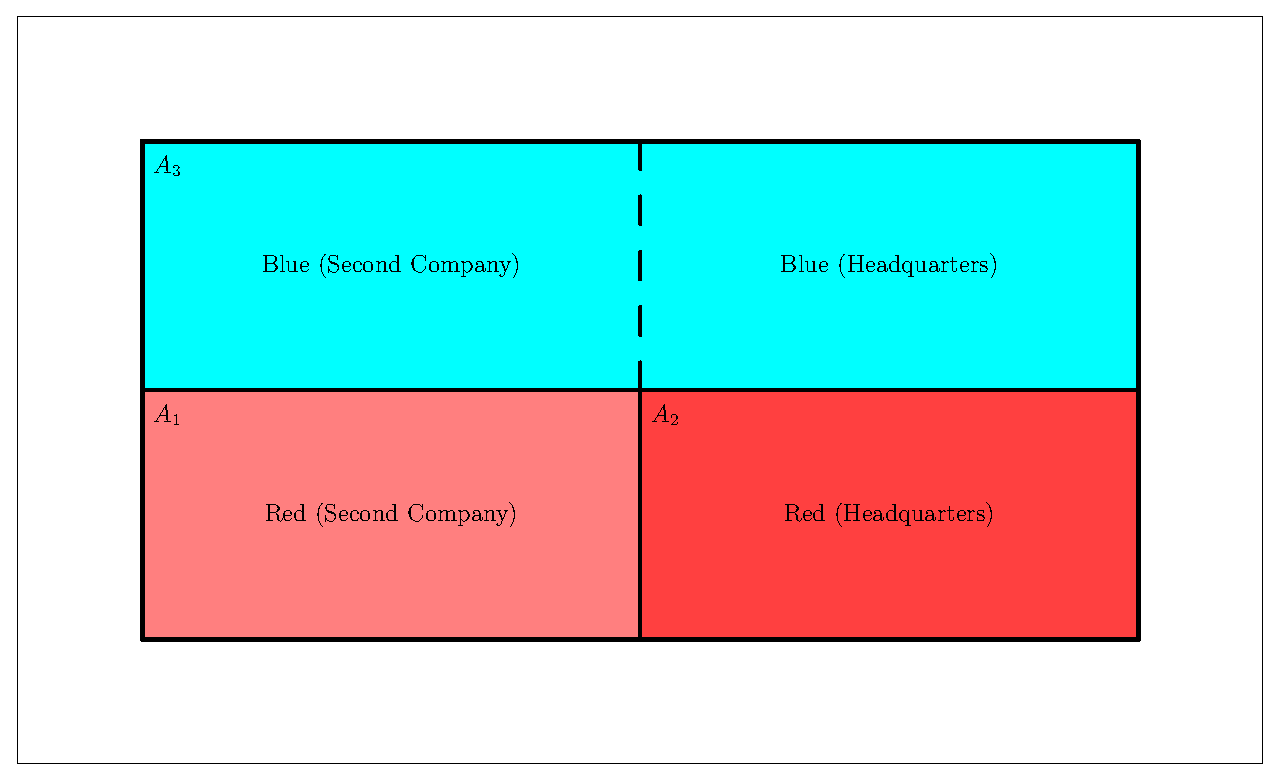
\includegraphics[width=\textwidth]{judy.eps}
      \caption{\footnotesize Judy Benjamin's map. Blue territory
        ($A_{3}$) is friendly and does not need to be divided into a
        Headquarters and a Second Company area.}
      \label{fig:map}
    \end{minipage}
\end{figure}

\begin{quotex}
  \beispiel{Judy Benjamin}\label{ex:judybenjamin} In van Fraassen's
  interpretation of the movie, Judy Benjamin is on an assignment and
  lands in a place where she is not sure of her location. She is on
  team Blue. Because of the map, initially the probability of being in
  Blue territory equals the probability of being in Red territory, and
  the probability of being in the Red Second Company area equals the
  probability of being in the Red Headquarters area. Her commanders
  then inform Judy by radio that in case she is in Red territory, her
  chance of being in the Red Headquarters area is three times the
  chance of being in the Red Second Company area.
\end{quotex}

The question is what Judy's appropriate response is to this new
evidence. We cannot apply standard conditioning, because there is no
immediately obvious event space in which we can condition on an event
of which we are certain. Grove and Halpern \scite{1}{grovehalpern97}{}
have offered a proposal for constructing such event spaces and then
conditioning on the event that Judy Benjamin receives the information
that she receives from her commanders. They admit, however, that the
construction of such spaces (sometimes called retrospective
conditioning) is an exercise in filling in missing details and
supplying information not contained in the original problem.

If we assume that the attempt fails to define an event on which Judy
Benjamin could condition her probabilities, we are left with two
possibilities. Her new information (it is three times as likely to
land in $A_{2}$ than to land in $A_{1}$, see {\igure}~\ref{fig:map} and
the details of the problem in the next section) may mean that we have
a redistribution of a complete partition of the probabilities. This is
called Jeffrey conditioning and calls for Jeffrey's rule. Jeffrey's
rule is contested in some circles, but we will for this project accept
its validity in probability kinematics. We will see in what follows
that some make the case that Jeffrey conditioning is the correct way
to solve the Judy Benjamin problem. For reasons provided in the body
of the chapter their case is implausible.

The third possibility to solve this problem (after standard
conditioning and Jeffrey conditioning) is to consult a highly
contested updating procedure: the principle of maximum entropy
(\textsc{pme} for short). \textsc{pme} can be applied to any
situation in which we have a completely quantified probability
distribution and an affine constraint (we will explain the nature of
affine constraints in more detail later). If our new evidence is the
observation of an event (or simply certainty about an event that we
did not have previously), then the event provides an affine constraint
and can be used for updating by means of standard conditioning. If our
new evidence is a redistribution of probabilities where we can apply
Jeffrey's rule, then the redistribution provides an affine constraint
and can be used for updating by means of Jeffrey's rule. These two
possibilities, however, do not exhaust affine constraints. The Judy
Benjamin problem illustrates the third possibility where the affine
constraint only redistributes some groups of probabilities and leaves
open the question how this will affect the probabilities not included
in this redistribution.

Advocates of \textsc{pme} claim that in this case the probabilities
should be adjusted so that they are minimally affected (we make this
precise by using information theory) while at the same time according
with the constraint. Opponents of this view grant that \textsc{pme}
is an important tool of probability kinematics. Noting that some
results of \textsc{pme} are difficult to accept (such as in the
Judy Benjamin case), however, they urge us to embrace a more
pluralistic, situation-specific methodology.

Joseph Halpern, for example, writes in \emph{Reasoning About
  Uncertainty} that \qeins{there is no escaping the need to understand
  the details of the application} \scite{2}{halpern03}{423} and
concludes that \textsc{pme} is a valuable tool, but should be used
with care (see \scite{8}{grovehalpern97}{110}), explicitly basing his
remark on the counterintuitive behaviour of the Judy Benjamin problem.
Diaconis and Zabell state \qeins{that any claims to the effect that
  maximum-entropy revision is the only correct route to probability
  revision should be viewed with considerable caution}
\scite{2}{diaconiszabell82}{829}. \qeins{Great caution} (1994,
456) is also what Colin Howson and Allan Franklin advise about
the more basic claim that the updated probabilities provided by
\textsc{pme} are as like the original probabilities as it is
possible to be given the constraints imposed by the data.

In the same vein, Igor Douven and Jan-Willem Romeijn agree with
Richard Bradley that \qeins{even Bayes' rule \qzwei{should not be
    thought of as a universal and mechanical rule of updating, but as
    a technique to be applied in the right circumstances, as a tool in
    what Jeffrey terms \emph{the art of judgment}.} In the same way,
  determining and adapting the weights {\ldots} may be an art, or a
  skill, rather than a matter of calculation or derivation from more
  fundamental epistemic principles} \scite{2}{douvenromeijn09}{16}
(for the Bradley quote see \scite{8}{bradley05}{362}).

What is lacking in the literature is a response by \textsc{pme}
advocates to the counterintuitive behaviour of the cases repeatedly
quoted by their adversaries. This is especially surprising as we are
not dealing with an array of counter-examples but only a handful, the
Judy Benjamin problem being prime among them. In Halpern's textbook,
for example, the reasoning is as follows: \textsc{pme} is a
promising candidate which delivers unique updated probability
distributions; but, unfortunately, there is counterintuitive behaviour
in one specific case, the Judy Benjamin case (see
\scite{8}{halpern03}{110, 119}); therefore, we must abide by the
eclectic principle of considering not only \textsc{pme}, but also
lower and upper probabilities, Dempster-Shafer belief functions,
possibility measures, ranking functions, relative likelihoods, and so
forth. The human inquirer is the final arbiter between these
conditionalization methods.

At the heart of our investigation are two incompatible but
independently plausible intuitions regarding Judy's choice of updated
probabilities for her location. We will undermine the notion that
\textsc{pme}'s solution for the Judy Benjamin problem is
counterintuitive. The intuition that \textsc{pme}'s solution for
the Judy Benjamin problem violates (call it T1) is based on fallacious
independence and uniformity assumptions. There is another powerful
intuition (call it T2) that conflicts with T1 and obeys
\textsc{pme}. Therefore, Halpern does not give us sufficient
grounds for the eclecticism advocated throughout his book. We will
show that another intuitive approach, the powerset approach, lends
significant support to the solution provided by \textsc{pme} for
the Judy Benjamin problem, especially in comparison to intuition T1,
many of whose independence and uniformity assumptions it shares. 

We have no proof that \textsc{pme} is the only rationally
defensible objective method to update probabilities given an affine
constraint. The literature outlines many of the \qnull{nice
  properties} of \textsc{pme}. It seamlessly generalizes standard
conditioning and Jeffrey's rule where they are applicable (see
\scite{7}{catichagiffin06}{}). It underlies the entropy concentration
phenomenon described in Jaynes' standard work \emph{Probability
  Theory: the Logic of Science}, which contains other arguments in
favour of \textsc{pme} (some of which you may recognize by family
resemblance in the rest of this chapter). Entropy concentration refers
to the unique property of \textsc{pme} solution to have other
distributions which obey the affine constraint cluster around it.
Shore and Johnston have shown that under certain rationality
assumptions \textsc{pme} provides the unique solution to problems
of probability updating (see \scite{7}{shorejohnson80}{}). When used
to make predictions whose quality is measured by a logarithmic score
functions, posterior probabilities provided by \textsc{pme} result
in minimax optimal decisions (see \scite{7}{topsoe79}{},
\scite{7}{walley91}{}, and \scite{7}{grunwald00a}{}). Under a
logarithmic scoring rule these posterior probabilities are in some
sense optimal.

Despite all these nice properties, we want the reader to follow us in
a more simple line of argument. When new evidence is provided to us,
it is rational to adjust our beliefs minimally in light of it. We do
not want to draw out more information from the new evidence than
necessary. We are the first to admit that there are numerous problems
here that need addressing. What do we mean by rationality? What are
the semantics of the word \qnull{minimal}? What are the formal
properties of such posterior probabilities? Are they unique? Are they
compatible with other intuitive methods of updating? Are there
counter-intuitive examples that would encourage us to give up on this
line of thought rather than live with its consequences? Given some
decent answers to these questions, however, we feel that
\textsc{pme} cuts a good figure as a first pass to provide
objective solutions to these types of problems, and the burden on
opponents who usually deny that there are such objective solutions
exist grows heavy.

The distinctive contribution of this chapter is to show why the
reasoning of the opponents of \textsc{pme} in the Judy Benjamin
case is flawed. They make independence assumptions that on closer
inspection do not hold up. We provide a number of scenarios consistent
with the information in the problem which violate these independence
assumptions. That does not mean that the information given in the
problem suggests these scenarios, it only means that we are not
entitled to make those independence assumptions. That, in turn, does
not privilege \textsc{pme} solution, although \textsc{pme}
does not lean on independence assumptions that other solutions
illegitimately make. \textsc{pme}, however, confronts us with a
much stronger claim than merely providing a passable or useful
solution to the Judy Benjamin problem: it claims to much greater
generality and, to use a term abjured by many formal epistemologists,
to objectivity. These claims must be motivated elsewhere, and the
nature of their normativity is a matter of debate (for a pragmatic
approach see \scite{7}{caticha12}{}). We are only showing that
opponents cannot claim an easy victory by pulling out old Judy
Benjamin.

There is a long-standing disagreement between (mostly) philosophers on
the one hand and (mostly) physicists on the other hand. The
philosophers claim that updating probabilities is irreducibly
accompanied by thoughtful deliberation with the choice between
different updating procedures depending on individual problems. The
physicists claim that problems are ill-posed if they do not contain
the information necessary to let a non-arbitrary, objective procedure
(such as \textsc{pme}) arrive at a unique updated probability
distribution. In the literature, Judy Benjamin serves as an example
widely taken to count in favour of the philosophers. It is taken to
support what I shall call the full employment theorem of probability
kinematics.

The full employment theorem of probability kinematics claims that
\textsc{pme} is only one of many different strategies to update
probabilities. In order to decide which strategy is the most
appropriate for your problem you need a resident formal epistemologist
to do the thinking and weigh the intuitions for you. For a fee, of
course. Thus formal epistemologists will always be fully employed. For
examples, see \scite{7}{seidenfeld86}{}; \scite{7}{grovehalpern97}{};
\scite{8}{halpern03}{54f} and 423; van Fraassen
\scite{10}{fraassen93}{306}; \scite{8}{neapolitanjiang14}{4012};
consider also Carnap's discussion, motivated by Alan Turing, of the
impossibility of an automatic inductive procedure in
\scite{8}{carnap62}{192--199}. E.T. Jaynes derisively talks about the
statistician-client relationship as one between a doctor and his
patient, see \scite{8}{jaynesbretthorst03}{492 and 506}. There is an
analogous full employment theory in computer science about writing
computer programs which has been formally proven to be true. Our
contention is that no such proof is forthcoming in probability
kinematics.

\section{Two Intuitions}
\label{sec:daingeum}

There are two pieces of information relevant to Judy Benjamin
when she decides on her updated probability assignment. We will call
them ({\ref{eq:map}}) and ({\ref{eq:hdq}}). As in
{\igure}~\ref{fig:map}, $A_{1}$ is the Red Second Company area, $A_{2}$ is
the Red Headquarters area, $A_{3}$ is Blue territory. Judy presumably
wants to be in Blue territory, but if she is in Red territory, she
would prefer their Second Company area (where enemy soldiers are not
as well-trained as in the Headquarters area).

\begin{enumerate}
\item[({\ref{eq:map}})] Judy has no idea where she is. Because of the
  map, her probability of being in Blue territory equals the
  probability of being in Red territory, and the probability of being
  in the Red Second Company area equals the probability of being in
  the Red Headquarters area.
\item[({\ref{eq:hdq}})] Her commanders inform Judy that in case she is in Red
  territory, her chance of being in their Headquarters area is three
  times the chance of being in their Second Company area.
\end{enumerate}

\nial In formal terms (sloppily writing $A_{i}$ for the event of Judy
being in $A_{i}$),

\begin{equation}
  \label{eq:map}
  2\cdot{}P(A_{1})=2\cdot{}P(A_{2})=P(A_{3})\tag{\mbox{MAP}}
\end{equation}

\begin{equation}
  \label{eq:hdq}
  {\qvu}=P(A_{2}|A_{1}\cup{}A_{2})=\frac{3}{4}\tag{\mbox{HDQ}}
\end{equation}

\nial ({\ref{eq:hdq}}) is partial information because in contrast to
the kind of evidence we are used to in Bayes' formula (such as
\qnull{an even number was rolled}), and to the kind of evidence needed
for Jeffrey's rule (where a partition of the whole event space and its
probability redistribution is required, not only $A_{1}\cup{}A_{2}$,
but see here the objections in \scite{7}{douvenromeijn09}{}), the
scenario suggests that Bayesian conditionalization and Jeffrey's rule
are inapplicable. We are interested in the most defensible updated
probability assignment(s) and will express them in the form of a
normalized odds vector $(q_{1},q_{2},q_{3})$, following van Fraassen
\scite{1}{fraassen81}{}. $q_{i}$ is the updated probability $Q(A_{i})$
that Judy Benjamin is in $A_{i}$. Let $P$ be the probability
distribution prior to the new observation and $p_{i}$ the individual
\qnull{prior} probabilities. These probabilities are not to be
confused with prior probabilities that precede any kind of
information. In the spirit of probability update, or probability
kinematics, we will for the rest of the article refer to prior
probabilities as probabilities prior to an observation and the
subsequent update. The $q_{i}$ sum to $1$ (this differs from van
Fraassen's canonical odds vector, which is proportional to the
normalized odds vector but has $1$ as its first element). We define

\begin{equation}
  \label{eq:aengaini}
  t=\frac{{\qvu}}{1-{\qvu}}
\end{equation}

\nial $t$ is the factor by which ({\ref{eq:hdq}}) indicates that
Judy's chance of being in $A_{2}$ is greater than being in $A_{1}$. In
Judy's particular case, $t=3$ and ${\qvu}=0.75$. Two intuitions guide
the way people think about Judy Benjamin's situation.

\begin{enumerate}
  \item[\textbf{T1}] ({\ref{eq:hdq}}) does not refer to Blue territory and
  should not affect $P(A_{3})$: $q_{3}=p_{3}(=0.50)$.
\end{enumerate}

\nial There is another, conflicting intuition (due to Peter Williams
via personal communication with van Fraassen, see
\scite{8}{fraassen81}{379}):

\begin{enumerate}
\item[\textbf{T2}] If the value of ${\qvu}$ approaches $1$ (in other words,
  $t$ approaches infinity) then $q_{3}$ should approach $2/3$ as the
  problem reduces to one of ordinary conditioning. ({\ref{eq:hdq}})
  would turn into \qnull{if you are in Red territory you are almost
    certainly in the Red Headquarters area.} Considering
  ({\ref{eq:map}}), $q_{3}$ should approach $2/3$. 
\end{enumerate}

\nial Continuity considerations pose a contradiction to T1. (These
considerations are strong enough that Luc Bovens uses them as an
assumption to solve Adam Elga's Sleeping Beauty problem by parity of
reasoning in \scite{7}{bovens10}{}.) To parse these conflicting
intuitions, we will introduce several methods to provide $G$, the
function that maps ${\qvu}$ to the appropriate normalized updated odds
vector $(q_{1},q_{2},q_{3})$. 

The first method is extremely simple and accords with intuition T1:
$G_{\mbox{{\tiny ind}}}({\qvu})=(0.5(1-{\qvu}),0.5{\qvu},0.5)$. In
Judy's particular case with $t=3$ the normalized odds vector is (ind
stands for independent):

\begin{equation}
  \label{eq:shipodei}
  G_{\mbox{{\tiny ind}}}(0.75)=(0.125,0.375,0.500)
\end{equation}

\nial Both Grove and Halpern \scite{1}{grovehalpern97}{} and Douven
and Romeijn \scite{1}{douvenromeijn09}{} make a case for this
distribution. Grove and Halpern use standard conditioning on the event
of the message being transmitted to Judy. Douven and Romeijn use
Jeffrey's rule (because they believe that T1 is in this case so strong
that $Q(A_{3})=P(A_{3})$ is as much of a constraint as (\ref{eq:map})
and (\ref{eq:hdq}), yielding a Jeffrey partition). 

T1, however, conflicts with the symmetry requirements outlined in van
Fraassen et.\ al.\ \scite{1}{fraassenetal86}{}. Van Fraassen
introduces various updating methods which do not conflict with those
symmetry requirements, the most notable of which is \textsc{pme}.
Shore and Johnson have already shown that, given certain assumptions
(which have been heavily criticized, e.g.\ in \scite{7}{uffink96}{}),
\textsc{pme} produces the unique updated probability assignment
according with these assumptions. The minimum information
discrimination theorem of Kullback and Leibler (see for example
\scite{7}{csiszar67}{}, section~3) demonstrates how Shannon's entropy
and the Kullback-Leibler Divergence formula can provide the least
informative updated probability assignment (with reference to the
prior probability assignment) obeying the constraint posed by the
evidence. The idea is to define a space of probability distributions,
make sure that the constraint identifies a closed, convex subset in
this space, and then determine which of the distributions in the
closed, convex subset is least distant from the prior probability
distribution in terms of information (using the minimum information
discrimination theorem). It is necessary for the uniqueness of this
least distant distribution that the subset be closed and convex (in
other words, that the constraint be affine, see
\scite{7}{csiszar67}{}).

For Judy Benjamin, \textsc{pme} suggests the following normalized
odds vector:

\begin{equation}
  \label{eq:vmax}
  G_{\mbox{{\tiny max}}}(0.75)\approx(0.117,0.350,0.533)
% use testgenq.m for this, see page 143 in Green Book
\end{equation}

{\noindent}The updated probability of being on Blue territory ($A_{3}$) has
increased from 50\% to approximately 53\%. Grove and Halpern find this
result \qeins{highly counterintuitive} \scite{2}{grovehalpern97}{2}.
Van Fraassen summarizes the worry:
\begin{quotex}
  It is hard not to speculate that the dangerous implications of being
  in the enemy's Headquarters area are causing Judy Benjamin to
  indulge in wishful thinking, her indulgence becoming stronger as her
  conditional estimate of the danger increases. \scite{3}{fraassen81}{379}
\end{quotex}

\bigskip

\nial There are two ways in which we can arrive at result
({\ref{eq:vmax}}). We may use Jaynes' constraint rule and find the
updated probability distribution that is both least informative with
respect to Shannon's entropy and in accordance with the constraint
(using Dempster's Rule of Combination, which together with the
constraint rule is equivalent to the principle of minimum
cross-entropy, see \scite{8}{coverthomas06}{409}, exercise 12.2.).
Alternatively, if circumstances are favourable (as they are in Judy
Benjamin's case), we may use the Kullback-Leibler Divergence and
differentiate it to obtain where it is minimal.

% addtorevisionbegin

The constraint rule has the advantage of providing results when the
derivative of the Kullback-Leibler Divergence is difficult to find.
This not being the case for Judy, we go the easier route of the second
method and provide a more general justification for the constraint
rule in subsection~\ref{subsec:choiwohk}, together with its
application to the Judy Benjamin case.

The Kullback-Leibler Divergence is

\begin{equation}
  \label{eq:gujeshoh}
  D(Q,P)=\sum_{i=1}^{m}q_{i}\log_{2}\frac{q_{i}}{p_{i}}.
\end{equation}

{\noindent}We fill in the explicit details from Judy Benjamin's situation and
differentiate the expression to obtain the minimum (by setting the
derivative to $0$). 

\begin{equation}
  \label{eq:ohyooquo}
\frac{\partial}{\partial{}q_{1}}(q_{1}\log_{2}(4q_{1})+tq_{1}\log_{2}(4tq_{1})+(1-(t+1)q_{1})\log_{2}2(1-(t+1)q_{1}))=0
\end{equation}

{\noindent}The resulting expression for $G_{\mbox{\tiny max}}$ is

\begin{equation}
  \label{eq:ahkoonae}
  G_{\mbox{\tiny max}}({\qvu})=\left(\frac{C}{1+Ct+C},t\frac{C}{1+Ct+C},1-(t+1)\frac{C}{1+Ct+C}\right),
\end{equation}

{\noindent}where

\begin{equation}
  \label{eq:johvulat}
  C=2^{-\frac{t\log_{2}t+t+1}{1+t}}.
\end{equation}

% addtorevisionend

Figures~\ref{fig:unif} and \ref{fig:mxnt} show in diagram form the
distribution of $(q_{1},q_{2},q_{3})$ depending on the value of ${\qvu}$
(between 0 and 1), respectively following intuition T1 and
\textsc{pme}. Notice that in accordance with intuition T2,
\textsc{pme} provides a result where $q_{3}\rightarrow{}2/3$ for
${\qvu}$ approaching 0 or 1.

\begin{figure}[ht!]
    \begin{minipage}[h]{.7\linewidth}
      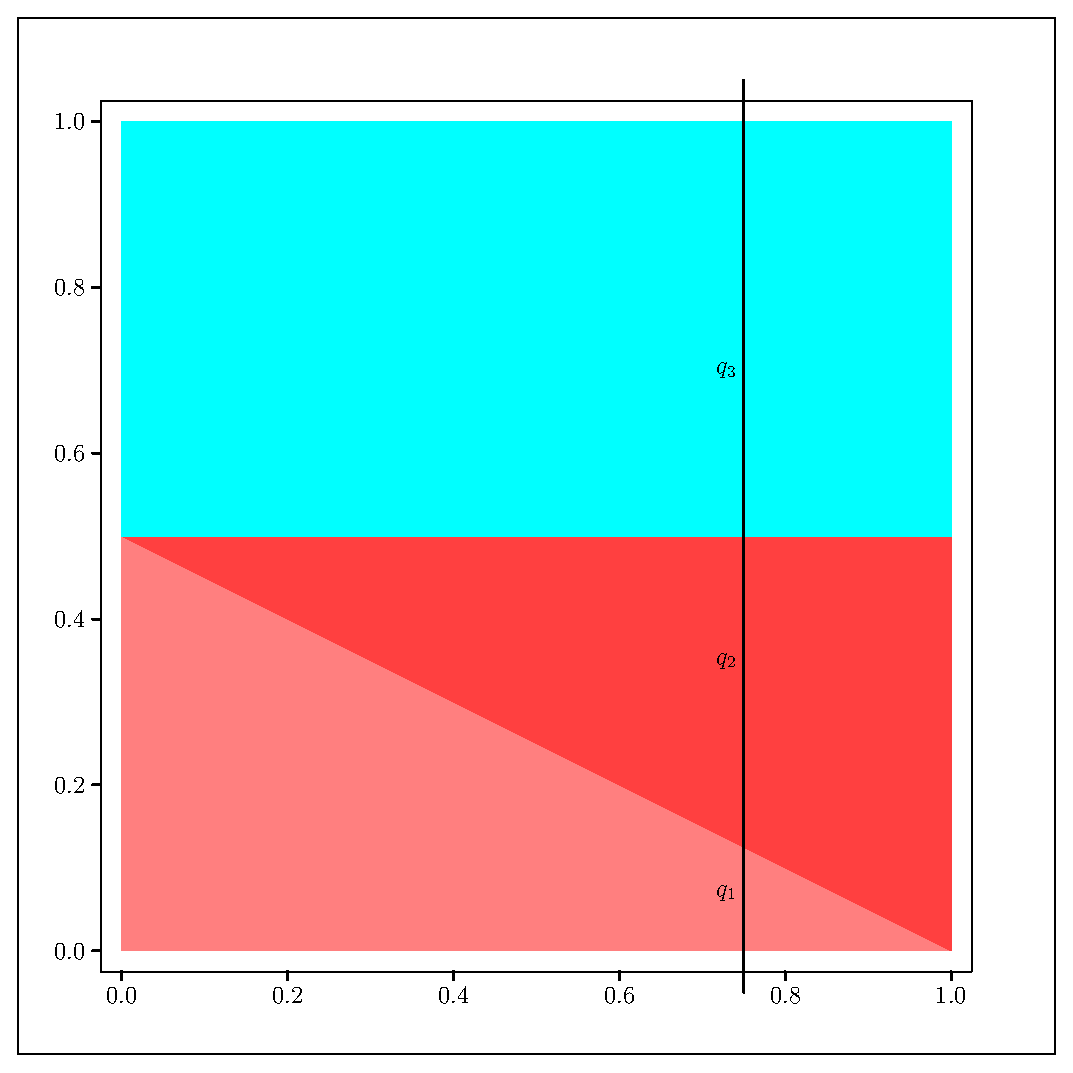
\includegraphics[width=\textwidth]{zeroone-unif.eps}
      \caption{\footnotesize Judy Benjamin's updated probability
        assignment according to intuition T1. $0<{\qvu}<1$ forms the
        horizontal axis, the vertical axis shows the updated
        probability distribution (or the normalized odds vector)
        $(q_{1},q_{2},q_{3})$. The vertical line at ${\qvu}=0.75$
        shows the specific updated probability distribution
        $G_{\mbox{\tiny ind}}(0.75)$ for the Judy Benjamin problem.}
      \label{fig:unif}
    \end{minipage}
\end{figure}

\begin{figure}[ht!]
    \begin{minipage}[h]{.7\linewidth}
      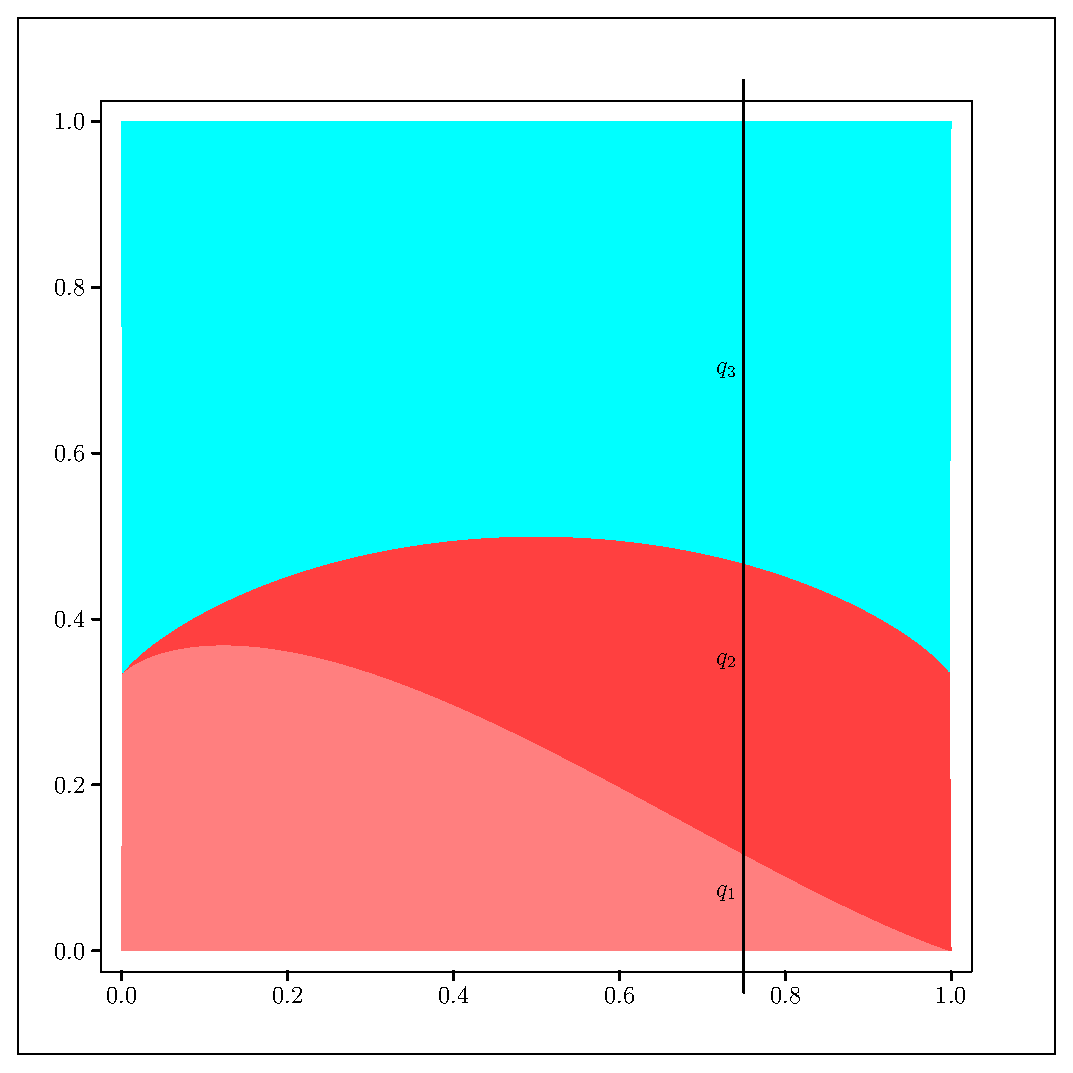
\includegraphics[width=\textwidth]{zeroone-mxnt.eps}
      \caption{\footnotesize Judy Benjamin's updated probability
        assignment using \textsc{pme}. $0<{\qvu}<1$ forms the
        horizontal axis, the vertical axis shows the updated
        probability distribution (or the normalized odds vector)
        $(q_{1},q_{2},q_{3})$. The vertical line at ${\qvu}=0.75$
        shows the specific updated probability distribution
        $G_{\mbox{\tiny max}}(0.75)$ for the Judy Benjamin problem.}
      \label{fig:mxnt}
    \end{minipage}
\end{figure}

\section{Epistemic Entrenchment}
\label{sec:oochaith}

Consider two future events $A$ and $B$. You have partial belief in
whether they will occur and assign probabilities to them. Then you
learn that $A$ entails $B$. How does this information affect your
probability assignment for event $A$? If $A$ is causally independent
of $B$ then your updated probability for it should equal the original
probability. 

\begin{quotex}
  \beispiel{Sundowners at the Westcliff}\label{ex:sundowners} Whether
  Sarah and Marian have sundowners at the Westcliff hotel tomorrow may
  initially not depend on the weather at all, but if they learn that
  there will be a wedding and the hotel's indoor facilities will be
  closed to the public, then rainfall tomorrow implies no
  sundowners.\label{page:oquohsae}
\end{quotex}

Learning this conditional does not affect the probability of the
antecedent (rainfall tomorrow), because the antecedent is causally
independent of the consequent.

\begin{quotex}
  \beispiel{Heist}\label{ex:jewelry} A jeweler has been robbed, and
  Kate has reason to assume that Henry might be the robber. Kate knows
  that he is not capable of actually injuring another person, but he
  may very well engage in robbery. When Kate hears from the
  investigator that the robber also shot the jeweler she concludes
  that Henry is not the robber. (A similar example is in Leendert
  Huisman's paper \qeins{Learning from Simple Indicative
    Conditionals,} to be published in \emph{Erkenntnis}, involving an
  exam and a skiing vacation.)
\end{quotex}

Kate has learned a conditional and adjusted the probability for the
antecedent. The reason for this is that Kate was epistemically
entrenched to uphold her belief in Henry's nonviolent nature. Updating
probabilities upon learning a conditional depends on epistemic
entrenchments. Examples \ref{ex:sundowners} and \ref{ex:jewelry} are
from \scite{7}{douvenromeijn09}{}).

In Judy Benjamin's case, (HDQ) is also a conditional. If Judy is in
Red territory, she is more likely to be in the Headquarters area.
According to \textsc{pme}, the updated probability for the
antecedent of this conditional is raised. It appears that
\textsc{pme} preempts our epistemic entrenchments and nolens volens
assigns a certain degree of confirmation to the antecedent of a
learned conditional. This degree of confirmation depends on the
causal dependency of the antecedent on the consequent. In this
section we will focus on the independence assumptions that are
improperly imported into the Judy Benjamin case by detractors of
\textsc{pme}. We will be particularly critical of Douven and
Romeijn, who hold that the Judy Benjamin case is a case for Adam's
conditioning, where the antecedent is left alone in the updating of
probabilities.

Even though T1 is an understandably strong intuition, it does
not take into account that the information given to Judy by her
commanders may indeed be dependent on whether she is in Blue or in Red
territory. To underline this objection to intuition T1 consider three
scenarios, any of which may form the basis of the partial information
provided by her commanders.

\begin{enumerate}
\item[\textbf{I}] Judy is dropped off by a pilot who flips two
  coins. If the first coin lands H, then Judy is dropped off in Blue
  territory, otherwise in Red territory. If the second coin lands H,
  she is dropped off in the Headquarters area, otherwise in the
  Second Company area. Judy's commanders find out that the second coin
  is biased ${\qvu}:1-{\qvu}$ toward H with ${\qvu}=0.75$. The normalized odds
  vector is $G_{\mbox{\tiny I}}(0.75)=(0.125,0.375,0.500)$ and agrees
  with T1, because the choice of Blue or Red is completely independent
  from the choice of the Red Headquarters area or the Red Second
  Company area.
\item[\textbf{II}] The pilot randomly lands in any of the four
  quadrants and rolls a die. If she rolls an even number, she drops
  off Judy. If not, she takes her to another (or the same, the choice
  happens with replacement) randomly selected quadrant to repeat the
  procedure. Judy's commanders find out, however, that for $A_{1}$,
  the pilot requires a six to drop off Judy, not just an even number.
  The normalized odds vector in this scenario is $G_{\mbox{\tiny
      II}}(0.75)=(0.1,0.3,0.6)$ and does not accord with T1.
\item[\textbf{III}] Judy's commanders have divided the map into $24$
  congruent rectangles, $A_{3}$ into twelve, and $A_{1}$ and $A_{2}$
  into six rectangles each (see figures~\ref{fig:pwstex1} and
  \ref{fig:pwstex2}). They have information that the only subsets of
  the $24$ rectangles in which Judy Benjamin may be located are such
  that they contain three times as many $A_{2}$ rectangles than
  $A_{1}$ rectangles. The normalized odds vector in this scenario is
  $G_{\mbox{\tiny III}}(0.75)\approx(.108,.324,.568)$ (evaluating almost
  17 million subsets).
\end{enumerate}

I--III demonstrate the contrast between scenarios when independence is
true and when it is not. Douven and Romeijn's capital mistake in their
paper is that they assume that the Judy Benjamin problem is analogous
to example \ref{ex:sundowners}. Sarah, however, knows that whether it
rains or not is independent of her activity the next night, whereas in
Judy Benjamin we have no evidence of such independence, as scenario II
makes clear. This is not to say that scenario II is the scenario that
pertains in Judy Benjamin's case. It only says that there is no
natural assumption in Judy Benjamin's case that the probabilities are
independent of each other in light of the new evidence, for scenario
II is perfectly natural (whether it is true or not is a completely
different question) and reveals how dependence is consistent with the
information that Judy Benjamin receives.

Douven and Romeijn's strong independence claim relying on intuition T1
leads them to apply Jeffrey's rule to the Judy Benjamin problem with
the additional constraint $q_{3}=p_{3}$. They claim that in most cases
\qeins{the learning of a conditional is or would be irrelevant to
  one's degree of belief for the conditional's antecedent {\ldots} the
  learning of the relevant conditional should intuitively leave the
  probability of the antecedent unaltered}
\scite{2}{douvenromeijn09}{9}.

This, according to Douven and Romeijn, is the usual epistemic
entrenchment and applies in full force to the Judy Benjamin problem.
They give an example where the epistemic entrenchment could go the
other way and leave the consequent rather than the antecedent
unaltered (Kate and Henry, see \scite{8}{douvenromeijn09}{13}). The
idea of epistemic entrenchment is at odds with \textsc{pme} and
seems to imply just what the full employment theorem claims: judgments
so framed \qeins{will depend on the judgmental skills of the agent,
  typically acquired not in the inductive logic class but by subject
  specific training} \scite{2}{bradley05}{349}. To pursue the
relation between the semantics of conditionals, \textsc{pme}, and
the full employment theorem would take us too far afield at present
and shall be undertaken elsewhere. For the Judy Benjamin problem, it
is not clear why Douven and Romeijn think that the way the problem is
posed implies a strong epistemic entrenchment for Adams conditioning
(Adams conditioning is the kind of conditioning that will leave the
antecedent alone). Scenarios II-III provide realistic alternatives
where Adams conditioning is inappropriate.

Judy Benjamin may also receive ({\ref{eq:hdq}}) because her informers
have found out that Red Headquarters troops have occupied the entire
Blue territory ($q_{1}=3p_{1},q_{2}=p_{2},q_{3}=0$, the epistemic
entrenchment is with respect to $q_{2}$); because they have found out
that Blue troops have occupied two-thirds of the Red Second Company
area ($q_{1}=p_{1},q_{2}=(1/3)p_{2},q_{3}=(4/3)p_{3}$, the epistemic
entrenchment is with respect to $q_{1}$); or because they have found
out that Red Headquarters troops have taken over half of the Red
Second Company area ($q_{1}=(1/2)p_{1},q_{2}=(3/2)p_{2},q_{3}=p_{3}$,
the epistemic entrenchment is with respect to $q_{3}$ and what Douven
and Romeijn take to be an assumption in the wording of the problem).
There is nothing in the problem that supports Douven and Romeijn's
narrowing of the options. The table reiterates these options, with the
third, shaded line representing intuition (T1) and the epistemic
entrenchment defended by Douven and Romeijn.

\begin{tabular}{|l|c|c|c|}\hline
Epistemic entrenchment & $q_{1}$ & $q_{2}$ & $q_{3}$ \\ \hline
with respect to $A_{1}$ & 1/4 & 3/4 & 0 \\ \hline
with respect to $A_{2}$ & 1/12 & 1/4 & 2/3 \\ \hline
with respect to $A_{3}$ & 1/8 & 3/8 & 1/2 \\ \hline
\end{tabular}

\section{Coarsening at Random}
\label{sec:ahdiesho}

Another at first blush forceful argument that \textsc{pme}'s solution
for the Judy Benjamin problem is counterintuitive has to do with
coarsening at random, or CAR for short. CAR involves using more naive
(or coarse) event spaces in order to arrive at solutions to
probability updating problems. The mechanics are spelled out in
\scite{1}{gruenwaldhalpern03}{}. Gr{\"u}nwald and Halpern see a
parallel between the Judy Benjamin problem and Martin Gardner's
\emph{Three Prisoners} problem, see {\xample} \ref{ex:threepris} on
page~\pageref{page:iabeiwet}.

% In the Three Prisoners problem, three men (A, B, and C) are under
% sentence of death when the governor decides to pardon one of them. The
% warden of the prison knows which of the three men is pardoned, but
% none of the men do. In a private conversation, A says to the warden,
% Tell me the name of one of the others who will be executed---it will
% not give anything away whether I will be executed or not. The warden
% agrees and tells A that B will be executed. For the puzzling
% consequences, see the wealth of literature on the Three Prisoners
% problem or the Monty Hall problem.

According to Gr{\"u}nwald and Halpern, for problems of this kind (Judy
Benjamin, Three Prisoners, Monty Hall) there are naive and
sophisticated spaces to which we can apply probability updates. If A
uses the naive space, for example, he comes to the following
conclusion: of the three possibilities that (A,B), (A,C), or (B,C) are
executed, the warden's information excludes (A,C). (A,B) and (B,C) are
left over, and because A has no information about which one of these
is true his chance of not being executed is 0.5. His chance of
survival has increased from one third to one half. 

Gr{\"u}nwald and Halpern show, correctly, that the application of the
naive space is illegitimate because the CAR condition does not hold.
More generally, Gr{\"u}nwald and Halpern show that updating on the
naive space rather than the sophisticated space is legitimate for
event type observations always when the set of observations is
pairwise disjoint or, when the events are arbitrary, only when the CAR
condition holds. For Jeffrey type observations, there is a generalized
CAR condition which applies likewise. For affine constraints on which
we cannot use Jeffrey conditioning (or, a fortiori, standard
conditioning) \textsc{maxent }\qeins{essentially never gives the right
  results} \scite{2}{gruenwaldhalpern03}{243}.

Gr{\"u}nwald and Halpern conclude that \qeins{working with the naive
  space, while an attractive approach, is likely to give highly
  misleading answers} (246), especially in the application of
\textsc{pme} to naive spaces as in the Judy Benjamin case
\qeins{where applying [\textsc{pme}] leads to paradoxical, highly
  counterintuitive results} (245). For the Three Prisoners problem,
Jaynes' constraint rule would supposedly proceed as follows: the
vector of prior probabilities for (A,B), (A,C), and (B,C) is
$(1/3,1/3,1/3)$. The constraint is that the probability of (A,C) is
zero, and a simple application of the constraint rule yields
$(1/2,0,1/2)$ for the vector of updated probabilities. The CAR
condition for the naive space does not hold, therefore the result is
misleading.

By analogy, using the constraint rule on the naive space for the Judy
Benjamin problem yields $(0.117,0.350,0.533)$, but as the CAR
condition fails in even the simplest settings for affine constraints
(\qeins{CAR is (roughly speaking) guaranteed \emph{not} to hold except
  in \qzwei{degenerate} situations} (251), emphasis in the original),
it certainly fails for the Judy Benjamin problem, for which
constructing a sophisticated space is complicated (see
\scite{7}{grovehalpern97}{}, where the authors attempt such a
construction by retrospective conditioning).

The analogy, however, is misguided. The constraint rule has been
formally shown to generalize Jeffrey conditioning, which in turn has
been shown to generalize standard conditioning (the authors admit as
much in \scite{8}{gruenwaldhalpern03}{262}). We can solve both the
Monty Hall problem and the Three Prisoners problem by standard
conditioning, not using the naive space, but simply using the correct
space for the probability update. For the Three Prisoners problem, for
example, the warden will say either \qnull{B} or \qnull{C} in response
to A's inquiry. Because A has no information that would privilege
either answer the probability that the warden says \qnull{B} and the
probability that the warden says \qnull{C} equal each other and
therefore equal 0.5. Here is the difference between using the naive
space and using the correct space, but either way using standard
conditional probabilities:
%  ($P'$ is the prior
% probability, before A receives the warden's information, $P''$ is the
% updated probability):

\begin{equation}
  \label{eq:ooshooth}
  \begin{array}{lcr}
    P(\mbox{`A is pardoned'}|\mbox{`B will be executed'})&=& \\
    \frac{P(\mbox{\footnotesize `A is pardoned'})}{P(\mbox{\footnotesize `A is
    pardoned'})+P(\mbox{\footnotesize `C is pardoned'})}&=&\frac{1}{2}\mbox{ (incorrect)} \\
  \end{array}
\end{equation}

\begin{equation}
  \label{eq:ailosahz}
  \begin{array}{lcr}
    P(\mbox{`A is pardoned'}|\mbox{`warden says B will be
    executed'})&=& \\
    \frac{P(\mbox{\footnotesize `A is pardoned' and `warden says B will
    be executed'})}{P(\mbox{\footnotesize `warden says B will be
    executed'})}&=&\frac{1/6}{1/2}=\frac{1}{3}\mbox{ (correct)} \\
  \end{array}
\end{equation}

\nial Why is the first equation incorrect and the second one correct?
Information theory gives us the right answer: in the first equation,
we are conditioning on a watered down version of the evidence (watered
down in a way that distorts the probabilities because we are not
\qnull{coarsening at random}). \qnull{Warden says B will be executed}
is sufficient but not necessary for \qnull{B will be executed.} The
former proposition is more informative than the latter proposition
(its probability is lower). Conditioning on the latter proposition
leaves out relevant information contained in the wording of the
problem.

Because \textsc{pme} always agrees with standard conditioning,
\textsc{pme} gives the correct result for the Three Prisoners
problem. For the Judy Benjamin problem, there is no defensible
sophisticated space and no watering down of the evidence in what
Gr{\"u}nwald and Halpern call the \qnull{naive} space. The analogy
between the Three Prisoners problem and the Judy Benjamin problem as
it is set up by Gr{\"u}nwald and Halpern fails because of this crucial
difference. A successful criticism would be directed at the
construction of the \qnull{naive} space: this is what we just
accomplished for the Three Prisoners problem. There is no parallel
procedure for the Judy Benjamin problem. The \qnull{naive} space is
all we have, and \textsc{pme} is the appropriate tool to deal with
this lack of information.

\section{The Powerset Approach}
\label{sec:eezaitod}

In this section, we will focus on scenario III and consider what
happens when the grain of the partition becomes finer. We call this
the powerset approach. Two remarks are in order. On the one hand, the
powerset approach has little independent appeal. The reason behind
using \textsc{pme} is that we want our evidence to have just the
right influence on our updated probabilities, i.e.\ neither
over-inform nor under-inform. There is no corresponding reason why we
should update our probabilities using the powerset approach. On the
other hand, what the powerset approach does is lend support to another
approach. In this task, it is persuasive because it tells us what
would happen if we were to divide the event space into infinitesimally
small, uniformly weighed, and independent \qnull{atomic} bits of
information.

In the process of arriving at the formal result, the powerset approach
resembles an empirical experiment. We are making many assumptions
favouring T1, but when the result comes in it supports T2 in
astonishingly non-trivial ways. The powerset approach provides support
for \textsc{pme} against T1 because it combines the assumptions
grounding T1 with a limit construction and still yields a solution
that closely approximates the one generated by \textsc{pme} rather
than the one generated by T1.

On its own the powerset approach is just what Gr{\"u}nwald and Halpern
call a naive space, for which CAR does not hold. Hence the powerset
approach will not give us a precise solution for the problem, although
it may with some plausibility guide us in the right
direction---especially if despite all its independence and uniformity
assumptions it significantly disagrees with intuition T1.

Let us assume a partition of the Blue and Red territories into sets of
equal measure (this is the division into rectangles of scenario III).
({\ref{eq:map}}) dictates that the number of sets covering $A_{3}$
equals the number of sets covering $A_{1}\cup{}A_{2}$. Initially, any
subset of this partition is a candidate for Judy Benjamin to consider.
The constraint imposed by ({\ref{eq:hdq}}) is that now we only
consider subsets for which there are three times as many partition
sets (or rectangles, although we are not necessarily limiting
ourselves to rectangles) in $A_{2}$ as there are in $A_{1}$. In
figures~\ref{fig:pwstex1} and \ref{fig:pwstex2} there are diagrams of
two subsets. One of them ({\igure}~\ref{fig:pwstex1}) is not a
candidate, the other one ({\igure}~\ref{fig:pwstex2}) is.

\begin{figure}[ht!]
    \begin{minipage}[h]{.7\linewidth}
      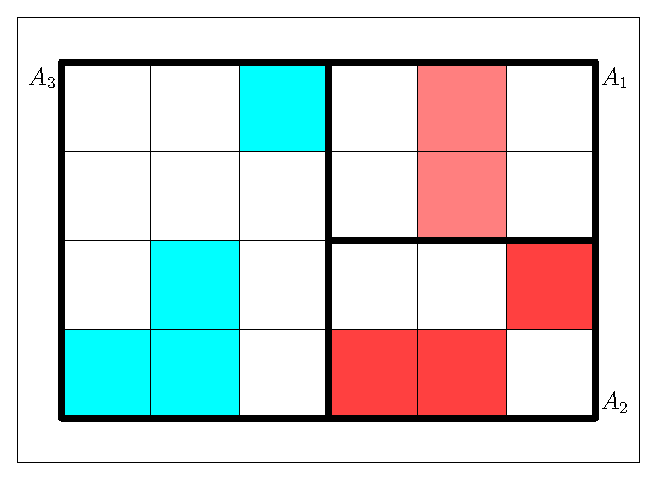
\includegraphics[width=\textwidth]{partition-2.eps}
      \caption{\footnotesize This choice of rectangles is not a
        candidate because the number of rectangles in $A_{2}$ is not a
        $t$-multiple of the number of rectangles in $A_{1}$, here with
        $s=2,t=3$ as in scenario III.}
      \label{fig:pwstex1}
    \end{minipage}
\end{figure}

\begin{figure}[ht!]
    \begin{minipage}[h]{.7\linewidth}
      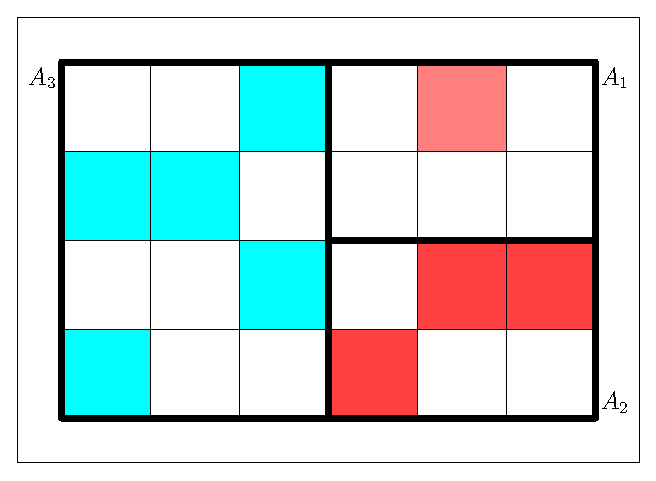
\includegraphics[width=\textwidth]{partition-1.eps}
      \caption{\footnotesize This choice of rectangles is a candidate
        because the number of rectangles in $A_{2}$ is a $t$-multiple
        of the number of rectangles in $A_{1}$, here with $s=2,t=3$ as
        in scenario III.}
      \label{fig:pwstex2}
    \end{minipage}
\end{figure}

Let $X$ be the random variable that corresponds to the ratio of the
number of partition elements (rectangles) that are in $A_{3}$ to the
total number of partition elements (rectangles) for a randomly chosen
candidate. We would now anticipate that the expectation of $X$ (which
we will call $EX$) gives us an indication of the updated probability
that Judy is in $A_{3}$ (so $EX\approx{}q_{3}$). The powerset approach
is often superior to the uniformity approach (Grove and Halpern use
uniformity, with all the necessary qualifications): if you have played
Monopoly, you will know that the frequencies for rolling a 2, a 7, or
a 10 with two dice tend to conform more closely to the binomial
distribution (based on a powerset approach) rather than to the uniform
distribution with $P(\mbox{rolling }i)=1/11$ for $i=2,{\ldots},12$.

Appendix~\ref{app:kiiwivul} provides a formula for the powerset
approach corresponding to the formula for \textsc{pme} approach,
giving us $q_{3}$ dependent on $t$. Notice that this formula is for
$t=2,3,4,\ldots$. For $t=1$ use the Chu-Vandermonde identity to find
that
\begin{equation}
  EX_{12}=(t+1)\frac{\sum_{i=1}^{s}i\binom{ts}{i}\binom{ts}{ti}}{\sum_{i=0}^{s}\binom{ts}{i}\binom{ts}{ti}}=(t+1)\frac{s}{2}  
\end{equation}
and consequently $EX=1/2$, as one would expect. For
$t=1/2,1/3,1/4,\ldots$ we can simply reverse the roles of $A_{1}$ and
$A_{2}$. These results give us $G_{\mbox{\tiny pws}}$ and a graph of
the normalized odds vector (see {\igure}~\ref{fig:pwst}), a bit bumpy
around the middle because the $t$-values are discrete and farther
apart in the middle, as $t={\qvu}/(1-{\qvu})$. Comparing the graphs of
the normalized odds vector under Grove and Halpern's uniformity
approach ($G_{\mbox{\tiny ind}}$), Jaynes' \textsc{pme} approach
($G_{\mbox{\tiny max}}$), and the powerset approach suggested in this
chapter ($G_{\mbox{\tiny pws}}$), it is clear that the powerset approach
supports \textsc{pme}.

\begin{figure}[ht!]
    \begin{minipage}[h]{.7\linewidth}
      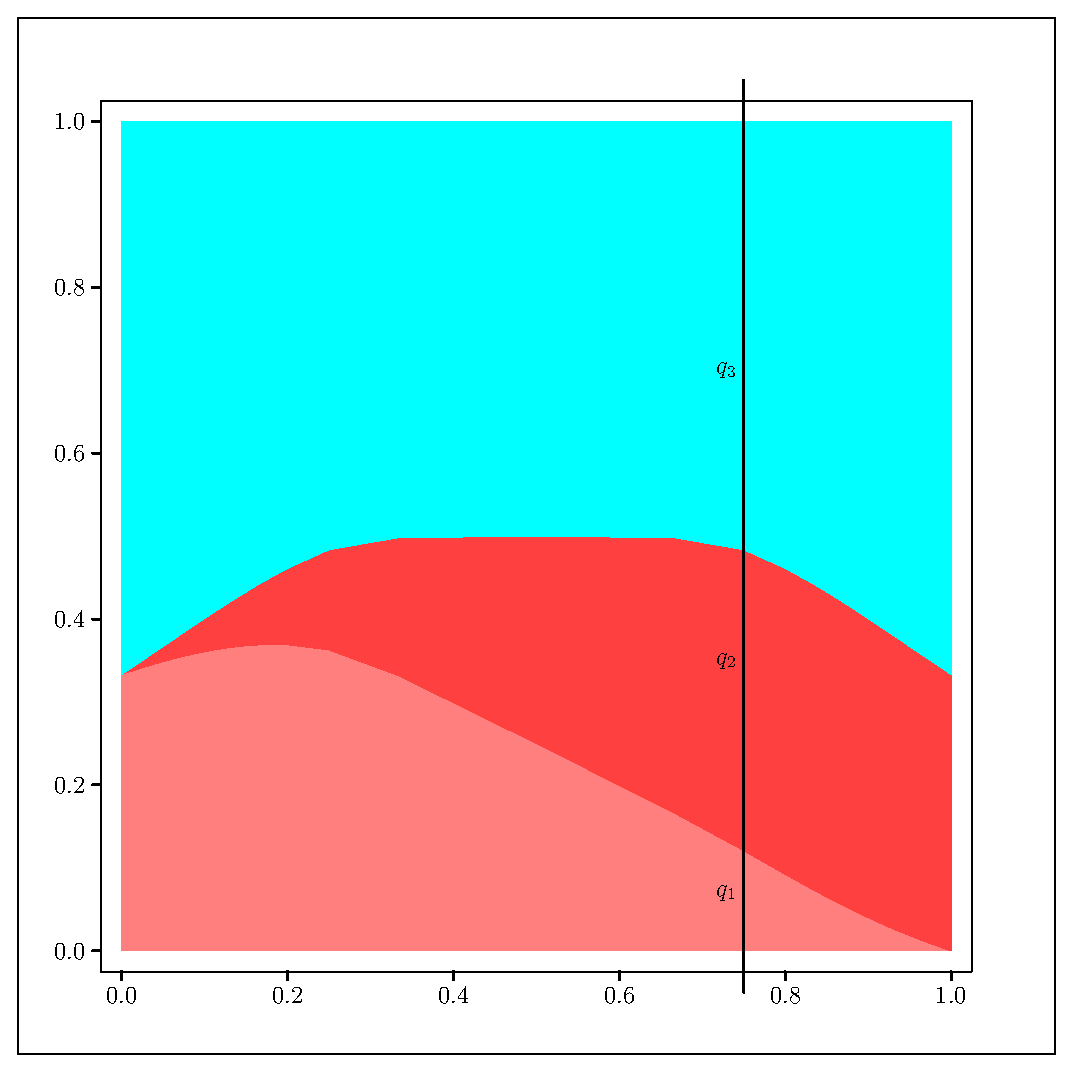
\includegraphics[width=\textwidth]{zeroone-pwst.eps}
      \caption{\footnotesize Judy Benjamin's updated probability
        assignment according to the powerset approach. $0<{\qvu}<1$
        forms the horizontal axis, the vertical axis shows the updated
        probability distribution (or the normalized odds vector)
        $(q_{1},q_{2},q_{3})$. The vertical line at ${\qvu}=0.75$
        shows the specific updated probability distribution
        $G_{\mbox{\tiny pws}}$ for the Judy Benjamin problem.}
      \label{fig:pwst}
    \end{minipage}
\end{figure}

Going through the calculations, it seems at many places that the
powerset approach should give its support to Grove and Halpern's
uniformity approach in keeping with intuition T1. It is unexpected to
find out that in the mathematical analysis the parameters converge to
a non-trivial factor and do not tend to negative or positive infinity.
Most surprisingly, the powerset approach, prima facie unrelated to an
approach using information, supports the idea that a set of events
about which nothing is known (such as $A_{3}$) gains in probability in
the updated probability distribution compared to the set of events
about which something is known (such as $A_{1}$ and $A_{2}$), even if
it is only partial information. Unless independence is specified, as
in example \ref{ex:sundowners}, the area of ignorance gains compared
to the area of knowledge.

We now have several ways to characterize Judy's updated
probabilities and updated probabilities following upon partial
information in general. Only one of them, the uniformity approach,
violates van Fraassen, Hughes, and Harman's five symmetry requirements
in \scite{1}{fraassenetal86}{} and intuition T2. The uniformity
approach, however, is the only one that satisfies intuition T1, an
intuition which most people have when they first hear the story. 

Two arguments attenuate the position of the uniformity approach in
comparison with the others. First, T1 rests on an independence
assumption which is not reflected in the problem. Although there is no
indication that what Judy's commanders tell her is in any way
dependent on her probability of being in Blue territory, it is not
excluded either (see scenarios II and III earlier in this chapter).
\textsc{pme} takes this uncertainty into consideration. Second,
when we investigate the problem using the powerset approach it turns
out that a division into equally probable, independent, and
increasingly fine bits of information supports not intuition T1 but
rather intuition T2. \textsc{pme}, for now, is vindicated. We need
to look for full employment not by cleverly manipulating prior
probabilities, but by making fresh observations, designing better
experiments, and partitioning the theory space more finely.

\chapter{Conclusion}
\label{chp:zeetahgh}

In this section the student must demonstrate his/her mastery of the
field and describe the work's overall contribution to the broader
discipline in context. A strong conclusion includes the following:

\begin{itemize}
\item Conclusions regarding the goals or hypotheses presented in the
  Introduction,
\item Reflective analysis of the research and its conclusions in light
  of current knowledge in the field,
\item Comments on the significance and contribution of the research
  reported,
\item Comments on strengths and limitations of the research,
\item Discussion of any potential applications of the research
  findings, and
\item A description of possible future research directions, drawing on
  the work reported.
\end{itemize}

% \bibliographystyle{apalike}
\bibliographystyle{ChicagoReedweb} 
\bibliography{bib-3415}

\appendix

\chapter{Weak Convexity and Symmetry in Information Geometry}
\label{app:wcs}

Using information theory instead of the geometry of reason, Joyce's
result still stands, vindicating probabilism on epistemic merits
rather than prudential ones: partial beliefs which violate probabilism
are dominated by partial beliefs which obey it, no matter what the
facts are.

Joyce's axioms, however, will need to be reformulated to accommodate
asymmetry. This appendix shows that the axiom Weak Convexity (see
section~\ref{sec:chuweiyo}) still holds in information geometry. Consider
three points $Q,R,S\in\mathbb{S}^{n-1}$ (replace $\mathbb{S}^{n-1}$ by the
$n$-dimensional space of non-negative real numbers, if you do not want
to assume probabilism) for which

\begin{equation}
  \label{eq:app1}
  D_{\mbox{\tiny KL}}(Q,R)=D_{\mbox{\tiny KL}}(Q,S).
\end{equation}

I will show something slightly stronger than Weak Convexity: Joyce's
inequality is not only true for the midpoint between $R$ and $S$ but
for all points $\vartheta{}R+(1-\vartheta)S$, as long as
$0\leq\vartheta\leq{}1$. The inequality aimed for is

\begin{equation}
  \label{eq:app2}
  D_{\mbox{\tiny KL}}(Q,\vartheta{}R+(1-\vartheta)S)\leq{}D_{\mbox{\tiny KL}}(Q,R)=D_{\mbox{\tiny KL}}(Q,S).
\end{equation}

{\noindent}To show that it holds I need the log-sum inequality, which is a result
of Jensen's inequality (for a proof of the log-sum inequality see
Theorem 2.7.1 in \scite{8}{coverthomas06}{31}). For non-negative
numbers $a_{1},\ldots,a_{n}$ and $b_{1},\ldots,b_{n}$,

\begin{equation}
  \label{eq:logsum}
  \sum_{i=1}^{n}a_{i}\ln\frac{a_{i}}{b_{i}}\geq\left(\sum_{i=1}^{n}a_{i}\right)\ln\frac{\sum_{i=1}^{n}a_{i}}{\sum_{i=1}^{n}b_{i}}.
\end{equation}

{\noindent}(\ref{eq:app2}) follows from (\ref{eq:logsum}) via

\begin{align}
  \label{eq:app3}
  &D_{\mbox{\tiny KL}}(Q,R)=\vartheta{}D_{\mbox{\tiny KL}}(Q,R)+(1-\vartheta)D_{\mbox{\tiny KL}}(Q,S)=\notag \\
  &\sum_{i=1}^{n}\left(\vartheta{}q_{i}\ln\frac{\vartheta{}q_{i}}{\vartheta{}r_{i}}+(1-\vartheta)q_{i}\ln\frac{(1-\vartheta)q_{i}}{(1-\vartheta)s_{i}}\right)\geq\notag \\
  &\sum_{i=1}^{n}q_{i}\ln\frac{q_{i}}{\vartheta{}r_{i}+(1-\vartheta)s_{i}}=D_{\mbox{\tiny KL}}(Q,\vartheta{}R+(1-\vartheta)S).
\end{align}

I owe some thanks to physicist friend Thomas Buchberger for help with
this proof. Interested readers can find a more general claim in
Csisz{\'a}r's Lemma 4.1 (see \scite{8}{csiszarshields04}{448}) which
accommodates convexity of the Kullback-Leibler divergence as a special
case.

\chapter{Asymmetry in Two Dimensions}
\label{app:asytwodims}

% See \texttt{http://math.stackexchange.com/questions/1428709/cant-swing-the-proof-for-this-inequality}.

This appendix contains a proof that the threefold partition
(\ref{eq:sieruxis}) of $\mathbb{S}^{1}$ is well-behaved, in contrast
to the threefold partition of $\mathbb{S}^{2}$ as illustrated by
{\igure}~\ref{fig:concat}. For the two-dimensional case, i.e.\
considering $p,q\in\mathbb{S}^{1}$ with $0<p,q<1, p+p'=1$ and
$q+q'=1$,

% \begin{align}
%   \label{eq:twodims}
%   \Delta_{q}(p)>0&\mbox{ for }&|p-p'|>|q-q'|\notag \\
%   \Delta_{q}(p)=0&\mbox{ for }&|p-p'|=|q-q'|\notag \\
%   \Delta_{q}(p)<0&\mbox{ for }&|p-p'|<|q-q'|
% \end{align}

\begin{equation}
  \label{eq:twodims}
  \begin{array}{rclcrcl}
  \Delta_{q}(p)&>&0&\mbox{ for }&|p-p'|&>&|q-q'|\\
  \Delta_{q}(p)&=&0&\mbox{ for }&|p-p'|&=&|q-q'|\\
  \Delta_{q}(p)&<&0&\mbox{ for }&|p-p'|&<&|q-q'|
  \end{array}
\end{equation}

{\noindent}where $\Delta_{q}(p)=D_{\mbox{\tiny KL}}(q,p)-D_{\mbox{\tiny
    KL}}(p,q)$ and $D_{\mbox{\tiny
    KL}}(p,q)=p\log\frac{p}{q}+(1-p)\log\frac{1-p}{1-q}$. Part of
information theory's ill behaviour outlined in section
\ref{subsec:Asymmetry} is that in the higher-dimensional case the
partition does not follow the simple rule that higher entropy of $P$
compared to $Q$ implies that $\Delta_{Q}(P)>0$ ($\Delta$ here defined
as in (\ref{eq:sksy})). In the two-dimensional case, however, this
simple rule applies. 

That a comparison in entropy $H(p)=-p\log{}p-(1-p)\log(1-p)$ between
$H(p)$ and $H(q)$ corresponds to a comparison of $|p-p'|$ and $|q-q'|$
is trivial. The proof for (\ref{eq:twodims}) is straightforward given
the following non-trivial lemma establishing a very tight inequality.
Given that $p+p'=1$ and $q+q'=1$ and $p,q,p',q'>0$ it is true
that

\begin{equation}
  \label{eq:lemma}
  \mbox{If }\log(p/q)>\log(q'/p')\mbox{ then }(p+q)\log(p/q)>(p'+q')\log(q'/p')
\end{equation}

{\noindent}Let $x=p/q$ and $y=q'/p'$. We know that $x>y$ since $\log{}x>\log{}y$.
Now we want to show $(p+q)\log{}x>(p'+q')\log{}y$. Note that
$p=xq,q'=p'y,p+q=q(x+1),$ and $p'+q'=p'(y+1)$. Therefore,

\begin{equation}
  \label{eq:thirteena}
  q=\frac{1-y}{1-xy}
\end{equation}

{\noindent}and

\begin{equation}
  \label{eq:thirteenb}
  p'=\frac{1-x}{1-xy}.
\end{equation}

{\noindent}What we want to show is that $x>y$ implies

\begin{equation}
  \label{eq:thirteenc}
  \frac{1-y}{1-xy}(x+1)\log{}x>\frac{1-x}{1-xy}\log{}y.
\end{equation}

{\noindent}Note that $f(x)=(1-x)^{-1}(x+1)\log{}x$ is increasing on $(0,1)$ and
decreasing on $(1,\infty{})$, and consider the following two cases:

(i) When $x<1,y<1$, (\ref{eq:thirteenc}) follows from the fact that
$f$ is increasing on $(0,1)$.

(ii) When $x>1,y>1$, (\ref{eq:thirteenc}) follows from the fact that
$f$ is decreasing on $(1,\infty)$.

{\noindent}Mixed cases such as $x>1,y<1$ do not occur, as for example $x>1$
implies $y>1$.

\begin{figure}[ht!]
    \begin{minipage}[h]{\linewidth}
      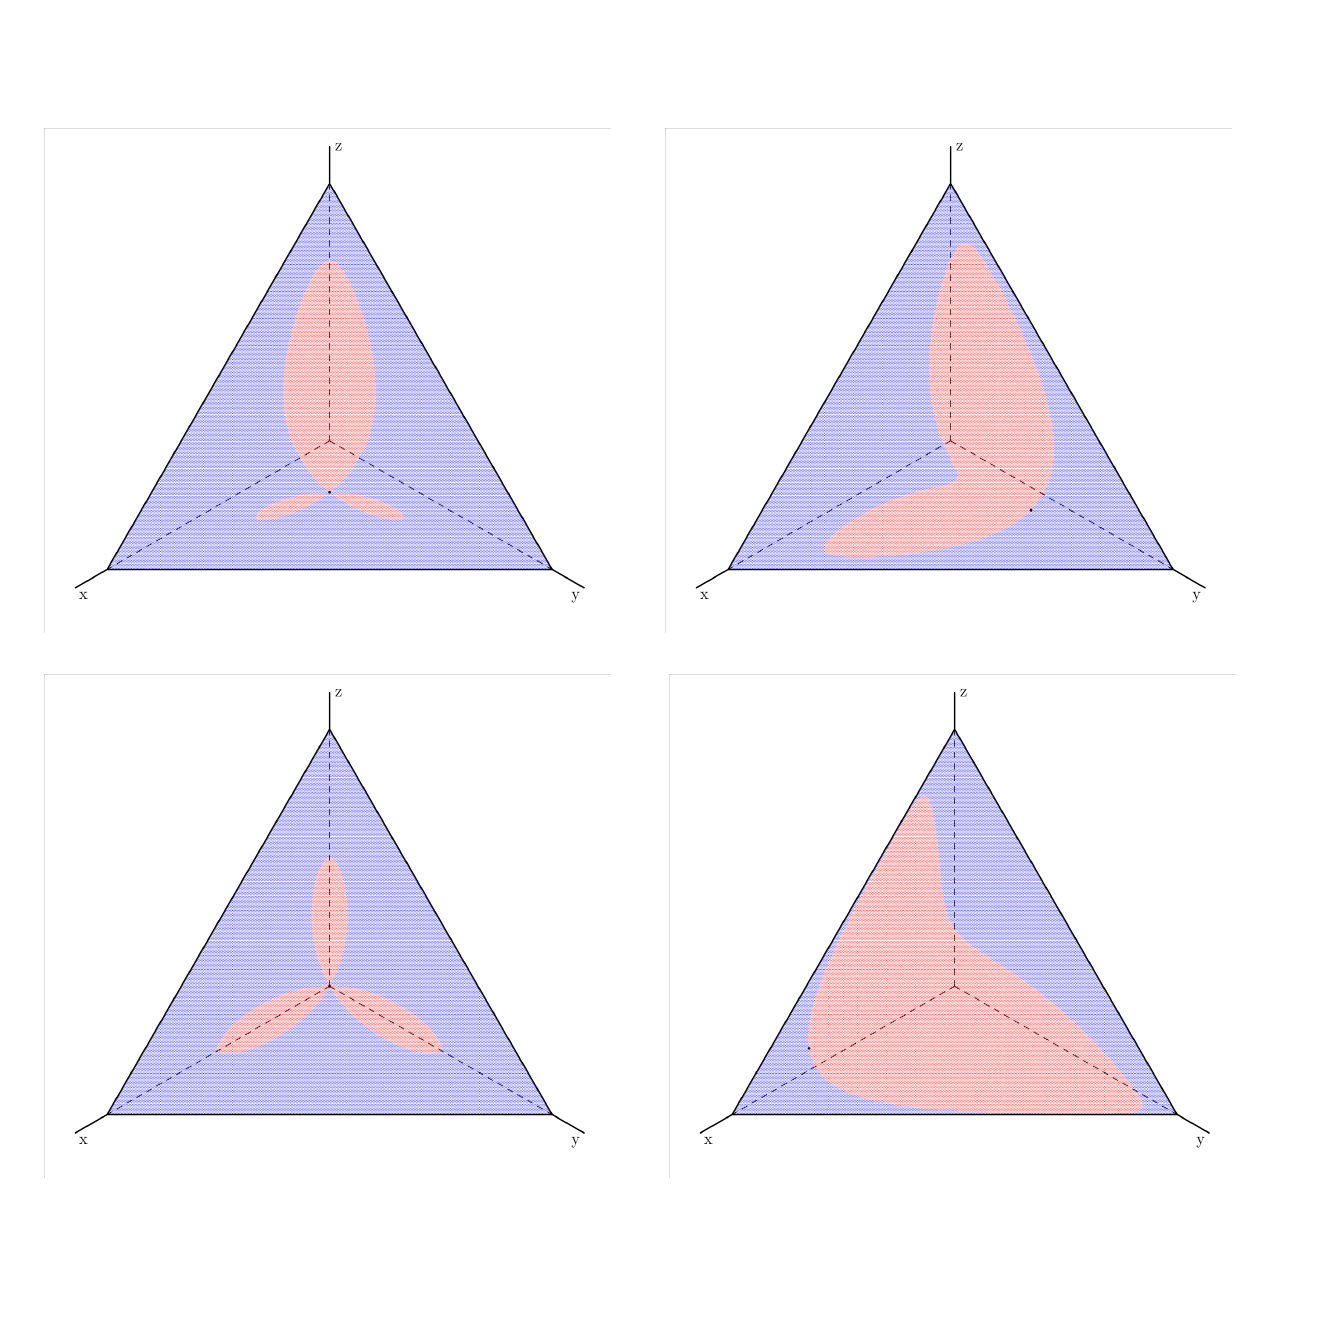
\includegraphics[width=\textwidth]{concat2.png}
      \caption{\footnotesize The partition (\ref{eq:sieruxis}) based
        on different values for $P$. From top left to bottom right,
        $P=(0.4,0.4,0.2); P=(0.242,0.604,0.154); P=(1/3,1/3,1/3);
        P=(0.741,0.087,0.172)$.
        Note that for the geometry of reason, the diagrams are
        trivial. The challenge for information theory is to explain
        the non-triviality of these diagrams epistemically without
        begging the question.}
      \label{fig:concat}
    \end{minipage}
\end{figure}

\chapter{The Horizon Requirement Formalized}
\label{app:horform}

Consider the following two conditions on a difference measure $D$ on a
simplex $\mathbb{S}^{n-1}\subset{}\mathbb{R}^{n}$, which is assumed to
be a smooth function from
$\mathbb{S}^{n-1}\times\mathbb{S}^{n-1}\rightarrow{}\mathbb{R}$.

\begin{enumerate}[(h1)]
\item If $p,p',q,q'$ are collinear with the centre of the
  simplex $m$ (whose coordinates are $m_{i}=1/n$ for all $i$) and an
  arbitrary but fixed boundary point $\xi\in\partial\mathbb{S}^{n-1}$
  and $p,p',q,q'$ are all between $m$ and $\xi$ with
  $\|p'-p\|=\|q'-q\|$ where $p$ is strictly closest to $m$, then
  $|D(p,p')|<|D(q,q')|$. For an illustration of this condition see
  {\igure}~\ref{fig:conditions}.
\item Let $\mu\in(-1,1)$ be fixed and $D_{\mu}$ defined as in
  (\ref{eq:defmu}). Then $dD_{\mu}/dx>0$, where $dD_{\mu}/dx$ is the
  total derivative as $x$ moves towards $\xi(x)$, the unique boundary
  point which is collinear with $x$ and $m$.
\end{enumerate}

To define $D_{\mu}$, the hardest part is to specify the domain. Let
this domain $V(\mu)\subseteq{}\mathbb{S}^{n-1}$ be defined as

\begin{equation}
  \label{eq:defvmu}
  V(\mu)=\left\{\begin{array}{ll}
    \{x\in\mathbb{S}^{n-1}|x_{i}<(1-\mu)\xi_{i}(x)+\mu{}m_{i},i=1,\ldots,n\}&\mbox{ for }\mu>0 \\
    \{x\in\mathbb{S}^{n-1}|x_{i}>(1+\mu)m_{i}-\mu{}\xi_{i}(x),i=1,\ldots,n\}&\mbox{ for }\mu<0.
  \end{array}\right.
\end{equation}

{\noindent}Then $D_{\mu}:V(\mu)\rightarrow{}\mathbb{R}^{+}_{0}$ is defined as

\begin{equation}
  \label{eq:defmu}
  D_{\mu}(x)=|D(x,y(x))|
\end{equation}

{\noindent}where $y_{i}(x)=x_{i}+\mu(\xi_{i}(x)-m_{i})$. Remember that $\xi(x)$
is the unique boundary point which is collinear with $x$ and $m$.
Now for the proof that (h1) and (h2) are equivalent. 

First assume (h1) and the negation of (h2). Since $D$ is smooth, there
must be a $\bar{\mu}$ and two points $x'$ and $x''$ collinear with $m$
and a boundary point $\bar{\xi}$ such that
$D_{\bar{\mu}}(x')\geq{}D_{\bar{\mu}}(x'')$ even though
$\|\bar{\xi}-x''\|<\|\bar{\xi}-x'\|$. If this were not the case,
$D_{\mu}$ would be strictly increasing running towards the boundary
points for all $\mu$ and its total derivative would be strictly
positive so that (h2) follows. Now consider the four points
$x',x'',y',y''$ where $y_{i}'=x_{i}'+\mu(\bar{\xi}_{i}-m_{i})$ and
$y_{i}''=x_{i}''+\mu(\bar{\xi}_{i}-m_{i})$ for $i=1,\ldots,n$. Without
loss of generality, assume $\bar{\mu}>0$. Then $x',x'',y',y''$ fulfill
the conditions in (h1) and $D_{\bar{\mu}}(x')<{}D_{\bar{\mu}}(x'')$,
in contradiction to the aforesaid.

Then assume (h2). Let $x',x'',y',y''$ be four points as in (h1).
Consider $\mu=\|\xi-m\|/\|x''-x'\|$. Then $D_{\mu}(x')=|D(x',x'')|$
and $D_{\mu}(y')=|D(y',y'')|$. (h2) tells us that along a path from
$m$ to $\xi$, $D_{\mu}$ is strictly increasing, so
$D_{\mu}(x')=|D(x',x'')|<|D(y',y'')|=D_{\mu}(y')$. QED.

Note that the Euclidean distance function violates both (h1) and (h2)
in all dimensions. The Kullback-Leibler divergence fulfills them if
$n=2$ but violates them if $n>2$. For $n=2$, this is easily checked by
considering the derivative of the Kullback-Leibler divergence for two
dimensions (use $D_{\varepsilon}$ defined in (\ref{eq:defdhpos}) and
(\ref{eq:defdhneg}) for the two-dimensional case instead of $D_{\mu}$
for the arbitrary-dimensional case). A counterexample to fulfillment
of (h1) and (h2) for $n=3$ is given in (\ref{eq:ubiesohx}).

Now that we have shown that (h1) and (h2) are equivalent, it is easy
to show that $J_{P},L_{P}$ and $Z_{P}$ fulfill the horizon requirement
while $M_{P},R_{P}$ and $G_{P}$ violate it. The following table of
derivatives will do (note that $\varepsilon=y-x$ is fixed while $x$
varies and that these derivatives have to be considered with the
absolute value for the various degree of confirmation functions in
mind). Column 1 is the name of the candidate confirmation function;
column 2 is the function with $x$ and $\varepsilon=y-x$ as arguments;
column 3 is the derivative $\partial{}D(x,\varepsilon)/\partial{}x$
for $|D(x,\varepsilon)|=D(x,\varepsilon)$.

\begin{tabular}{|l|l|l|}\hline
  $M_{P}(x,y)$ & $\displaystyle{}\varepsilon$ & $0$ \\ \hline
  $R_{P}(x,y)$ & $\displaystyle{}\log\frac{x+\varepsilon}{x}$ & $\displaystyle{}-\frac{\varepsilon}{(x+\varepsilon)x}$ \\ \hline
  $J_{P}(x,y)$ & $\displaystyle{}\frac{x+\varepsilon}{1-x-\varepsilon}-\frac{x}{1-x}$ & $\displaystyle{}\frac{1}{(1-x-\varepsilon)^{2}}-\frac{1}{(1-x)^{2}}$ \\ \hline
  $L_{P}(x,y)$ & $\displaystyle{}\log\frac{(x+\varepsilon)(1-x)}{x(1-x-\varepsilon)}$ & (\ref{eq:lpder}) \\ \hline
  $G_{P}(x,y)$ & $\displaystyle{}\log\frac{1-x}{1-x-\varepsilon}$ & $\displaystyle{}\frac{h}{(1-x)(1-x-\varepsilon}$ \\ \hline
  $Z_{P}(x,y)$ & $\displaystyle{}\frac{\varepsilon}{1-x}\mbox{ or }\frac{\varepsilon}{x}$ & $\displaystyle{}\frac{\varepsilon}{(1-x)^{2}}\mbox{ or }-\frac{\varepsilon}{x^{2}}$ \\ \hline
\end{tabular}

with

\begin{equation}
  \label{eq:lpder}
  -\frac{{\left({\left(x + \varepsilon\right)} {\left(1 - x\right)} - {\left(1 - x - \varepsilon\right)} x\right)} {\left(1-2x-\varepsilon\right)}}{{\left(x + \varepsilon\right)} {\left(1-x-\varepsilon\right)} {\left(1-x\right)} x}.
\end{equation}

\chapter{The Hermitian Form Model}
\label{app:eekiquom}

Asymmetric MDS is a promising approach to classify asymmetries in
terms of their behaviour. This subsection demonstrates that Chino's
asymmetric MDS, both spatial and non-spatial, fails to give us
explanations for information theory's violation of
\textsc{transitivity of asymmetry}. I am choosing Chino's approach
because it is the most general and most promising of all the different
asymmetric MDS models (see, for example, \scite{7}{chinoshiraiwa93}{},
where Chino manages to subsume many of the other approaches into his
own).

Multi-dimensional scaling (MDS) visualizes similarity of individuals
in data\-sets. Various techniques are used in information visualization,
in particular to display the information contained in a proximity
matrix. When the proximity matrix is asymmetrical, we speak of
asymmetric MDS. These techniques can be spatial (see for example
\scite{7}{chino78}{}), where the proximity relationships are
visualized in two-dimensional or higher-dimensional space; or
non-spatial (see for example \scite{7}{chinoshiraiwa93}{}), where the
proximity relationships are used to identify data sets with abstract
spaces (in Chino's case, finite-dimensional complex Hilbert spaces)
and metrics defined on them.

The spatial approach in two dimensions fails right away for
information theory because it cannot visualize transitivity
violations. The hope for other types of asymmetric MDS is that it
would be able to distinguish between well-behaved and ill-behaved
asymmetries and either exclude or identify better-behaved candidates
than the Kullback-Leibler divergence for measuring the distance
between probability distributions. I will use Chino's most
sophisticated non-spatial account to show that asymmetric MDS cannot
solve this problem. For other asymmetric MDS note that with the
Hermitian Form Model Chino seeks to integrate and generalize over all
the other accounts. 

Assume a finity proximity matrix. I will work with two examples here
to avoid the detailed and abstract account provided by Chino. The
first example is

\begin{equation}
  \label{eq:simpromat}
D=\left[
      \begin{array}{ccc}
        0 & 2 & 3 \\
        3 & 0 & 1 \\
        -1 & 2 & 0 
      \end{array}
\right]
\end{equation}

{\noindent}and allows for easy calculations. The second example corresponds to
(\ref{eq:transviol}), the example for transitivity violation where

\begin{equation}
  \label{eq:dklpromat}
\hat{D}=\left[
      \begin{array}{ccc}
0.0000 &  0.0566 &  0.0487 \\
0.0589 &  0.0000 &  0.0499 \\
0.0437 &  0.0541 &  0.0000
      \end{array}
\right],
\end{equation}

{\noindent}and the elements of the matrix $\hat{d}_{jk}=D_{\mbox{\tiny KL}}(P_{j},P_{k})$.
Note that the diagonal elements are all zero, as no updating is
necessary to keep the probability distribution constant.

Chino first defines a symmetric matrix $S$ and a skew-symmetric matrix
$T$ corresponding to the proximity matrix such that $D=S+T$.

\begin{equation}
  \label{eq:skewsym}
  S=\frac{1}{2}(D+D')\mbox{ and }T=\frac{1}{2}(D-D').
\end{equation}

{\noindent}Note that $D'$ is the transpose of $D$, $S$ is a symmetric matrix, and
$T$ is a skew-symmetric matrix with $t_{jk}=-t_{kj}$. Next we define
the Hermitian matrix

\begin{equation}
  \label{eq:herm}
  H=S+iT,
\end{equation}

{\noindent}where $i$ is the imaginary unit. $H$ is a Hermitian matrix with
$h_{jk}=\overline{h_{kj}}$. Hermitian matrices are the complex
generalization of real symmetric matrices. They have special
properties (see section~8.9 in \scite{7}{antonbusby03}{}) which
guarantee the existence of a unitary matrix $U$ such that

\begin{equation}
  \label{eq:unitary}
  H=U\Lambda{}U^{*},
\end{equation}

{\noindent}where $\Lambda=\mbox{diag}(\lambda_{1},\ldots,\lambda_{n})$ with $n$
the dimension of $D$ and $\lambda_{k}$ the $k$-th eigenvalue of $H$
(theorem 8.9.8 in \scite{7}{antonbusby03}{}). $U$ is the matrix of
eigenvectors with the $k$-th column being the $k$-th eigenvector.
$U^{*}$ is the conjugate transpose of $U$. Given example
(\ref{eq:simpromat}), the numbers look as follows:

\begin{equation}
  \label{eq:simh}
H=\frac{1}{2}\left[
      \begin{array}{ccc}
        0 & 5-i & 2+4i \\
        5+i & 0 & 3-i \\
        2-4i & 3+i & 0 
      \end{array}
\right]
\end{equation}

{\noindent}and

\begin{equation}
  \label{eq:simu}
U=\left[
      \begin{array}{ccc}
   0.019 + 0.639i & -0.375 + 0.195i &  0.514 + 0.386i \\
   0.279 - 0.494i & -0.169 - 0.573i &  0.503 + 0.260i \\
  -0.519 + 0.000i &  0.681 - 0.000i &  0.516 + 0.000i
      \end{array}
\right]
\end{equation}

{\noindent}with $\Lambda=\mbox{diag}(-3.78,0.0715,3.71)$. $\Lambda$ is
calculated using the characteristic polynomial
$\lambda^{3}-14\lambda+1$ of $H$. Notice that the characteristic
polynomial is a depressed cubic (the second coefficient is zero),
which facilitates computation and will in the end spell the failure of
Chino's program for our purposes.

Given {\xample}~(\ref{eq:dklpromat}), the numbers are
 
\begin{equation}
  \label{eq:dklh}
\hat{H}=\frac{1}{2}\left[
      \begin{array}{ccc}
   0.0000 + 0.0000i &  0.0578 - 0.0011i &  0.046 + 0.003i \\
   0.0578 + 0.0011i &  0.0000 + 0.0000i &  0.052 - 0.002i \\
   0.0462 - 0.0025i &  0.0520 + 0.0021i &  0.000 + 0.000i
      \end{array}
\right]
\end{equation}

{\noindent}and

\begin{equation}
  \label{eq:dklu}
\hat{U}=\left[
      \begin{array}{ccc}
   0.351 - 0.467i & -0.543 + 0.170i & -0.578 - 0.006i \\
  -0.604 + 0.457i & -0.201 - 0.169i & -0.598 + 0.002i \\
   0.290 - 0.000i &  0.779 + 0.000i & -0.555 + 0.000i
      \end{array}
\right]
\end{equation}

{\noindent}with $\Lambda=\mbox{diag}(-0.060,-0.045,0.104)$. 

Chino now elegantly shows how the decomposition of $H=U\Lambda{}U^{*}$
defines a seminorm on a vector space. Let
$\phi(\zeta,\tau)=\zeta\Lambda\tau^{*}$. Then (i)
$\phi(\zeta_{1}+\zeta_{2},\tau)=\phi(\zeta_{1},\tau)+\phi(\zeta_{2},\tau)$,
(ii) $\phi(a\zeta,\tau)=a\phi(\zeta,\tau)$, and (iii)
$\phi(\zeta,\tau)=\overline{\phi(\tau,\zeta)}$. These three conditions
characterize an inner product on a finite-dimensional complex Hilbert
space, but only if a fourth condition is met: positive (or negative)
definiteness ($\phi(\zeta,\zeta)\geq{}0)$ for all $\zeta$). One might
hope that positive definiteness identifies the more well-behaved
asymmetries by associating with them a finite-dimensional complex
Hilbert space with the norm $\|\zeta\|=\sqrt{\phi(\zeta,\zeta)}$
defined on it (Chino himself speculatively mentioned this hope to me
in personal communication).

The hope does not come to fruition. Without a non-trivial
self-similarity relation, all seminorms defined as above are
indefinite, and thus all cats grey in the night. Not only are
well-behaved and ill-behaved asymmetries indistinguishable by the
light of this seminorm, even the seminorms for symmetry are
indefinite. Not only does this not help our programme, it also puts a
serious damper on Chino's, who never mentions the self-similarity
requirement (which, given that we are dealing with a proximity matrix,
is substantial).

Based on a theorem in linear algebra (see theorem 4.4.12 in
\scite{7}{antonbusby03}{}),

\begin{equation}
  \label{eq:linalgtheorem}
    \sum_{j=1}^{n}\lambda_{j}=\mbox{tr}(A)
\end{equation}

{\noindent}whenever the $\lambda_{j}$ are the eigenvalues of $A$. The reader can
easily verify this theorem by noticing that the roots of the
characteristic polynomial add up to the second coefficient (which is
the trace of the original matrix). It is well-known that the
eigenvalues of a Hermitian matrix are real-valued (theorem 8.9.4 in
\scite{7}{antonbusby03}{}), which is an important component for Chino
to define the seminorm $\|\zeta\|$ with the help of $\phi$.
Unfortunately, using (\ref{eq:linalgtheorem}), the eigenvalues are not
only real, but also add up to the trace of $H$, which is zero unless
there is a non-trivial self-similarity relation.

Tversky entertains such self-similarity relations in psychology (see
\scite{8}{tversky77}{328}), and Chino is primarily interested in
applications in psychology. When the eigenvalues add up to zero,
however, there will be positive and negative eigenvalues (unless the
whole proximity matrix is the null-matrix), which renders the seminorm
as defined by Chino indefinite. The Kullback-Leibler divergence is
trivial with respect to self-similarity: $D_{\mbox{\tiny KL}}(P,P)=0$
for all $P$.

\chapter{The Powerset Approach Formalized}
\label{app:kiiwivul}

Let us assume a partition $\{B_{i}\}_{i=1,{\ldots},4n}$ of
$A_{1}\cup{}A_{2}\cup{}A_{3}$ into sets that are of equal measure
$\mu$ and whose intersection with $A_{i}$ is either the empty set or
the whole set itself (this is the division into rectangles of scenario
III). ({\ref{eq:map}}) dictates that the number of sets covering
$A_{3}$ equals the number of sets covering $A_{1}\cup{}A_{2}$. For
convenience, we assume the number of sets covering $A_{1}$ to be $n$.
Let $\mathcal{C}$, a subset of the powerset of
$\{B_{i}\}_{i=1,{\ldots},4n}$, be the collection of sets which agree
with the constraint imposed by ({\ref{eq:hdq}}), i.e.\
\begin{equation}
  \label{eq:iengiebu}
  C\in\mathcal{C}\mbox{ iff }C=\{C_{j}\}\mbox{ and }t\mu\left(\bigcup{}C_{j}\cap{}A_{1}\right)=\mu\left(\bigcup{}C_{j}\cap{}A_{2}\right)
\end{equation}
In figures~\ref{fig:pwstex1} and \ref{fig:pwstex2} there are diagrams
of two elements of the powerset of $\{B_{i}\}_{i=1,{\ldots},4n}$. One
of them ({\igure}~\ref{fig:pwstex1}) is not a member of $\mathcal{C}$,
the other one ({\igure}~\ref{fig:pwstex2}) is.

The binomial distribution dictates the expectation $EX$ of $X$, using
simple combinatorics. In this case we require, again for convenience,
that $n$ be divisible by $t$ and the \qnull{grain} of the partition
$A$ be $s=n/t$. Remember that $t$ is the factor by which
({\ref{eq:hdq}}) indicates that Judy's chance of being in $A_{2}$ is
greater than being in $A_{1}$. In Judy's particular case, $t=3$ and
${\qvu}=0.75$. We introduce a few variables which later on will help
for abbreviation:

\begin{equation}
  \label{eq:naibepha}
n=ts\hspace{.5in}
2m=n\hspace{.5in}
2j=n-1\hspace{.5in}
{T}=t^{2}+1
\end{equation}

$EX$, of course, depends both on the grain of $A$ and the value of
$t$. It makes sense to make it independent of the grain by letting the
grain become increasingly finer and by determining $EX$ as
$s\rightarrow\infty$. This cannot be done for the binomial
distribution, as it is notoriously uncomputable for large numbers
(even with a powerful computer things get dicey around $s=10$). But,
equally notorious, the normal distribution provides a good
approximation of the binomial distribution and will help us arrive at
a formula for $G_{\mbox{\tiny pws}}$ (corresponding to 
$G_{\mbox{\tiny ind}}$ and $G_{\mbox{\tiny max}}$), determining the value $q_{3}$
dependent on ${\qvu}$ as suggested by the powerset approach.

First, we express the random variable $X$ by the two independent
random variables $X_{12}$ and $X_{3}$. $X_{12}$ is the number of
partition elements in the randomly chosen $C$ which are either in
$A_{1}$ or in $A_{2}$ (the random variable of the number of partition
elements in $A_{1}$ and the random variable of the number of partition
elements in $A_{2}$ are decisively not independent, because they need
to obey ({\ref{eq:hdq}})); $X_{3}$ is the number of partition elements
in the randomly chosen $C$ which are in $A_{3}$. A relatively simple
calculation shows that $EX_{3}=n$, which is just what we would expect
(either the powerset approach or the uniformity approach would give us
this result):
\begin{equation}
  \label{eq:kuquoosu}
  EX_{3}=2^{-2n}\sum_{i=0}^{2n}i\binom{2n}{i}=n\mbox{ (use }\binom{n}{k}=\frac{n}{k}\binom{n-1}{k-1}\mbox{)}
\end{equation}

{\noindent}The expectation of $X$, $X$ being the random variable
expressing the ratio of the number of sets covering $A_{3}$ and the
number of sets covering $A_{1}\cup{}A_{2}\cup{}A_{3}$, is
\begin{equation}
  \label{eq:jahbohgh}
  EX=\frac{EX_{3}}{EX_{12}+EX_{3}}=\frac{n}{EX_{12}+n}
\end{equation}

If we were able to use uniformity and independence, $EX_{12}=n$ and
$EX=1/2$, just as Grove and Halpern suggest (although their uniformity
approach is admittedly less crude than the one used here). Will the
powerset approach concur with the uniformity approach, will it support
the principle of maximum entropy, or will it make another suggestion
on how to update the prior probabilities? To answer this question, we
must find out what $EX_{12}$ is, for a given value $t$ and
$s\rightarrow\infty$, using the binomial distribution and its
approximation by the normal distribution.

Using combinatorics,
\begin{equation}
  \label{eq:idooyeib}
  EX_{12}=(t+1)\frac{\sum_{i=1}^{s}i\binom{ts}{i}\binom{ts}{ti}}{\sum_{i=0}^{s}\binom{ts}{i}\binom{ts}{ti}}
\end{equation}

{\noindent}Let us call the numerator of this fraction NUM and the denominator
DEN. According to the de Moivre-Laplace Theorem,
\begin{equation}
  \label{eq:uumavael}
  \mbox{DEN}=\sum_{i=0}^{s}\binom{ts}{i}\binom{ts}{ti}\approx{}2^{2n}\sum_{i=0}^{s}\int_{i-\frac{1}{2}}^{i+\frac{1}{2}}\mathcal{N}(\frac{n}{2},\frac{n}{4})(i)\mathcal{N}(\frac{n}{2},\frac{n}{4})(ti)di
\end{equation}
where
\begin{equation}
  \label{eq:shiewain}
  \mathcal{N}(\mu,\sigma^{2})(x)=\frac{1}{\sqrt{2\pi\sigma^{2}}}\exp\left(-\frac{(x-\mu)^{2}}{2\sigma^{2}}\right)
\end{equation}
Substitution yields
\begin{equation}
  \label{eq:wahweele}
  \mbox{DEN}\approx{}2^{2n}\frac{1}{\pi{}m}\sum_{i=0}^{s}\int_{i-\frac{1}{2}}^{i+\frac{1}{2}}\exp\left(-\frac{\left(x-m\right)^{2}}{m}-\frac{t^{2}\left(x-\frac{m}{t}\right)^{2}}{m}\right)dx
\end{equation}
Consider briefly the argument of the exponential function:
\begin{equation}
  \label{eq:augahghu}
  -\frac{\left(x-m\right)^{2}}{m}-\frac{t^{2}\left(x-\frac{m}{t}\right)^{2}}{m}=-\frac{t^{2}}{m}({\aden}x^{2}+{\bden}x+{\cden})=-\frac{t^{2}}{m}\left({\aden}(x-{\hden})^{2}+{\kden}\right)
\end{equation}
with (the double prime sign corresponds to the simple prime sign for
the numerator later on)
\begin{equation}
  \label{eq:aiphueri}
{\aden}=\frac{1}{t^{2}}{T}\notag\hspace{.5in}
{\bden}=(-2m)\frac{1}{t^{2}}(t+1)\hspace{.5in}
{\cden}=2m^{2}\frac{1}{t^{2}}
\end{equation}
\begin{equation}
  \label{eq:quoseoth}
{\hden}=-{\bden}/2{\aden}\hspace{.5in}
{\kden}={\aden}{\hden}^{2}+{\bden}{\hden}+{\cden}
\end{equation}
Consequently,
\begin{equation}
  \label{eq:sheyupei}
\mbox{DEN}\approx{}2^{2n}\exp\left(-\frac{t^{2}}{m}{\kden}\right)\sqrt{\frac{1}{\pi{}{\aden}mt^{2}}}\int_{-\infty}^{s+\frac{1}{2}}\mathcal{N}\left({\hden},\frac{m}{2{\aden}t^{2}}\right)dx
\end{equation}
And, using the error function for the cumulative density function of
the normal distribution,
\begin{equation}
  \label{eq:den}
  \mbox{DEN}\approx{}2^{2n-1}\sqrt{\frac{1}{\pi{}{\aden}mt^{2}}}\exp\left(-\frac{{\kden}t^{2}}{m}\right)\left(1-\erf({\wden})\right)
\end{equation}
with
\begin{equation}
  \label{eq:beseituc}
  {\wden}=\frac{t\sqrt{{\aden}}\left(s+\frac{1}{2}-{\hden}\right)}{\sqrt{m}}
\end{equation}

We proceed likewise with the numerator, although the additional factor
introduces a small complication:
  \begin{eqnarray*}
  \mbox{NUM}&=&\sum_{i=1}^{s}i\binom{ts}{i}\binom{ts}{ti}=\sum_{i=1}^{s}s\binom{ts}{i}\binom{ts-1}{ti-1}\\
&\approx&s2^{2n-1}\sum_{i=1}^{s}\mathcal{N}\left(m,\frac{m}{2}\right)(i)\mathcal{N}\left(j,\frac{j}{2}\right)(ti-1)
\end{eqnarray*}
Again, we substitute and get
\begin{equation}
  \label{eq:iuloogho}
  \mbox{NUM}\approx{}s2^{2n-1}\left(\pi\sqrt{mj}\right)^{-1}\sum_{0}^{s-1}\int_{i-\frac{1}{2}}^{i+\frac{1}{2}}\exp\left({\anum}(x-{\hnum})^{2}+{\knum}\right)
\end{equation}
where the argument for the exponential function is
\begin{equation}
  \label{eq:yaekituk}
  -\frac{1}{mj}\left(j(x-m)^{2}+mt^{2}\left(x-\frac{j+1}{t}\right)^{2}\right)
\end{equation}
and therefore
\begin{equation}
  \label{eq:eyeangie}
{\anum}=j+mt^{2}\hspace{.5in}
{\bnum}=2j(1-m)+2mt\left(t-j\right)\hspace{.5in}
{\cnum}=j(1-m)^{2}+m\left(t-j-1\right)^{2}
\end{equation}
\begin{equation}
  \label{eq:ohghaeni}
{\hnum}=-{\bnum}/2{\anum}\hspace{.5in}
{\knum}={\anum}{\hnum}^{2}+{\bnum}{\hnum}+{\cnum}
\end{equation}
Using the error function, 
\begin{equation}
  \label{eq:num}
  \mbox{NUM}\approx{}2^{2n-2}\frac{s}{\sqrt{\pi{}{\anum}}}\exp\left(-\frac{{\knum}}{mj}\right)\left(1+\erf({\wnum})\right)
\end{equation}
with
\begin{equation}
  \label{eq:nahngeil}
  {\wnum}=\frac{\sqrt{{\anum}}\left(s-\frac{1}{2}-{\hnum}\right)}{\sqrt{mj}}
\end{equation}

{\noindent}Combining ({\ref{eq:den}}) and ({\ref{eq:num}}),
\begin{eqnarray*}
  EX_{12}&=&(t+1)\frac{\mbox{NUM}}{\mbox{DEN}}\\
&\approx&\frac{1}{2}(t+1)\sqrt{\frac{{T}{}ts}{{T}{}ts-1}}se^{\alpha_{t,s}}
\end{eqnarray*}
for large $s$, because the arguments for the error function $w'$ and
$w''$ escape to positive infinity in both cases (NUM and DEN) so that
their ratio goes to 1. The argument for the exponential function is
\begin{equation}
  \label{eq:beefadao}
  \alpha_{t,s}=-\frac{{\knum}}{mj}+\frac{{\kden}t^{2}}{m}
\end{equation}
and, for $s\rightarrow\infty$, goes to
\begin{equation}
  \label{eq:chuhohng}
  \alpha_{t}=\frac{1}{2}{T}^{-2}(2t^{3}-3t^{2}+4t-5)
\end{equation}

{\noindent}Notice that, for $t\rightarrow\infty$, $\alpha_{t}$ goes to $0$ and
\begin{equation}
  \label{eq:oobeadoo}
  EX=\frac{n}{EX_{12}+n}\rightarrow\frac{2}{3}
\end{equation}
in accordance with intuition T2.

\end{document}
